% Ce fichier main.tex est le fichier principal \`{a} partir duquel tout est g\'{e}n\'{e}r\'{e}
% This file is the main file where the final document is generated
\documentclass{these-dbl}

% Remplir les metadonnees du pdf
% Fill the pdf metadata
\hypersetup{
%    pdfauthor   = {XYZ},
%    pdftitle    = {Th\`{e}se de doctorat de XYZ},
%    pdfsubject  = {Th\`{e}se de doctorat de XYZ},
%    pdfkeywords = {mots-cl\'{e}s},
}

\geometry{vmargin=4.0cm}

% Spécifier vos fichiers de bibliographie
% Specify you bibliography files here
\addbibresource{./Bibliographie/biblio.bib}
\addbibresource{./Bibliographie/herofake.bib}
\addbibresource{./Bibliographie/herocache.bib}
\addbibresource{./Bibliographie/herosim.bib}

% Math
\usepackage{amsmath,amssymb,amsfonts}
% Polices
\usepackage{pifont}% http://ctan.org/pkg/pifont
\newcommand{\cmark}{\color{YellowGreen}\ding{51}}%
\newcommand{\xmark}{\color{BrickRed}\ding{55}}%
% Figures
\usepackage{float}
\usepackage[caption=false]{subfig}
\usepackage[inkscapelatex=false]{svg}
% Marqueurs
\usepackage{circledsteps}
\pgfkeys{/csteps/inner color=white}
\pgfkeys{/csteps/fill color=black}
% Tableaux
\usepackage{array}
\usepackage{multirow}
\usepackage{tabularx}
\usepackage{booktabs}
\newcolumntype{Y}{>{\centering\arraybackslash}X}
% Centered tabular column with text wrapping (L)
\newcolumntype{L}{>{\centering\arraybackslash}m{0.6\linewidth}}
\newcolumntype{S}{>{\centering\arraybackslash}m{0.1\linewidth}}
% for vertical centering text in X colum
\renewcommand\tabularxcolumn[1]{m{#1}}

% Tableaux multi-pages
% \usepackage{tabularray,adjustbox}
% \usepackage[allow-quantity-breaks]{siunitx}
% \UseTblrLibrary{booktabs}
% % make tabularray use \caption instead of own caption style
% \makeatletter\def\captionofnoinc#1{\def\@captype{#1}\addtocounter{#1}{-1}\caption}\makeatother\DefTblrTemplate{firsthead}{default}{\captionofnoinc{table}{\InsertTblrText{caption}}}\DefTblrTemplate{middlehead}{default}{\captionofnoinc{table}{\InsertTblrText{caption} \InsertTblrText{middlehead-text} (Suite)}}
% \DefTblrTemplate{lasthead}{default}{\captionofnoinc{table}{\InsertTblrText{caption} \InsertTblrText{lasthead-text} (Suite)}}

%%%%%%%%%%%%%%%%%%%%%%%%%%%%%%%%%%%%%%%%%%%%%%%%%%%%%%%%%%%%%%%%%%%%%%%%%%%%%%%%%%%%%
\newboolean{showcomments}
\setboolean{showcomments}{true}
\ifthenelse{\boolean{showcomments}}
{ \newcommand{\mynote}[3]{
    \fbox{\bfseries\sffamily\scriptsize#1}
    {\small$\blacktriangleright$\textsf{\emph{\color{#3}{#2}}}$\blacktriangleleft$}}}
{ \newcommand{\mynote}[3]{}}
\newcommand{\shrink}[1]{}
\newcommand{\jb}[1]{\mynote{Jalil}{#1}{blue}}
\newcommand{\vl}[1]{\mynote{Vincent}{#1}{red}}
%%%%%%%%%%%%%%%%%%%%%%%%%%%%%%%%%%%%%%%%%%%%%%%%%%%%%%%%%%%%%%%%%%%%%%%%%%%%%%%%%%%%%

\begin{document}

% Page de garde avec commande \maketitle
% Front cover calling \maketitle
% La page de garde est en français
% The front cover is in French
\selectlanguage{french}

% Inclure les infos de chaque établissement
% Include each institution data

%%% Switch case in latex
%%% https://tex.stackexchange.com/a/343306
\makeatletter
\newcommand\addcase[3]{\expandafter\def\csname\string#1@case@#2\endcsname{#3}}
\newcommand\makeswitch[2][]{%
    \newcommand#2[1]{%
        \ifcsname\string#2@case@##1\endcsname\csname\string#2@case@##1\endcsname\else#1\fi%
  }%
}
\makeatother

%%%% Il faut adapter la taille des logos dans certains cas (e.g., EGAAL, 2 etablissements)
\newcommand\hauteurlogos[3]{
    \hauteurlogoecole{#1}
    \hauteurlogoetablissementA{#2}
    \hauteurlogoetablissementB{#3}
}





%%%%%%%%%%%%%%%%%%%%%%%%%%%%%%%%%%%%%%%%%%%%%%%%%%%
%%%%%%%%%%%%%%%% ECOLES DOCTORALES %%%%%%%%%%%%%%%%

%%%% #1: dossier des images, #2: numero ED, #3: couleur ED recto, #4: couleur ED verso, #5-#6: nom complet sur plusieurs lignes
\newcommand\addecoledoctorale[6]{
    \direcole{#1}
    \numeroecole{#2}
    \definecolor{couleur-ecole-recto}{RGB}{#3}
    \definecolor{couleur-ecole-verso}{RGB}{#4}
    \nomecoleA{#5}
    \nomecoleB{#6}
}

\makeswitch[default]\ecoledoctorale{}

\addcase\ecoledoctorale{ALL}{\addecoledoctorale
    {ALL}
    {595}
    {255,165,139}
    {232,86,18}
    {Arts, Lettres, Langues}
    {}
}
\addcase\ecoledoctorale{DSP}{\addecoledoctorale
    {DSP}
    {599}
    {255,241,170}
    {255,214,12}
    {Droit et Science politiques}
    {}
}
\addcase\ecoledoctorale{EDGE}{\addecoledoctorale
    {EDGE}
    {597}
    {255,254,101}
    {255,237,0}
    {Sciences \'{e}conomiques et sciences de gestion - Bretagne}
    {}
}
\addcase\ecoledoctorale{EGAAL}{\addecoledoctorale
    {EGAAL}
    {600}
    {0,118,0}
    {0,93,49}
    {\'{E}cologie, G\'{e}osciences, Agronomie, Alimentation}
    {}
    \couleurpolice{white}
}
\addcase\ecoledoctorale{ELICCE}{\addecoledoctorale
    {ELICCE}
    {646}
    {255,207,114}
    {252,199,82}
    {\'{E}ducation, Langages, Interactions, Cognition, Clinique, Expertise}
    {}
}
\addcase\ecoledoctorale{ESC}{\addecoledoctorale
    {ESC}
    {645}
    {255,164,85}
    {240,138,0}
    {Espaces, Soci\'{e}\'{e}s, Civilisations}
    {}
}
\addcase\ecoledoctorale{MathSTICBO}{\addecoledoctorale
    {MathSTICBO}
    {644}
    {190,212,233}
    {139,181,221}
    {Math\'{e}matiques et Sciences et Technologies}
    {de l'Information et de la Communication en Bretagne Oc\'{e}ane}
}
\addcase\ecoledoctorale{MATISSE}{\addecoledoctorale
    {MATISSE}
    {601}
    {0,112,237}
    {0,84,160}
    {Math\'{e}matiques, T\'{e}l\'{e}communications, Informatique, Signal, Syst\`{e}mes,}
    {\'{E}lectronique}
    \hauteurlogos{1.8cm}{1.8cm}{1.8cm}
    \couleurpolice{white}
}
\addcase\ecoledoctorale{S3M}{\addecoledoctorale
    {S3M}
    {638}
    {159,19,90}
    {156,42,100}
    {Sciences de la Mati\`{e}re, des Mol\'{e}cules et Mat\'{e}riaux}
    {}
    \couleurpolice{white}
}
\addcase\ecoledoctorale{SML}{\addecoledoctorale
    {SML}
    {598}
    {19,139,112}
    {0,93,102}
    {Sciences de la Mer et du Littoral}
    {}
    \couleurpolice{white}
}
\addcase\ecoledoctorale{SPI}{\addecoledoctorale
    {SPI}
    {647}
    {136,191,255}
    {63,133,193}
    {Sciences pour l'Ing\'{e}nieur}
    {}
}
\addcase\ecoledoctorale{SPIN}{\addecoledoctorale
    {SPIN}
    {648}
    {161,173,255}
    {80,92,162}
    {Sciences pour l'Ing\'{e}nieur et le Num\'{e}rique}
    {}
}
\addcase\ecoledoctorale{SVS}{\addecoledoctorale
    {SVS}
    {637}
    {228,255,122}
    {200,210,0}
    {Sciences de la Vie et de la Sant\'{e}}
    {}
}





%%%%%%%%%%%%%%%%%%%%%%%%%%%%%%%%%%%%%%%%%%%%%%%%
%%%%%%%%%%%%%%%% ETABLISSEMENTS %%%%%%%%%%%%%%%%

%%%% #1 nom du logo, #2-#4: nom complet sur plusieurs lignes
\newcommand\addetablissement[4]{
    \logoetablissementB{#1}
    \nometablissementC{#2}
    \nometablissementD{#3}
    \nometablissementE{#4}
}

\makeswitch[default]\etablissement{}

\addcase\etablissement{CS}{\addetablissement
    {CS}
    {}
    {}
    {CentraleSup\'{e}lec}
}
\addcase\etablissement{EHESP}{\addetablissement
    {EHESP}
    {}
    {l'\'{E}cole des Hautes \'{E}tudes}
    {en Sant\'{e} Publique}
    \hauteurlogos{2cm}{}{2.5cm}
}
\addcase\etablissement{ENIB}{\addetablissement
    {ENIB}
    {}
    {}
    {l'\'{E}cole Nationale d'Ing\'{e}nieurs de Brest}
}
\addcase\etablissement{ENS}{\addetablissement
    {ENS}
    {}
    {}
    {l'\'{E}cole Normale Sup\'{e}rieure de Rennes}
}
\addcase\etablissement{ENSAI}{\addetablissement
    {ENSAI}
    {}
    {l'\'{E}cole Nationale de la Statistique}
    {et de l'Analyse de l'Information}
}
\addcase\etablissement{ENSCR}{\addetablissement
    {ENSCR}
    {}
    {l'\'{E}cole Nationale Sup\'{e}rieure}
    {de Chimie Rennes}
}
\addcase\etablissement{ENSTA}{\addetablissement
    {ENSTA}
    {}
    {l'\'{E}cole Nationale Sup\'{e}rieure}
    {de Techniques Avanc\'{e}es Bretagne}
}
\addcase\etablissement{IMTA}{\addetablissement
    {IMTA}
    {l'\'{E}cole Nationale Sup\'{e}rieure}
    {Mines-T\'{e}l\'{e}com Atlantique Bretagne}
    {Pays de la Loire -- IMT Atlantique}
}
\addcase\etablissement{INSA}{\addetablissement
    {INSA}
    {}
    {l'Institut National des}
    {Sciences Appliqu\'{e}es de Rennes}
    \hauteurlogos{1.8cm}{}{2cm}
}
\addcase\etablissement{InstitutAgro}{\addetablissement
    {InstitutAgro}
    {}
    {}
    {l'Institut Agro Rennes Angers}
}
\addcase\etablissement{UBO}{\addetablissement
    {UBO}
    {}
    {}
    {l'Universit\'{e} de Bretagne Occidentale}
}
\addcase\etablissement{UBS}{\addetablissement
    {UBS}
    {}
    {}
    {l'Universit\'{e} Bretagne Sud}
}
\addcase\etablissement{UR}{\addetablissement
    {UR}
    {}
    {}
    {l'Universit\'{e} de Rennes}
}
\addcase\etablissement{UR2}{\addetablissement
    {UR2}
    {}
    {}
    {l'Universit\'{e} Rennes 2}
}

%%%% #1-#2: nom des deux logos, #3-#7: nom complet de la double affiliation sur plusieurs lignes
\newcommand\addpairetablissements[7]{
    \logoetablissementA{#1}
    \logoetablissementB{#2}
    \nometablissementA{#3}
    \nometablissementB{#4}
    \nometablissementC{#5}
    \nometablissementD{#6}
    \nometablissementE{#7}
}

% ALL, ESC: ENSAB-UR2
\addcase\etablissement{ENSAB-UR2}{\addpairetablissements
    {ENSAB}
    {UR2}
    {}
    {l'\'{E}cole Nationale Sup\'{e}rieure}
    {d'Architecture de Bretagne}
    {d\'{e}livr\'{e}e conjointement avec}
    {l'Universit\'{e} Rennes 2}
    \hauteurlogos{2cm}{1.2cm}{2cm}
}
% DSP, MATISSE, SVS: UR2-UR
\addcase\etablissement{UR2-UR}{\addpairetablissements
    {UR2}
    {UR}
    {}
    {}
    {l'Universit\'{e} Rennes 2}
    {d\'{e}livr\'{e}e conjointement avec}
    {l'Universit\'{e} de Rennes}
    \hauteurlogos{1.8cm}{1.8cm}{1.5cm}
}
% DSP, EDGE: EHESP-UR
\addcase\etablissement{EHESP-UR}{\addpairetablissements
    {EHESP}
    {UR}
    {}
    {l'\'{E}cole des Hautes \'{E}tudes}
    {en Sant\'{e} Publique}
    {d\'{e}livr\'{e}e conjointement avec}
    {l'Universit\'{e} de Rennes}
    \hauteurlogos{2cm}{2cm}{1.5cm}
}
% MATISSE: InstitutAgro-UR
\addcase\etablissement{InstitutAgro-UR}{\addpairetablissements
    {InstitutAgro}
    {UR}
    {}
    {l'Institut Agro}
    {Rennes Angers}
    {d\'{e}livr\'{e}e conjointement avec}
    {l'Universit\'{e} de Rennes}
    \hauteurlogos{1.8cm}{1.2cm}{1.2cm}
}
% SPI: ENIB-UBO
\addcase\etablissement{ENIB-UBO}{\addpairetablissements
    {ENIB}
    {UBO}
    {}
    {l'\'{E}cole Nationale}
    {d'Ing\'{e}nieurs de Brest}
    {d\'{e}livr\'{e}e conjointement avec}
    {l'Universit\'{e} de Bretagne Occidentale}
    \hauteurlogos{2cm}{1.6cm}{1.6cm}
}


% Inclure infos de l'école doctorale
% Include doctoral school data
\ecoledoctorale{SPIN}

% Inclure infos de l'établissement
% Include institution data
\etablissement{ENSTA}

%Inscrivez ici votre sp\'{e}cialit\'{e} (voir liste des sp\'{e}cialit\'{e}s sur le site de votre \'{e}cole doctorale)
%Indicate the domain (see list of domains in your ecole doctorale)
\spec{STIC -- Informatique}

%Attention : le pr\'{e}nom doit être en minuscules (Jean) et le NOM en majuscules (BRITTEF) 
%Attention : the first name in small letters and the name in Capital letters 
\author{Vincent LANNURIEN}

% Donner le titre complet de la th\`{e}se, \'{e}ventuellement le sous titre, si n\'{e}cessaire sur plusieurs lignes 
%Give the complete title of the thesis, if necessary on several lines
\title{Allocation et placement dynamiques sur ressources hétérogènes pour le cloud serverless}
% \lesoustitre{Optimisation de l'allocation dynamique des ressources matérielles et du placement des requêtes utilisateur dans le modèle de service serverless}

%Indiquer la date et le lieu de soutenance de la th\`{e}se 
%indicates the date and the place of the defense 
\date{20 novembre 2024}
\lieu{Brest}

%Indiquer le nom du (ou des) laboratoire (s) dans le(s)quel(s) le travail de th\`{e}se a \'{e}t\'{e} effectu\'{e}, indiquer aussi si souhait\'{e} le nom de la (les) facult\'{e}(s) (UFR, \'{e}cole(s), Institut(s), Centre(s)...), son (leurs) adresse(s)... 
%Indicates the name (or names) of research laboratories where the work has been done as well as (if desired) the names of faculties (UFR, Schools, institution...
\uniterecherche{Lab-STICC, CNRS, UMR 6285, équipe SHAKER}

%Indiquer le Numero de th\`{e}se, si cela est opportun, ou laisser vide pour faire disparaitre cet ligne de la couverture
%Indicate the number of the thesis if there is one. otherwise leave empty so the line disappeurs on the cover
% \numthese{« si pertinent »} % \numthese{}

%Indiquer le Pr\'{e}nom en minuscules et le Nom en majuscules, le titre de la personne et l’\'{e}tablissement dans lequel il effectue sa recherche  
%Indicates the first name on small letters and the Names on capital letters, the person's title and the institution where he/she belongs to.
%Exemples :  Examples :
%%%- Professeur, Universit\'{e} d’Angers 
%%%- Chercheur, CNRS, \'{e}cole Centrale de Nantes 
%%%-  Professeur d’universit\'{e} – Praticien Hospitalier, Universit\'{e} Paris V  
%%%-  Maitre de conf\'{e}rences, Oniris 
%%%- Charg\'{e} de recherche, INSERM, HDR, Universit\'{e} de Tours  
 %S’il n’y a pas de co-direction, faire disparaitre cet item de la couverture  
 %In there is no co-director, remove the item from the cover
\jury{
{\normalTwelve \textbf{Rapporteurs avant soutenance :}}\\ \newline
\footnotesizeTwelve
\begin{tabular}{@{}ll}
Thomas LEDOUX      & Professeur, IMT Atlantique \\
Laurent LEFÈVRE     & Professeur, ENS Lyon \\
\end{tabular}

\vspace{\baselineskip}
{\normalTwelve \textbf{Composition du Jury :}}\\
% {\fontsize{9.5}{11}\selectfont {\textcolor{red}{\textit{Attention, en cas d’absence d’un des membres du Jury le jour de la soutenance, la composition du jury doit être revue pour s’assurer qu’elle est conforme et devra être répercutée sur la couverture de thèse}}}}\\ \newline
\footnotesizeTwelve
\begin{tabular}{@{}lll}
Pr\'{e}sident :        & Pr\'{e}nom NOM      & Fonction et \'{e}tablissement d'exercice \\
Examinateurs :         & Thomas LEDOUX      & Professeur, IMT Atlantique \\
                       & Laurent LEFÈVRE     & PR Inria, ENS Lyon \\
                       & Anne-Cécile ORGERIE & Directrice de recherche, CNRS \\
Dir. de th\`{e}se :    & Jalil BOUKHOBZA     & Professeur, ENSTA Bretagne \\
Co-dir. de th\`{e}se : & Laurent D'ORAZIO    & Professeur, Université de Rennes \\
                       & Olivier BARAIS      & Professeur, Université de Rennes \\
\end{tabular}

\vspace{\baselineskip}
{\normalTwelve \textbf{Invit\'{e}(s) :}}\\ \newline
\footnotesizeTwelve
\begin{tabular}{@{}ll}
Stéphane PAQUELET & Direction Adjointe Performance de l'Innovation, IRT b{\textless\textgreater}com \\
\end{tabular}
}


\maketitle


% Sélectionner la langue du contenu suivant cette ligne
% Select the content language following this line
\selectlanguage{french}

% Inclusion du chapitre remerciement
% Input acknowledgement chapter
\clearemptydoublepage
\chapter*{Remerciements}

À Anne-Cécile Orgerie, Thomas Ledoux et Laurent Lefèvre : vous avez toute ma gratitude pour avoir pris de votre temps afin de lire et critiquer ce manuscrit, ainsi que pour avoir accepté de constituer un jury de thèse qui a donné lieu à un beau moment d'échange.

À Romain Rouvoy et Shadi Ibrahim : merci à tous les deux pour le temps que vous m'avez accordé au sein du comité de suivi de thèse durant mes trois années de doctorat. Votre expertise a été précieuse.

À Laurent d'Orazio et Olivier Barais : vous m'avez aidé à comprendre ce qu'était le travail de chercheur, à trouver des directions dans lesquelles creuser, et vous m'avez convaincu de persévérer en début de thèse. Pour cela, vous avez toute ma considération.

À Stéphane Paquelet : je garderai de bons souvenirs de nos réunions de travail, pour ta rigueur scientifique, et ta bonne humeur sans laquelle mon passage à l'IRT n'aurait pas été le même.

À Jalil Boukhobza, bien sûr, car te rencontrer lorsque j'ai repris l'école a été déterminant : c'est une chance d'avoir travaillé avec toi ces dernières années, et un plaisir de poursuivre sur de nouveaux sujets aujourd'hui.

Aux amis que l'on rencontre sur la route : Camélia, Quentin, Sylvain, Louis, Hocine... Quelle joie d'avoir fait votre connaissance, et partagé cette expérience avec vous.

À ma sœur, Audrey, et à ma mère, Chantal, dont j'ai eu la chance de pouvoir croiser les regards lors de ma soutenance.

À ma compagne, Elizabeth : repenser à notre rencontre, un an avant que je retrouve les bancs de la fac, est vertigineux. Ton courage d'avoir décidé de m'accompagner dans cette aventure pendant sept ans m'impressionne. Je suis fier d'être à tes côtés.

Enfin, à toutes celles et tous ceux pour qui j'ai une pensée en écrivant cette page -- vous vous reconnaîtrez : merci infiniment pour votre amour et votre patience.

{\color{white} Benjamin : tu as perdu !}

\clearpage

\vspace*{\fill}

\boitesimple{
    \footnotesize \textit{The first trick of asking questions is to determine if your question is a good one. Just because a question has never been asked does not make it good. Smart people have been asking questions for quite a few centuries now, so many of the questions that \emph{haven't} been asked are bound to yield uninteresting answers.
    \\
    But if you can question something that people really care about and find an answer that may surprise them -- that is, if you can overturn the conventional wisdom -- then you may have some luck.}
    \\ \\
    \hspace*{\fill}
    Steven \textsc{Levitt} et Stephen \textsc{Dubner}, \textit{Freakonomics}, 2009~\cite{levittFreakonomicsRogueEconomist2009}
}

\boitesimple{
    \footnotesize \textit{Third thing about computers, they're really dumb. They're exceptionally simple, but they're really fast. The raw instructions that we have to feed these little microprocessors, even the raw instructions that we have to feed these giant Cray-1 supercomputers, are the most trivial of instructions. {\NoAutoSpacing They're:} Get some data from here, get a number from here, fetch a number, add two numbers together, test to see if it's bigger than zero. Go put it over there. It's the most mundane thing you could ever imagine.
    \\ \\
    But a key thing about it is that, let's say I could move 100 times faster than anyone in here. In the blink of your eye, I could run out there and I could grab a bouquet of fresh spring flowers or something. And I could run back in here and I could snap my fingers, and you would all think I was a magician or something. And yet I was basically doing a series of really simple {\NoAutoSpacing instructions:} moving, running out there, grabbing some flowers, running back, snapping my fingers. But I could just do them so fast that you would think that there was something magical going on.}
    \\ \\
    \hspace*{\fill}
    Steve \textsc{Jobs}, \textit{International Design Conference in Aspen}, 1983~\cite{ObjectsOurLife}
}

\vspace*{\fill}


% Ne pas oublier cette commande qui g\'{e}n\`{e}re la page de couverture avant
% This command will generate the front cover
\frontmatter
\clearemptydoublepage
\renewcommand{\contentsname}{Table des matières}
\tableofcontents %sommaire %table of content
%\shorttableofcontents{Sommaire}{0}

\clearemptydoublepage
\chapter*{Publications}
\addcontentsline{toc}{chapter}{Publications}
\chaptermark{Publications}

\section*{Conférences internationales}
% \addcontentsline{toc}{section}{Conférences internationales}

\begin{itemize}
    \item \underline{Vincent Lannurien}, Laurent d'Orazio, Olivier Barais, Esther Bernard, Olivier Weppe, Laurent Beaulieu, Amine Kacete, Stéphane Paquelet, Jalil Boukhobza, \textit{{\NoAutoSpacing HeROfake:} Heterogeneous Resources Orchestration in a Serverless Cloud -- An Application to Deepfake Detection}, \textbf{IEEE/ACM 23rd International Symposium on Cluster, Cloud and Internet Computing} (CCGrid), 2023, Bangalore, Inde
    \item \underline{Vincent Lannurien}, Camélia Slimani, Laurent d'Orazio, Olivier Barais, Stéphane Paquelet, Jalil Boukhobza, \textit{{\NoAutoSpacing HeROcache:} Storage-Aware Scheduling in Heterogeneous Serverless Edge – The Case of IDS}, \textbf{IEEE/ACM 24rd International Symposium on Cluster, Cloud and Internet Computing} (CCGrid), 2024, Philadelphie, États-Unis
\end{itemize}

\section*{Chapitre d'ouvrage}
% \addcontentsline{toc}{section}{Chapitre d'ouvrage}

\begin{itemize}
    \item \underline{Vincent Lannurien}, Laurent d'Orazio, Olivier Barais, Jalil Boukhobza, \textit{{\NoAutoSpacing Serverless Computing:} State of the Art and Challenges}, Krishnamurthi, R., Kumar, A., Gill, S.S., Buyya, R. (éditeurs), \textbf{{\NoAutoSpacing Serverless Computing:} Principles and Paradigms}. Lecture Notes on Data Engineering and Communications Technologies, vol 162. Springer, Cham.
\end{itemize}


\clearemptydoublepage
\chapter{Introduction}
\label{chapter:introduction}

Dans ce premier chapitre, nous introduisons d'abord le contexte historique et scientifique dans lequel s'inscrit cette thèse. Nous présentons ensuite les problématiques de recherche soulevées tout au long de la thèse, en donnant une vue à haut niveau de l'architecture considérée, et mettons en lien les contributions qui en ont émergé. Enfin, nous rappelons le cadre de réalisation des travaux et concluons par un résumé de l'organisation générale de ce document.

\section{Contexte scientifique}

En 1961, John McCarthy donne un discours pour célébrer les cent ans du \gls{MIT}~\cite{greenberger1962management}. Il imagine alors que le partage du temps de calcul des ordinateurs pourrait permettre de vendre leur puissance d'exécution comme un service, à l'image de l'eau ou de l'électricité. Le matériel serait organisé de manière à rendre possible sa location à des clients qui paieraient ce service en fonction du volume, ou du temps d'utilisation.

Grâce à la démocratisation de l'accès à Internet à haut débit, au milieu des années 2000, l'idée de McCarthy se trouve mise en œuvre dans ce que l'on appelle \textit{cloud computing} (ou \textit{cloud}). Le cloud est un ensemble de services qui permettent d'utiliser des serveurs hébergés dans des centres de données, accessibles à distance, pour y déporter l'exécution de tout ou partie de diverses applications et y stocker des données~\cite{hayesCloudComputing2008}. Entreprises et particuliers peuvent dorénavant réduire drastiquement les coûts associés à l'achat et à l'entretien du matériel nécessaire au fonctionnement de leurs applications, en déléguant la responsabilité de l'infrastructure à des fournisseurs de services. Ces derniers bénéficient d'effets d'économie d'échelle en concentrant ces ressources dans d'immenses centres de données. Le cloud est parfois représenté dans un \textit{continuum} appelé \textit{cloud-edge}~\cite{jansenSPECRGReferenceArchitecture2023} : l'edge correspond à la périphérie du réseau, où les ressources de calcul et de stockage, limitées, sont déployées au plus proche des utilisateurs. Le cloud est un environnement distant au sein duquel les ressources sont disponibles dans de très grands volumes. Ces deux environnements peuvent être exploités de manière complémentaire.

Le premier modèle de service pour le cloud, aujourd'hui appelé \textit{Infrastructure as a Service} (\gls{IaaS}), est proposé par Amazon en 2006~\cite{AmazonEC2Beta2006} : les clients louent et réservent une sous-partie des ressources du fournisseur (processeurs, mémoire, stockage, réseau) dont ils deviennent responsables du fonctionnement~\cite{mellNISTDefinitionCloud}. Dans ce modèle, le client est intégralement en charge du dimensionnement des ressources dédiées à son application ; il pourra avoir tendance à surestimer ses besoins en ressources, de manière à s'assurer que l'application déployée soit capable d'absorber la montée en charge lors de pics d'activité~\cite{takMoveNotMove}. De nouvelles évolutions sont apparues au fil des années avec pour objectif de diminuer la surface des responsabilités du client. Par exemple, dans le modèle \textit{Platform as a Service} (\gls{PaaS}), les clients n'ont pas directement accès aux ressources matérielles qui supportent leurs applications, et effectuent la plupart des tâches de gestion via des interfaces spécialisées. Ici, lorsque l'application n'est pas utilisée, elle reste toutefois déployée et occupe donc des ressources matérielles. Enfin, dans une offre \textit{Software as a Service} (\gls{SaaS}), le fournisseur de services héberge et administre des applications, pour lesquelles il facture au client le droit d'en être utilisateur.

Dans ces trois modèles traditionnels (\gls{IaaS}, \gls{PaaS}, \gls{SaaS}), le client paie pour des ressources qui sont parfois dormantes. En effet, la mesure de l'usage du service s'effectue dans chacun des cas sur la quantité de ressources engagées pour sa mise en œuvre par le fournisseur. C'est un problème largement documenté dans la littérature, qui considère que le taux d'utilisation des ressources de calcul dans un centre de données cloud peut être inférieur à 15\% en moyenne~\cite{vasanWorthTheirWatts2010, vermaLargescaleClusterManagement2015a}.

Cette valeur faible est expliquée par un ensemble de facteurs. D'abord, une part du matériel disponible dans un centre de données est déployée pour palier les éventuelles pannes -- celles-ci peuvent affecter 3\% des machines chaque semaine~\cite{BareMetal70B}. Ensuite, un centre de données est toujours dimensionné par rapport aux pics d'utilisation, qui peuvent être liés à des événements récurrents comme le Super Bowl aux États-Unis~\cite{wangTouchdownCloudImpact2019}, ou imprévisibles comme la crise sanitaire de 2020~\cite{alashhabImpactCoronavirusPandemic2021} : c'est une marge de sécurité, permettant d'assurer la continuité du service. Enfin, le cloud est un secteur économique qui connaît une croissance soutenue -- autour de 15 à 20\% par an d'ici à la fin de la décennie selon plusieurs analystes~\cite{CloudComputingMarket, WorldwideSpendingPublic} -- ce qui explique des investissements réguliers dans du nouveau matériel pour tenir compte d'une éventuelle future demande.

Malgré tout, lorsque l'on met ce faible taux d'utilisation des ressources en regard de la consommation d'énergie estimée pour ces mêmes centres de données, soit environ 1,5\% de la consommation d'électricité mondiale en 2010~\cite{masanetRecalibratingGlobalData2020}, ou jusqu'à 4\% de la demande totale dans l'Union Européenne~\cite{Electricity2024Analysis2024} en 2022, il semble urgent de s'intéresser à l'optimisation des opérations cloud.

En effet, l'accroissement de l'efficacité des architectures matérielles et logicielles n'a pas permis de contrer un certain effet rebond : si le rapport, pour un serveur typique du cloud, entre énergie consommée et calculs effectués a été divisé par quatre entre 2010 et 2020~\cite{masanetRecalibratingGlobalData2020}, la demande en matériel ne cesse de croître, poussée notamment par les immenses besoins en apprentissage automatique~\cite{commentMetaOperate6002024}. Les investissements cumulés des leaders du secteur en serveurs dédiés à l'intelligence artificielle (IA) pourraient quintupler entre 2022 et 2025~\cite{DerriereIADeferlante2024, elderNextWaveAI2024}. L'Agence Internationale de l'Énergie (\gls{AIE}) estime que la consommation des centres de données pourrait doubler d'ici à 2026~\cite{Electricity2024Analysis2024}, pour atteindre 6\% de la demande globale en électricité.

Une métrique couramment utilisée pour mesurer l'efficacité énergétique d'un centre de données est le PUE \textit{Power Usage Effectiveness} (\gls{PUE}). Cet indicateur mesure le rapport entre l'énergie totale engagée par le centre de données et l'énergie engagée pour le calcul (processeurs, mémoire, stockage, réseau), et devrait donc tendre vers $1$ dans l'idéal. En 2022, le \gls{PUE} moyen se situe autour de 1,55~\cite{davisUptimeInstituteGlobal2022}, principalement gonflé par les besoins en refroidissement des machines. Cet écart pèse sur les coûts d'exploitation et représente un manque à gagner pour les fournisseurs de services.
% Pourtant, un serveur éteint n'a pas besoin d'être refroidi. Comment expliquer alors que les ressources matérielles restent dans un état de stase, augmentant la consommation des centres de données sans générer de revenus ? Serait-il possible d'envisager un modèle dans lequel les ressources sont allouées au plus proche des besoins, laissant la possibilité aux fournisseurs de services de mettre en œuvre des politiques d'extinction pour les serveurs inutilisés ?

Au cours des années 2010, des acteurs du cloud public ont proposé une nouvelle déclinaison de leur offre commerciale, le modèle \textit{Function as a Service} (FaaS). En particulier, Amazon a lancé Lambda~\footnote{\href{https://aws.amazon.com/fr/lambda/}{https://aws.amazon.com/fr/lambda/}} en 2014. Avec Lambda, Amazon propose à ses clients de décomposer leurs applications en un ensemble de fonctions les plus simples possibles. Cette décomposition permet de mettre à l'échelle les ressources allouées à l'application à la granularité la plus fine, ce qui permet de mesurer l'usage du service au plus près de l'utilisation réelle des ressources et d'adapter la facturation en fonction du trafic reçu par l'application.

Le modèle FaaS est une mise en œuvre particulière d'un paradigme plus général pour le cloud que l'on nomme \textit{serverless computing}, ou \textit{serverless}~\cite{hellersteinServerlessComputingOne2019}. Dans ce paradigme, la granularité de réservation des ressources se déplace de la \textit{quantité} vers la \textit{durée} : les clients fournissent le code qu'ils souhaitent exécuter sur la plateforme cloud, et les ressources nécessaires à cette exécution sont allouées \textit{lorsque} nécessaire, et \textit{autant} que nécessaire, c'est-à-dire à la hauteur des requêtes utilisateur reçues par l'application. Tant que l'application est inutilisée, les ressources sont libérées. Dès que la charge augmente, les ressources allouées augmentent pour absorber le trafic.

Le cadre des travaux de cette thèse est celui de l'\textit{orchestration}. Dans le paradigme serverless, l'orchestration est le mécanisme de placement des tâches. Ce mécanisme est dual et dynamique : il recouvre l'\textit{allocation} des ressources et l'\textit{ordonnancement} des requêtes utilisateur~\cite{vaneykSPECRGReferenceArchitecture2019}, et se déroule \textit{en ligne}, c'est-à-dire lors du déploiement des applications. L'allocation consiste à dimensionner les ressources matérielles affectées à une application, et l'ordonnancement consiste à placer les requêtes utilisateur en file d'attente sur ces ressources préalablement allouées. L'enjeu pour le fournisseur de services est de réaliser cette orchestration en maintenant un niveau de performances acceptable pour les applications déployées. Car dans le cloud, fournisseurs de services et clients sont souvent liés par des accords de niveau de service (\gls{SLA}, pour \textit{Service Level Agreement}) : ces contrats stipulent des objectifs de niveau de service (\gls{SLO}, pour \textit{Service Level Objective}) au regard de métriques de performances (latence, débit, etc.) qui déterminent la qualité de service (\gls{QoS}, pour \textit{Quality of Service}). Lorsque ces contrats ne sont pas respectés, le fournisseur est généralement tenu de verser des pénalités sous la forme de remises ou de remboursements à ses clients~\cite{buyyaSLAorientedResourceProvisioning2011}. C'est une des raisons pour lesquelles les centres de données sont dimensionnés en fonction des pics d'activité.

Le déplacement de la responsabilité du dimensionnement des ressources allouées aux applications du client vers le fournisseur de services ouvre de nouvelles possibilités d'optimisation pour ce dernier, en appliquant des stratégies intelligentes de gestion des ressources. D'une part, cela lui permet de garantir un niveau satisfaisant de qualité de service pour les clients, et donc d'éviter le paiement de pénalités lorsque les accords de niveau de service sont violés. D'autre part, alors que le coût de la consommation électrique d'un serveur pendant son cycle d'exploitation dépasse aujourd'hui son prix d'achat~\cite{orgerieSurveyTechniquesImproving2014}, il semble opportun de profiter de ce contrôle accru pour limiter cette consommation.

Il apparaît donc que le fournisseur de services a tout intérêt à optimiser l'orchestration des charges de travail dans ses centres de données. Si la granularité de l'allocation des ressources offerte par le paradigme serverless apparaît comme étant une solution toute trouvée aux problèmes d'utilisation des ressources dans le cloud, ce mécanisme induit un certain nombres de défis à relever~\cite{Lannurien2023}. Pour optimiser le processus d'orchestration, il faut prendre en compte la diversité des ressources à disposition : le cloud est un environnement hautement hétérogène, dans lequel cohabitent de nombreuses architectures matérielles qui présentent des niveaux de performances et de coût très divers~\cite{reissHeterogeneityDynamicityClouds}. Par ailleurs, il ne s'agit pas uniquement de proposer les performances les plus élevées de manière indiscriminée. Par exemple, de nombreux utilisateurs de services cloud n'ont pas besoin de garanties fortes en matière de latence~\cite{tirmaziBorgNextGeneration2020}. Ainsi, une connaissance fine des utilisateurs et des charges de travail est requise pour mettre en œuvre des politiques pertinentes de répartition de charge ou de consolidation des tâches, qui permettent une satisfaction \textit{au plus juste} des besoins des utilisateurs en matière de qualité de service.

\section{Problématiques de recherche}

Cette section présente l'architecture générale du système considéré au cours de cette thèse ainsi que les hypothèses que nous avons formulées. Elle résume les problèmes que nous avons identifiés, et pose les questions de recherche que nous avons traitées dans le but de lever ces verrous.

\begin{figure}[!ht]
    \centering
    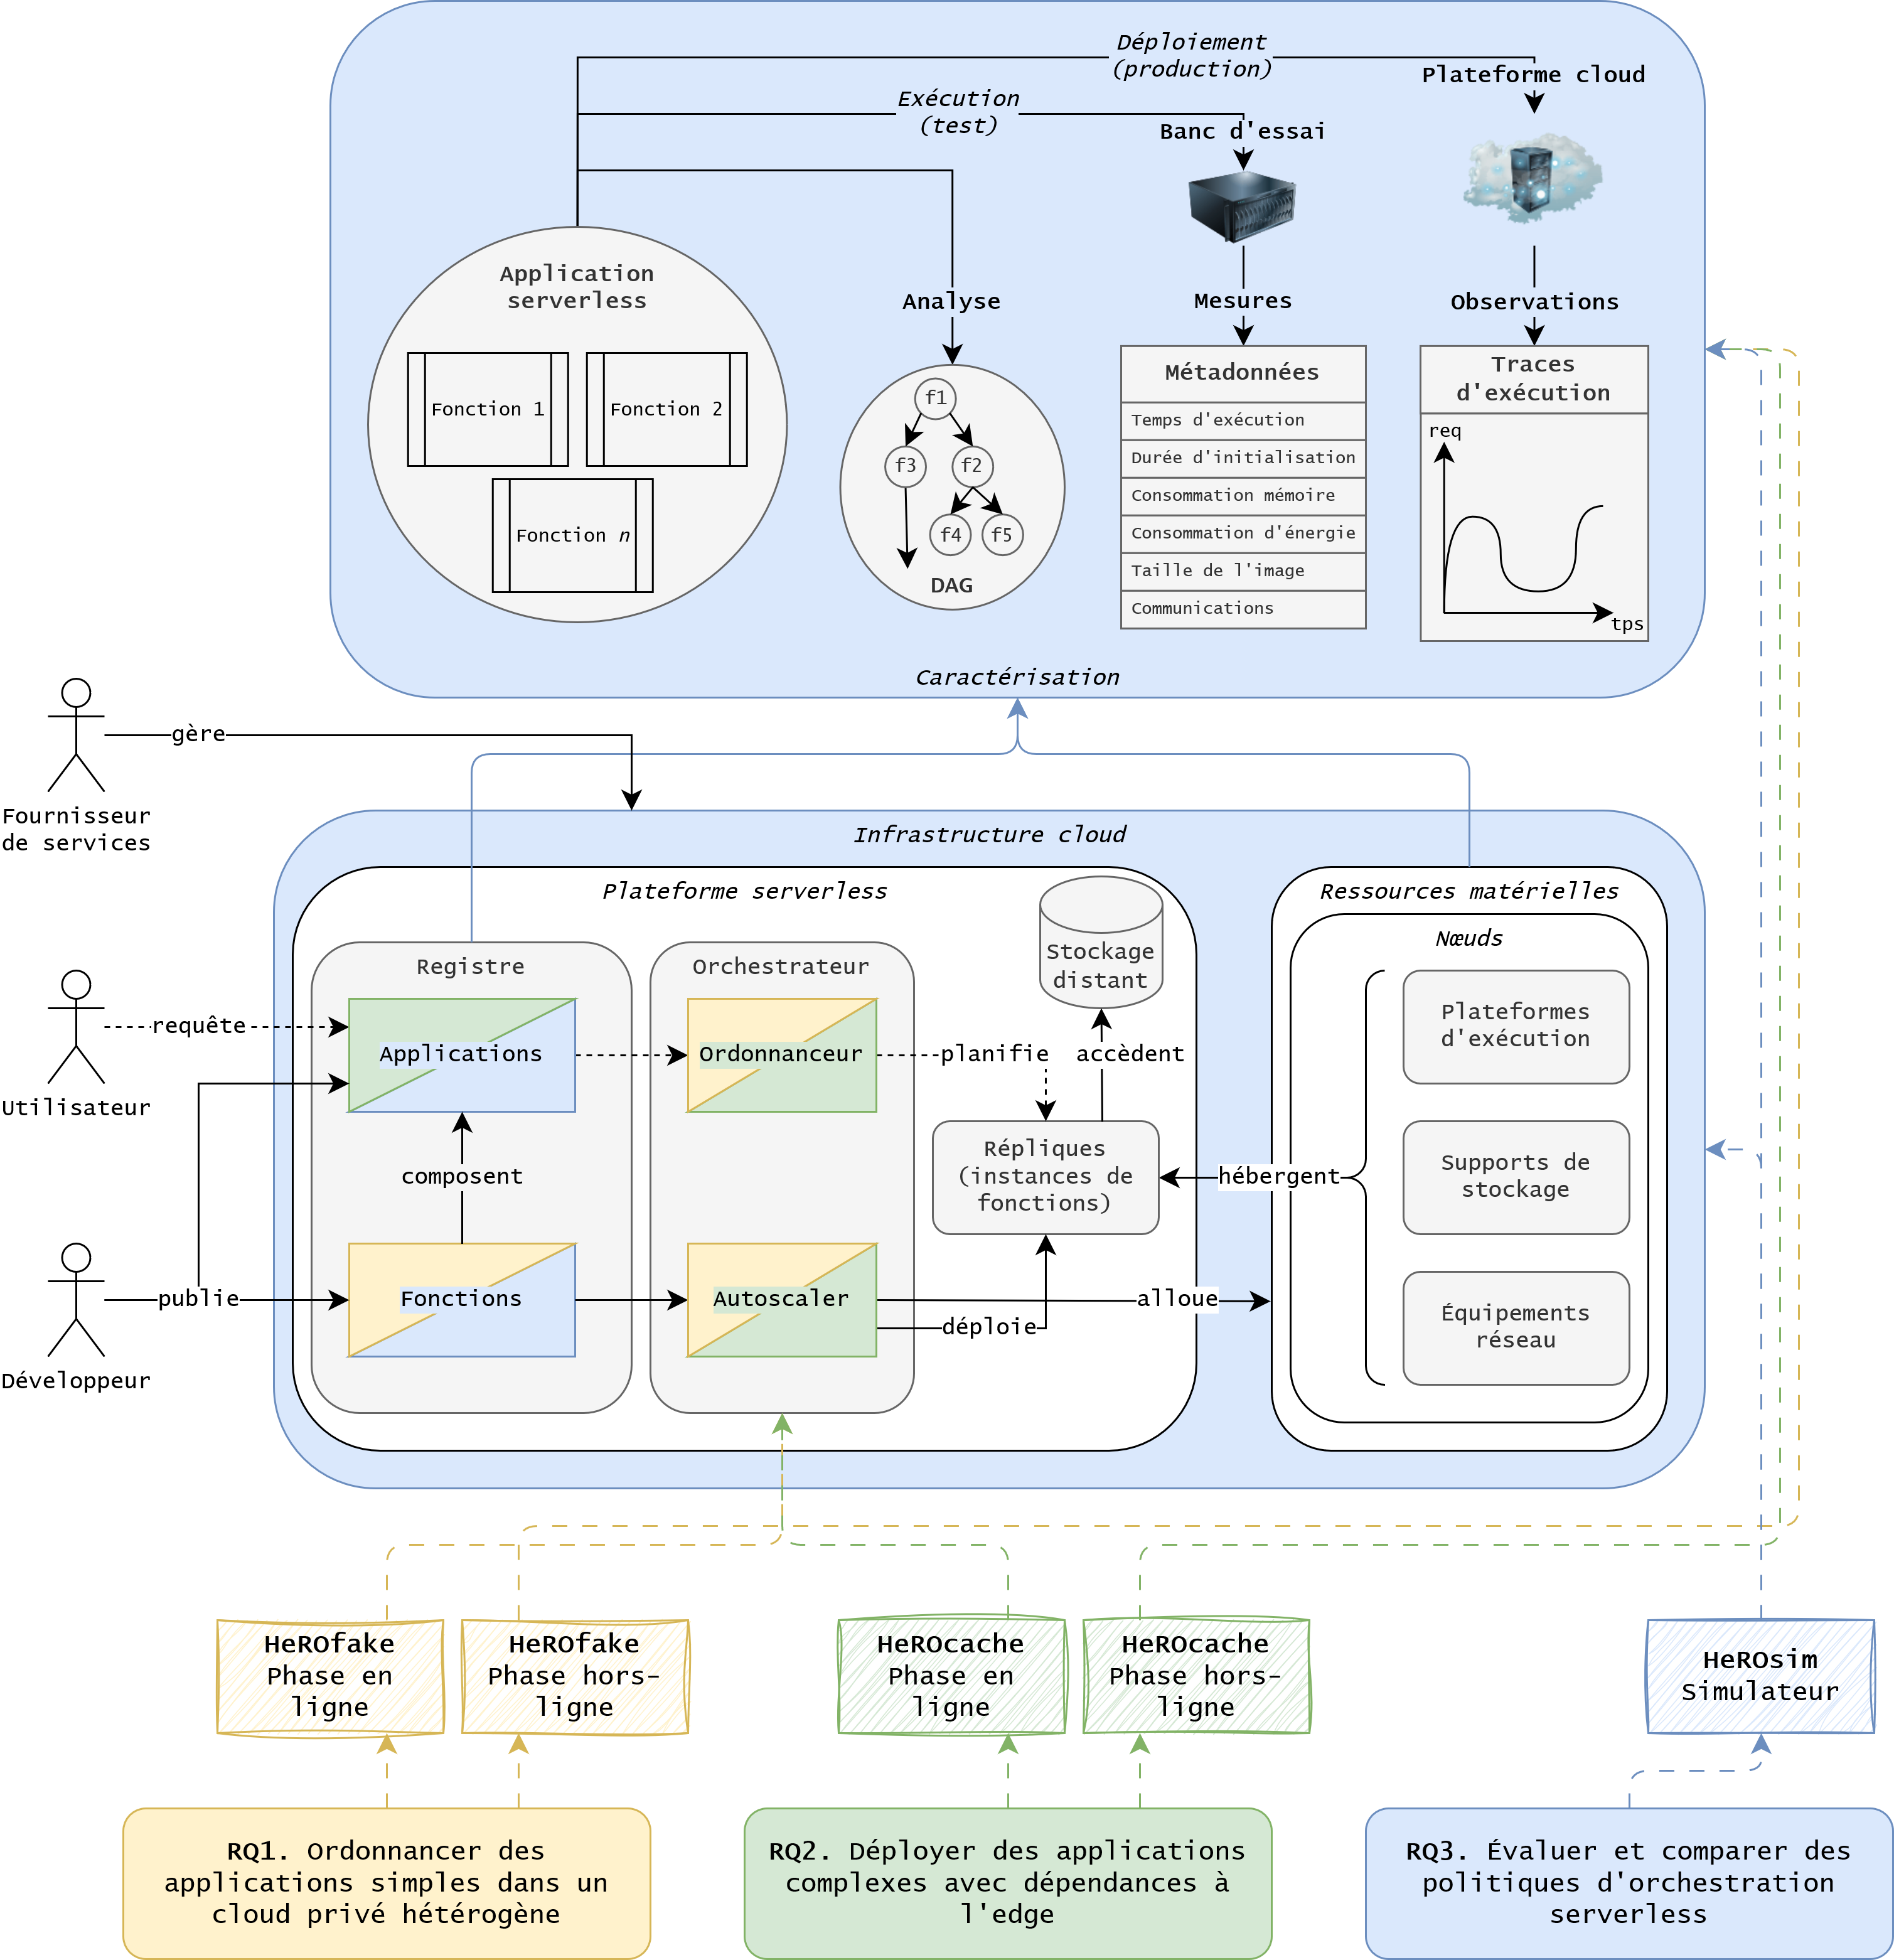
\includegraphics[width=\textwidth]{1_Introduction/figures/architecture.png}
	\caption{Vue à haut niveau de l'architecture considérée, en lien avec nos questions de recherche et nos contributions.}
	\label{figure:intro-architecture}
\end{figure}

Les travaux menés au cours de cette thèse s'inscrivent dans le cadre du modèle de service serverless pour le cloud. Nous avons considéré un environnement dans lequel un fournisseur de services dispose de ressources matérielles que des développeurs peuvent exploiter pour déployer leurs applications à destination d'une variété d'utilisateurs. La figure~\ref{figure:intro-architecture} montre une vue générale de l'architecture du système considéré dans les travaux de cette thèse, ses liens avec nos questions de recherche, ainsi qu'un aperçu du positionnement des contributions au sein de cette architecture.

Les applications, les fonctions et les ressources matérielles sont considérées comme des données d'entrée dans nos contributions. Les applications sont définies par les développeurs ; elles comportent une à plusieurs fonctions, qui peuvent présenter des relations de dépendances (temporelles ou de données) que l'on exprime comme un graphe acyclique (\gls{DAG}, pour \textit{Directed Acyclic Graph}). Les fonctions sont publiées par les développeurs, en vue d'être déployées par la plateforme serverless lors d'une requête utilisateur. Les ressources matérielles constituent l'ensemble des ressources de calcul (processeurs, mémoire, stockage, réseau) disponibles dans l'infrastructure du fournisseur de services. Elles sont réparties au sein de plusieurs nœuds (des serveurs physiques dans le centre de données du fournisseur).

La plateforme serverless comporte une brique logicielle centrale appelée orchestrateur. L'orchestrateur est composé de deux éléments principaux : un \textit{autoscaler}, chargé de l'allocation des ressources matérielles nécessaires au déploiement des fonctions ; ainsi qu'un \textit{ordonnanceur}, responsable de la planification des requêtes utilisateur dans les files d'attente des répliques de fonctions. Les répliques sont des environnements d'exécution pour les instances des fonctions déployées par la plateforme serverless. Les requêtes utilisateur y sont placées en file d'attente avant traitement.

\clearpage

\begin{center}
    \rule{4cm}{0.4pt}
\end{center}

\textbf{Problème 1} -- L'allocation de ressources au sein d'une plateforme serverless se fait sur un mode réactif, c'est-à-dire en réponse à une variation du trafic. Lorsque de nouvelles instances des fonctions doivent être déployées, cela provoque une latence additionnelle qui peut dégrader la qualité de service pour les utilisateurs. Le problème est particulièrement saillant dans l'environnement hautement hétérogène qu'est celui du cloud : les ressources matérielles ont différents niveaux de performances et de coût ; les applications interactives (c'est-à-dire dirigées par les évènements, par opposition à une application par lots) présentent des motifs d'usage difficilement prédictibles ; et les utilisateurs ont des besoins irréguliers et variés en qualité de service.

\boitemagique{Question 1 (\textbf{QR1})}{
    Comment dimensionner les allocations dynamiques de ressources hétérogènes pour une application simple, constituée de fonctions de courte durée, et comment ordonnancer efficacement les requêtes utilisateur, lorsque ces derniers ont des besoins variés en matière de qualité de service ?
}

\begin{center}
    \rule{4cm}{0.4pt}
\end{center}

\textbf{Problème 2} -- Ordonnancer des applications complexes, constituées d'un ensemble de fonctions qui présentent des relations de dépendances et communiquent entre elles des résultats intermédiaires, soulève un problème lié au stockage dans le modèle serverless. En effet, les solutions commerciales s'appuient sur un \textit{stockage distant}, partagé entre les utilisateurs et accédé par le réseau. Ce stockage présente des performances limitées et parfois imprévisibles, notamment du point de vue de la latence, ce qui peut provoquer des délais à chaque étage de l'application. Ces délais s'accumulent alors et provoquent un effet boule de neige, dégradant drastiquement la qualité de service. Par opposition, une possibilité existe d'exploiter le \textit{stockage local} aux nœuds de calcul, c'est-à-dire les supports de stockage physiquement installés sur les serveurs. Mais cela induit un risque de contention sur les ressources, qui peuvent être limitées en capacité et en performances dans le cadre de l'informatique en périphérie (ou \textit{edge}).

\boitemagique{Question 2 (\textbf{QR2})}{
    Comment déployer des applications complexes, composées de chaînes de fonctions de courte durée, et comment tirer parti de l'hétérogénéité des nœuds disponibles à l'edge, pour respecter la qualité de service requise par les utilisateurs tout en contenant la consommation d'énergie de l'infrastructure ?
}

\begin{center}
    \rule{4cm}{0.4pt}
\end{center}

\textbf{Problème 3} -- Évaluer des politiques d'orchestration pour un environnement cloud peut se faire de deux manières différentes : par expérimentation, c'est-à-dire avec du matériel et des utilisateurs réels, ou en simulation. La méthode empirique se heurte à des contraintes de coût d'une part, car il faut réserver une partie de l'infrastructure pour mener les campagnes de mesure. D'autre part, il est complexe d'explorer des scénarios hypothétiques en production, c'est-à-dire de se laisser la liberté de changer un certain nombre de paramètres en entrée pour évaluer leur impact (fréquence des requêtes, caractéristiques du matériel, etc.). Une seconde méthode consiste à modéliser l'environnement cible en s'appuyant sur des simulateurs à l'état de l'art pour le cloud qui, quant à eux, présentent des limites qui rendent délicate la représentation fidèle d'un environnement serverless permettant de comparer les performances de différentes stratégies de gestion des ressources.

\boitemagique{Question 3 (\textbf{QR3})}{
    Du point de vue d'un fournisseur de services pour le cloud, comment évaluer et comparer l'impact sur la qualité de service de différentes politiques d'allocation de ressources et d'ordonnancement de tâches dans le modèle serverless ?
}

\section{Contributions}

Cette section présente les trois contributions principales de la thèse, en indiquant comment elles s'articulent autour des trois questions de recherche précédemment énoncées.

\subsection{Caractérisation et orchestration d'applications simples pour la détection de deepfake}

La \textbf{QR1} (\textit{dimensionnement et ordonnancement pour des applications simples sur ressources hétérogènes}) a émergé d'une réflexion autour du déploiement d'une application sensible à la latence sur des ressources non-réservées au sein de l'IRT b{\textless\textgreater}com. Notre cas d'étude concerne une application de détection de deepfake -- des images ou des vidéos générées numériquement dans un but malicieux, avec l'objectif de tromper leur destinataire en représentant des situations ou des discours qui n'ont pas existé dans la réalité~\cite{westerlundEmergenceDeepfakeTechnology2019}. Cette application est réveillée par l'envoi, par un utilisateur, d'une image à classifier. Elle s'appuie sur des algorithmes d'apprentissage automatique pour déterminer si l'image est en effet synthétique ou bien réelle.

\sloppy Pour répondre à la \textbf{QR1}, nous avons proposé HeROfake (pour \textit{\textbf{He}terogeneous \textbf{R}esources \textbf{O}rchestration for deep\textbf{fake} detection}, voir chapitre~\ref{chapter:herofake}), une plateforme d'orchestration serverless qui vise à réaliser de manière intelligente l'allocation des ressources et l'ordonnancement des requêtes, dans le but d'optimiser l'orchestration pour la qualité de service tout en minimisant la consommation d'énergie du système. Nous avons mené une campagne de mesures afin de caractériser l'exécution d'un ensemble de fonctions d'inférence, utilisées par l'application et basées sur des réseaux de neurones, sur un ensemble de ressources matérielles hétérogènes (\gls{CPU}, \gls{GPU}, \gls{FPGA}). Cette phase de caractérisation permet d'obtenir des métadonnées sur le niveau de performances et de consommation de ressources pour l'application.

Ces métadonnées sont ensuite utilisées par l'orchestrateur lors d'une phase en ligne, afin d'ajuster ses décisions d'allocation et d'ordonnancement tout au long d'un scénario, rejoué en simulation dans un environnement \textit{ad hoc}. Nous avons établi un modèle de coût pour cet orchestrateur, puis conçu une politique d'optimisation multiobjectif visant à minimiser ces fonctions de coût, nourries par les métadonnées issues de la phase de mesures.

Cette contribution a fait l'objet d'une publication dans la conférence \textbf{IEEE/ACM 23rd International Symposium on Cluster, Cloud and Internet Computing} (CCGrid, 2023)~\cite{herofake}.

\subsection{Modèle de coût pour l'orchestration serverless d'applications complexes à l'\textit{edge}}

La \textbf{QR2} (\textit{déploiement d'applications complexes avec dépendances dans le modèle serverless à l'edge}) a émergé pour deux raisons principales. D'une part, comme la suite logique des travaux menés sur la première contribution : si notre précédente contribution permet d'orchestrer des fonctions sans état, nous savons que la plupart des applications ont besoin de stocker des données intermédiaires pendant leur exécution. D'autre part, une étude de la littérature en matière d'orchestration serverless nous a permis de constater que de nombreuses contributions prenaient souvent comme point de départ une situation très favorable, considérant que les images servant à déployer les fonctions sont toujours disponibles sur les nœuds de calcul, et que les communications entre les fonctions sont transparentes du point de vue des performances.

Pour répondre à la \textbf{QR2}, nous avons cherché à établir un modèle de coût pour l'allocation de ressources et l'ordonnancement des tâches qui prenne en compte ces deux mécanismes liés au stockage. Notre cas d'étude pour cette contribution est une application de détection d'intrusions, déployée à l'edge, sur des nœuds hétérogènes aux ressources contraintes et limités en nombre par l'énergie disponible. Nous avons proposé HeROcache (pour \textit{\textbf{He}terogeneous \textbf{R}esources \textbf{O}rchestration with a \textbf{cache} strategy}, voir chapitre~\ref{chapter:herocache}), une stratégie d'orchestration qui cherche à maximiser la consolidation des fonctions d'une même application sur les mêmes nœuds, afin de minimiser la consommation d'énergie de l'infrastructure. Grâce à un mécanisme de mise en cache des données sur le stockage local, cette stratégie permet de réduire les délais de communication des applications et limite les violations de qualité de service.

Cette contribution a fait l'objet d'une publication dans la conférence \textbf{IEEE/ACM 24rd International Symposium on Cluster, Cloud and Internet Computing} (CCGrid, 2024)~\cite{herocache}.

\subsection{Simulation à événements discrets pour l'évaluation de politiques d'orchestration}

La \textbf{QR3} (\textit{évaluer et comparer différentes politiques d'orchestration serverless}) a été transversale tout au long des travaux de thèse. Concevoir des stratégies d'allocation et d'ordonnancement pour le cloud demande d'avoir à notre disposition un environnement dans lequel les évaluer.

Pour répondre à la \textbf{QR3}, nous avons proposé et développé HeROsim (pour \textit{\textbf{He}terogeneous \textbf{R}esources \textbf{O}rchestration \textbf{sim}ulator}, voir chapitre~\ref{chapter:herosim}), un simulateur \textit{open source} à événements discrets pour le cloud serverless, qui présente les caractéristiques nécessaires à la modélisation fine d'un environnement serverless et l'évaluation de politiques d'orchestration. La simulation progresse à une granularité au niveau d'une requête utilisateur, et permet de modéliser des applications complexes (dépendances entre les fonctions) et des environnements hétérogènes (nœuds à différents niveaux de performances, requêtes à différents niveaux de qualité de service). HeROsim permet de rejouer des scénarios (sur la base de traces d'exécution) et de comparer les résultats de différentes politiques au regard de métriques de qualité de service et de consommation d'énergie.

Cette contribution a fait l'objet d'une publication dans le journal \textbf{IEEE Internet Computing} (\textit{Special Issue on Serverless Computing})~\cite{herosim} en fin d'année 2024.

\section{Cadre des travaux}

Cette thèse s'est conduite en partenariat entre le Lab-STICC et l'Institut de Recherche Technologique (IRT) b{\textless\textgreater}bcom~\footnote{\href{https://b-com.com/}{https://b-com.com/}}, créé en 2012. b{\textless\textgreater}bcom est l'un des huit IRT français. Son ambition est de fournir des solutions numériques au service des entreprises et de leur compétitivité. Il est particulièrement actif dans les domaines des télécommunications, de l'audiovisuel et de l'immersion.

Les travaux de cette thèse se sont inscrits dans deux projets au sein de l'IRT. Dans le cadre du projet SUPRA d'abord, qui entend livrer un système de cloud souverain pour les applications télécom, e-santé et intelligence artificielle sur des infrastructures en propre. Les travaux de thèse se sont poursuivis tout au long du projet RPC (\textit{Réseaux Privés Cellulaires}) ensuite, un axe transversal à b{\textless\textgreater}com qui mobilise une grande partie des équipes, dans le but de concevoir un système souverain de radio logicielle (RAN, pour \textit{Radio Access Network}), déployé dans un environnement virtualisé et distribué entre cloud et edge.

\clearpage

\section{Organisation de la thèse}

Ce manuscrit est composé de sept chapitres (dont cette introduction), organisés comme suit :

\begin{center}
    \rule{4cm}{0.4pt}
\end{center}

\textbf{Partie~\ref{part:one} : Contexte et état de l'art}

Le chapitre~\ref{chapter:context} décrit l'environnement général des travaux de la thèse, et donne en particulier les caractéristiques du cloud et du modèle serverless. Le chapitre~\ref{chapter:sota} présente des contributions de l'état de l'art dans le domaine de l'orchestration dynamique pour le cloud.

\begin{center}
    \rule{4cm}{0.4pt}
\end{center}

\textbf{Partie~\ref{part:two} : Contributions}

Cette partie présente les trois contributions de la thèse. Le chapitre~\ref{chapter:herofake} décrit notre solution d'allocation et d'ordonnancement dynamiques sous contrainte de qualité de service pour des fonctions simples, ainsi que notre méthodologie de caractérisation des plateformes et des tâches. Le chapitre~\ref{chapter:herocache} présente notre orchestrateur s'appuyant sur un modèle de coût intégrant les problématiques de stockage pour le serverless. Le chapitre~\ref{chapter:herosim} détaille l'environnement de simulation développé dans le cadre de la thèse pour évaluer des politiques d'orchestration serverless pour le cloud.

\begin{center}
    \rule{4cm}{0.4pt}
\end{center}

\textbf{Partie~\ref{part:three} : Conclusion et perspectives}

Enfin, le chapitre~\ref{chapter:conclusion} résume les contributions de la thèse et présente les limites identifiées dans les solutions proposées, pour ouvrir la discussion sur des perspectives de futurs travaux.


\part{Contexte et état de l'art}
\label{part:one}

\clearemptydoublepage
\mainmatter
\clearemptydoublepage
\chapter{Contexte -- Cloud, ordonnancement et élasticité}
\label{chapter:context}

Dans ce deuxième chapitre, nous donnons une définition formelle du cloud, au travers des propriétés spécifiques à ces environnements de calcul et de stockage partagés. Nous présentons également quelques techniques et technologies socles dans les centres de données. Enfin, nous commentons les caractéristiques des applications déployées dans le cloud, et terminons par introduire le modèle serverless pour le cloud, qui constitue l'environnement au cœur des problématiques traitées au cours de cette thèse.

\section{\textit{Cloud computing} : une définition}

Les premières réflexions autour de l'émergence d'un système informatique à temps partagé remontent au début des années 1960~\cite{greenberger1962management}. L'idée, nouvelle, est alors de permettre le partage des ressources matérielles d'une part entre différentes tâches, et d'autre part entre différents utilisateurs~\cite{meyerVirtualMachineTimesharing1970}. L'objectif est de maximiser l'utilisation des ressources en permettant à plusieurs utilisateurs d'exploiter la même machine simultanément, limitant ainsi le gaspillage de temps de calcul~\cite{corbato1962experimental}.
%Le premier objectif est bien sûr de maximiser l'utilisation des ressources, mais les auteurs considèrent également ce problème sous un angle différent : le taux -- ou la vitesse -- d'interaction entre utilisateurs et machines. À cette époque, le constat suivant est déjà établi : la vitesse de calcul d'un ordinateur surpasse la vitesse à laquelle son utilisateur peut le programmer. Permettre à plusieurs personnes d'utiliser la même machine simultanément permettrait de limiter le gaspillage de temps de calcul~\cite{corbato1962experimental}.

Le cloud est vu comme la suite logique au succès de ces systèmes à temps partagé~\cite{hayesCloudComputing2008}. Salesforce fait partie des premières sociétés à avoir fait le pari du cloud en 1999~\cite{weissmanDesignForceCom2009} en proposant à ses clients une suite logicielle d'informatique de gestion accessible en ligne. En 2006, Amazon Web Services (\gls{AWS}) propose EC2~\footnote{\href{https://aws.amazon.com/fr/ec2/}{https://aws.amazon.com/fr/ec2/}} (pour \textit{Elastic Compute Cloud}), la première offre d'infrastructure en tant que service. La même année, Google lance Google Docs~\footnote{\href{https://www.google.fr/intl/fr/docs/about/}{https://www.google.fr/intl/fr/docs/about/}}, une suite bureautique accessible en ligne et destinée aux utilisateurs finaux. En 2010, la NASA annonce la publication sous licence libre d'OpenStack~\footnote{\href{https://www.openstack.org/}{https://www.openstack.org/}}, une plateforme logicielle permettant de gérer une infrastructure cloud, ouvrant la possibilité à de nouveaux acteurs de rentrer sur le marché du cloud sans avoir à développer une pile logicielle complète.

Le cloud apparaît donc comme un environnement hautement hétérogène pour lequel il convient d'avoir des éléments de définition communément admis.

\subsection{Caractéristiques}

Le \gls{NIST} donne une définition formelle du cloud~\cite{mellNISTDefinitionCloud} en établissant les caractéristiques essentielles d'une telle plateforme :

\begin{itemize}
    \item \textbf{Service à la demande} -- Les clients réservent des ressources matérielles de manière autonome, par exemple au travers d'une interface web, sans interagir avec un opérateur. En retour, ils n'ont généralement pas de contrôle fin sur la localité précise des ressources réservées ;
    \item \textbf{Accessible par le réseau} -- Ces ressources sont immédiatement mises à disposition des clients et accessibles par Internet ;
    \item \textbf{Partage des ressources} -- La puissance de calcul, les capacités de stockage et la bande passante sont partagées entre les clients du fournisseur de services. Des techniques de virtualisation sont mises en œuvre pour isoler les tâches déployées ;
    \item \textbf{Élasticité rapide} -- Les clients peuvent à tout moment décider d'augmenter ou de diminuer la quantité et les caractéristiques des ressources qu'ils réservent, de manière à garantir les performances de leurs applications ou maîtriser leurs coûts ;
    \item \textbf{Service mesuré} -- Les infrastructures cloud sont instrumentées de manière à fournir aux clients une information précise sur leur consommation de ressources, et les coûts monétaires associés.
\end{itemize}

\subsection{Modèles de service}

\begin{figure}[!ht]
    \centering
	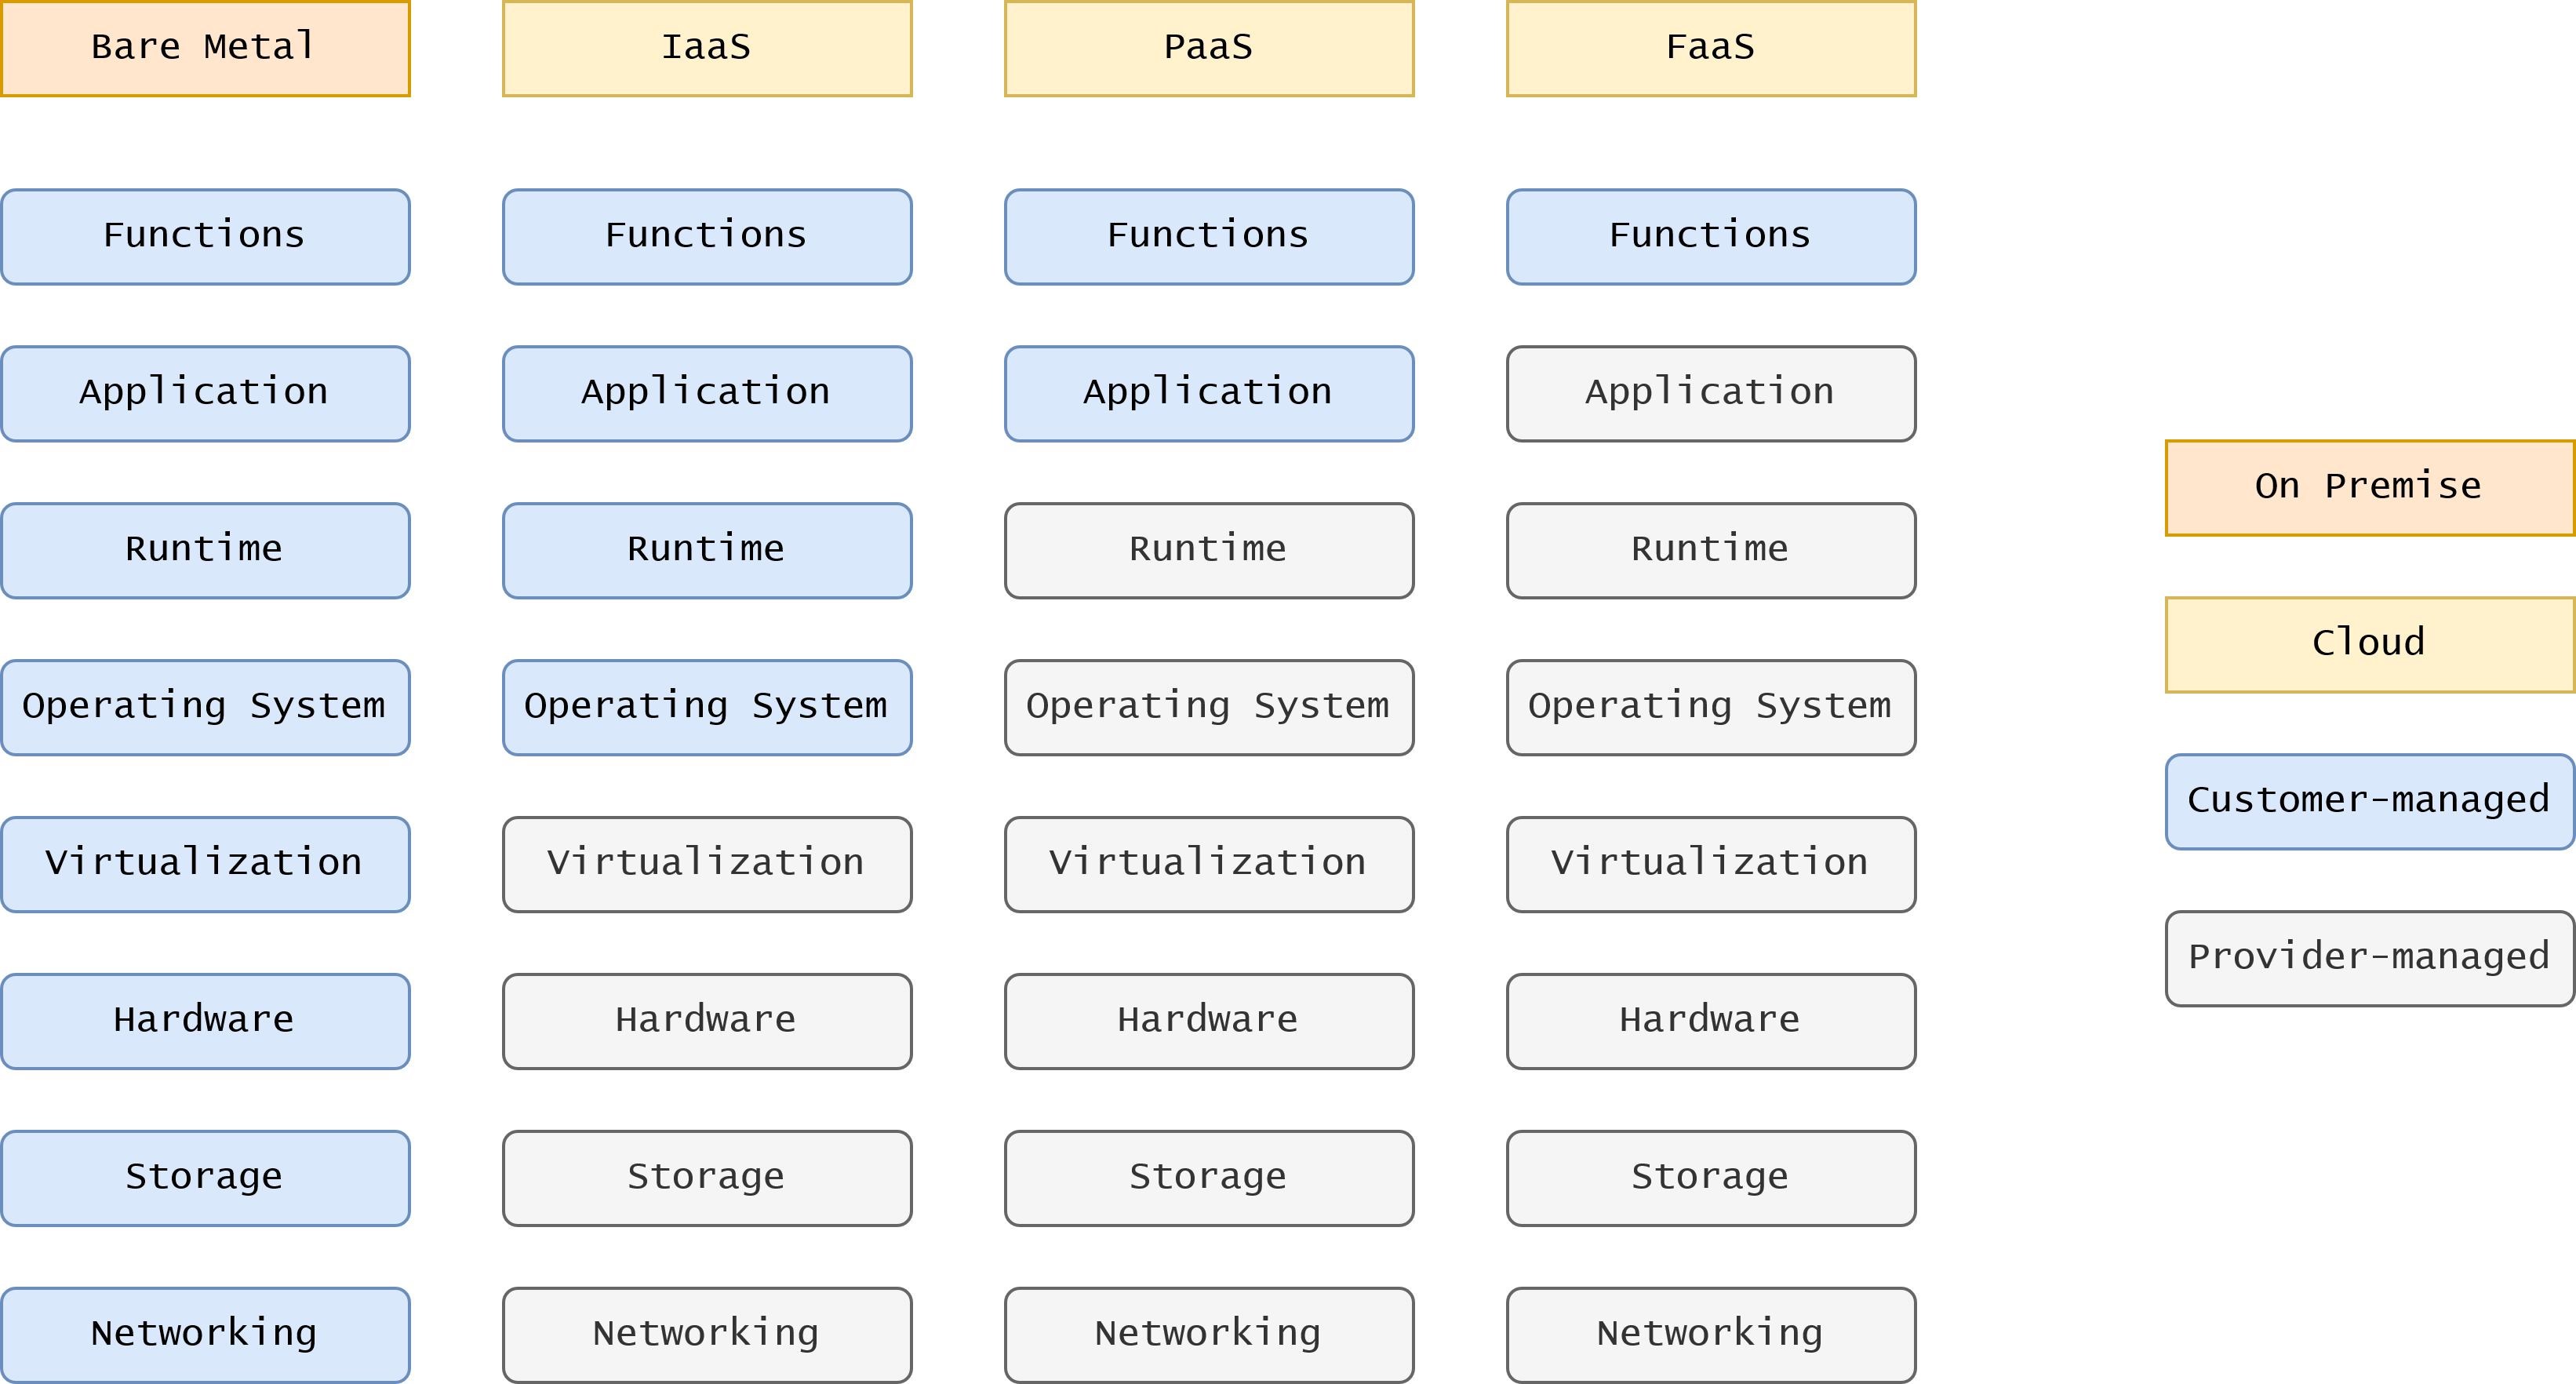
\includegraphics[width=\textwidth]{2_Chapitre2/figures/service-models.png}
	\caption[Comparaison entre différents modèles de service pour le cloud en termes de responsabilités pour le client et le fournisseur de service.]{Comparaison entre différents modèles de service pour le cloud en termes de responsabilités pour le client et le fournisseur de service (inspiré de la documentation Red Hat~{\protect \footnotemark}).}
	\label{figure:context-service-model}
\end{figure}

\footnotetext{\href{https://www.redhat.com/en/topics/cloud-computing/iaas-vs-paas-vs-saas}{https://www.redhat.com/en/topics/cloud-computing/iaas-vs-paas-vs-saas}}

Ces caractéristiques sont déclinées dans trois modèles de service, comme illustré par la figure~\ref{figure:context-service-model}, qui constituent des déclinaisons de l'offre commerciale des fournisseurs de service cloud :

\begin{itemize}
    \item \textbf{Infrastructure as a Service} (\gls{IaaS}) -- Cible les clients qui souhaitent un contrôle à grain fin sur leurs infrastructures. Les clients sont responsables de l'administration des ressources matérielles mises à leur disposition, c'est-à-dire des serveurs, souvent virtuels (voir section~\ref{section:background-virtualization}) ;
    \item \textbf{Platform as a Service} (\gls{PaaS}) -- Cible les clients qui souhaitent déployer leurs applications sans avoir la responsabilité d'administration des serveurs ;
    \item \textbf{Software as a Service} (\gls{SaaS}) -- Cible l'utilisateur final en offrant l'accès à une application entièrement administrée par le fournisseur de services.
\end{itemize}

\subsection{Modèles de déploiement}

Pour organiser les calculs et les données dans le cloud, il existe plusieurs stratégies qui correspondent à différentes contraintes métier pour les utilisateurs :

\begin{itemize}
    \item \textbf{Cloud privé} -- L'infrastructure est dédiée à une organisation qui regroupe plusieurs utilisateurs finaux. Ce modèle de déploiement est privilégié par les clients pour la sécurité et la confidentialité des données ;
    \item \textbf{Cloud public} -- L'infrastructure est partagée entre de nombreux clients hétérogènes, professionnels comme particuliers. Ce modèle de déploiement est souvent moins coûteux pour le client qu'une offre de cloud privé ;
    \item \textbf{Cloud communautaire} -- L'infrastructure est partagée entre différents acteurs ayant souvent des problématiques métier similaires (secteurs bancaire ou hospitalier par exemple) ;
    \item \textbf{Cloud hybride} -- Solution de répartition des tâches entre cloud privé et cloud public, en fonction de leur niveau de criticité.
\end{itemize}

\section{Ordonnancement dans le cloud}

Dans cette section, nous présentons les techniques mises en œuvre par les fournisseurs de services cloud pour partager les ressources matérielles et isoler les charges de travail de leurs différents utilisateurs. Nous introduisons les défis pour la mise à l'échelle de ces ressources lors de variations de charge sur les applications déployées, notamment en matière de qualité de service.

\subsection{Virtualisation dans un cadre multi-tenant}
\label{section:background-virtualization}

Le modèle économique des fournisseurs de services pour le cloud repose sur la mutualisation des ressources matérielles entre de nombreux clients~\cite{hayesCloudComputing2008}. Les plateformes cloud doivent donc prendre en charge un nombre important de traitements, ce qui entraîne une situation de partage massif des ressources matérielles qui nécessite des techniques d'isolation et de virtualisation adéquates~\cite{vaqueroLockingSkySurvey2011}. C'est ce que l'on appelle le cadre multi-tenant~\cite{weissmanDesignForceCom2009}.

Comme les ressources sont mises en commun et que différentes applications les utilisent, cela ouvre des canaux, auxiliaires ou non, vecteurs potentiels d'attaques entre les processus dans l'espace utilisateur~\cite{pedersen2017trash, wu2018side}. Bénéficier du cadre multi-tenant s'accompagne donc de la responsabilité, pour le fournisseur, de garantir la confidentialité et la sécurité des données et des différentes charges de travail des clients~\cite{vaqueroLockingSkySurvey2011}.

Pour respecter ces garanties, les fournisseurs doivent recourir à des mesures de protection pour assurer le cloisonnement entre différents processus appartenant à des applications et/ou des utilisateurs différents. Ce mécanisme consistant à présenter, de manière transparente, un environnement d'exécution distinct avec un espace d'adressage, un système de fichiers et des autorisations propres à chaque processus est appelé isolation~\cite{fehlingCloudComputingPatterns2014}. À cette fin, les fournisseurs peuvent s'appuyer sur des technologies de virtualisation.

La virtualisation est une technique d'isolation qui permet d'exécuter une application dans les limites d'un environnement d'exécution sécurisé, en introduisant une couche d'indirection entre la plateforme hôte et l'application elle-même~\cite{singhviAtollScalableLowLatency2021}.

La virtualisation des ressources de l'hôte peut se faire à l'aide de machines virtuelles (\gls{VM}, pour \textit{Virtual Machine}) ou de conteneurs. Ces environnements d'exécution donnent aux processus sous-jacents l'illusion d'avoir une machine entière à leur disposition. Alors que les VM virtualisent les ressources physiques de l'hôte, en s'appuyant sur l'architecture du processeur pour réaliser l'isolation, les conteneurs exploitent des directives du système d'exploitation hôte pour isoler les charges de travail~\cite{mancoMyVMLighter2017}.

Lorsqu'ils choisissent le modèle d'isolation sur lequel ils souhaitent s'appuyer pour exploiter le partage des ressources, les fournisseurs cloud doivent faire un compromis entre performances et sécurité. Les conteneurs sont fréquemment la cible d'attaques par élévation de privilèges~\cite{zomer2022containers, redhat2019containers}, mais leurs temps de démarrage sont de plusieurs ordres de grandeur inférieurs à ceux des machines virtuelles : le temps d'initialisation des conteneurs se compte en centaines de millisecondes, tandis que les VM démarrent en quelques secondes~\cite{mancoMyVMLighter2017}. La conception de machines virtuelles légères offrant des temps d'initialisation comparables à ceux des conteneurs est un sujet de recherche essentiel~\cite{agacheFirecrackerLightweightVirtualization, Anjali2020BlendingCA}.

\begin{figure}[!ht]
    \centering
	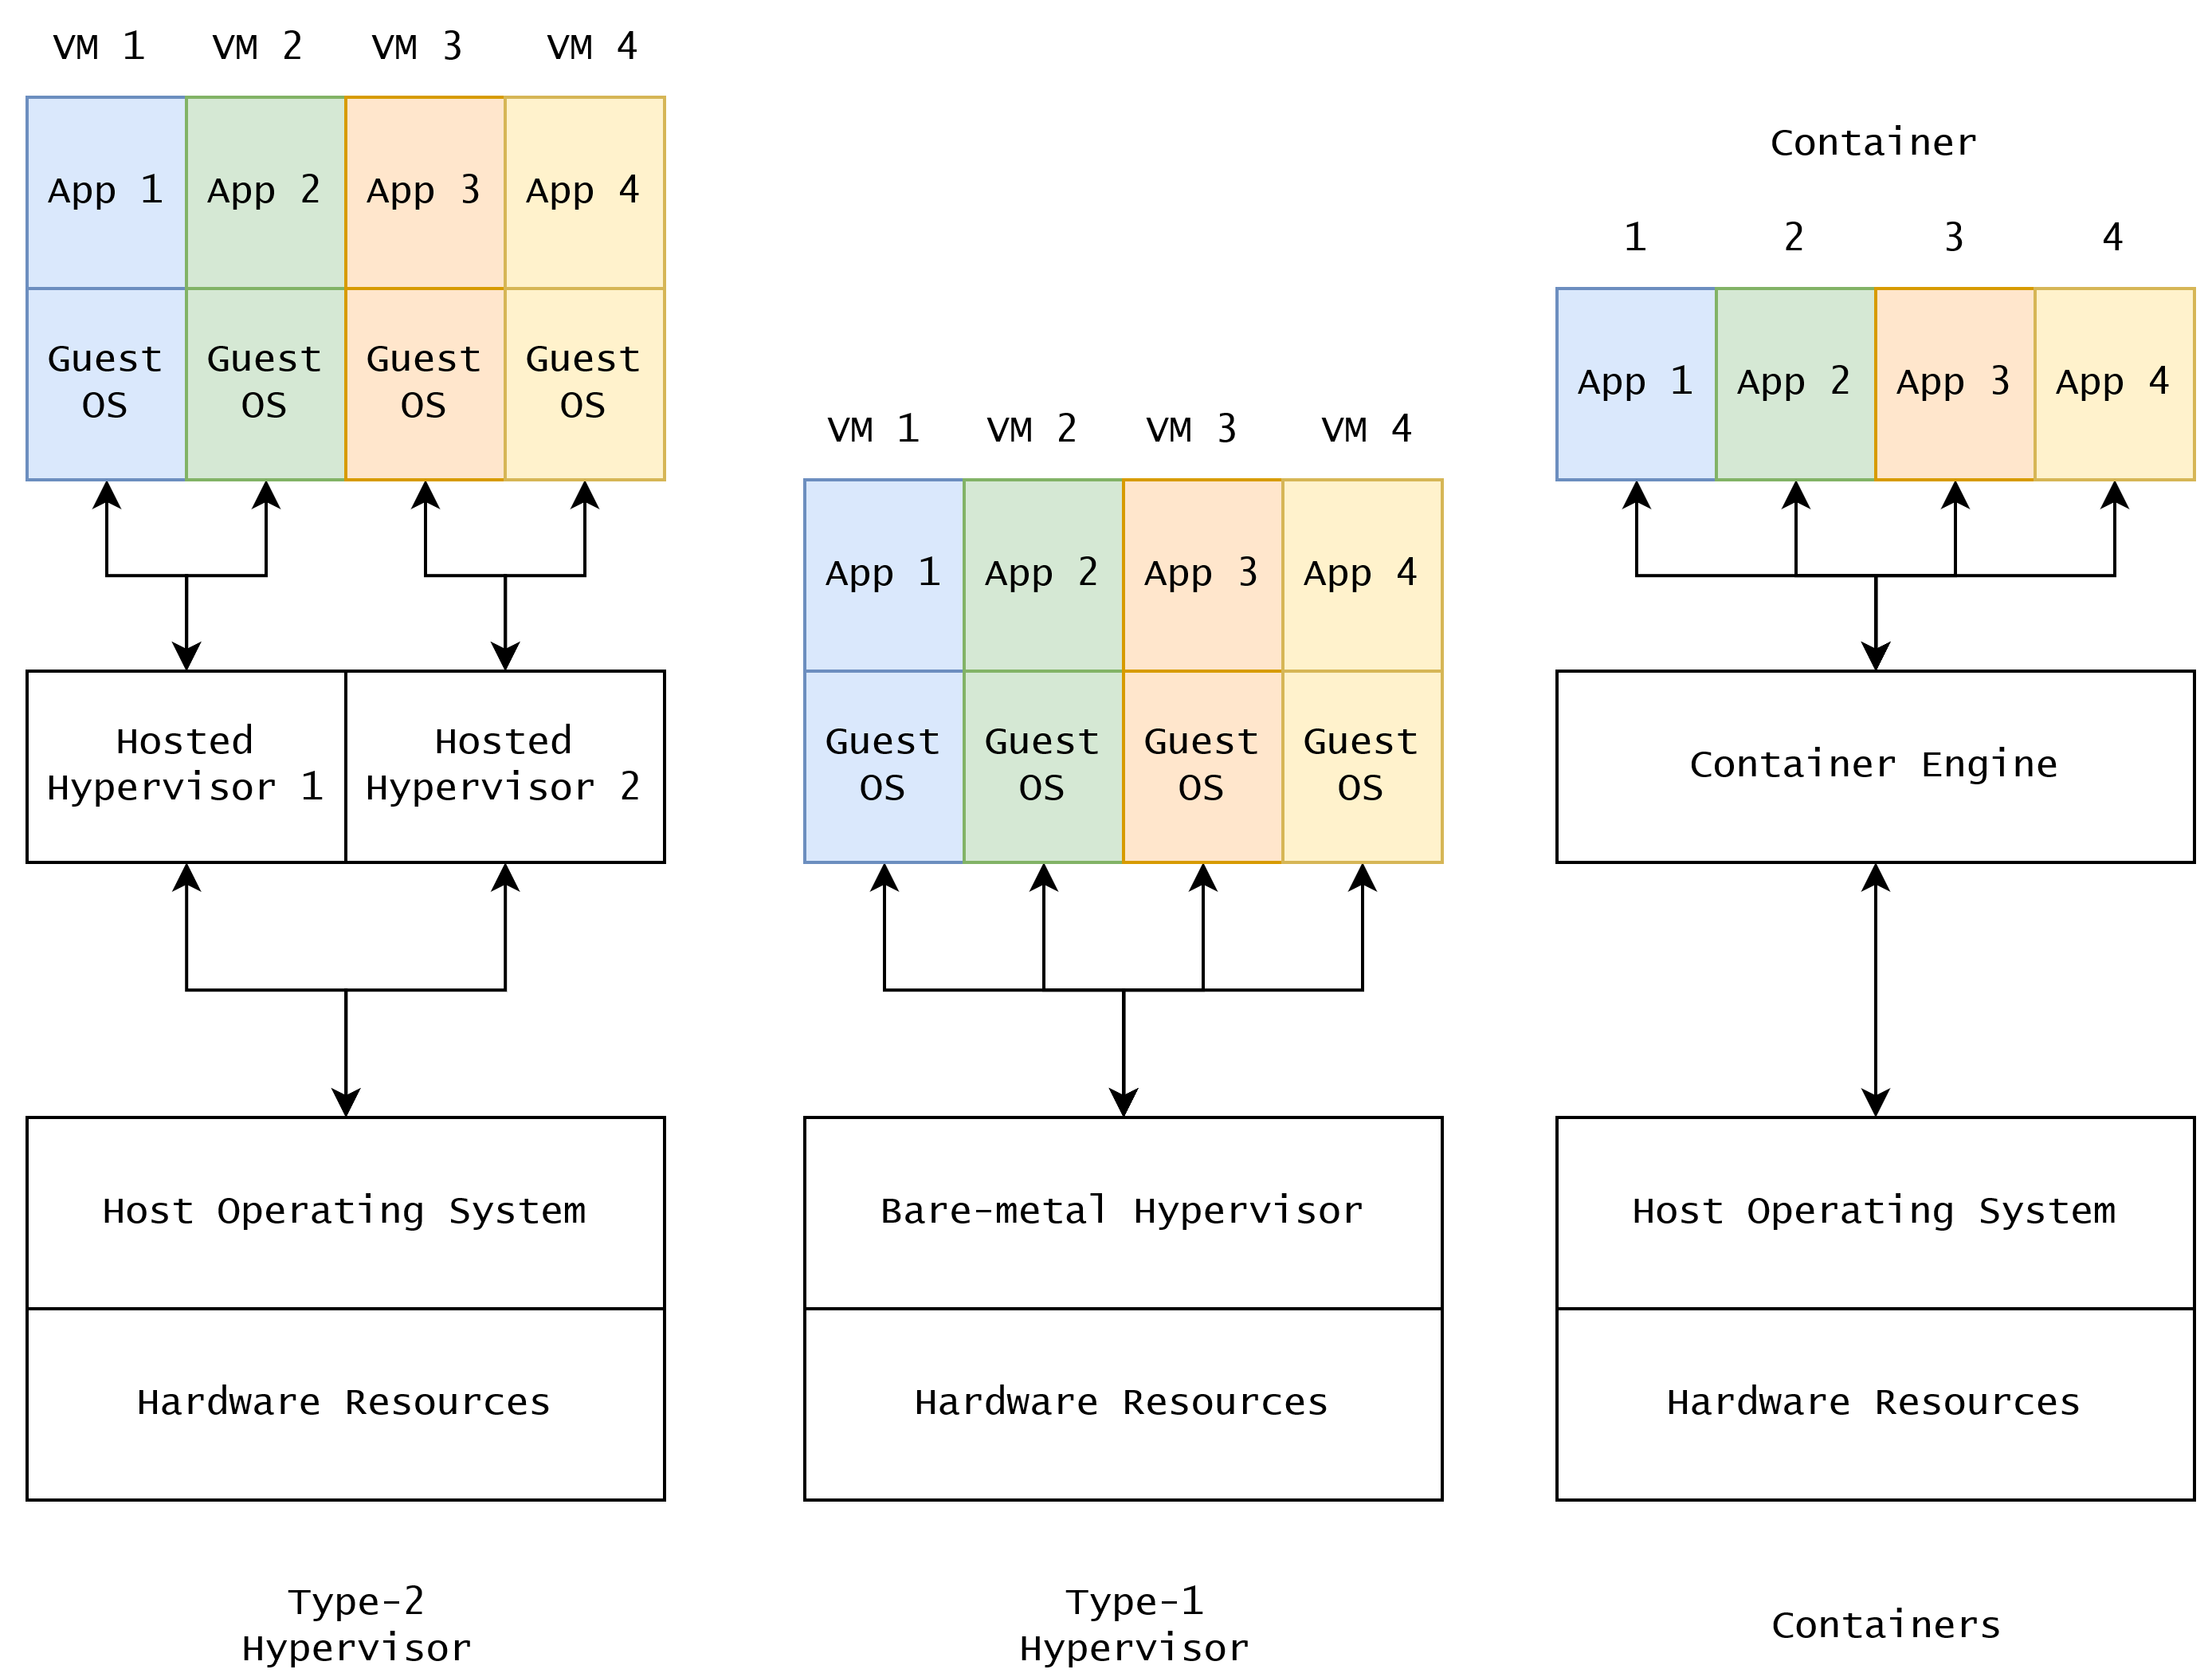
\includegraphics[width=\textwidth]{2_Chapitre2/figures/virtualization.png}
	\caption{Aperçu des différents modèles d'isolation : virtualisation (avec hyperviseurs de types 1 et 2) et conteneurisation.}
	\label{figure:context-virtualization}
\end{figure}

\subsubsection{Machines virtuelles}

La virtualisation assistée par le matériel permet à plusieurs systèmes d'exploitation \textit{invités} complets de fonctionner indépendamment sur des ressources physiques partagées, quelle que soit la nature du système d'exploitation \textit{hôte}~\cite{kivityKvmLinuxVirtual}.

Du point de vue d'une application déployée dans une VM, l'environnement d'exécution isolé est perçu comme une plateforme complète, alors qu'il s'agit en réalité d'un sous-ensemble des ressources de la plateforme hôte, déterminé par l'hyperviseur (ou \gls{VMM}, pour \textit{Virtual Machine Manager}), un logiciel de bas niveau qui peut faire office de système d'exploitation, ou s'exécuter en tant que processus du système d'exploitation hôte.

L'hyperviseur a la responsabilité de gérer le cycle de vie des machines virtuelles : la création, l'exécution, la destruction et parfois la migration des machines virtuelles sont gérées par l'hyperviseur.

Les hyperviseurs existent sous deux formes différentes, comme illustré dans la figure~\ref{figure:context-virtualization} :

\begin{itemize}
    \item Les hyperviseurs de type 1 (\textit{bare-metal}) s'exécutent directement sur le matériel de la machine hôte. Étant donné qu'ils ne dépendent pas d'un système d'exploitation (\gls{OS}, pour \textit{Operating System}) sous-jacent, ils sont considérés comme plus sûrs et plus efficaces que leurs homologues hébergés. Parmi les exemples courants d'hyperviseurs de type 1, on trouve VMware ESXi~\footnote{\href{https://www.vmware.com/products/cloud-infrastructure/esxi-and-esx}{https://www.vmware.com/products/cloud-infrastructure/esxi-and-esx}}, Linux KVM~\footnote{\href{http://www.linux-kvm.org/}{http://www.linux-kvm.org/}}, Xen~\footnote{\href{https://xenproject.org/}{https://xenproject.org}} et Microsoft Hyper-V~\footnote{\href{https://learn.microsoft.com/en-us/virtualization/hyper-v-on-windows/about/}{https://learn.microsoft.com/en-us/virtualization/hyper-v-on-windows/about/}} ;
    \item Les hyperviseurs de type 2 (hébergés) s'exécutent au-dessus d'un système d'exploitation. Ces hyperviseurs sont des produits grand public qui offrent aux utilisateurs finaux un moyen pratique d'exécuter des systèmes ou des programmes qui ne seraient pas nativement pris en charge par leur matériel ou leur système d'exploitation. Parmi les hyperviseurs de type 2, on peut citer QEMU~\footnote{\href{https://www.qemu.org/}{https://www.qemu.org}} et Oracle VirtualBox~\footnote{\href{https://www.virtualbox.org/}{https://www.virtualbox.org/}}.
\end{itemize}

\subsubsection{Conteneurs}

La conteneurisation est une technique de virtualisation au niveau du système d'exploitation. Le noyau du système d'exploitation hôte est responsable de l'allocation des ressources. Les conteneurs virtualisent le système d'exploitation : ils donnent au processus conteneurisé l'impression d'avoir toute la machine à leur disposition, tout en étant en réalité contraint et limité en ce qui concerne l'utilisation des ressources par le noyau hôte~\cite{bentalebContainerizationTechnologiesTaxonomies2022}.

Les conteneurs constituent un mécanisme d'isolation léger qui repose sur les capacités d'isolation du noyau du système hôte, comme le montre la figure~\ref{figure:context-virtualization}. En l'occurrence, sous Linux :

\begin{itemize}
    \item \texttt{chroot} : modifie le répertoire racine apparent pour une arborescence de processus donnée. Il permet à un conteneur d'opérer sur un répertoire virtuel \texttt{/} qui pourrait être situé n'importe où sur le système de fichiers de l'hôte ;
    \item \texttt{cgroups} : permettent de créer des groupes hiérarchiques de processus et allouer, limiter et surveiller les ressources matérielles pour ces groupes : E/S vers et depuis les périphériques de bloc, accès à l'unité centrale, à la mémoire et aux interfaces réseau ;
    \item \texttt{namespaces} : une couche d'abstraction autour des ressources du système d'exploitation, telles que le réseau ou les communications entre processus (IPC). Les processus au sein d'un espace de noms ont leurs propres instances isolées de ces ressources système.
\end{itemize}

L'ambition derrière les conteneurs est de contenir l'exécution d'une application dans un processus isolé du reste du système, de sorte à ce qu'il ignore les autres processus exécutés par le système hôte. Le cycle de vie des conteneurs est géré par un moteur de conteneurs. Le conteneur est amorcé à partir d'une image qui contient toutes les dépendances nécessaires à la construction et/ou à l'exécution de l'application.

Dans l'écosystème des conteneurs, Docker~\footnote{\href{https://www.docker.com/}{https://www.docker.com/}} en particulier a connu une forte progression depuis sa création en 2013. Docker a joué un rôle déterminant dans la spécification des normes industrielles pour les formats de conteneurs par le biais de l'\textit{Open Container Initiative}~\footnote{\href{https://opencontainers.org/}{https://opencontainers.org/}} (OCI), qui définit les spécifications des images de conteneurs - des lignes directrices sur la manière de créer une image OCI avec son manifeste, ses couches de système de fichiers et sa configuration - et les spécifications d'exécution concernant la manière d'exécuter les paquets d'applications au fur et à mesure qu'ils sont décompressés sur le système d'exploitation hôte.

\subsection{Dimensionnement : équilibrage de charge et passage à l'échelle}

Dans le cloud, les applications sont souvent déployées sur plusieurs zones géographiques (différents centres de données), et sur plusieurs nœuds (serveurs) au sein de l'infrastructure~\cite{hayesCloudComputing2008}. Chaque déploiement de l'application est appelé "instance".

Une brique logicielle essentielle dans une plateforme cloud est le \textit{load balancer}. Son rôle est de distribuer les requêtes entrantes (\textit{i.e.} la charge) pour une application entre les différentes instances déployées~\cite{jafarnejadghomiLoadbalancingAlgorithmsCloud2017}. Ce processus doit être transparent du point de vue des utilisateurs de l'application, qui ne savent pas quelle instance répond à leurs requêtes.

L'équilibrage de charge s'appuie sur des politiques (ou stratégies) de gestion des ressources qui peuvent viser différents objectifs. Un fournisseur de services peut chercher à répartir la charge autant que possible de manière à minimiser la latence des requêtes ; à l'inverse, il peut chercher à consolider les tâches sur un nombre réduit de nœuds, afin de réduire la consommation d'énergie de la plateforme~\cite{leeEnergyEfficientUtilization2012}.

Lorsque la charge sur une application augmente, une mise à l'échelle (ou \textit{scaling}) des ressources matérielles qui lui sont allouées peut alors être effectuée selon deux axes :

\begin{itemize}
    \item \textbf{Verticalement}~\cite{boyd-wickizerAnalysisLinuxScalability, linderOracleParallelRDBMS1993, xian-hesunScalabilityParallelAlgorithmmachine1994} : en attachant plus de ressources matérielles aux serveurs qui supportent l'application (par exemple, augmenter le nombre de CPU ou la quantité de mémoire alloués à une VM). Il peut s'agir de migrer une instance de l'application vers un nouveau serveur plus performant, ce qui a un impact sur la disponibilité de l'application. Le mécanisme d'équilibrage de charge permet de router temporairement les requêtes entrantes vers une instance fonctionnelle de l'application en attendant l'initialisation de la nouvelle instance ;
    \item \textbf{Horizontalement}~\cite{al-faresHederaDynamicFlow, lakshmanCassandraDecentralizedStructured2010, weilCephScalableHighPerformance} : en augmentant le nombre de serveurs alloués à l'application. Le mécanisme d'équilibrage de charge permet d'acheminer les requêtes et les réponses entre les utilisateurs et les multiples instances de l'application.
\end{itemize}

L'opération contraire peut être symétrique, ou non, lorsque le nombre ou la complexité des traitements diminue.

\subsection{Qualité de service et métriques de performances}

Les fournisseurs de services cloud sont souvent tenus à des engagements (\gls{SLA}, pour \textit{Service Level Agreement}) en matière de qualité de service (\gls{QoS}, pour \textit{Quality of Service}). Ils s'engagent auprès de leurs clients sur un certain nombre de critères (\gls{SLO}, pour \textit{Service Level Objective}) mesurés par des métriques telles que la latence, le débit, la disponibilité, etc. En cas de violation de ces engagements, le fournisseur consent généralement une remise au client lésé~\cite{buyyaSLAorientedResourceProvisioning2011}.

Une méthode naïve pour respecter des engagements de qualité de service en matière de performance consiste à ne pas partager les ressources matérielles entre les clients. Ainsi, chaque client reste utilisateur prioritaire sur une machine réservée à son usage. Cette hypothèse est bien entendu incompatible avec l'objectif de profits d'un fournisseur de services, qui mutualise des ressources dans le but précis de réaliser des économies d'échelle (voir section~\ref{section:background-virtualization}).

Ajuster les allocations de ressources est un problème fondamental dans le cloud. Lorsque les clients sont responsables de la réservation des ressources nécessaires à leurs applications, on constate une tendance à réserver plus de ressources que nécessaire, de manière à s'assurer une marge de sécurité~\cite{rzadcaAutopilotWorkloadAutoscaling2020}. Cela pousse les fournisseurs de services à la surréservation~\cite{tomasImprovingCloudInfrastructure2013} (ou \textit{overbooking}), c'est-à-dire à allouer plus de ressources virtuelles à leurs clients que physiquement disponibles dans leur infrastructure. Le corollaire de cette pratique est le phénomène d'\textit{overcommitment}~\cite{bashirTakeItLimit2021} : une dégradation des performances lorsque les ressources réellement utilisées dépassent la capacité réelle des serveurs.

Cet objectif pour un fournisseur de services de minimisation des coûts se heurte à la contrainte de performances, c'est-à-dire la rapidité à laquelle les traitements demandés par les clients sont réalisés. Afin de s'assurer de respecter leurs \gls{SLA}, les fournisseurs de services dimensionnent leurs centres de données en fonction des pics de charge qu'ils anticipent. Ainsi, il n'est pas rare de constater des niveaux d'utilisation des ressources inférieurs à 15\%~\cite{vasanWorthTheirWatts2010, vermaLargescaleClusterManagement2015a}, pour absorber les pannes et les interférences entre charges de travail.

Pour surmonter ce défi, les fournisseurs ont besoin de caractériser précisément les charges de travail~\cite{cortezResourceCentralUnderstanding2017a}. Par exemple, dans le calcul haute performance, on constate l'existence d'un grand nombre de tâches à basse priorité~\cite{tirmaziBorgNextGeneration2020}. Une stratégie d'ordonnancement moins stricte pourrait être adoptée pour une telle classe d'applications.

\section{Vers un nouveau modèle de service pour le cloud}

Dans cette section, nous présentons les limites des plateformes cloud en matière de capacités de mise à l'échelle des ressources allouées aux applications. Nous discutons des architectures logicielles pour les applications déployées dans le cloud, et introduisons un modèle de service émergent qui entend s'appuyer sur un changement architectural pour répondre à la problématique du dimensionnement automatique.

\subsection{La promesse de l'élasticité dans le cloud}

Dans la section précédente, nous avons vu que l'élasticité rapide, au sens de mise à l'échelle dynamique des ressources en adéquation avec les besoins des applications déployées, est considérée par le \gls{NIST} comme une caractéristique essentielle du cloud. Pourtant, elle ne fait pas systématiquement partie des services offerts par les fournisseurs cloud~\cite{herbstElasticityCloudComputing}. Il incombe le plus souvent aux clients de planifier à l'avance et de spécifier leurs besoins, c'est-à-dire de réserver une quantité adéquate de ressources. Ces ressources sont généralement appelées "instances" par les fournisseurs de services cloud. Les instances cloud se distinguent généralement en fonction de leurs spécifications en termes de type de ressources et de capacité : par exemple, on peut trouver des instances avec de nombreux cœurs \gls{CPU}, tandis que d'autres donnent accès à un \gls{GPU} ou autre accélérateur matériel.

La mise à l'échelle automatique des ressources nécessaires à un ensemble d'applications reste un problème ouvert dans la littérature~\cite{straesserWhyItNot2022}. Le choix du ou des types d'instances et de leur quantité pour une application dépend a) de la nature des calculs effectués, et b) de la latence acceptable et du débit souhaité~\cite{yallesRISCLESSReinforcementLearning}. Il est de la responsabilité du client de ne pas surprovisionner ces ressources au-delà de ses besoins réels.

Cette conception de l'offre a plusieurs conséquences. Tout d'abord, cela signifie que la facturation est faite à gros grain : elle est établie par instances réservées, plutôt que par ressources réellement utilisées. En outre, le coût des ressources inactives incombe au client : lorsque l'application ne traite aucune requête, elle reste déployée dans un état dormant, en attente d'une nouvelle demande entrante.

\subsection{Applications dans le cloud : du monolithe aux microservices}

Le cloud a vu naître de nouvelles techniques de développement. Le développement "cloud-native" consiste à construire des applications pour le cloud, en prenant en compte dès leur conception les besoins futurs de mise à l'échelle~\cite{dragoniMicroservicesHowMake2018, martinfowler2014microservices}.

% \begin{figure}[!ht]
%     \centering
% 	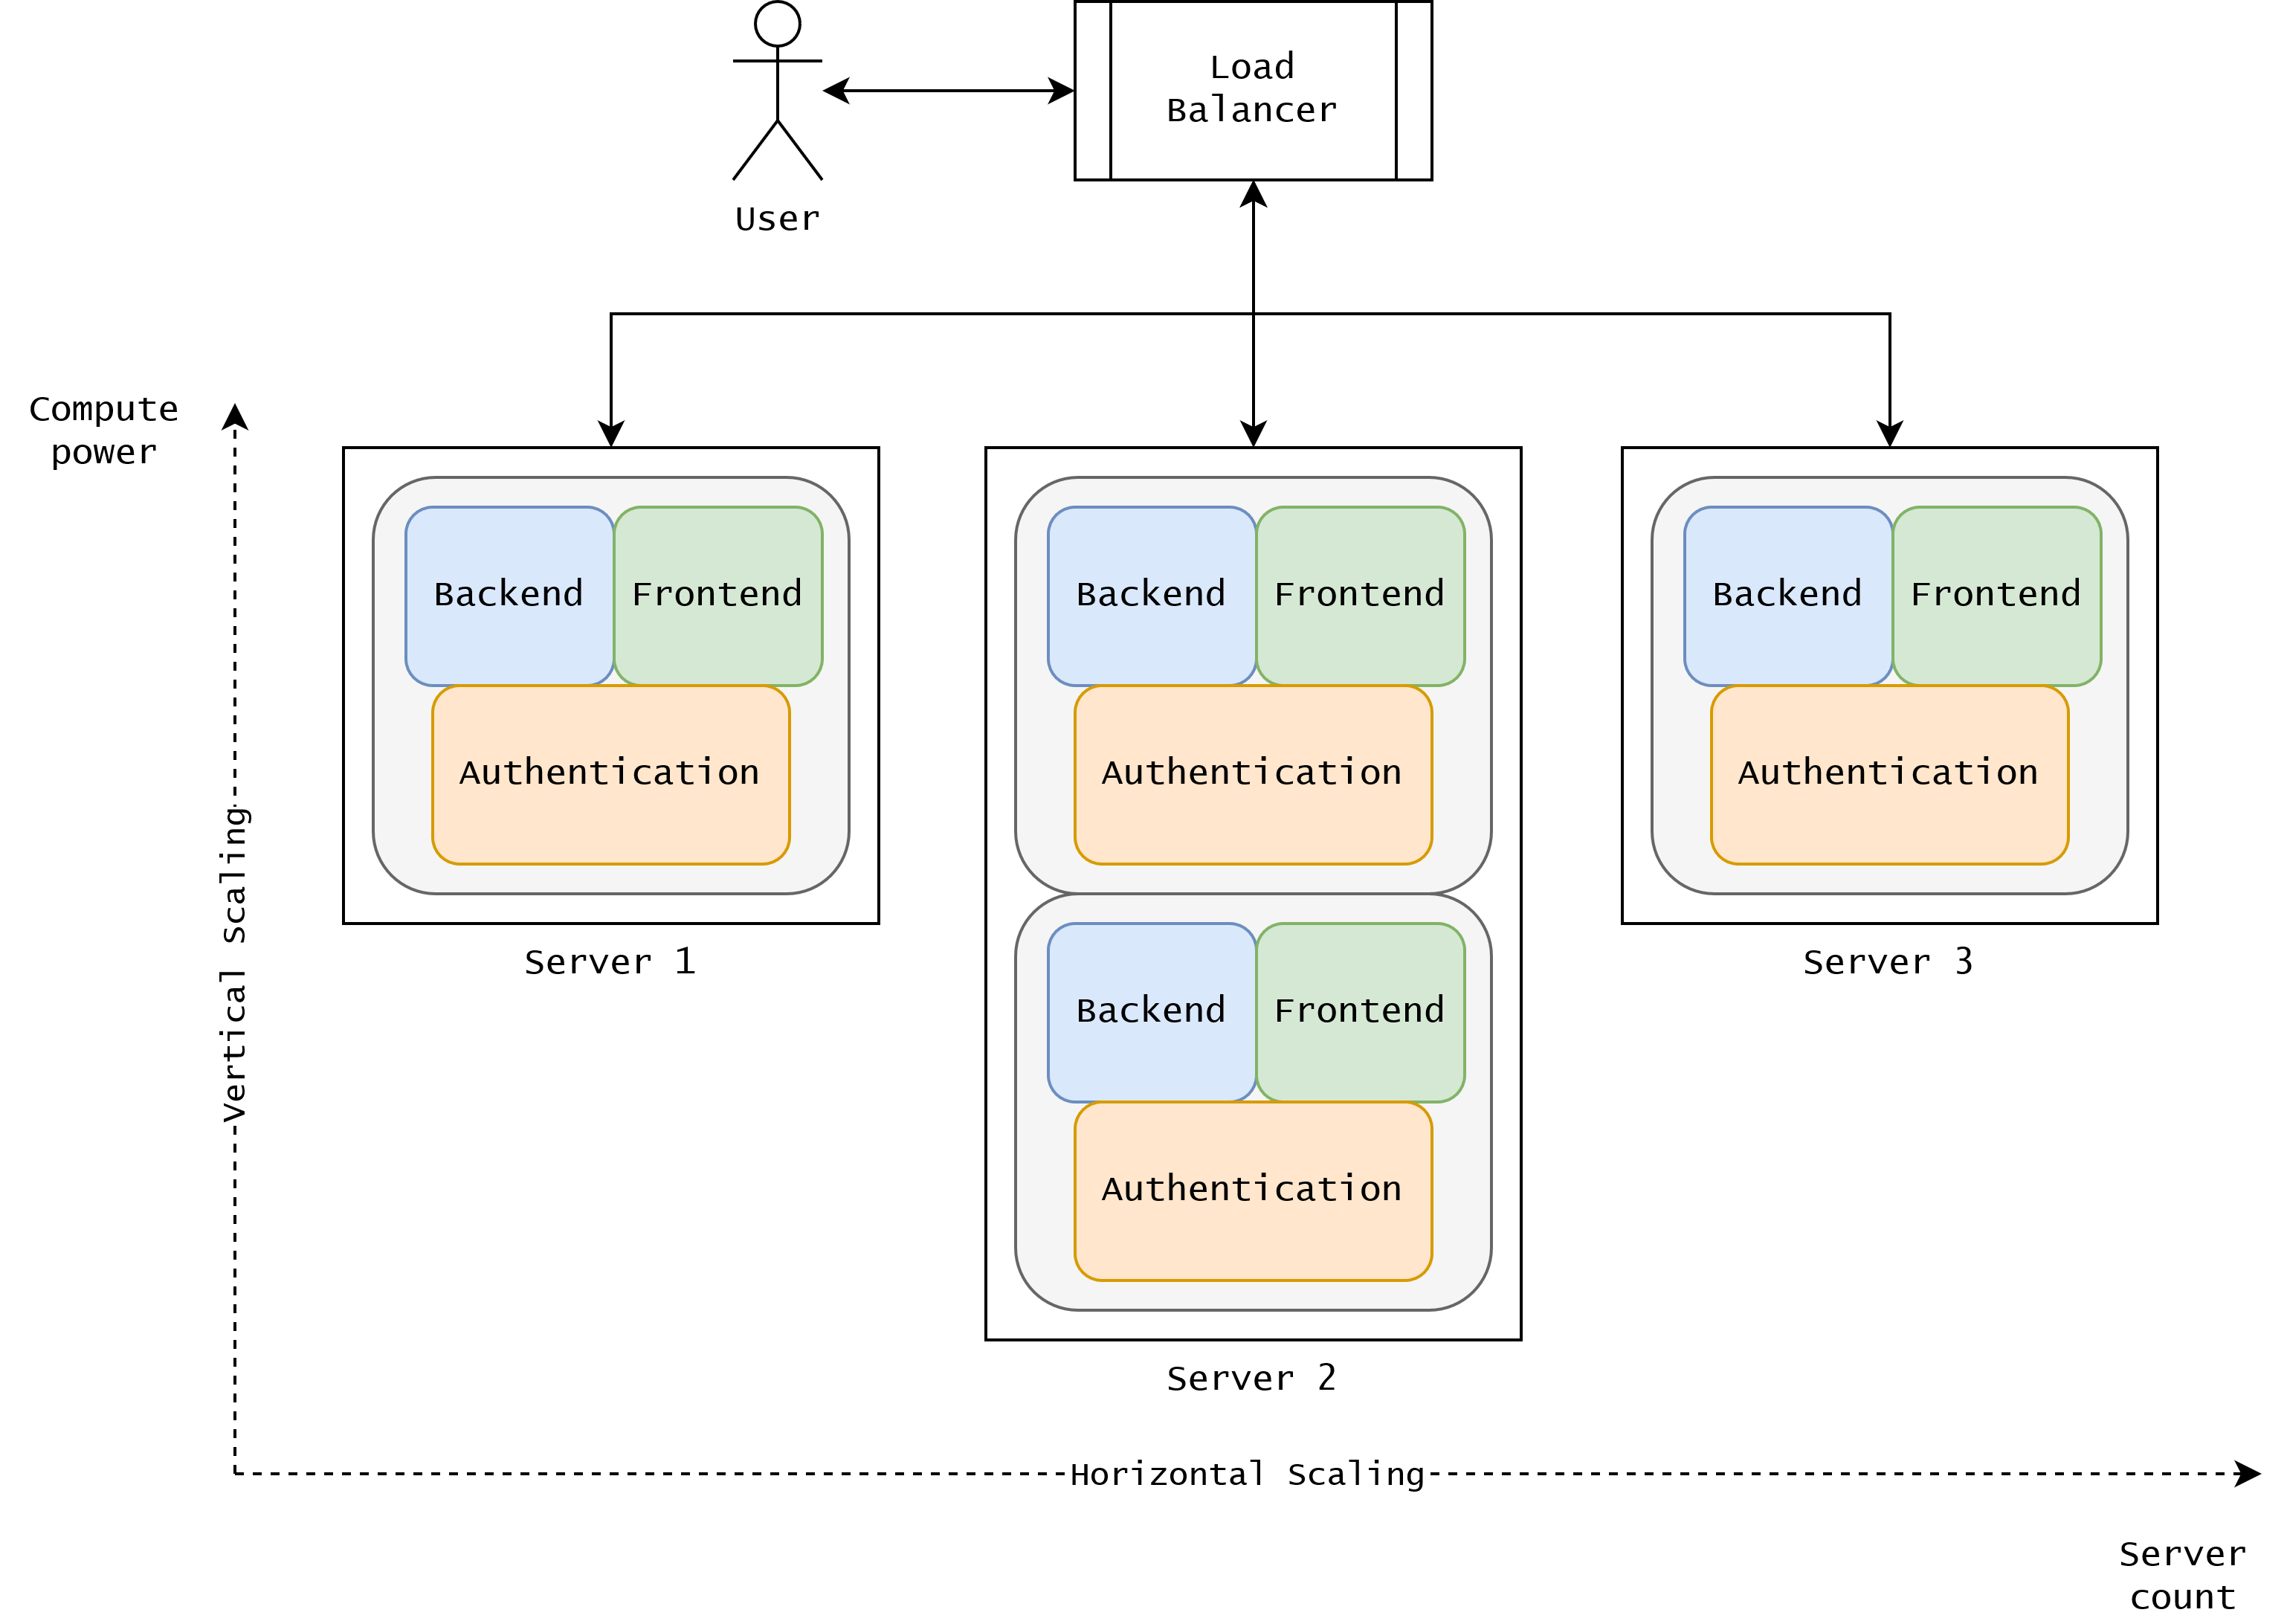
\includegraphics[width=\textwidth]{2_Chapitre2/figures/scaling-monolith.png}
% 	\caption{La mise à l'échelle d'une application à architecture monolithique nécessite de répliquer le monolithe sur plusieurs serveurs.}
% 	\label{figure:context-scaling-monolith}
% \end{figure}

Une application monolithique est construite comme une unité unique, dont les différents services exposés ne sont pas découplés~\cite{villamizarEvaluatingMonolithicMicroservice2015}. Lors de la mise à l'échelle d'un monolithe, l'augmentation du nombre d'instances du monolithe (mise à l'échelle horizontale) peut s'avérer inefficace en termes de coûts, car toutes les parties d'une application ne subissent pas des pics de charge en même temps. Une augmentation des requêtes vers une zone logique de l'application implique une mise à l'échelle de l'infrastructure pour l'ensemble de l'application.
% : dans l'exemple illustré par la figure~\ref{figure:context-scaling-monolith}, une augmentation des requêtes d'authentification implique une mise à l'échelle de l'infrastructure pour l'ensemble de l'application.

% \begin{figure}[!ht]
%     \centering
% 	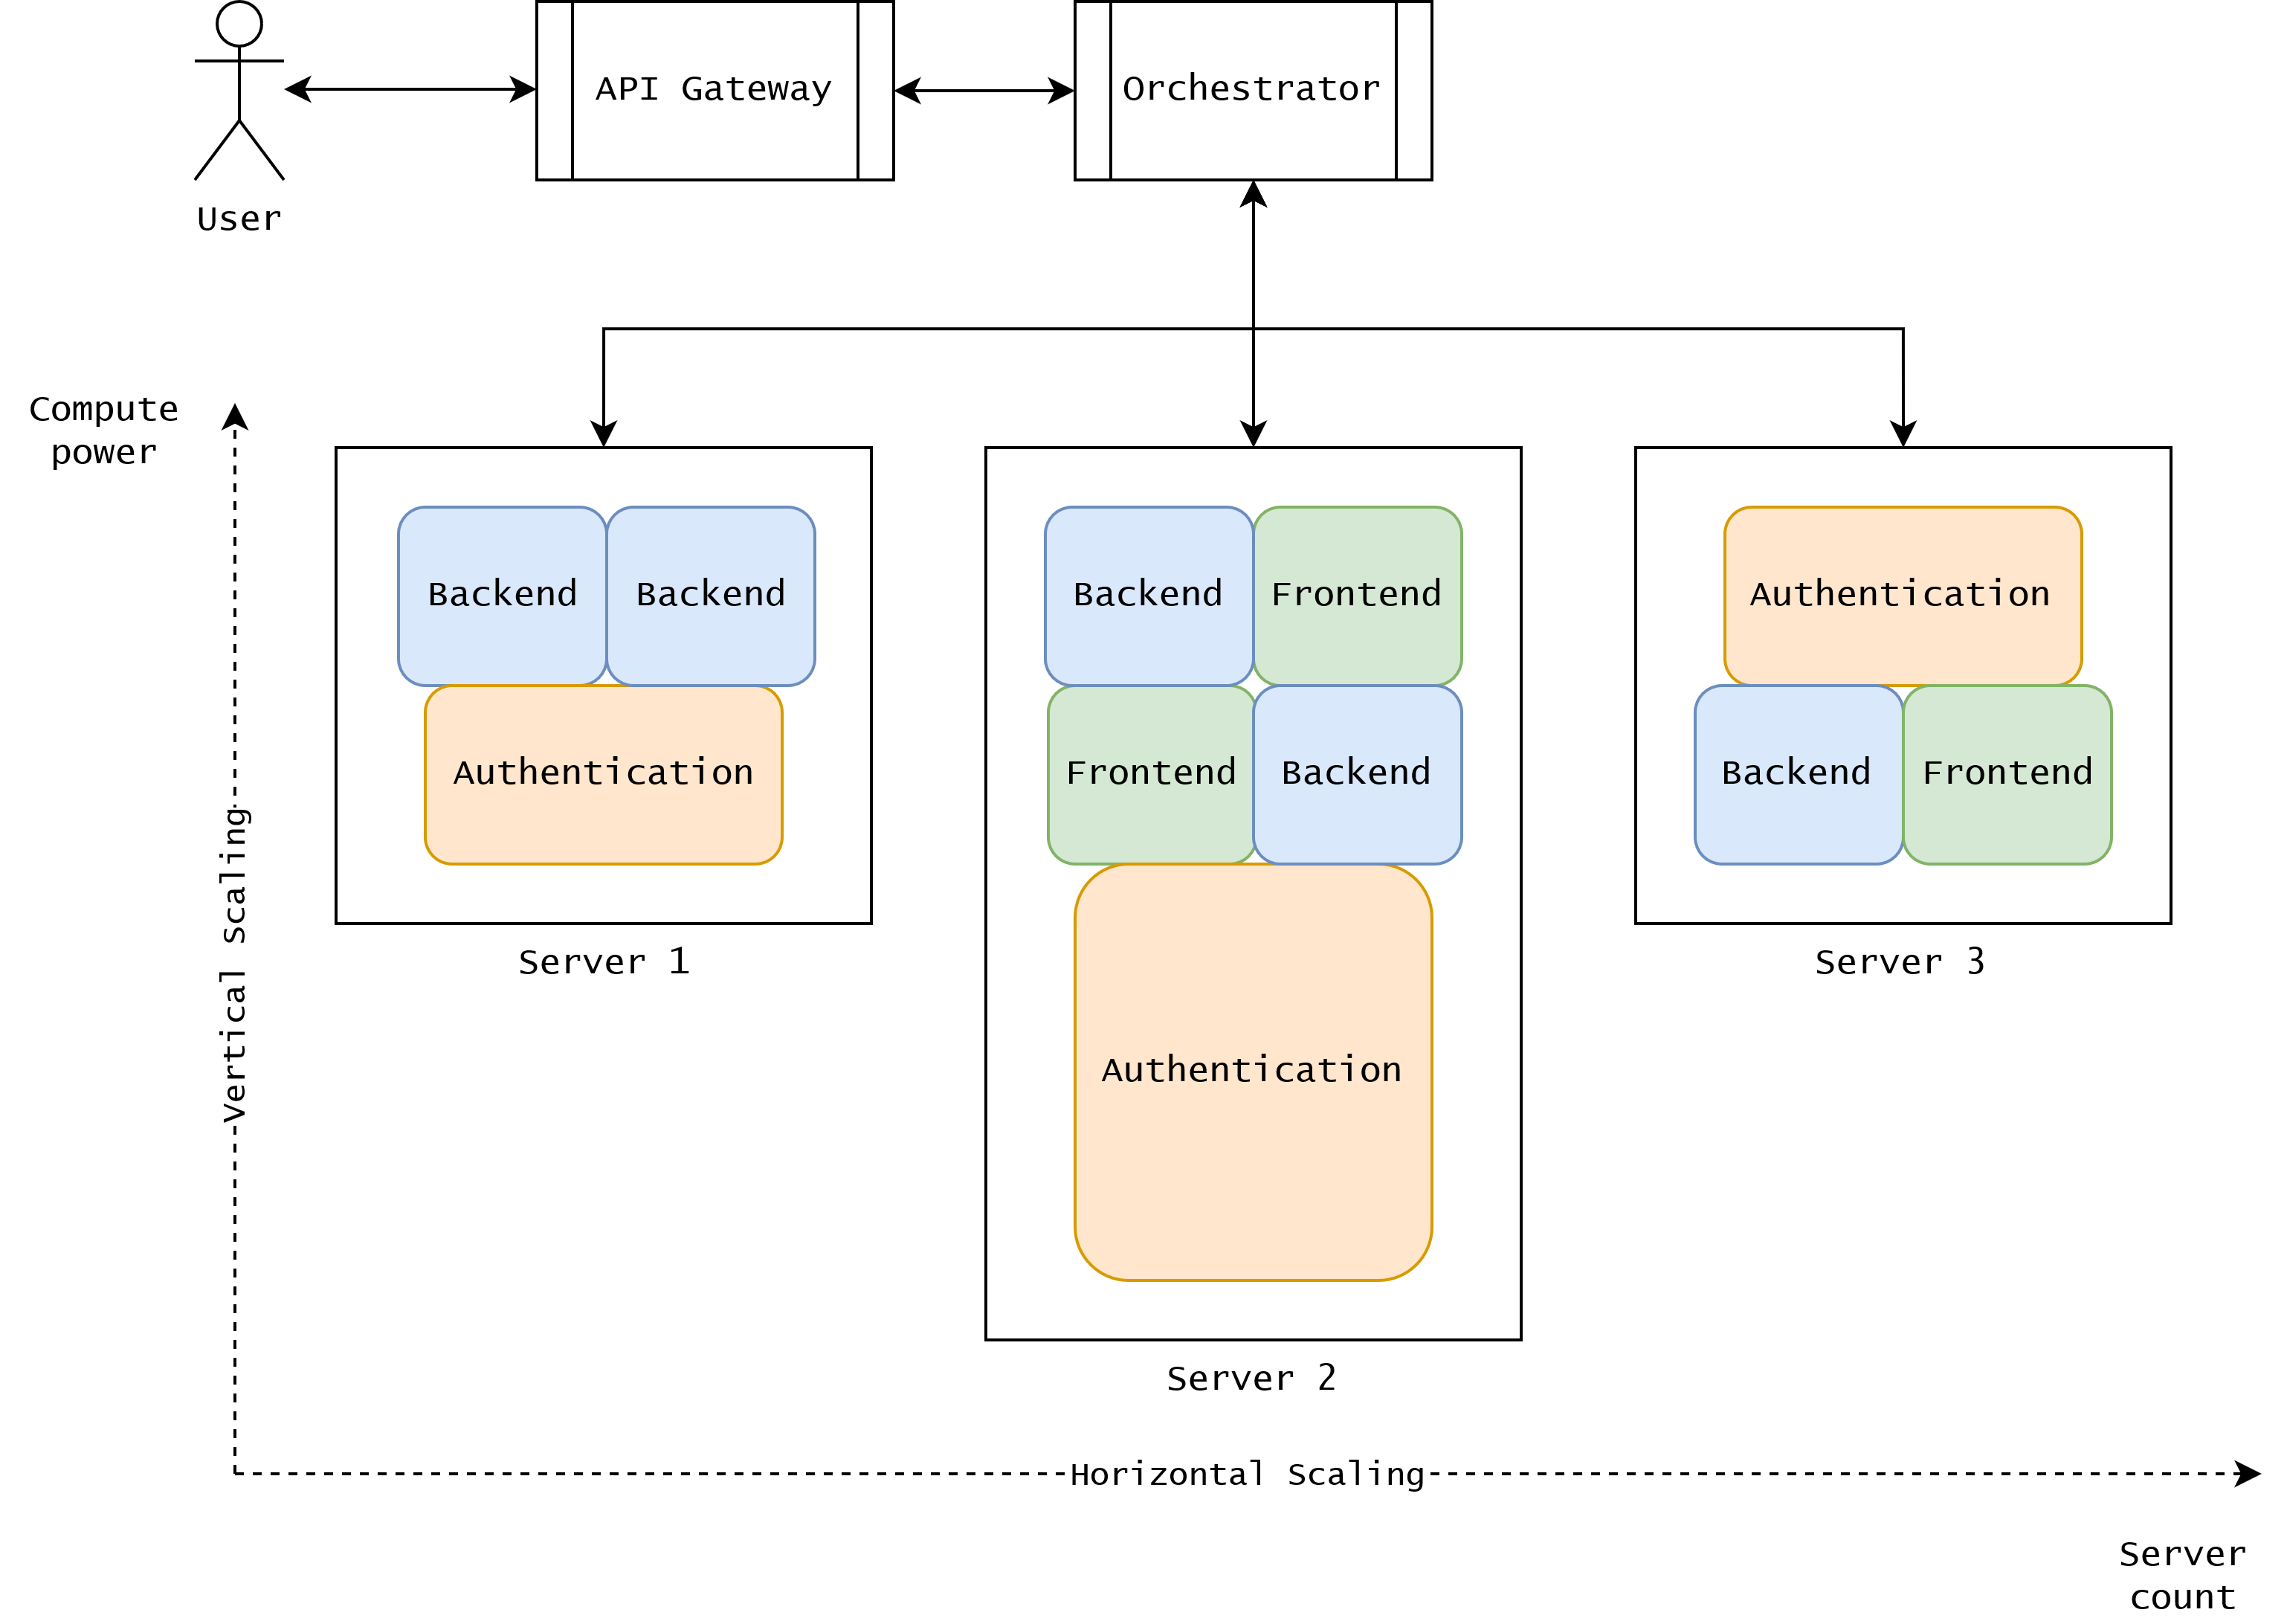
\includegraphics[width=\textwidth]{2_Chapitre2/figures/scaling-microservices.png}
% 	\caption{La mise à l'échelle d'une application architecturée en microservices permet de distribuer et de répliquer chaque microservice de manière indépendante.}
% 	\label{figure:context-scaling-microservices}
% \end{figure}

Une architecture logicielle en microservices consiste à organiser une application sous la forme d'une collection de services faiblement couplés~\cite{12factor}. Chacun de ces services s'exécute dans son propre processus, communique avec les autres par le biais du passage de messages et peut être déployé de manière indépendante sur des serveurs hétérogènes afin d'atteindre les objectifs de niveau de service. Une augmentation des requêtes vers une zone logique de l'application peut être absorbée par la mise à l'échelle de l'infrastructure pour ce seul microservice.
% : dans la figure~\ref{figure:context-scaling-microservices}, une augmentation des requêtes d'authentification peut être absorbée par la mise à l'échelle de l'infrastructure pour le seul microservice d'authentification.

L'infrastructure en microservices facilite donc la mise à l'échelle des applications dans le cloud en permettant un déploiement indépendant pour chacune des composantes d'une application~\cite{vaneykSPECRGReferenceArchitecture2019}.

\subsection{Introduction au modèle serverless}

Dans cette section, nous présentons le modèle de service serverless pour le cloud. Nous passons en revue les caractéristiques essentielles des plateformes serverless, et donnons les propriétés qu'une application doit respecter pour un déploiement serverless.

\subsubsection{Caractéristiques des plateformes serverless}

% TOOD: Le modèle serverless n'est pas une idée nouvelle... Première mention de "serverless" dans la littérature~\cite{andersonServerlessNetworkFile}...

Le serverless désigne à la fois un modèle de programmation et un modèle de service pour le cloud. Dans une architecture serverless, les développeurs conçoivent leurs applications comme une composition de fonctions sans état. Sans état (ou "pur", sans effet de bord) signifie que le résultat du calcul dépend exclusivement des entrées~\cite{burckhardtNetheriteEfficientExecution}. Ces fonctions prennent en entrée une valeur et un contexte d'invocation, et produisent un résultat qui est stocké dans un système de stockage. Leur exécution est déclenchée par un événement tel qu'une requête HTTP, une tâche planifiée, un téléchargement de fichier, etc. Ainsi, le serverless est un modèle dirigé par les événements~\cite{SchleierSmith2021WhatSC}. Dans les offres commerciales de cloud public, le modèle serverless est souvent appelé \textit{Function as a Service}~\cite{hellersteinServerlessComputingOne2019} (\gls{FaaS}).

L'appellation \textit{serverless} ne signifie pas que des serveurs ne sont plus utilisés pour héberger et exécuter des applications. Le terme fait référence à une abstraction sur les ressources matérielles qui permet aux développeurs de s'affranchir de la gestion des serveurs qui supportent leurs applications. Grâce à des mécanismes de mise à l'échelle automatique, les développeurs sont libérés de la réservation des ressources nécessaires au déploiement de leurs charges de travail~\cite{vaneykSPECRGCloud2018}. Les plateformes serverless sont conçues pour gérer de manière automatique les besoins de mise à l'échelle et ainsi répondre aux fluctuations de la demande sur les applications, évitant ainsi aux développeurs d'avoir à définir des stratégies de mise à l'échelle explicites. L'objectif du modèle est de rapprocher les clients de la logique métier de leurs applications~\cite{vaneykSPECRGReferenceArchitecture2019}.

Une caractéristique nouvelle dans le modèle serverless est celui de mise à l'échelle à zéro : lorsqu'une fonction ne reçoit pas de requêtes entrantes, la plateforme serverless libère les ressources qui lui étaient précédemment allouées. Ainsi, les fournisseurs ne facturent les clients que lorsque leur application utilise effectivement des ressources matérielles~\cite{hellersteinServerlessComputingOne2019}.

Pour permettre la mise à l'échelle à zéro des applications, il est nécessaire que celles-ci soient déployées dans des environnements d'exécution "jetables" : leur durée de vie est inférieure à celle des données sur lesquelles ils opèrent. Les données quant à elles doivent être pérennes, et sont donc sauvegardées sur des stockages persistants. On parle de \textit{désagrégation} de l'état des applications. Ainsi, les plateformes serverless dans le cloud public fournissent un ensemble de logiciels dorsaux (ou \textit{backend}), appelés \gls{BaaS}~\cite{mikeroberts2018serverless} (pour \textit{Backend as a Service}). Ce sont des offres commerciales et gérées par le fournisseur, mises à la disposition des développeurs d'applications pour fournir un ensemble de services à longue durée de vie : bases de données, stockage, bus de messages, etc. Ces services tiers constituent l'infrastructure de base des applications serverless.

L'abstraction offerte par le modèle permet aux fournisseurs de déployer le code de leurs clients dans plusieurs zones géographiques. Ce mécanisme de basculement garantit la disponibilité en cas de panne dans une zone de déploiement et réduit le risque de défaillance d'une fonction dans l'application~\cite{taibiPatternsServerlessFunctions2020}. En outre, comme les instances de fonction sont créées à la demande par le fournisseur, le modèle de concurrence offert par les plateformes serverless signifie que les performances d'une application peuvent évoluer linéairement avec le nombre de requêtes~\cite{mcgrathServerlessComputingDesign2017}.

\subsubsection{Caractéristiques des charges de travail serverless}

Du point de vue du client, le serverless permet une mise à l'échelle automatique de leurs applications. La facturation est effectuée au plus juste, uniquement lorsque les ressources sont effectivement utilisées et pour la durée exacte de l'exécution. Du point de vue du fournisseur, la granularité d'allocation permet un meilleur multiplexage des ressources, ce qui se traduit par une efficacité accrue et donc des bénéfices plus importants.

Mais ce mécanisme de mise à l'échelle automatique a un coût en termes de latence : initialiser de nouvelles instances de fonctions pour les requêtes entrantes peut provoquer des délais, menant à des situations où les temps d'initialisation peuvent dominer les temps d'exécution des fonctions~\cite{Jiang2021TowardsDS}. Par ailleurs, les performances peuvent aussi être dégradées en termes de débit : étant donné que l'état des fonctions doit être sauvegardé dans un stockage désagrégé, les applications qui présentent des motifs de communications entre les fonctions peuvent souffrir du temps de récupération des données dans les nœuds de calcul~\cite{mullerLambadaInteractiveData2020}.

En réponse à ces limites du modèle, la Cloud Native Computing Foundation~\footnote{\href{https://www.cncf.io/}{https://www.cncf.io/}} (\gls{CNCF}), une initiative de la Fondation Linux~\footnote{\href{https://www.linuxfoundation.org/}{https://www.linuxfoundation.org/}} soutenue par plus de 800 membres industriels impliqués dans les services cloud, identifie des propriétés idéales pour les cas d'usage serverless, notamment~\cite{cncf2018whitepaper} :

\begin{itemize}
    \item Charges de travail hautement parallèles, asynchrones et concurrentes, avec peu ou pas de communication et pas de synchronisation entre les processus ;
    \item Tâches de fréquence variable, avec de fortes fluctuations de charge, c'est-à-dire des tâches interactives plutôt que des tâches par lots ;
    \item Processus sans état et éphémères, sans besoin majeur d'un temps de démarrage instantané.
\end{itemize}

Pour ces classes d'applications, un déploiement serverless peut être envisagé comme une alternative efficace en matière de coût par rapport aux modèles traditionnels. Toutefois, elles ne recouvrent pas tous les cas d'usage dans le cloud. Si les possibilités de gestion fine des allocations de ressources semblent donner le serverless comme le futur premier modèle de service dans le cloud~\cite{hellersteinServerlessComputingOne2019}, il apparaît donc que les plateformes serverless soulèvent des défis qui restent à relever.

% TODO: Par ailleurs, les utilisateurs déploient des charges de travail très variées sur des plateformes serverless.

\section{Conclusion}

% Dans ce chapitre, nous avons introduit la notion de cloud, les enjeux que de telles plateformes soulèvent en matière d'ordonnancement, et nous avons présenté quelques propriétés d'un modèle de service émergent pour le cloud, le modèle serverless.

Nous avons vu que les offres traditionnelles du cloud reposent sur la réservation de ressources matérielles par les clients. La capacité pour une plateforme à provisionner des ressources à la demande permet aux clients de bénéficier d'une propriété essentielle dans le cloud, l'élasticité. En fonction de la charge (c'est-à-dire le trafic entrant) que subit une application, la plateforme doit permettre d'ajuster la quantité de ressources allouées à l'application, de manière à garantir ses performances.

Cette élasticité n'est généralement pas automatique : il incombe aux clients de faire des prévisions pertinentes dans le cadre de leurs déploiements, et d'ajuster la quantité et la nature des ressources matérielles allouées au plus près de leurs besoins. Cette planification est délicate et une erreur d'estimation peut induire des écarts entre les besoins réels et la capacité allouée. Si les ressources sont surprovisionnées, le client doit supporter un coût financier superflu ; si les estimations sont trop basses, les performances des applications risquent d'en pâtir.

Pour pallier cette limite, un nouveau modèle de service a émergé depuis le milieu des années 2010. Appelé \gls{FaaS}, ou \textit{serverless}, il renverse la responsabilité de l'allocation des ressources dans le cloud. C'est à la plateforme du fournisseur de services d'assigner ces ressources aux applications des clients ou de les libérer, automatiquement, lors de variations de charge. Cela devrait permettre de simplifier la gestion des déploiements pour les clients, tout en autorisant le fournisseur de services à optimiser l'utilisation de ses ressources matérielles.

Si le modèle serverless doit permettre Ce mécanisme n'est pas sans soulever de nouveaux problèmes, notamment en matière de performances. Le chapitre suivant fait état d'un ensemble de défis que les fournisseurs de services doivent relever pour permettre le déploiement d'une variété d'applications sur les plateformes serverless sous contrainte de qualité de service.


\clearemptydoublepage
\chapter{Serverless, allocation et placement dynamiques dans le cloud : État de l'art}
\label{chapter:sota}

TODO: Première mention de "serverless" dans la littérature~\cite{andersonServerlessNetworkFile}

TODO: Autoscaling = problème non résulé~\cite{straesserWhyItNot2022}

\section{Serverless : caractéristiques et écosystème}

Le modèle serverless constitue un changement de paradigme dans le cloud public : par opposition aux modèles traditionnels, les clients serverless ne réservent pas de ressources matérielles. L'exécution de leur code est dirigée par des événements (requêtes HTTP, tâches programmées, etc.) et la facturation s'effectue sur la base de l'usage réel des ressources. En contrepartie, la responsabilité de l'allocation des ressources et du placement des tâches incombe au fournisseur.

Malgré une tarification attractive avec des plans gratuits étendus dans les offres commerciales, et un panel varié de solutions open source ciblant les principaux orchestrateurs de cloud, le FaaS n'est pas encore devenu le modèle d'abonnement au cloud de référence : certains défis sont encore ouverts et doivent être relevés avant que le serverless ne devienne omniprésent.

Un véritable défi pour remédier à ces lacunes est d'éviter les solutions "serveurful" au problème de l'allocation dynamique des ressources, c'est-à-dire l'allocation de ressources stables supplémentaires qui ne s'étendent volontairement pas jusqu'à zéro~\cite{hellersteinServerlessComputingOne2019}.

Le serverless est un sujet animé dans le domaine du cloud computing et de nombreux auteurs contribuent à atténuer ces revers : le nombre d'articles publiés autour du serverless a presque doublé entre 2019 et 2020~\cite{hassanSurveyServerlessComputing2021}.

\subsection{Description de l'offre serverless}

Dans cette première sous-section, nous proposons un tour d'horizon des différentes offres serverless chez les fournisseurs de cloud public, ainsi que des solutions open source disponibles pour le cloud privé.

Le tableau~\ref{table:commercial-faas} présente un sommaire des offres commerciales FaaS dans le cloud public, leurs modèles de tarifications ainsi que certaines de leurs caractéristiques. Ce sommaire inclut Alibaba Function Compute~\cite{alibaba-function-compute}, Amazon Web Services Lambda~\cite{aws-lambda}, Microsoft Azure Functions~\cite{azure-functions}, Google Cloud Functions~\cite{google-cloud-functions}, IBM Cloud Functions~\cite{ibm-cloud-functions} et Oracle Cloud Functions~\cite{oracle-cloud-functions}.

Le tableau~\ref{table:foss-faas} présente ensuite quelques solutions majeures disponibles dans la communauté open source, et donne un aperçu de l'état du projet en fonction de son adoption par les utilisateurs et la quantité de contributions, ainsi que les partenaires industriels qui accompagnent le projet. On y trouve Apache OpenWhisk~\cite{openwhisk}, Fission~\cite{fission}, Fn~\cite{fn}, Knative~\cite{knative} et OpenFaaS~\cite{openfaas}.

\subsubsection{Solutions commerciales dans le cloud public}

Pour positionner chacune des offres commerciales, nous avons choisi de les comparer sur la base des critères suivants :

\begin{itemize}
    \item Modèle de tarification : les modalités selon lesquelles les clients peuvent anticiper le coût de leurs déploiements dans le cadre d'une offre serverless dans le cloud public ;
    \item Caractéristiques : les limites imposées par le fournisseur de services en matière d'utilisation et de disponibilité des ressources.
\end{itemize}

TODO: refaire le tableau

% \begin{longtblr}[
%     caption = {Cloud customers are faced with a diversity of FaaS offerings},
%     label = {table:commercial-faas},
%     note{a} = {billed per \num{10000} requests (for USD 0.02)}
% ]{
%     rowhead = 3,
%     colspec = { X[l,1.8] X[2,l]X[2,l] X[l]X[l]X[l]X[1.8,l] },
%     row{1-2} = { l, font = {\bfseries} },
%     row{3} = { b, font = \footnotesize%, cmd={\rotatebox{60}}
%                 },
%     row{4-Z} = { m, font = \footnotesize, rowsep = 1ex },
%     column{1} = { font = {\bfseries}}
% }

% \toprule
% \SetCell[r=3]{m} Service & \SetCell[c=2]{c} Pricing model && \SetCell[c=4]{c} Properties \\
% \cmidrule[lr=-0.4]{2-3}
% \cmidrule[lr=-0.4]{4-7}
% &
% free quota per month &
% pay-as-you-go cost &
% \\
% &
% \# of invocations / compute resources [\unit{\giga\byte\second}]&
% \num{1}M requests / \qty{1}{\giga\byte\second} compute [USD]&
% code size &
% memory &
% execution time &
% payload size \\
% \midrule


% Alibaba Function Compute &
% \num{1000000} / \num{400000} &
% \num{20}\TblrNote{a} / \num{0.000016384} &
% \qty{500}{\mega\byte} &
% \qty{3}{\giga\byte}&
% \qty{24}{\hour} &
% \qty{128}{\kilo\byte} (request), \qty{6}{\mega\byte} (response)
% \\

% AWS Lambda &
% \num{1000000} / \num{400000} &
% \num{0.2} / \num{0.0000166667} &
% \qty{10}{\giga\byte}&
% \qty{10240}{\mega\byte} &
% \qty{15}{\minute} &
% \qty{6}{\mega\byte} (synchronous), \qty{256}{\kilo\byte} (asynchronous) for requests and responses
% \\

% Azure Functions &
% \num{1000000} / \num{400000} &
% \num{0.2} / \num{0.000016} &
% N/A &
% \qty{1.5}{\giga\byte} &
% \qty{10}{\minute}&
% \qty{100}{\mega\byte} (request)
% \\

% Google Cloud Functions   &
% \num{2000000} / \num{400000} &
% \num{0.4} / \num{0.0000025} &
% \qty{500}{\mega\byte}&
% \qty{8}{\giga\byte}&
% \qty{9}{\minute}&
% \qty{10}{\mega\byte} for requests and responses
% \\

% IBM Cloud Functions  &
% \num{5000000} / \num{400000} &
% N/A / \num{0.000017} &
% \qty{48}{\mega\byte} &
% \qty{2048}{\mega\byte} &
% \qty{60}{\second} &
% \qty{5}{\mega\byte} for requests and responses
% \\

% Oracle Cloud Functions &
% \num{2000000} / \num{400000} &
% \num{0.2} / \num{0.00001417} &
% N/A &
% \qty{2048}{\mega\byte} &
% \qty{5}{\minute}&
% \qty{6}{\mega\byte}
% \\

% \bottomrule
% \end{longtblr}

\subsubsection{Solution open source pour le cloud privé}

Comme mesure de l'état d'un projet ainsi que de son adoption, nous choisissons deux indicateurs disponibles publiquement sur les dépôts GitHub~\cite{github} :

\begin{itemize}
    \item Les "GitHub stars" (ou étoiles) indiquent combien d'utilisateurs de GitHub ont choisi de s'abonner aux mises à jour d'un projet ;
    \item Nous considérons comme contributeurs les utilisateurs ayant publié dix, ou plus de dix modifications au code source (\textit{git commits}) du projet.
\end{itemize}

\begin{table}[H]
\caption{Open source solutions allow cloud providers to devise their own FaaS offering}
\centering
\begin{tabularx}{\textwidth} { 
  | >{\centering\arraybackslash}X 
  | >{\centering\arraybackslash}X 
  | >{\centering\arraybackslash}X  | }
\hline
                       & \textbf{Project status and adoption} & \textbf{Corporate backer} \\ \hline
Apache OpenWhisk       & 5.8k GitHub stars, 34 contributors ($\geq$ 10 commits) & IBM (Apache Foundation)             \\ \hline
Fission                & 7.3k GitHub stars, 10 contributors ($\geq$ 10 commits) & Platform9             \\ \hline
Fn                     & 5.3k GitHub stars, 21 contributors ($\geq$ 10 commits) & Oracle             \\ \hline
Knative                & 4.5k GitHub stars, 55 contributors ($\geq$ 10 commits) & Google             \\ \hline
OpenFaaS               & 22.2k GitHub stars, 13 contributors ($\geq$ 10 commits) & VMware             \\ \hline
\end{tabularx}
\label{table:foss-faas}
\end{table}

\section{Le défi de l'allocation dynamique des ressources}

\subsection{Délais et fréquence du démarrage à froid}
\label{sota-cold-start}

Comme les conteneurs serverless doivent passer un minimum de temps dans un état d'inactivité, ils sont mis en marche et arrêtés très fréquemment par rapport aux conteneurs PaaS ou aux VM IaaS. Chaque fois qu'une fonction est appelée et doit être mise à l'échelle à partir de zéro, le conteneur ou la machine virtuelle hébergeant le code de la fonction doit passer par sa phase d'initialisation : c'est ce qu'on appelle un "cold start"~\cite{lloydImprovingApplicationMigration2018}, ou "démarrage à froid". Les démarrages à froid peuvent entraîner des pénalités de latence, aggravées par les retards qui font boule de neige lors de la composition des fonctions dans le contexte d'applications complexes~\cite{mohanAgileColdStartsa}.

Les fonctions sont généralement invoquées en rafales - le modèle d'exécution AWS Lambda peut maximiser la concurrence en instanciant une fonction dans des centaines, voire des milliers de bacs à sable répartis sur différents sites géographiques~\cite{aws-lambda-scaling}. Quelques minutes après avoir traité une requête, le sandbox d'une fonction est libéré du nœud d'exécution ; de plus, les futures nouvelles instances ne sont pas garanties d'être créées sur le même nœud. Cela conduit à des situations dans lesquelles l'environnement d'une fonction n'est pas mis en cache sur le nœud. Le code et les bibliothèques associées doivent être récupérés et copiés à nouveau sur le système de fichiers, ce qui entraîne une latence de démarrage à froid.

Une approche "naïve" consisterait à pré-allouer des ressources matérielles afin de maintenir un pool de conteneurs de fonctions prêt à recevoir de nouvelles requêtes. Cette approche n'est pas acceptable car elle s'éloigne de la possibilité d'une mise à l'échelle à zéro.

Vahidinia et al.~\cite{vahidiniaColdStartServerless2020} proposent une étude complète de la position et des stratégies de diverses offres commerciales FaaS concernant le démarrage à froid. Alors que l'informatique sans serveur suggère de faire tourner des instances jetables de fonctions pour traiter chaque requête entrante, les auteurs notent que les acteurs commerciaux tels qu'AWS, Google et Microsoft réutilisent tous dans une certaine mesure les bacs à sable d'exécution, en les maintenant en activité pendant une période de temporisation afin de contourner les coûts de latence induits par les démarrages à froid.

\subsubsection{Réduire les temps d'initialisation}

Différentes approches peuvent être mises en œuvre par les fournisseurs de services en nuage pour réduire le temps d'initialisation des bacs à sable de fonctions. Il s'agit d'un travail crucial car les invocations de fonctions suivent des modèles généralement imprévisibles~\cite{shahradServerlessWildCharacterizing}. Cette section explore les contributions de la littérature qui se concentrent sur la réduction de l'écart de latence entre les modèles serverless et serverful.

\textbf{Approche d'optimisation en bac à sable}

Dans~\cite{mullerLambadaInteractiveData2020}, les auteurs proposent Lambada pour résoudre le problème du démarrage à froid dans le contexte de l'analyse des données distribuées en mettant en lots l'invocation des travailleurs en parallèle. Ils identifient un goulot d'étranglement dans le processus d'invocation de nouveaux travailleurs : dans leur évaluation, ils montrent que l'invocation de 1000 travailleurs AWS Lambda prend entre 3,4 et 4,4 secondes. Dans leur contribution, chaque travailleur est responsable de l'invocation d'une deuxième génération de bacs à sable, qui invoqueront à leur tour une génération suivante de travailleurs jusqu'à ce que le processus de mise à l'échelle soit terminé. Cette technique permet de créer plusieurs milliers de travailleurs en moins de 4 secondes.

Dans~\cite{mancoMyVMLighter2017}, les auteurs proposent LightVM pour mettre le temps de démarrage des VM au même niveau que les conteneurs. Les auteurs montrent que les temps d'instanciation augmentent linéairement avec la taille de l'image : la création d'un environnement sandbox pour l'exécution d'une application est une opération liée aux entrées-sorties. En repensant le plan de contrôle de Xen et en utilisant des VM légères qui incluent un environnement minimal nécessaire à l'exécution de l'application en bac à sable, ils obtiennent des temps de démarrage comparables aux performances de la mise en œuvre de \texttt{fork}/\texttt{exec} dans Linux.

Dans~\cite{akkusSANDHighPerformanceServerless}, les auteurs proposent que des mécanismes d'isolation complets tels que les conteneurs soient nécessaires pour isoler les charges de travail entre les clients, alors qu'à la granularité d'une application unique, les processus suffisent à isoler les fonctions. Dans SAND, ils mettent en œuvre un mécanisme d'isolation au-dessus de Docker qui permet des interactions efficaces en termes de ressources, élastiques et à faible latence entre les fonctions.

Dans~\cite{agacheFirecrackerLightweightVirtualization}, les auteurs présentent Firecracker, qui s'est développé pour devenir la technologie de virtualisation \textit{de facto} pour serverless, utilisée chez AWS Lambda. Ils s'attaquent au compromis isolation versus performances en introduisant des VM légères (ou MicroVM) à la place des conteneurs comme mécanisme de sandboxing pour les charges de travail serverless. Firecracker atteint des temps de démarrage inférieurs à 125 ms en remplaçant QEMU par une implémentation personnalisée d'un moniteur de machine virtuelle qui s'exécute au-dessus de KVM et permet de créer jusqu'à 150 MicroVM par seconde et par hôte avec une surcharge de mémoire de 3\%.

\textbf{Approche "snaptshotting"} \label{sota-snapshotting}

Dans~\cite{duCatalyzerSubmillisecondStartup2020}, les auteurs affirment que la surcharge de démarrage dans les bacs à sable basés sur la virtualisation est due à leur nature agnostique vis-à-vis des applications. En effet, ils montrent que la latence d'initialisation de l'application domine la latence de démarrage totale. Dans Catalyzer, les auteurs montrent que les instances de bac à sable d'une même fonction possèdent des états d'initialisation très similaires, et présentent donc une solution d'instantané qui permet de restaurer une instance de fonction à partir d'une image de point de contrôle, en sautant effectivement la phase d'initialisation de l'application lors d'une mise à l'échelle à partir de zéro. Ils construisent une solution basée sur le gVisor de Google~\cite{gvisor} qui surpasse systématiquement les technologies de pointe telles que Firecracker\cite{agacheFirecrackerLightweightVirtualization}, HyperContainer et Docker d'un ordre de grandeur.

Dans~\cite{ustiugovBenchmarkingAnalysisOptimization2021}, les auteurs présentent vHive, un cadre d'analyse comparative pour l'expérimentation serverless qui leur permet de montrer qu'une latence élevée peut être attribuée à des défauts de page fréquents pendant l'initialisation des bacs à sable, avec des modèles très similaires entre les exécutions d'une même fonction -- 97\% des pages mémoire étant identiques entre les invocations des fonctions étudiées. Les auteurs proposent REAP pour créer des images de la configuration de la mémoire d'un bac à sable qui permettent de prélever des pages du disque vers la mémoire, de remplir rapidement la mémoire d'invité avant l'exécution de la fonction et d'éviter ainsi la majorité des erreurs de page au moment de l'initialisation. Cette technique permet d'accélérer le délai de démarrage à froid de 3,7 fois en moyenne.

Dans~\cite{shillakerFaasmLightweightIsolation2020}, les auteurs proposent Faaslets, un nouveau mécanisme d'isolation basé sur l'isolation des fautes logicielles fournie par WebAssembly. Les faaslets permettent de restaurer l'état d'une fonction à partir d'instantanés déjà initialisés. Ces snapshots sont pré-initialisés à l'avance et peuvent être restaurés en quelques centaines de millisecondes, même d'un hôte à l'autre. Les fasslets tirent parti du modèle de mémoire de WebAssembly : les tableaux d'octets linéaires peuvent être copiés sans une longue phase de (dé)sérialisation.

\textbf{Approche de la mise en cache}

Dans~\cite{oakesSOCKRapidTask}, les auteurs soutiennent que si le serverless permet de réaliser des économies grâce à une élasticité accrue et à la vélocité des développeurs, les longs temps d'initialisation des conteneurs nuisent aux performances de latence des applications déployées. Ils identifient des goulets d'étranglement dans les primitives Linux impliquées dans l'initialisation des conteneurs, les dépendances des paquets étant le principal coupable des opérations d'E/S pendant le sandboxing. Ils proposent SOCK comme un système de conteneurs optimisé pour les tâches serverless qui s'appuie sur OpenLambda et repose sur un système de mise en cache conscient des paquets, et montrent que leur solution offre des accélérations jusqu'à 21 fois par rapport à Docker.

Dans~\cite{fuerstFaasCacheKeepingServerless2021}, l'auteur montre des similitudes conceptuelles entre la mise en cache d'objets et la fonction keep-alive, ce qui leur permet de concevoir des politiques qui réduisent les délais de démarrage à froid. En s'appuyant sur cette analogie, ils proposent une politique de maintien en vie qui est essentiellement une politique de terminaison (ou d'éviction) de fonction. En gardant les fonctions chaudes aussi longtemps que possible (c'est-à-dire aussi longtemps que les ressources du serveur le permettent), FaasCache parvient à doubler le nombre de requêtes pouvant être traitées dans sa mise en œuvre basée sur OpenWhisk.
\\

La capacité des plateformes serverless à mettre à l'échelle une fonction jusqu'à zéro réplique afin d'éviter de facturer les clients pour les ressources inactives est une différence clé par rapport aux modèles de services cloud traditionnels. La recherche de techniques qui minimisent l'impact d'un démarrage à froid sur la latence de la fonction est un sujet de recherche essentiel, car les temps d'initialisation prohibitifs entravent le potentiel des plateformes FaaS à concurrencer les plateformes PaaS.

\subsection{Hétérogénéité du matériel}

Les clients de l'informatique en nuage sont censés réserver différentes ressources en fonction des besoins de leurs applications, qu'il s'agisse d'une architecture CPU spécifique, d'accélérateurs matériels, d'un stockage ad hoc, etc. Un exemple frappant est celui de l'apprentissage automatique distribué, dans lequel de nombreux GPU sont utilisés pour accélérer l'apprentissage des modèles - en outre, les fournisseurs de cloud commencent à généraliser l'accès au matériel spécialisé tel que les TPU dans les VM.

La sélection manuelle des ressources matérielles (" type d'instance "), attendue des clients dans les offres IaaS comme Amazon EC2, n'a pas de sens dans le paradigme serverless. L'accélération matérielle devrait être décidée par le fournisseur par application ou par requête. À ce jour, cette possibilité n'est pas disponible dans les offres FaaS telles qu'AWS Lambda.

Dans~\cite{Jiang2021TowardsDS}, les auteurs ont entrepris de comparer les configurations IaaS et FaaS pour la formation à l'apprentissage automatique sur les offres Amazon Web Services (resp. EC2 et Lambda). Ils proposent une implémentation de l'apprentissage basée sur le FaaS, LambdaML, et la comparent à des frameworks de l'état de l'art s'exécutant sur des instances EC2. Ils ont mesuré que l'apprentissage serverless peut être rentable tant que le modèle converge suffisamment rapidement pour que les communications inter-fonctions ne dominent pas le temps d'exécution total. Dans le cas contraire, une configuration IaaS utilisant des GPU sera plus performante que n'importe quelle configuration FaaS, offrant de meilleures performances tout en étant plus rentable.

Dans~\cite{bacisBlastFunctionFPGAasaServiceSystem2020}, les auteurs explorent le multitenancy dans les FPGA pour atteindre un taux d'utilisation plus élevé de la carte. Ils proposent BlastFunction, un système évolutif pour le partage de temps FPGA dans un contexte serverless. Leur mise en œuvre repose sur trois éléments de base : une bibliothèque qui permet un accès transparent aux dispositifs partagés à distance, un plan de contrôle distribué qui surveille les FPGA pour réaliser le partage du temps, et un registre central qui gère l'allocation des cartes à chaque nœud de calcul. Cette conception permet d'atteindre des taux d'utilisation plus élevés sur les cartes et donc de traiter un plus grand nombre de requêtes, en particulier en cas de charge élevée, bien qu'au prix d'une augmentation de 36% de la latence en raison de la concurrence supplémentaire.

Dans~\cite{diamantopoulosAccelerationasauServiceCloudnativeMonteCarlo2021}, les auteurs se concentrent sur un cas d'utilisation des services financiers et proposent des FPGA pour réduire le temps de réponse de bout en bout et augmenter l'évolutivité dans une architecture microservices. L'application étudiée est à forte intensité de calcul et présente des caractéristiques de temps réel. Ils proposent CloudiFi, un cadre cloud-native qui expose les accélérateurs matériels en tant que microservices par le biais d'une API HTTP RESTful. CloudiFi permet de décharger les charges de travail sur les accélérateurs matériels au niveau des fonctions. Une évaluation des performances de l'application sous CloudiFi montre des gains de temps de réponse de 485x lors de l'utilisation de FPGA connectés au réseau par rapport à une configuration vanille.

Les CPU ARM et RISC, les GPU et les FPGA sont de plus en plus utilisés dans les centres de données pour répondre à la demande de performance, d'efficacité énergétique et de facteur de forme réduit. Dans~\cite{hortaXartrekRuntimeExecution2021}, les auteurs soutiennent que, puisque ces plateformes d'exécution hétérogènes sont généralement colocalisées avec un processeur hôte général, la possibilité de tirer parti de leurs caractéristiques en migrant les charges de travail pourrait entraîner des gains de performance significatifs. Ils proposent Xar-Trek, un compilateur et un moniteur d'exécution pour permettre la migration de l'exécution à travers les CPU et FPGA hétérogènes-ISA selon une politique d'ordonnanceur. Xar-Trek implique un effort de programmation limité : l'application est écrite une seule fois et compilée pour différentes cibles grâce à la chaîne d'outils Xilinx, sans annotations de synthèse de haut niveau nécessaires pour guider le compilateur. Le système d'exécution de Xar-Trek, un ordonnanceur en ligne dans l'espace utilisateur, est capable de déterminer si une migration est efficace et de procéder à la migration des fonctions sélectionnées qui bénéficient le plus de l'accélération. L'évaluation des charges de travail de vision industrielle et de calcul intensif révèle que tant que les charges de travail sont dominées par des fonctions à forte intensité de calcul, Xar-Trek est toujours plus performant que les configurations vanille, avec des gains de performance compris entre 26 et 32 %.

Même lorsque du matériel hétérogène est installé sur le même nœud, il est généralement interconnecté par des bus PCI-Express gérés par l'unité centrale de l'hôte. Les communications sont réalisées à l'aide d'interfaces de passage de messages qui introduisent des coûts de bande passante et de latence. Dans~\cite{vilanovaSlashingDisaggregationTax2022}, les auteurs présentent FractOS, un système d'exploitation distribué pour les centres de données hétérogènes et désagrégés. FractOS permet de décentraliser l'exécution des applications : au lieu de s'appuyer sur l'unité centrale pour transmettre le contrôle et les données d'une plate-forme d'exécution à l'autre, FractOS fournit aux applications une bibliothèque qui permet des communications directes entre les appareils, grâce à un contrôleur sous-jacent qui capte les appels système et fournit des fonctionnalités directes d'appareil à appareil. Lorsqu'elle a été testée sur une application de vérification des visages qui exploite les GPU pour accélérer les calculs, leur solution a permis d'accélérer le temps d'exécution de 47 % et de diviser le trafic réseau global par 3.
\\

Avec la progression exponentielle et l'intérêt croissant dans le domaine de l'apprentissage automatique, la demande d'accélérateurs matériels dans le cloud n'a jamais été aussi importante. Les offres commerciales serverless sont à la traîne des IaaS traditionnels à cet égard, car aucune n'offre d'accès aux GPU, TPU ni FPGA. En outre, l'allocation dynamique de ce type de matériel pour accélérer des tâches sélectionnées offre aux fournisseurs la possibilité d'améliorer leur utilisation des ressources et leur consommation d'énergie.

\section{Ordonnancer et placer les requêtes utilisateur}

\subsection{Communication des données} \label{sota-communications}

Dans les offres FaaS, les fonctions ne sont pas adressables : la composition se fait par le stockage des résultats dans un niveau de stockage lent avec état qui n'est généralement pas colocalisé avec le niveau de calcul.

Comme les fonctions d'une même application ne peuvent pas partager la mémoire ou les descripteurs de fichiers pour réaliser l'IPC, elles doivent établir la communication par le biais d'interfaces de passage de messages, ce qui introduit une surcharge lorsque les données doivent circuler à travers l'application.

Ce problème est particulièrement préoccupant lorsque des applications gourmandes en données doivent travailler avec des données froides, c'est-à-dire des données auxquelles on accède peu et qui ne sont donc pas mises en cache, et qui sont stockées sur des supports moins performants tels que des disques durs situés sur des nœuds distants. Dans~\cite{Jiang2021TowardsDS}, les auteurs présentent LambdaML, une plateforme d'analyse comparative qui permet de comparer les performances de l'apprentissage distribué de modèles de machine entre les offres IaaS et FaaS. Ils constatent que l'utilisation de FaaS pour la formation à l'apprentissage machine peut être rentable tant que les modèles présentent des schémas de communication réduits.

Dans~\cite{mullerLambadaInteractiveData2020}, les auteurs montrent que FaaS peut être rentable lors de l'exécution de requêtes interactives sporadiques sur des gigaoctets à un téraoctet de données froides. En fournissant des opérateurs de données serverless avec Lambada, ils réalisent des requêtes interactives sur plus de 1 TB de données stockées sur Amazon S3 en approximativement 15 secondes, ce qui est dans le même parc à balles que les solutions commerciales Query-as-a-Service.

Dans~\cite{Romero2021FaaTAT}, les auteurs soutiennent que les offres serverless manquent d'une couche de mise en cache des données en mémoire et par application qui permettrait une mise à l'échelle automatique et fonctionnerait de manière transparente. Faa\$T peut former une couche de mise en cache distribuée fortement cohérente lorsque plusieurs instances d'une application sont lancées, le dernier nœud de mise en cache disparaissant lorsque l'application est réduite à zéro, ce qui permet de facturer sur la base de l'utilisation effective des ressources. Les expériences montrent que Faa\$T peut améliorer les performances de diverses applications de 57\% en moyenne tout en étant 99\% moins cher que les alternatives basées sur des serveurs.

SAND\cite{akkusSANDHighPerformanceServerless} introduit une hiérarchie dans les bus de communication. Dans SAND, les fonctions d'une application sont toujours déployées sur le même nœud. Un bus local au nœud sert de raccourci pour les communications entre fonctions, ce qui permet une exécution séquentielle rapide. Un bus global, distribué entre les nœuds, assure la fiabilité grâce à la tolérance aux pannes. Dans SAND, le bus local multiplie par trois la vitesse de transmission des messages par rapport au bus global.
\\

Comme les fonctions serverless sont éphémères par nature, et compte tenu des mécanismes d'isolation déployés par les fournisseurs pour répondre aux objectifs de confidentialité et de sécurité, minimiser le surcoût de la communication inter-fonctions semble être un double problème : d'une part, les plateformes serverless ont besoin à la fois de solutions spécifiques au domaine qui prennent en compte les caractéristiques des données qui sont alimentées et renvoyées par les fonctions ; d'autre part, il y a de la place pour des améliorations générales dans le domaine des caches distribués.

\subsection{État durable et état dynamique} \label{sota-state}

L'"état", ou "état local", fait référence aux données habituellement lues et écrites depuis et vers des variables ou un disque par un processus au cours de son exécution. FaaS n'offre aucune garantie quant à la disponibilité d'un tel stockage entre plusieurs exécutions. C'est pourquoi les fonctions serverless sont dites "sans état" : les données qui doivent être persistées doivent être stockées à l'extérieur, et les fonctions doivent être idempotentes afin d'empêcher la corruption de l'état.

En outre, les offres FaaS présentent des limitations arbitraires, notamment en ce qui concerne le temps d'exécution d'une fonction, la taille de la charge utile et la mémoire allouée (cf. tableau \ref{table:commercial-faas}). Il s'agit d'un problème lors de la conception d'applications "réelles" qui consistent en des tâches de longue durée et/ou qui comprennent des fonctions qui doivent communiquer ou se synchroniser, par exemple pour transmettre des résultats intermédiaires en fonction d'un état transitoire.

Étant donné la nature éphémère des instances de fonction, il faut être conscient de la tolérance aux pannes et de la cohérence des données dans leur application lorsqu'elles sont déployées sur FaaS.

Dans~\cite{wuTransactionalCausalConsistency2020}, les auteurs abordent la latence des E/S dans le contexte de la composition de fonctions serverless, où une application est divisée en plusieurs fonctions qui peuvent s'exécuter simultanément sur différents nœuds tout en accédant au stockage distant. Ils proposent HydroCache, un système qui met en œuvre leur idée de cohérence causale transactionnelle multisite (cohérence causale dans le cadre d'une transaction unique distribuée sur plusieurs nœuds). Ils observent des améliorations allant jusqu'à un ordre de grandeur en termes de performances tout en assurant la cohérence. HydroCache surpasse les solutions de l'état de l'art telles que Anna~\cite{Wu2018AnnaAK} et ElastiCache~\cite{elasticache}.

Dans~\cite{Perron2020StarlingAS}, les auteurs soutiennent que les analyses de bases de données serverless permettraient aux analystes de données d'éviter les coûts initiaux en réalisant l'élasticité. Cependant, comme ces types de charges de travail sont par nature imprévisibles, les fournisseurs de cloud ont tendance à avoir des difficultés à fournir des ressources adéquates, ce qui conduit à des solutions qui sont élastiques mais qui souffrent parfois de minutes de latence pendant les phases de mise à l'échelle. Ils présentent Starling, un moteur d'exécution de requêtes construit sur FaaS : trois niveaux de fonctions (Producers, Combiners et Consumers) peuvent évoluer indépendamment pour traiter des ensembles de données stockés sur un stockage à froid distant. Leur évaluation montre que Starling est rentable sur des volumes de requêtes modérés (moins de 120 requêtes par heure sur un ensemble de données TPC-H de 10 TB), tout en montrant de bons résultats de latence pour des analyses ad-hoc sur des données froides dans Amazon S3 et en étant capable de passer à l'échelle sur une base par requête.

Dans le serverless, la mise à l'échelle à partir de zéro lorsque l'activité revient après une période d'inactivité est généralement pilotée par les événements. Cela pose un problème lorsqu'aucune ressource matérielle n'est immédiatement disponible pour reprendre les charges de travail, ce qui induit une latence élevée. Dans~\cite{poppe2022moneyball}, les auteurs étudient l'auto-scaling proactif pour leur offre de base de données Azure SQL serverless. La contribution se concentre sur la prédiction des modèles de pause et de reprise afin d'éviter le problème de latence lors de la reprise de l'activité, et de minimiser la récupération des ressources en premier lieu lorsque les périodes d'inactivité sont courtes. En utilisant des échantillons de milliers de bases de données de production, ils ont constaté que seulement 23\% des bases de données sont imprévisibles, et ont formé des modèles d'apprentissage automatique sur trois semaines de données historiques pour construire un système de prédiction. L'approche a été utilisée avec succès en production chez Azure, atteignant 80\% de reprises proactives et évitant jusqu'à 50\% de pauses en moins.

Dans~\cite{Sreekanti2020CloudburstSF}, les auteurs s'appuient sur le KVS d'Anna~\cite{Wu2018AnnaAK} pour proposer une plateforme FaaS avec état. Cloudburst réalise un état mutable à faible latence et une communication avec un effort de programmation minimal. En s'appuyant sur les capacités d'Anna, ils fournissent des blocs de construction essentiels pour permettre l'état dans un contexte FaaS : communication directe entre les fonctions, accès à faible latence à l'état mutable partagé avec la cohérence de session distribuée, et la programmabilité pour mettre en œuvre de manière transparente les protocoles de cohérence de Cloudburst. Dans leur évaluation par rapport à des applications réelles, Cloudburst surpasse les solutions commerciales et celles de l'état de l'art d'au moins un ordre de grandeur tout en conservant des capacités d'auto-scaling.

\subsubsection{Magasins de données distribués}

L'invocation événementielle implique que les fonctions d'une application unique ne sont pas toujours exécutées sur le même nœud, de sorte que ces fonctions ne peuvent pas utiliser la mémoire partagée ou les communications interprocessus. En outre, compte tenu de la nature des offres serverless qui permettent une mise à l'échelle à zéro, les fonctions ne sont pas toujours dans un état d'exécution et, en tant que telles, ne sont pas adressables par le réseau. Compte tenu de ces contraintes, les développeurs doivent s'appuyer sur des communications accrues par le biais d'un stockage lent tel que les buckets S3 pour gérer l'état de leurs applications.

La mise à l'échelle d'une base de données à zéro présente des défis difficiles à relever : parvenir à une conception de base de données qui permette le serverless est un effort continu d'ingénierie et de recherche. Microsoft a récemment proposé des capacités de mise à l'échelle automatique dans sa base de données Azure SQL. En 2022, Cloudflare a introduit D1~\cite{cloudflare-d1}, qui est basé sur SQLite.

En effet, les applications serverless sont souvent déployées aux côtés d'un magasin de valeurs clés qui évolue beaucoup plus naturellement qu'une base de données, car les magasins de valeurs clés (KVS) sont essentiellement sans état et peuvent donc être distribués sur les nœuds~\cite{Klimovic2018PocketEE}. Étant donné que les systèmes KVS sont au cœur de l'état sans serveur, la mise en œuvre de KVS cohérents, efficaces et élastiques est un sujet de recherche animé. Cependant, les systèmes de stockage de qualité industrielle n'ont pas été conçus avec les propriétés serverless à l'esprit, ce qui entraîne une élasticité altérée et donc des coûts qui augmentent plus rapidement que linéairement avec la taille de l'infrastructure, ainsi que des performances incohérentes en fonction de l'échelle.

Dans~\cite{Wu2018AnnaAK}, les auteurs ont entrepris de concevoir un KVS pour n'importe quelle échelle : le magasin doit être extrêmement efficace sur un seul nœud et doit être capable d'évoluer de manière élastique vers n'importe quel déploiement dans le cloud. Leurs exigences en matière de conception comprennent le partitionnement de l'espace des clés (en commençant par le niveau multicœur pour garantir les performances) avec une réplication multimaître pour obtenir la concurrence, une exécution sans attente pour minimiser la latence et des modèles de cohérence sans coordination pour éviter les goulets d'étranglement lors des communications entre les cœurs et les nœuds. En utilisant une structure de données de pointe, les treillis, Anna peut fusionner efficacement les états de manière asynchrone (ou sans attente). L'évaluation montre qu'Anna surpasse Cassandra d'un facteur 10 lorsqu'elle est utilisée dans un cadre distribué, sur quatre nœuds à 32 cœurs situés dans des lieux géographiques différents.

Dans~\cite{Klimovic2018PocketEE}, les auteurs soutiennent que les services de stockage existants ont des objectifs orthogonaux ou contradictoires avec ceux d'un KVS serverless : ils sacrifient la performance ou le coût pour la durabilité ou la haute disponibilité des données. En particulier, ils constatent que ces systèmes ne sont intrinsèquement pas adaptés aux données intermédiaires (ou "éphémères") dans le contexte des communications inter-fonctions, car ils nécessitent un agent de longue durée pour assurer la communication entre les tâches. Les auteurs présentent Pocket, un magasin de données distribué conçu pour le partage de données intermédiaires dans le contexte de l'analytique serverless, avec des temps de réponse inférieurs à la seconde, un redimensionnement automatique des ressources et un placement intelligent des données sur plusieurs niveaux de stockage (DRAM, Flash, disque). Pour ce faire, les responsabilités sont réparties entre trois plans qui évoluent indépendamment : un plan de contrôle qui met en œuvre les politiques de placement des données, un plan de métadonnées qui permet de distribuer les données entre les nœuds, et le plan de stockage des données. Lorsqu'il est comparé à Redis pour des opérations MapReduce sur un ensemble de données de 100 Go, Pocket affiche des performances comparables tout en économisant près de 60\% en termes de coûts. Il est également beaucoup plus rapide qu'Amazon S3, avec une accélération de 4,1 fois sur les E/S éphémères.

\subsubsection{Stockage éphémère}

Le stockage dans le nuage est conçu comme un service à plusieurs niveaux : les données sont réparties entre les supports rapides, mais coûteux, et les supports lents, mais bon marché, en fonction de la fréquence d'utilisation, de la taille, de l'âge, etc.

\begin{table}[H]
    \caption{A simplified overview of media choice in tiered infrastructures}
    \centering
    \begin{tabular}{|c|ccc|cc|}
        \hline
        Capacity       & \multicolumn{3}{c|}{TB}                                     & \multicolumn{2}{c|}{GB}                     \\ \hline
        Addressability & \multicolumn{3}{c|}{Block}                                  & \multicolumn{2}{c|}{Byte}                   \\ \hline
        Consideration  & \multicolumn{3}{c|}{Cost}                                   & \multicolumn{2}{c|}{Data}                   \\ \hline
        Latency        & \multicolumn{1}{c|}{s}    & \multicolumn{1}{c|}{ms}   & µs  & \multicolumn{1}{c|}{µs}  & ns               \\ \hline
        Data           & \multicolumn{1}{c|}{Cold} & \multicolumn{1}{c|}{Warm} & Hot & \multicolumn{1}{c|}{Hot}   & Mission critical \\ \hline
        Medium         & \multicolumn{1}{c|}{Tape} & \multicolumn{1}{c|}{HDD}  & SSD (Flash) & \multicolumn{1}{c|}{NVRAM} & DRAM             \\ \hline
    \end{tabular}
    \label{table:tiered-storage}
\end{table}

Intel Optane sont des modules de mémoire persistante (PM) qui visent un niveau intermédiaire entre les SSD Flash et la DRAM : leur latence et leur bande passante sont légèrement inférieures à celles de la DRAM, mais ils offrent des capacités de mémoire non volatile de niveau SSD à un prix abordable (\cite{boukhobzaEmergingNvm},~\cite{Izraelevitz2019BasicPM},~\cite{boukhobzaFlashMemory}).

Dans~\cite{Chen2020FlatStoreAE}, les auteurs visent à fournir un moteur de stockage clé-valeur qui tirerait parti de la technologie de la mémoire persistante (PM, ou NVM pour mémoire non volatile) pour atteindre des performances supérieures à celles des disques en rotation ou de la mémoire Flash. Ils se concentrent sur les charges de travail à forte intensité d'écriture et de petite taille : en effet, des études antérieures (\cite{atikoglu2012WorkloadAnalysis},~\cite{rajesh2013Memcache}) ont montré que les pools Memcached dans la nature sont principalement utilisés pour stocker des objets de petite taille, par exemple 70\% d'entre eux sont plus petits que 300 octets chez Facebook. De plus, les analyses serverless échangent des données à courte durée de vie et sont donc très gourmandes en écriture, alors que les magasins d'objets ont historiquement été utilisés comme une couche de mise en cache dominée par la lecture. S'appuyant sur ces observations et sur les caractéristiques propres aux dispositifs PM, ils présentent FlatStore, un moteur KVS avec une surcharge d'écriture minimale, une faible latence et une évolutivité multicœur. Comme les mémoires persistantes présentent une adressabilité fine et une faible latence par rapport aux disques durs et aux disques SSD, les auteurs ont conçu FlatStore pour une mise en lots minimale des opérations d'écriture afin d'éviter la contention. Lors de l'évaluation comparative des données de Facebook avec des éléments minuscules (1-13 octets) à grands ($>$ 300 octets), l'évaluation montre que FlatStore est de 2,5 à 6,3 fois plus rapide que les solutions de l'état de l'art.
\\

Le statefulness est un problème majeur pour les plateformes serverless. Les fournisseurs de services déploient une variété de logiciels BaaS pour combler le fossé entre les modèles de services traditionnels et FaaS et permettre aux développeurs de déployer leurs applications complètes sur leurs offres serverless. Les fonctions serverless présentent un stockage et un calcul intrinsèquement désagrégés, car elles sont déployées à la volée dans plusieurs zones géographiques, sur des ressources matérielles allouées dynamiquement par le fournisseur. Elles ont besoin d'un moyen d'opérer sur les données qui soit suffisamment rapide, qui offre des garanties de cohérence et qui évolue en cohérence avec le modèle de tarification "pay-as-you-go". Il y a de la place pour la recherche dans le domaine des magasins de données distribués et de l'utilisation de la mémoire non volatile émergente pour accélérer le débit.

\section{Des défis transversaux dans le cloud}

\subsection{Isolation et sécurité} \label{sota-isolation}

Pour réaliser la mise en commun des ressources, les fournisseurs de services en nuage s'appuient sur les technologies de virtualisation afin d'isoler les charges de travail des clients. En outre, ils proposent différents modèles de services, allant de IaaS à FaaS, qui nécessitent tous différentes techniques de sandboxing offrant un équilibre différent entre les performances et l'isolation.

Le compromis habituel se produit entre la robustesse de l'isolation basée sur l'hypervision (VM), où chaque bac à sable exécute un système d'exploitation distinct, et les performances de la virtualisation au niveau du système d'exploitation (conteneurs), où les bacs à sable partagent tous le noyau de l'hôte. Idéalement, les fournisseurs de services en nuage ne devraient pas avoir à sacrifier l'une de ces deux caractéristiques essentielles. Des efforts ont été faits pour réduire la surcharge de virtualisation afin de diminuer les temps de démarrage et de réduire l'écart de performance entre ces deux techniques~\cite{mancoMyVMLighter2017}.

\subsubsection{MicroVMs}

Dans~\cite{agacheFirecrackerLightweightVirtualization}, les auteurs identifient de nombreux défis pour concevoir une méthode d'isolation spécifiquement adaptée aux charges de travail serverless dans le contexte d'AWS Lambda -- Firecracker doit fournir une sécurité de niveau VM avec une densité de sandboxing de niveau conteneur sur un seul hôte, avec des performances proches de bare-metal pour toute application compatible avec Linux. L'overhead de Firecracker doit être suffisamment faible pour que la création et l'élimination des sandboxes soient suffisamment rapides pour AWS Lambda ($\leq 150 \, ms$), et le gestionnaire doit permettre de sur-engager les ressources matérielles avec des sandboxes ne consommant que les ressources dont ils ont besoin. Avec Firecracker, les auteurs présentent un nouveau moniteur de machine virtuelle (VMM) basé sur Linux KVM pour exécuter des machines virtuelles minimales (ou MicroVM) qui contiennent un noyau Linux et un espace utilisateur minimaux non modifiés. Grâce à la mise en commun des bacs à sable, Firecracker permet d'obtenir des temps de démarrage rapides et une densité élevée de bacs à sable sur un seul hôte, pour n'importe quelle application Linux donnée. Il est utilisé avec succès en production dans AWS Lambda depuis 2018.

Dans~\cite{Anjali2020BlendingCA}, les auteurs étudient les différences d'utilisation des fonctionnalités du noyau hôte entre les conteneurs Linux (LXC), les MicroVM Firecracker et les conteneurs sécurisés gVisor de Google. Les bacs à sable gVisor sont des conteneurs \texttt{seccomp} : ils sont limités à 4 appels système, à savoir \texttt{exit}, \texttt{sigreturn}, et \texttt{read} et \texttt{write} sur des descripteurs de fichiers déjà ouverts. Les fonctionnalités étendues reposent sur un noyau Go-written user space appelé Sentry qui intercepte et met en œuvre les appels système et gère les descripteurs de fichiers. Cela empêche toute interaction directe entre l'application en bac à sable et le système d'exploitation hôte. Bien qu'elle permette de réaliser une isolation sécurisée, la conception de gVisor est compliquée et ajoute des frais généraux : les auteurs ont constaté que gVisor a la plus grande empreinte en termes d'utilisation du processeur et de la mémoire, avec la bande passante la plus lente pour les opérations sur le réseau.

Dans~\cite{wanningerIsolatingFunctionsHardware2022a}, les auteurs soutiennent que l'écosystème de virtualisation manque d'une solution adaptée à l'isolation à la granularité d'une fonction unique. Ils présentent virtines, un mécanisme léger d'isolation des VM, et Wasp, un hyperviseur de type 2 à bibliothèque minimale qui fonctionne sous GNU/Linux et Windows. Les virtines sont guidées par le programmeur : les annotations aux limites des fonctions permettent au compilateur d'emballer automatiquement des sous-ensembles de l'application dans des VM légères avec un temps d'exécution compatible POSIX. Wasp fonctionne de manière client-serveur : le moteur d'exécution (client) émet des appels à l'hyperviseur (serveur) qui détermine si chaque requête individuelle est autorisée à être traitée conformément à une politique définie par l'administrateur. Lors de leur évaluation avec une application JavaScript, les auteurs ont constaté que cette conception introduit un surcoût limité de 125 µs dans le temps de démarrage par rapport à la ligne de base, tout en réalisant efficacement une isolation finement ajustable pour des fonctions sélectionnées, sans presque aucun effort de la part du programmeur.

\subsubsection{Unikernels}

L'idée derrière les unikernels est de fournir la fonctionnalité du système d'exploitation comme une bibliothèque qui peut être incorporée dans une application sandbox afin d'éviter d'emballer et de démarrer un système d'exploitation complet pour exécuter l'application, et d'éliminer les commutations de contexte coûteuses de l'espace utilisateur à l'espace noyau. Dans~\cite{kuenzerUnikraftFastSpecialized2021a}, les auteurs présentent Unikraft, une initiative de la Fondation Linux. Unikraft vise à rendre le processus de portage aussi indolore que possible pour les développeurs qui souhaitent exécuter leurs applications sur des unikernels. Les images résultantes pour différentes applications (nginx, SQLite, Redis) sont proches de la taille la plus petite possible, c'est-à-dire la taille binaire de l'espace utilisateur Linux, avec une surcharge de mémoire très limitée pendant l'exécution ($<$ 10 MB de RAM) et des temps de démarrage rapides de l'ordre de la milliseconde. Les applications emballées par Unikraft permettent d'améliorer les performances de 1,7 à 2,7 fois par rapport aux machines virtuelles invitées Linux traditionnelles.

Dans~\cite{caddenSEUSSSkipRedundant2020}, les auteurs présentent un mécanisme de mise en cache à haute densité qui exploite les unikernels et l'instantanéité (voir \ref{sota-snapshotting}) pour accélérer les déploiements. Ils soutiennent que les fonctions serverless sont de bons candidats pour la mise en cache : comme elles sont généralement écrites dans des langages de haut niveau qui s'exécutent dans des interpréteurs, leur chemin de démarrage consiste principalement à initialiser cet interpréteur et les dépendances associées, qui peuvent être partagées dans différents bacs à sable. Le mécanisme de snapshotting bénéficie de l'agencement de la mémoire du noyau unique, où toutes les fonctionnalités (du système de fichiers à la pile réseau, en passant par l'application utilisateur) sont combinées dans un seul espace d'adressage plat. Nous mettons en œuvre ce mécanisme dans SEUSS afin de mettre en cache plus de 16 fois plus de bacs à sable unikernel en mémoire que les conteneurs basés sur Linux. En outre, les temps de déploiement passent de centaines de millisecondes à moins de 10 ms, et la gestion par la plateforme des rafales de requêtes s'améliore considérablement dans le cadre de la mise en cache à haute densité, ce qui entraîne une réduction du nombre de requêtes échouées.

Dans~\cite{tanLightweightServerlessComputing2020}, les auteurs présentent Unikernel-as-a-Function (UaaF), un espace d'adressage unique, un OS de bibliothèque visant à déployer des fonctions serverless. UaaF s'appuie sur l'observation que les invocations de fonctions croisées sont lentes dans les déploiements serverless qui s'appuient sur des interfaces de passage de messages basées sur le réseau (voir \ref{sota-communications}) ; en outre, les invités Linux souffrent d'une surcharge d'utilisation de la mémoire dans les bacs à sable et leur latence de démarrage n'est pas satisfaisante (voir \ref{sota-cold-start}). Les auteurs étudient l'utilisation de VMFUNC, une technologie Intel pour les invocations de fonctions entre sandboxes qui ne subissent pas de latence lors de la sortie d'une VM vers l'hyperviseur. Cette technologie permet effectivement l'invocation de fonctions à distance, donnant ainsi des capacités IPC sécurisées et prises en charge par le matériel aux fonctions serverless. Ils proposent également un nouveau modèle de programmation pour les fonctions serverless : \textit{session} et \textit{bibliothèque}, les premières étant des fonctions de "flux de travail" (ou squelette) et les secondes étant du code réel, téléchargé par les clients et éventuellement partagé entre les applications. Dans leur évaluation, les auteurs mettent en œuvre l'UaaF avec trois unikernels (Solo5, MirageOS et IncludeOS) et montrent que la communication inter-fonctions dans l'UaaF est inférieure de trois ordres de grandeur à la CIP native de Linux. Leur modèle de programmation permet de réduire la surcharge de mémoire et les temps d'initialisation à plusieurs millisecondes grâce aux fonctions partagées.
\\

Les charges de travail FaaS ont une durée de vie beaucoup plus courte que les charges de travail des offres traditionnelles. En tant que tel, s'appuyer sur des techniques de virtualisation qui n'ont pas été construites pour serverless est sous-optimal : les temps d'initialisation peuvent ne pas répondre aux exigences de latence lors de la mise à l'échelle à partir de zéro ; les tailles des bacs à sable peuvent être trop élevées pour être mises en cache dans la mémoire compte tenu de l'augmentation du multitenancy ; l'isolation peut être trop faible pour colocaliser les travaux de différents clients. Cette évaluation a suscité un intérêt pour la recherche autour des unikernels et des MicroVM, tandis que les fournisseurs commerciaux ont développé leurs propres approches, telles que Firecracker pour AWS ou gVisor pour Google Cloud.

\subsection{Modèle de programmation et enfermement propriétaire}

Comme le montre la figure \ref{fig:web-app}, les applications FaaS ont tendance à s'appuyer fortement sur les offres BaaS pour bénéficier des économies de coûts associées à leur capacité à passer à l'échelle zéro. Ce lien introduit un risque d'enfermement dans des solutions spécifiques au fournisseur qui pourraient ne pas être disponibles dans les offres commerciales, ou disponibles sous forme de logiciels open source prêts à l'emploi.

En outre, certains fournisseurs pratiqueront une tarification prohibitive de la bande passante de sortie afin de dissuader leurs clients de transférer leurs données à un concurrent.

Un autre aspect de ce problème est la difficulté de développer, tester et déboguer les applications FaaS localement~\cite{thalheimVMSHHypervisoragnosticGuest2022}. Au minimum, les développeurs devront simuler la passerelle API afin d'exécuter des suites de tests ; si leur application utilise des solutions de stockage ou des bus de communication spécifiques à un fournisseur, les développeurs devront déployer des solutions similaires ou simuler les spécificités de ces blocs de construction BaaS, par exemple leur API et leurs caractéristiques de performance.

Cela représente des efforts d'ingénierie non négligeables et, de fait, le déploiement d'une infrastructure serverless à part entière pour le staging pourrait contrebalancer les avantages en termes de coûts d'exploitation du choix du serverless pour la production. Les ingénieurs débutants~\cite{jeffreyd2022aws} et chevronnés~\cite{mitchell2022serverless} déclarent avoir des difficultés avec l'outillage, les tests, l'écosystème général et la complexité accrue du développement d'applications FaaS.

Dans~\cite{Pons2019OnTF}, les auteurs observent que la désagrégation des ressources de stockage et de calcul dans FaaS limite le développement d'applications qui font un usage intensif de l'état mutable partagé et qui se synchronisent beaucoup entre les itérations. En effet, l'état ne persiste pas entre les invocations d'une même fonction (voir \ref{sota-state}), et le passage de messages pour les communications entre fonctions induit un surcoût élevé (voir \ref{sota-communications}). Ils se concentrent en particulier sur les algorithmes d'apprentissage automatique (\textit{k}-means clustering et régression logistique). Ils présentent Crucial, un framework visant à soutenir le développement d'applications serverless stateful. Crucial fournit aux applications une couche de mémoire partagée qui garantit la durabilité grâce à la réplication, avec de fortes garanties de cohérence. Le modèle de programmation Crucial est basé sur les annotations, ce qui permet aux programmeurs de porter une application multithread sur une plateforme FaaS avec un minimum d'implication. L'évaluation par rapport à un cluster Spark sur un ensemble de données de 100 Go montre que Crucial fonctionnant sur AWS Lambda introduit très peu de frais généraux, ce qui lui permet de surpasser Spark de 18 à 40 % en termes de performances pour un coût similaire.

Dans~\cite{zhangKappaProgrammingFramework2020}, les auteurs reconnaissent que le modèle de programmation serverless est un défi pour les développeurs. Ils ont la responsabilité de partitionner correctement leur code en unités de travail sans état, de gérer les mécanismes de coordination pour réaliser une architecture microservices et de mettre en œuvre des modèles de cohérence pour la conservation de l'état en cas de défaillance. Cette complexité pourrait dissuader les clients de déployer des applications à usage général qui bénéficieraient grandement du niveau de parallélisme offert par les fournisseurs serverless. Ils présentent Kappa, un framework Python pour les applications serverless. Kappa fournit une API familière qui permet de réaliser des points de contrôle (en stockant périodiquement l'état de l'application afin que le programme puisse reprendre en cas de dépassement de temps), la concurrence (en prenant en charge la création de tâches, l'attente sur les futurs et le passage de messages entre fonctions) et la tolérance aux pannes (en garantissant une restauration idempotente de l'état lors de la reprise à partir de points de contrôle). Les applications Kappa peuvent être déployées sur n'importe quelle plateforme serverless, car le framework ne nécessite aucun changement côté serveur. Dans leur évaluation, ils mettent en œuvre cinq applications avec Kappa et les résultats indiquent que le mécanisme de point de contrôle fonctionne bien lorsque les fonctions expirent souvent, avec moins de 9 % d'augmentation du temps de réponse avec une durée d'expiration importante (15 secondes), et un maximum de 3,2 % avec une période d'expiration plus raisonnable de 60 secondes.

Afin de limiter l'augmentation de la latence lors de la mise à l'échelle à partir de zéro, les images de conteneurs ou de VM qui prennent en charge les applications serverless sont généralement rendues aussi maigres et légères que possible. Cela dissuade les développeurs d'inclure des outils de surveillance ou de débogage, ce qui rend très difficile l'inspection d'une fonction serverless au moment de l'exécution. Dans~\cite{thalheimVMSHHypervisoragnosticGuest2022}, les auteurs présentent VMSH, un mécanisme qui permet d'attacher des images invitées arbitraires à des VM légères en cours d'exécution afin de les instrumenter à des fins de développement ou de débogage. L'évaluation effectuée sur KVM - bien que VMSH soit conçu comme une solution indépendante de l'hyperviseur - montre que le chargement latéral de l'invité n'ajoute aucune surcharge à la VM invitée d'origine, ce qui permet de réduire le compromis entre les VM légères et sans fioritures et la fonctionnalité.
\\

Il existe un compromis clair pour fournir des bacs à sable aussi petits que possible afin de minimiser les coûts de stockage et de mémoire dans les plateformes serverless, tout en fournissant des outils adéquats aux développeurs pour construire, tester, distribuer et déployer leurs fonctions. En outre, le modèle de programmation basé sur des fonctions sans état a mis en lumière un nouveau défi : un outillage côté fournisseur et côté développeur pour le FaaS avec état est nécessaire pour permettre le déploiement serverless des applications existantes et futures qui utilisent des services à longue durée d'exécution et la persistance des données.

\section{Perspectives et orientations futures}

La section précédente a donné un aperçu des contributions liées aux défis techniques de l'informatique serverless. Dans cette section, nous présentons quelques orientations futures pour la recherche dans ce domaine. Nous présentons les problèmes étudiés dans les travaux des communautés du cloud, des systèmes et des bases de données. Nous soutenons que les contributions s'appuyant sur ces perspectives auraient le potentiel de renforcer les plateformes serverless pour une reconnaissance plus large du paradigme serverless.

\subsection{Accords de niveau de service}

En 2011, Buyya et al.~\cite{buyyaSLAorientedResourceProvisioning2011} ont plaidé pour une allocation des ressources orientée SLA dans l'informatique en nuage à l'aube de l'ère des microservices. Ils ont identifié la fiabilité dans l'informatique utilitaire comme un défi majeur pour les prochaines décennies : même avec des ressources réservées dans les modèles de service traditionnels, la complexité croissante des applications des clients a fait du respect des accords de niveau de service (SLA) un problème difficile mais inévitable pour les fournisseurs d'informatique en nuage.

La latence, le débit et la continuité du service sont difficiles à garantir dans l'informatique en nuage lors de l'utilisation de ressources non réservées~\cite{dartoisCuckooOpportunisticMapReduce2019}. En raison de la nature transitoire des sandboxes de fonctions dans l'informatique serverless, les plateformes d'auto-scaling sont confrontées à un problème similaire d'allocation dynamique des ressources. Cependant, être en mesure d'offrir des accords de niveau de service aux clients et de respecter les engagements de qualité de service (QoS) en tant que fournisseur est nécessaire pour l'adoption à grande échelle du modèle de service serverless~\cite{elsakhawyFaaS2FFrameworkDefining2020}.

Dans~\cite{chahalSLAawareWorkloadScheduling2020}, les auteurs soutiennent que les plateformes d'auto-scaling serverless sont mises au défi par les charges de travail en rafale. Dans leur travail, ils soulignent l'importance de la caractérisation de la charge de travail pour adapter la quantité de VM réservées nécessaires pour respecter les accords de niveau de service. Lorsque le nombre de requêtes entrantes fait grimper le niveau de concurrence dans les VM réservées et fait passer la latence des tâches au-delà du seuil acceptable négocié via le SLA, ils s'appuient sur une plateforme serverless pour s'adapter aux tâches supplémentaires et maintenir les performances. Bien que ce cadre ait réussi à maintenir la plupart des temps de réponse sous le seuil cible, les auteurs constatent encore un nombre incompressible de violations causées par des retards de démarrage à froid sur la plateforme serverless.

Dans~\cite{choSLADrivenMLInference}, les auteurs soutiennent que le modèle de tâches dans l'informatique serverless et la vue de l'infrastructure dans les plateformes auto-scaling sont inadéquats pour répondre aux besoins des clients en termes de niveau de service. En effet, les auto-scalers basent leurs décisions d'allocation sur des métriques génériques telles que les requêtes par seconde (QPS) qui ne reflètent pas les caractéristiques spécifiques de l'application et ne prennent pas en compte l'hétérogénéité des ressources matérielles disponibles. Ils proposent un cadre dans lequel les mesures de l'application (telles que le temps d'exécution de la requête) sont transmises à l'auto-scaler afin qu'il alloue les ressources en fonction des objectifs de niveau de service spécifiés par l'utilisateur, tels que le temps de latence cible. Cependant, les temps de réponse observés ne sont pas déterministes en raison des délais de démarrage à froid, et les latences cibles définies par l'utilisateur sont susceptibles d'être violées dans un scénario de mise à l'échelle automatique.

Afin de répondre aux exigences de qualité de service par utilisateur, les plateformes de mise à l'échelle automatique devraient prendre en compte les caractéristiques des ressources matérielles hétérogènes, et les accords de niveau de service devraient être négociés sur la base d'une requête plutôt que sur la base d'une fonction. Nous pensons que des politiques d'auto-scaling basées sur la caractérisation de la charge de travail et de la plateforme pourraient être mises en œuvre pour minimiser l'impact de la latence de démarrage à froid et permettre aux plateformes serverless de respecter les SLA avec des ressources hétérogènes non réservées.

\subsection{Efficacité énergétique}

La consommation d'énergie dans l'informatique en nuage est un défi crucial : en 2010, les centres de données représentaient entre 1,1 et 1,5 % de la consommation mondiale d'électricité~\cite{koomey2011Growth}, et les projections pour 2030 montrent que ces chiffres pourraient passer de 3 à 13 % de la consommation mondiale d'électricité~\cite{andraeGlobalElectricityUsage2015}. Le serverless devenant un modèle de service de plus en plus populaire pour le cloud, et de nombreux auteurs considérant le serverless comme l'avenir du cloud computing, il existe une opportunité pour les fournisseurs de cloud de mettre en œuvre des politiques énergétiques à l'échelle.

Pour être efficace en termes de coût et de consommation d'énergie, une plateforme d'auto-scaling devrait être capable de redimensionner les ressources allouées dans une infrastructure cloud serverless, tout en étant suffisamment réactive pour s'adapter aux changements de charge de travail sans impacter les utilisateurs finaux avec des pics de latence. Cela met en évidence un compromis entre l'énergie et la performance : la sursouscription des ressources peut aider à garantir une faible latence lors de l'invocation des fonctions, mais entraînera une consommation d'énergie plus élevée.

La multilocation a permis de ralentir la croissance du nombre de serveurs dans les centres de données~\cite{masanetRecalibratingGlobalData2020}. Avec les promesses de colocalisation massive de travaux éphémères, le serverless semble être une direction prometteuse pour les infrastructures cloud qui cherchent à réduire leur empreinte énergétique.

La consolidation de la charge de travail est une technique qui consiste à maximiser le nombre de tâches sur le plus petit nombre de nœuds~\cite{chaurasiaComprehensiveSurveyEnergyaware2021}. Cela permet une gestion dynamique de l'énergie : les nœuds qui ne sont pas sollicités peuvent alors être mis hors tension, et les nœuds qui observent une charge modérée peuvent être ralentis, c'est-à-dire via le CPU throttling~\cite{liuHierarchicalFrameworkCloud2017}.

L'un des problèmes fondamentaux du paradigme serverless est l'architecture intrinsèque d'expédition des données \footnote{Déplacer les données de l'endroit où elles sont stockées vers l'endroit où elles doivent être traitées}.~\cite{chikhaouiMultiobjectiveOptimizationData2021a}. Étant donné que les sandboxes de fonctions sont déployées sur des nœuds dans diverses régions géographiques pour réaliser l'équilibrage de charge et la disponibilité, les plateformes serverless expédient jusqu'à des téraoctets de données depuis les nœuds de stockage vers le code dont la taille peut varier de kilooctets à mégaoctets au sein des nœuds de calcul.

Les fonctions de stockage permettent d'exécuter de petites unités de travail directement sur les nœuds de stockage~\cite{zhangNarrowingGapServerless2019}, réalisant 14\% à 78\% d'accélération par rapport au stockage à distance. Les fonctions de stockage ne remettent pas en question la désagrégation physique des ressources de stockage et de calcul qui est essentielle dans l'informatique en nuage, tout en limitant efficacement le mouvement des données entre les nœuds et en réduisant ainsi la consommation d'énergie dans un centre de données.

Le stockage informatique est un moyen de décharger les charges de travail de l'unité centrale vers le contrôleur de stockage~\cite{barbalaceComputationalStorageWhere}. Lorsqu'il s'agit de traiter de grandes quantités de données, ces techniques peuvent contribuer à diminuer les transferts de données, à améliorer les performances et à réduire la consommation d'énergie. Bien que ces technologies ne soient pas encore prêtes pour une utilisation en production, elles offrent des opportunités de recherche intéressantes pour la communauté serverless.

Ces techniques pourraient être mises en œuvre dans les plateformes serverless pour obtenir des gains supplémentaires en matière de consommation d'énergie dans le cloud. Cela implique de prendre en compte la diversité des applications des utilisateurs et l'hétérogénéité des requêtes et des ressources matérielles.

\subsection{Allocation de ressources assistée par l'IA}

Dans le paradigme serverless, il incombe au fournisseur de redresser l'allocation des ressources matérielles afin que les charges de travail de leurs clients soient exécutées à temps. L'allocation dynamique des ressources matérielles appropriées pour les tâches événementielles dans une infrastructure hétérogène est un problème difficile qui peut frapper une barrière de complexité de calcul à l'échelle, avec l'ordonnanceur en ligne produisant des solutions sous-optimales~\cite{lopesTaxonomyJobScheduling2016b}. Les techniques d'intelligence artificielle (IA) peuvent aider à surmonter ce défi.

Certains auteurs s'attendent à ce que l'informatique autonome pilotée par l'IA devienne la norme dans les futurs systèmes~\cite{gillAINextGeneration2022a}. L'idée de l'informatique autonome est de construire des systèmes autogérés et auto-adaptatifs qui résistent à un environnement extrêmement changeant à grande échelle~\cite{puvianiSelfManagementCloudComputing2013}. Ces systèmes peuvent être mis en œuvre à l'aide de l'apprentissage automatique de manière rentable, en utilisant des modèles qui ne nécessitent pas d'intervention humaine importante pour la supervision.

Dans~\cite{schulerAIbasedResourceAllocation2021}, les auteurs montrent que l'apprentissage par renforcement (RL) peut réaliser une mise à l'échelle appropriée sur une base par charge de travail, résultant en une performance améliorée par rapport à la configuration de base. Dans leur contribution, ils proposent un modèle d'apprentissage par renforcement qui détermine et ajuste efficacement le niveau de concurrence optimal pour une charge de travail donnée.

Les plateformes serverless nécessitent une allocation réactive des ressources et une ordonnance des tâches dans le cadre de SLA avec des exigences de qualité de service par requête~\cite{gujaratiSwayamDistributedAutoscaling2017}. Les techniques d'apprentissage automatique peuvent aider à répondre aux exigences de qualité de service dans les paradigmes traditionnels du cloud computing~\cite{soniMachineLearningTechniques2022}, et ont été utilisées pour renforcer la consolidation des machines virtuelles~\cite{shawApplyingReinforcementLearning2022}. La gestion et l'optimisation des ressources à l'aide de l'IA et de la ML pourraient permettre de tirer davantage parti de l'hétérogénéité des ressources matérielles dans une infrastructure en nuage.

\section{Conclusion}

En libérant les utilisateurs de la contrainte du dimensionnement de leur infrastructure, le modèle de service serverless pour le cloud promet de faciliter le passage à l'échelle des applications. Grâce au mécanisme d'allocation à la demande, les clients peuvent bénéficier d'économies considérables, en ne payant plus pour des ressources qui seraient essentiellement dormantes, en attente d'une requête.

Toutefois, les solutions serverless actuelles présentent des inconvénients non négligeables qui limitent l'utilisation du serverless à des cas d'usage spécifiques. Ce paradigme se réalise aujourd'hui sous la forme d'un contrat sur le modèle de programmation : les utilisateurs des offres serverless doivent concevoir leurs applications comme un ensemble de fonctions pures -- idempotentes, leur exécution n'entraîne pas d'effets de bord -- ce qui constitue un lourd effort d'ingénierie.

Le fonctionnement de cette architecture logicielle, qui présente des similitudes avec l'architecture en micro-services, repose sur la communication par passage de messages entre fonctions. Les fonctions n'étant pas directement adressables sur le réseau dans les solutions commerciales actuelles, cette communication s'effectue par le biais d'un stockage lent : cela induit un surcoût important sur les performances de l'application lors des phases de composition et de synchronisation, jusqu'à parfois contrebalancer les gains offerts par le parallélisme massif inhérent au paradigme serverless.

Par ailleurs, le passage à l'échelle depuis zéro est associé à un fréquent risque de latence lors du réveil de l'application, puisque le fournisseur de services doit alors dynamiquement allouer des ressources matérielles et instancier l'environnement d'exécution des fonctions pour répondre à l'événement déclencheur. Les fournisseurs de services ont tendance à pré-allouer des ressources de manière à éviter ces démarrages à froid, ce qui contraint leurs gains potentiels en rendant ces ressources indisponibles pour d'autres clients.

Enfin, les accélérateurs matériels sont les grands absents de l'offre serverless commerciale. À l'heure où la demande en GPU et FPGA est croissante pour répondre aux besoins en calcul massivement parallèle, notamment dans le cadre de l'apprentissage machine ou de l'analyse de données "big data", les clients doivent se tourner vers une offre cloud plus conventionnelle s'ils souhaitent bénéficier de plateformes d'exécution hétérogènes.


\part{Contributions}
\label{part:two}

\clearemptydoublepage
\chapter{HeROfake : Orchestration serverless sur ressources hétérogènes pour le cloud privé}
\label{chapter:herofake}

\section{Introduction}
\label{section:herofake-introduction}

Dans le chapitre précédent, nous avons vu que certaines classes d'applications semblent particulièrement adaptées aux déploiements serverless. Pourtant, des défis entravent l'efficacité-coût du modèle et restent ouverts dans l'état de l'art. Dans ce chapitre, nous présentons notre première contribution, dans laquelle nous essayons d'apporter une réponse à la question suivante : 

\boitemagique{Question 1 (\textbf{QR1})}{
    Comment dimensionner les allocations dynamiques de ressources hétérogènes pour une application simple, constituée de fonctions de courte durée, et comment ordonnancer efficacement les requêtes des utilisateurs, lorsque ces derniers ont des besoins variés en matière de qualité de service ?
}

Pour relever les défis rencontrés par le fournisseur de services dans le cadre du déploiement d'applications dans le paradigme serverless, nous avons commencé par nous intéresser au cas d'applications simples. Ces applications sont composées d'une unique fonction, et ne présentent donc pas de dépendances temporelles ou de données. En particulier, le cas des applications dites \textit{interactives} est intéressant : contrairement aux applications de traitements dits \textit{par lot}, les applications interactives présentent des motifs d'utilisation irréguliers, dépendant du comportement des utilisateurs, souvent difficile à anticiper ou à prédire avec précision~\cite{shahradServerlessWildCharacterizing, cncf2018whitepaper}. Ces applications sont sensibles à la latence, car leur exécution est dirigée par un évènement (une requête) ; toutefois, leurs utilisateurs peuvent avoir des exigences variées, et tolérer des écarts en matière de temps de réponse~\cite{buyyaSLAorientedResourceProvisioning2011}.

Le travail présenté dans ce chapitre fait partie d'un projet (à l'institut de recherche b{\textless\textgreater}com \footnote{\href{https://b-com.com/fr/}{https://b-com.com/fr/}}) visant à déployer un service de détection de deepfake économe en énergie dans un cloud hétérogène. Les deepfakes sont des images, des vidéos ou des discours synthétiques, créés numériquement pour imiter une personne existante de manière à tromper leurs destinataires~\cite{westerlundEmergenceDeepfakeTechnology2019}. La détection de deepfake consiste à entraîner un réseau neuronal convolutif (\gls{CNN}) pour détecter des motifs introduits lors du processus de génération.

Le problème que nous tentons de résoudre dans ce chapitre est de déterminer comment dimensionner automatiquement et de manière réactive les allocations de ressources matérielles hétérogènes dans le cloud, en fonction de la charge sur l'application et des exigences de qualité de service des utilisateurs, tout en maintenant le coût des ressources et de l'énergie au niveau le plus bas possible pour le fournisseur.

\begin{table*}[!ht]
    \centering
    \caption{État de l'art des solutions de déploiement avec mise à l'échelle automatique pour des tâches de courte durée.}
    \resizebox{\textwidth}{!}{
        \begin{tabular}{lYYYYYYY}
            \toprule
            & Serverless & Déploiement cible & \gls{SLA} & Hétérogénéité matérielle & Utilisation des ressources & Énergie & Conscient du coût \\
            \cmidrule(lr){2-2}\cmidrule(lr){3-3}\cmidrule(lr){4-4}\cmidrule(lr){5-5}\cmidrule(lr){6-6}\cmidrule(lr){7-7}\cmidrule(lr){8-8}
            Swayam~\cite{gujaratiSwayamDistributedAutoscaling2017}        & \xmark         & Public (Azure) & \cmark& \xmark                     & \cmark            & \xmark                 & \xmark         \\
            Pigeon~\cite{lingPigeonDynamicEfficient2019}                  & \cmark       & Privé                   & \xmark  & \cmark                   & \cmark            & \xmark                 & \xmark         \\
            MArk~\cite{zhangMArkExploitingCloud}                          & \xmark         & Public (\gls{AWS})              & \cmark& \cmark                   & \cmark            & \xmark                 & \cmark       \\
            ENSURE~\cite{sureshENSUREEfficientScheduling2020}             & \cmark       & Privé                   & \xmark  & \xmark                     & \cmark            & \xmark                 & \cmark       \\
            Mampage et al.~\cite{mampageDeadlineawareDynamicResource2021} & \cmark       & Privé                   & \cmark& \xmark                     & \cmark            & \xmark                 & \cmark       \\
            Atoll~\cite{singhviAtollScalableLowLatency2021}               & \cmark       & Privé                   & \cmark& \xmark                     & \xmark              & \xmark                 & \xmark         \\
            INFless~\cite{yangINFlessNativeServerless2022}                & \cmark       & Privé                   & \cmark& \xmark                     & \cmark            & \xmark                 & \cmark       \\
            SMIF~\cite{choSLADrivenMLInference}                           & \cmark       & Privé                   & \cmark& \cmark                   & \cmark            & \xmark                 & \xmark         \\
            Solution cible                                                & \cmark       & Privé                   & \cmark& \cmark                   & \cmark            & \cmark               & \cmark       \\ \bottomrule
        \end{tabular}
    }
    \label{table:herofake-sota}
\end{table*}

De précédentes études ont exploré le besoin d'une plateforme de mise à l'échelle automatique (ou \textit{autoscaling}) qui prend en charge les tâches de courte durée, à l'image de l'inférence. Le tableau~\ref{table:herofake-sota} résume les différences entre ces solutions et la plateforme cible que nous essayons de proposer ; de plus amples détails sont donnés dans le chapitre~\ref{chapter:sota} en section~\ref{section:sota-herofake}. Bien que de nombreuses contributions aient établi la nécessité de l'accélération à la demande pour garantir le temps de réponse des fonctions, aucune n'a mesuré l'impact de l'utilisation de ressources hétérogènes sur la consommation d'énergie dynamique. En outre, les études précédentes considèrent la consolidation des tâches comme un moyen de libérer des ressources pour d'autres calculs -- nous soutenons que ces techniques ouvrent des possibilités pour le fournisseur de services d'appliquer des politiques d'économie d'énergie dans le cloud privé. Enfin, comme les plateformes serverless sont des briques logicielles généralistes, conçues pour être hautement configurables, nous souhaitons proposer une solution basée sur les coûts, qui permette au fournisseur de faire des choix de configuration cohérents étant donnés ses objectifs d'optimisation.

Nous soutenons qu'utiliser de manière opportuniste des accélérateurs matériels (\gls{GPU} et \gls{FPGA}) pour déployer des tâches de détection de deepfake peut permettre à un fournisseur de services cloud de garantir le temps de réponse des tâches et d'atteindre les \gls{SLA} tout en réduisant l'utilisation des ressources et la consommation d'énergie. Dans ce chapitre, nous proposons \textbf{HeROfake} (pour \textit{\textbf{He}terogeneous \textbf{R}esources \textbf{O}rchestration for deep\textbf{fake} detection}), un cadre complet pour déployer une application de détection de deepfake dans un cloud serverless. Ce cadre comprend une phase hors-ligne et une phase en ligne. Durant la \textbf{phase hors-ligne}, nous caractérisons des plateformes matérielles hétérogènes et des tâches d'inférence en matière de performances et de consommation d'énergie. Durant la \textbf{phase en ligne}, notre orchestrateur se charge de passer automatiquement à l'échelle les fonctions déployées, et ordonnance les requêtes utilisateur de manière à utiliser efficacement les ressources matérielles à disposition pour atteindre les accords de niveau de service par requête, tout en réduisant la consommation d'énergie totale de la plateforme.

Ce chapitre est organisé comme suit : d'abord, nous motivons notre approche dans une première section~\ref{section:herofake-motivation} ; la section~\ref{section:herofake-deepfake} présente le modèle de plateforme global pour le projet ; la section~\ref{section:herofake-offline} décrit la phase hors-ligne de caractérisation des plateformes d'exécution et des tâches d'inférence ; la section~\ref{section:herofake-online} rappelle les défis liés à l'orchestration dynamique de ressources hétérogènes lors de la phase en ligne, puis décrit notre modèle de tâches et les politiques d'allocation et d'ordonnancement de l'orchestrateur ; la section~\ref{section:herofake-evaluation} présente notre méthodologie d'évaluation et l'analyse des résultats expérimentaux ; enfin, la section~\ref{section:herofake-conclusion} conclut le chapitre et donne quelques perspectives pour des travaux futurs.

\section{Motivation}
\label{section:herofake-motivation}

Les fonctions utilisées par notre application de détection de deepfake répondent à trois caractéristiques principales typiques d'une charge de travail adaptée au modèle serverless~\cite{cncf2018whitepaper}. D'une part, la détection de deepfake à l'aide de \gls{CNN} est une tâche qui peut tirer parti de la \textbf{concurrence}, par l'exécution de plusieurs convolutions en parallèle et/ou en traitant différentes images sur plusieurs cœurs de processeurs. D'autre part, ces tâches sont dites \textbf{sans état}, car elles appliquent une transformation pure sur les données d'entrée -- en prenant une image en entrée et en renvoyant une valeur booléenne en sortie. Enfin, une telle application est \textbf{dirigée par les évènements} : le calcul est déclenché suite à l'envoi d'une image par l'utilisateur.
En outre, il serait coûteux de réserver à l'avance les ressources matérielles nécessaires pour exécuter cette application à l'échelle. Être en mesure de faire évoluer dynamiquement la quantité et la nature des ressources engagées en fonction de la demande permettrait au fournisseur de réaliser d'importantes économies, en ne mobilisant pas plus de ressources que nécessaire pour cette application dans son infrastructure.

Pour ces raisons, nous pensons que le modèle de service serverless est adapté pour exécuter des tâches d'inférence à la demande avec un bon rapport coût-efficacité. Mais en raison de la nature éphémère des ressources non réservées, la latence, le débit et la continuité de service sont difficiles à garantir dans un contexte serverless~\cite{vaneykSPECRGCloud2018, dartoisCuckooOpportunisticMapReduce2019}. Lorsque les applications ne reçoivent pas de requêtes entrantes, les environnements d'exécution des fonctions sont détruits au lieu d'être maintenus dans un état inactif. Lorsqu'une nouvelle requête arrive, le fournisseur doit (ré)allouer des ressources et initialiser les fonctions à nouveau : c'est ce que l'on appelle un démarrage à froid (ou \textit{cold start}). Les temps de démarrage à froid sont très préjudiciables aux performances de l'application. Dans certains cas, ils peuvent même dominer le temps d'exécution total d'une fonction~\cite{mullerLambadaInteractiveData2020}.

Les infrastructures cloud sont de plus en plus hétérogènes pour répondre aux besoins d'applications très consommatrices, telles que l'apprentissage automatique ou l'analyse de données en masse~\cite{reissHeterogeneityDynamicityClouds}. Les travaux de l'état de l'art montrent que l'utilisation de ce type de matériel dans le cloud permet des gains substantiels en termes de temps d'exécution et de consommation d'énergie~\cite{10.1145/3369583.3392679, 9195730}. Cependant, les plateformes d'exécution spécialisées (telles que les \gls{GPU}) ne sont pas disponibles dans les offres serverless commerciales~\cite{khandelwalTaureauDeconstructingServerless2020}, et les orchestrateurs open source de référence tels que Kubernetes avec Knative ou OpenWhisk ne prennent pas en charge l'allocation dynamique de ce type de matériel.

De plus, dans les offres commerciales serverless actuelles, les accords de niveau de service (\gls{SLA}) sont généralement limités à garantir le traitement d'une requête (avec des redémarrages en cas d'échec), sans considérer son temps de réponse. De ce point de vue, l'absence de garanties de qualité de service dans les offres commerciales serverless limite l'utilité du modèle pour des cas d'usage critiques~\cite{buyyaSLAorientedResourceProvisioning2011}.

\section{Proposition d'une plateforme serverless pour le déploiement de tâches de détection de deepfake}
\label{section:herofake-deepfake}

Cette section présente le modèle de la plateforme serverless considérée, ainsi que le projet global dans lequel ces travaux s'inscrivent.

\subsection{Modèle de la plateforme}

Nous considérons un système de détection de deepfake, déployé comme une application serverless, composé de trois fonctions sans état qui réalisent des tâches d'inférence sur des images en entrée. Ces images sont toutes \gls{RGB} et de taille $224 \cdot 224$ pixels. Les vidéos ne sont pas encore prises en compte à ce stade du projet.

La figure~\ref{figure:herofake-placement} présente la plateforme utilisée. Nous distinguons une phase \textit{hors-ligne} (boîte bleue dans la figure) et une phase \textit{en ligne} (boîte verte dans la figure). Pendant la phase hors-ligne, un nœud de mesure collecte les métadonnées relatives à l'exécution des tâches sur des plateformes d'exécution hétérogènes ; pendant la phase en ligne, un orchestrateur alloue les ressources matérielles nécessaires et ordonnance les requêtes utilisateur.

Les demandes d'invocation de fonctions (requêtes) émanant des utilisateurs sont reçues par le fournisseur et traitées par l'orchestrateur. Dans notre modèle, une invocation de fonction correspond à un \textit{tâche}. L'utilisateur sélectionne l'un des trois modèles fournis (ResNet50, VGG16 et VGG19 ; voir section~\ref{section:herofake-offline:workload}) qui est utilisé pour détecter un éventuel deepfake.

L'infrastructure du fournisseur de cloud est modélisée comme un ensemble de \textit{nœuds} hétérogènes (section~\ref{model:nodes}) comprenant diverses combinaisons de \textit{plateformes} (section~\ref{model:platforms}) qui peuvent exécuter des \textit{tâches} pour traiter les requêtes entrantes (section~\ref{model:tasks}).

\subsubsection{Nœuds}
\label{model:nodes}

Un nœud est un serveur disponible dans l'infrastructure du fournisseur de services. Dans ce travail, nous ne tenons pas compte de la localité du stockage et des données. Les données d'entrée sont toujours fournies \textit{via} le téléchargement de fichiers par l'utilisateur au moment de sa requête. Nous considérons une durée uniforme pour ce téléchargement, qui est incluse dans le temps d'exécution total de la fonction. Ainsi, la seule caractéristique qui définit un nœud dans notre modèle d'infrastructure est la taille de la mémoire dédiée. Un nœud est constitué d'un ensemble de plateformes d'exécution définies ci-après.

\subsubsection{Plateformes d'exécution}
\label{model:platforms}

Une plateforme d'exécution est une unité de traitement matérielle disponible sur un nœud. Chaque plateforme consomme une quantité d'énergie à l'état "inactif" (\textit{idle}), exprimée en kilowattheures (kWh). Lorsqu'elle commence à exécuter une tâche, elle consomme une énergie supplémentaire caractérisée par les propriétés (le \textit{type}) de la tâche : la plateforme est alors dans un état "actif". Nous distinguons le temps "inactif" et le temps "actif" pour chaque plateforme, afin de mesurer l'utilisation des ressources. Les plateformes sont caractérisées par un \textit{type de plateforme} qui englobe les paramètres suivants :

\begin{itemize}
    \item \textit{Type de matériel} -- \gls{CPU}, \gls{GPU} ou \gls{FPGA} ;
    \item \textit{Prix} -- le coût d'acquisition d'une telle plateforme par le fournisseur de services cloud ;
    \item \textit{Énergie au repos} -- la consommation d'énergie de base de la plateforme lorsqu'elle n'exécute aucune tâche.
\end{itemize}

\textbf{Mise en cache des tâches et modèle de démarrage à froid}. Nous considérons un mécanisme simple de mise en cache des tâches au niveau de la plateforme, qui s'apparente à un mécanisme de maintien en activité (\textit{keep-alive})~\cite{7279063}. Dans notre système, si une plateforme a déjà exécuté une tâche de type $t_1$ et qu'une nouvelle tâche du même type $t_1$ est programmée sur cette même plateforme, le délai de démarrage à froid n'est pas appliqué. Toutefois, si cette même plateforme devait exécuter une tâche de type différent $t_2$, la tâche subirait un délai de démarrage à froid avant d'entrer dans sa phase d'exécution. Enfin, si la plateforme n'a pas été allouée précédemment, la tâche subira également un délai de démarrage à froid.

\subsection{Description générale du système}

L'application déployée par l'institut de recherche b{\textless\textgreater}com vise différentes catégories d'utilisateurs : certains d'entre eux peuvent être des médias ou des autorités ayant des exigences élevées en matière de qualité de service, tandis que d'autres peuvent être des utilisateurs occasionnels tolérant une latence plus élevée.

Pour différencier ces catégories d'utilisateurs, nous proposons différents niveaux de qualité de service, applicables à la granularité d'une requête. Les utilisateurs ayant des exigences plus élevées accepteront de payer un prix plus élevé par requête, mais si nous ne parvenons pas à satisfaire leur requête dans le temps de réponse imparti, nous consentirons à une remise -- plus le niveau de qualité de service est élevé, plus la remise est importante. Le fournisseur est donc fortement incité, sur le plan financier, à garantir la qualité de service.

\begin{figure*}[!ht]
    \centering
    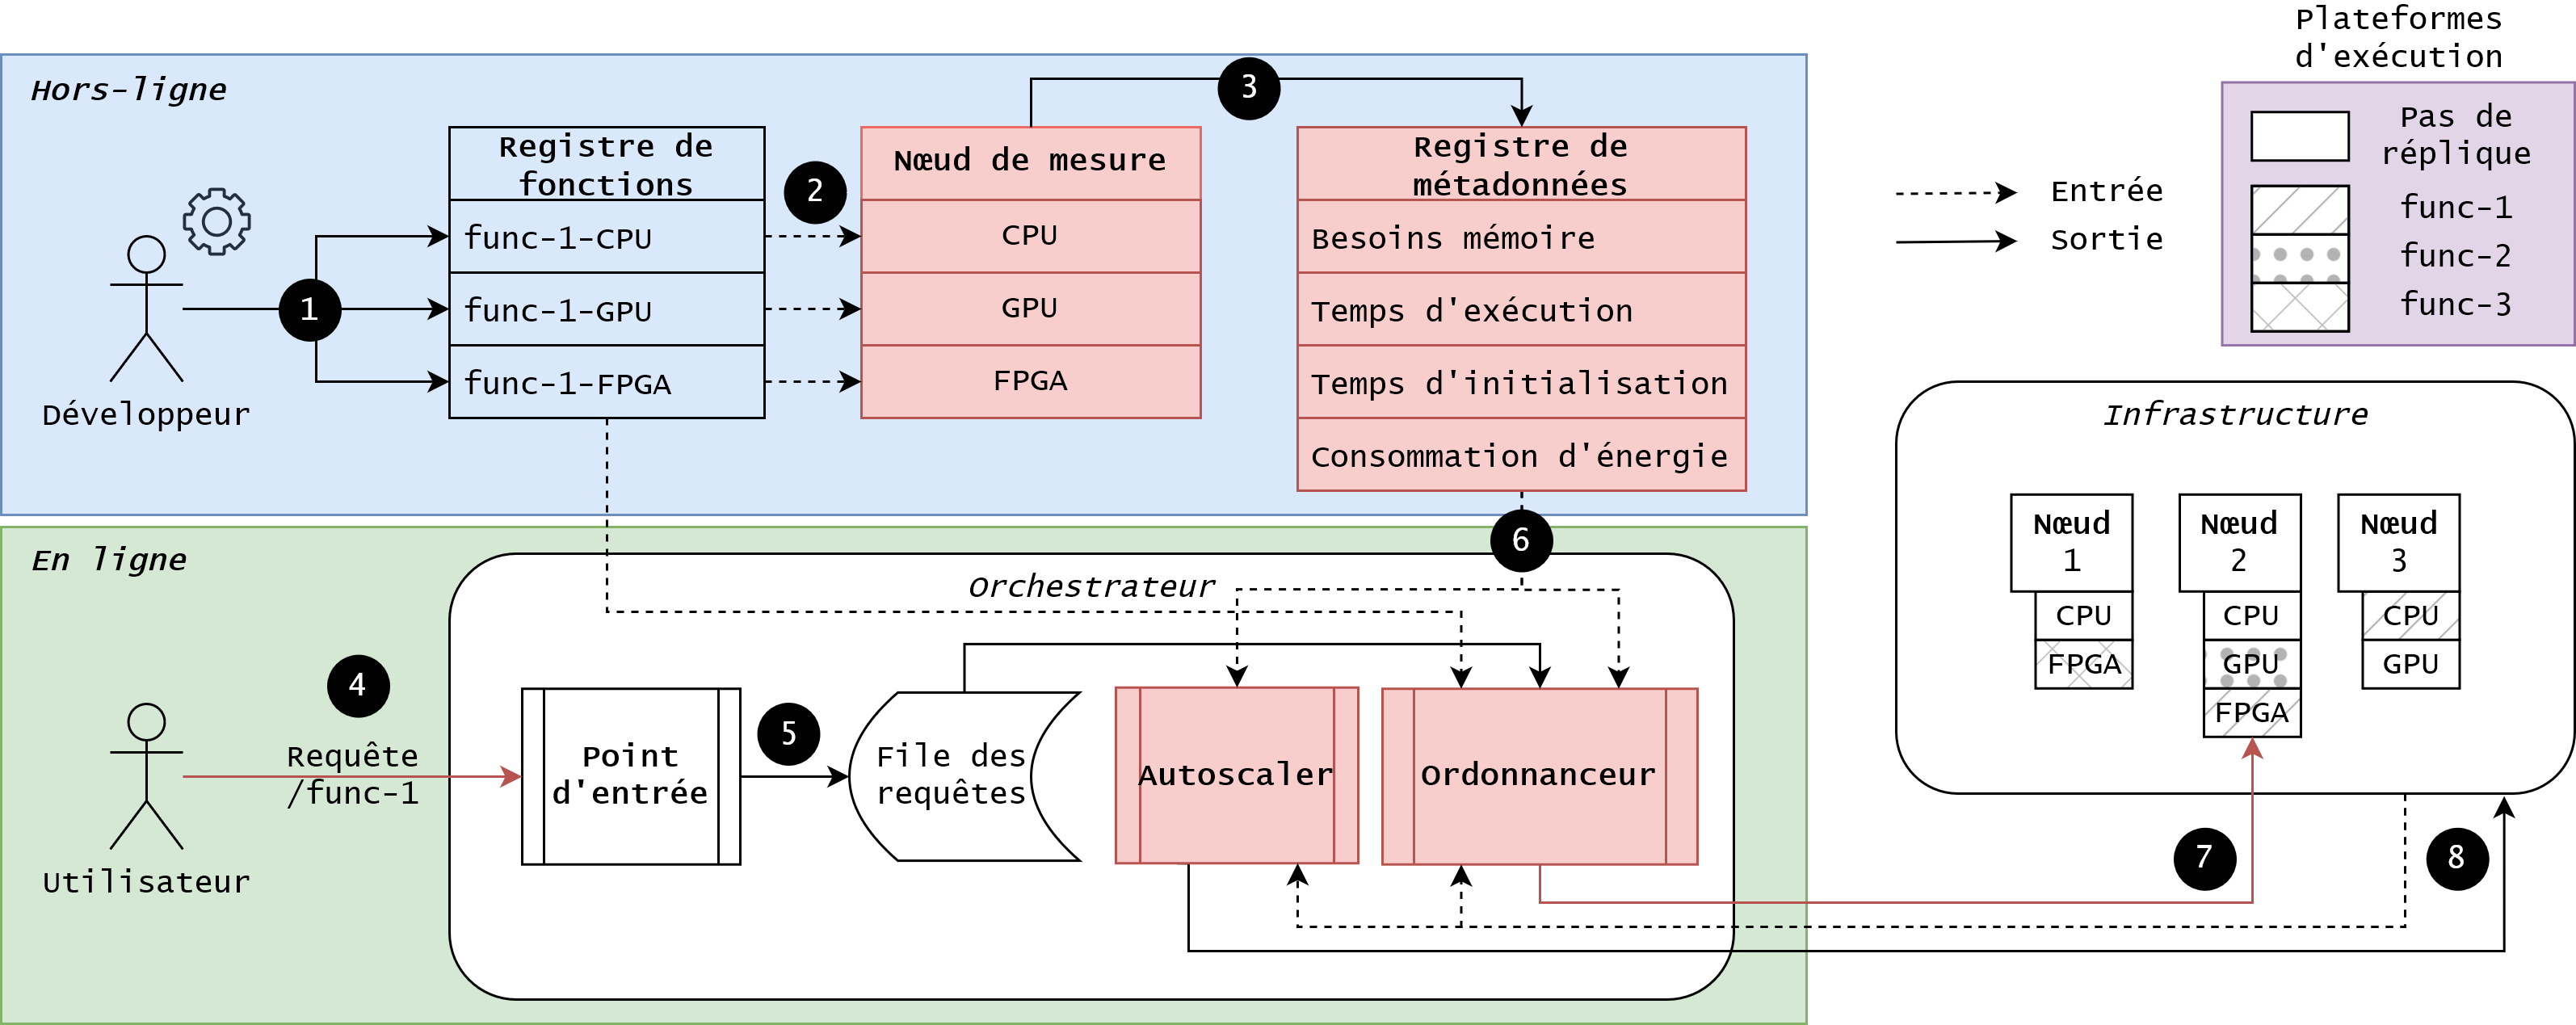
\includegraphics[width=0.9\textwidth]{4_Chapitre4/figures/placement.png}
    \caption{Plateforme serverless pour le déploiement d'une application de détection de deepfake ; vue d'ensemble du système.}
    \label{figure:herofake-placement}
\end{figure*}

La figure~\ref{figure:herofake-placement} illustre le cycle de vie d'une requête entrante dans la plateforme.

\textbf{Phase hors-ligne}. Dans notre plateforme, le cycle de vie de l'application commence par une phase hors-ligne au cours de laquelle le développeur fournit le code de ses fonctions pour différentes architectures matérielles~\Circled{1}. Ce code est stocké dans un registre de fonctions. Les fonctions sont ensuite déployées sur un nœud de mesure~\Circled{2} où elles sont exécutées afin de générer des métadonnées relatives aux fonctions : les besoins en mémoire, le temps d'exécution, le temps de démarrage à froid et la consommation d'énergie pour chaque fonction sont écrits dans un registre de métadonnées~\Circled{3}. La phase hors-ligne doit être exécutée une fois pour une fonction donnée sur une plateforme donnée, elle est décrite dans la section~\ref{section:herofake-offline}.

\textbf{Phase en ligne}. Lorsqu'un utilisateur envoie une requête à l'application~\Circled{4}, il fournit une image d'entrée et spécifie le niveau de qualité de service souhaité. La requête est ajoutée à une file d'attente~\Circled{5} au niveau de l'orchestrateur. Lorsque l'ordonnanceur extrait la requête de la file d'attente, le registre de métadonnées est interrogé pour récupérer les métadonnées de fonction appropriées~\Circled{6}.

L'\textbf{ordonnanceur} tente ensuite de planifier une tâche (c'est-à-dire l'invocation d'une fonction) pour répondre à la requête. Les tâches sont placées sur des \textit{répliques} de fonctions~\Circled{7} déjà déployées. Ces répliques peuvent être des conteneurs ou des machines virtuelles, c'est-à-dire des environnements d'exécution dédiés pour la fonction donnée. Simultanément, l'\textbf{autoscaler} surveille les files d'attente de requêtes dans toutes les répliques de fonctions~\Circled{8}. Le rôle de l'autoscaler est de dimensionner les ressources allouées en fonction des fluctuations de charge pour chaque fonction. L'ordonnanceur et l'autoscaler sont décrits dans la section~\ref{section:herofake-online}.

\section{Phase hors-ligne : mesures et extraction des métadonnées}
\label{section:herofake-offline}

Dans cette section, nous détaillons notre méthodologie et donnons les résultats de la campagne de mesures menée dans le but de caractériser les plateformes d'exécution ainsi que les tâches considérées dans cette contribution.

Ces travaux ont été menés conjointement avec une équipe d'ingénieurs à l'IRT b{\textless\textgreater}com, co-auteurs de la publication associée à ce chapitre~\cite{herofake}.

\subsection{Caractérisation des plateformes d'exécution}

\begin{table}[!ht]
    \caption{Caractérisation des plateformes d'exécution.}
    \begin{center}
    \resizebox{\columnwidth}{!}{%
    \begin{tabular}{|c|c|c|c|c|}
    \hline
                                 \textbf{Plateforme} & \textbf{Type de matériel}& \textbf{Prix (\gls{MSRP}, €)} & \textbf{Énergie au repos (kWh)} \\ \hline
    Intel Xeon ES-1620 v4         & \gls{CPU}           & 294          & 0,067       \\ \hline
    Nvidia GeForce RTX 2070 Super & \gls{GPU}           & 499          & 0,010       \\ \hline
    Xilinx Alveo U250             & \gls{FPGA}          & 7695         & 0,030       \\ \hline
    \end{tabular}%
    }
    \end{center}
    \label{table:herofake-platforms}
\end{table}

La demande grandissante pour l'apprentissage automatique et l'inférence, ainsi que l'augmentation de la consommation d'énergie dans le cloud~\cite{masanetRecalibratingGlobalData2020}, font de l'efficacité énergétique des dispositifs cibles une préoccupation majeure. Les accélérateurs basées sur les \gls{FPGA} sont décrits comme un concurrent pertinent à l'hégémonie des \gls{GPU}. Nous proposons un banc d'essai pour mesurer l'efficacité énergétique de plusieurs plateformes matérielles (\gls{CPU}, \gls{GPU}, \gls{FPGA}) pendant la phase d'inférence pour plusieurs \gls{CNN} utilisés dans le cadre de la détection de deepfake. Notre comparaison porte sur des métriques de consommation d'énergie, de vitesse d'inférence et de précision. Ces mesures sont cruciales pour une orchestration efficace sur des plateformes hétérogènes.

Le \gls{CPU} caractérisé est un Intel Xeon ES-1620 v4 (3,5 GHz) ; le \gls{GPU} est une Nvidia GeForce RTX 2070 Super. Ces deux modèles sont compatibles avec les versions récentes de TensorFlow, une des plateformes principales utilisées pour l'inférence. Si les procédés de fabrication pour ces deux accélérateurs sont comparables, la finesse de gravure à 12 nm pour le \gls{GPU} contre 16 nm pour le \gls{FPGA} pourrait donner un léger avantage au \gls{GPU} dans ce banc d'essai.

En ce qui concerne le \gls{FPGA}, nous avons utilisé l'Alveo U250, une carte dédiée au cloud et fabriquée par Xilinx. Ce \gls{FPGA} est compatible avec Vitis-AI~\footnote{\href{https://github.com/Xilinx/Vitis-AI}{https://github.com/Xilinx/Vitis-AI}}, que nous avons utilisé pour exécuter les tâches d'inférence sur le \gls{FPGA}. Nous avons utilisé la dernière version disponible (v. 2.0) au moment de cette étude. Vitis-AI propose deux méthodes pour l'optimisation des modèles, nécessaire à leur exploitation sur un \gls{FPGA} limité en ressources mémoire. La première est l'élagage, qui consiste à réduire la complexité du modèle par une compression tout en supprimant certaines sections non critiques de l'arbre. La seconde est la quantification, qui consiste à convertir les poids flottants de 32 bits en entiers de 8 bits. Nous avons utilisé cette dernière méthode pour optimiser notre modèle avant la compilation, qui convertit notre modèle en instructions DPU (\textit{Deep Processing Unit}).

La mesure d'énergie au repos rapportée dans le tableau~\ref{table:herofake-platforms} est une moyenne calculée sur cinq minutes de relevés. Nous n'avons pas pris en compte les optimisations automatiques de la tension et de la fréquence du \gls{CPU} (\textit{P-states}~\cite{kwasnickDeterminationCPUUse2011}), ni les optimisations de sa consommation d'énergie au repos (\textit{C-states}~\cite{sueurSlowSleepThat}) mises en œuvre par le fabricant.

\subsection{Caractérisation des tâches logicielles}
\label{section:herofake-offline:workload}

\begin{table}[!ht]
    \caption{Caractérisation des charges de travail.}
    \centering
    \resizebox{\columnwidth}{!}{%
    \begin{tabular}{|c|cc|ccc|ccc|ccc|}
    \hline
    Tâche     & \multicolumn{2}{c|}{Pic mémoire (Go)} & \multicolumn{3}{c|}{Démarrage à froid (s)}                              & \multicolumn{3}{c|}{Temps d'exécution (s)}                         & \multicolumn{3}{c|}{Énergie dynamique (mWh)}                            \\ \hline
             & \multicolumn{1}{c|}{CPU}  & \gls{GPU}  & \multicolumn{1}{c|}{CPU}   & \multicolumn{1}{c|}{GPU}   & \gls{FPGA}   & \multicolumn{1}{c|}{CPU}   & \multicolumn{1}{c|}{GPU}   & \gls{FPGA}  & \multicolumn{1}{c|}{CPU}  & \multicolumn{1}{c|}{GPU}  & \gls{FPGA} \\ \hline
    ResNet50 & \multicolumn{1}{c|}{1,3}  & 3,3  & \multicolumn{1}{c|}{1,232} & \multicolumn{1}{c|}{2,340} & 9,952  & \multicolumn{1}{c|}{0,124} & \multicolumn{1}{c|}{0,024} & 0,009 & \multicolumn{1}{c|}{3,11} & \multicolumn{1}{c|}{1,7}  & 0,5  \\ \hline
    VGG16    & \multicolumn{1}{c|}{1,8}  & 3,3  & \multicolumn{1}{c|}{2,514} & \multicolumn{1}{c|}{4,641} & 14,528 & \multicolumn{1}{c|}{0,143} & \multicolumn{1}{c|}{0,046} & 0,010 & \multicolumn{1}{c|}{4,34} & \multicolumn{1}{c|}{3,43} & 0,55 \\ \hline
    VGG19    & \multicolumn{1}{c|}{1,9}  & 3,4  & \multicolumn{1}{c|}{2,559} & \multicolumn{1}{c|}{4,641} & 14,758 & \multicolumn{1}{c|}{0,167} & \multicolumn{1}{c|}{0,048} & 0,012 & \multicolumn{1}{c|}{5,16} & \multicolumn{1}{c|}{3,58} & 0,65 \\ \hline
    \end{tabular}
    }%
    \label{table:herofake-tasks}
\end{table}

Nous avons caractérisé trois modèles populaires au moment de cette étude. Le premier, ResNet50, est basé sur les réseaux neuronaux résiduels. Il utilise des blocs résiduels et peut être entraîné efficacement~\cite{NEURIPS2019_7716d0fc}. Le second est VGG16 (VGG pour \text{Visual Geometry Group}), qui utilise uniquement des convolutions comme blocs~\cite{DBLP:journals/corr/SimonyanZ14a} et le troisième est VGG19, une variante de VGG16 avec trois couches supplémentaires~\cite{biom10070984}. Ces réseaux sont entraînés sur un \gls{GPU}, l'entraînement n'étant pas le sujet de cette étude.

Les mesures rapportées dans le tableau~\ref{table:herofake-tasks} sont des moyennes calculées sur la base de sur vingt mesures.

\subsection{Mesures de performances}

\begin{figure}[!ht]
    \centering
    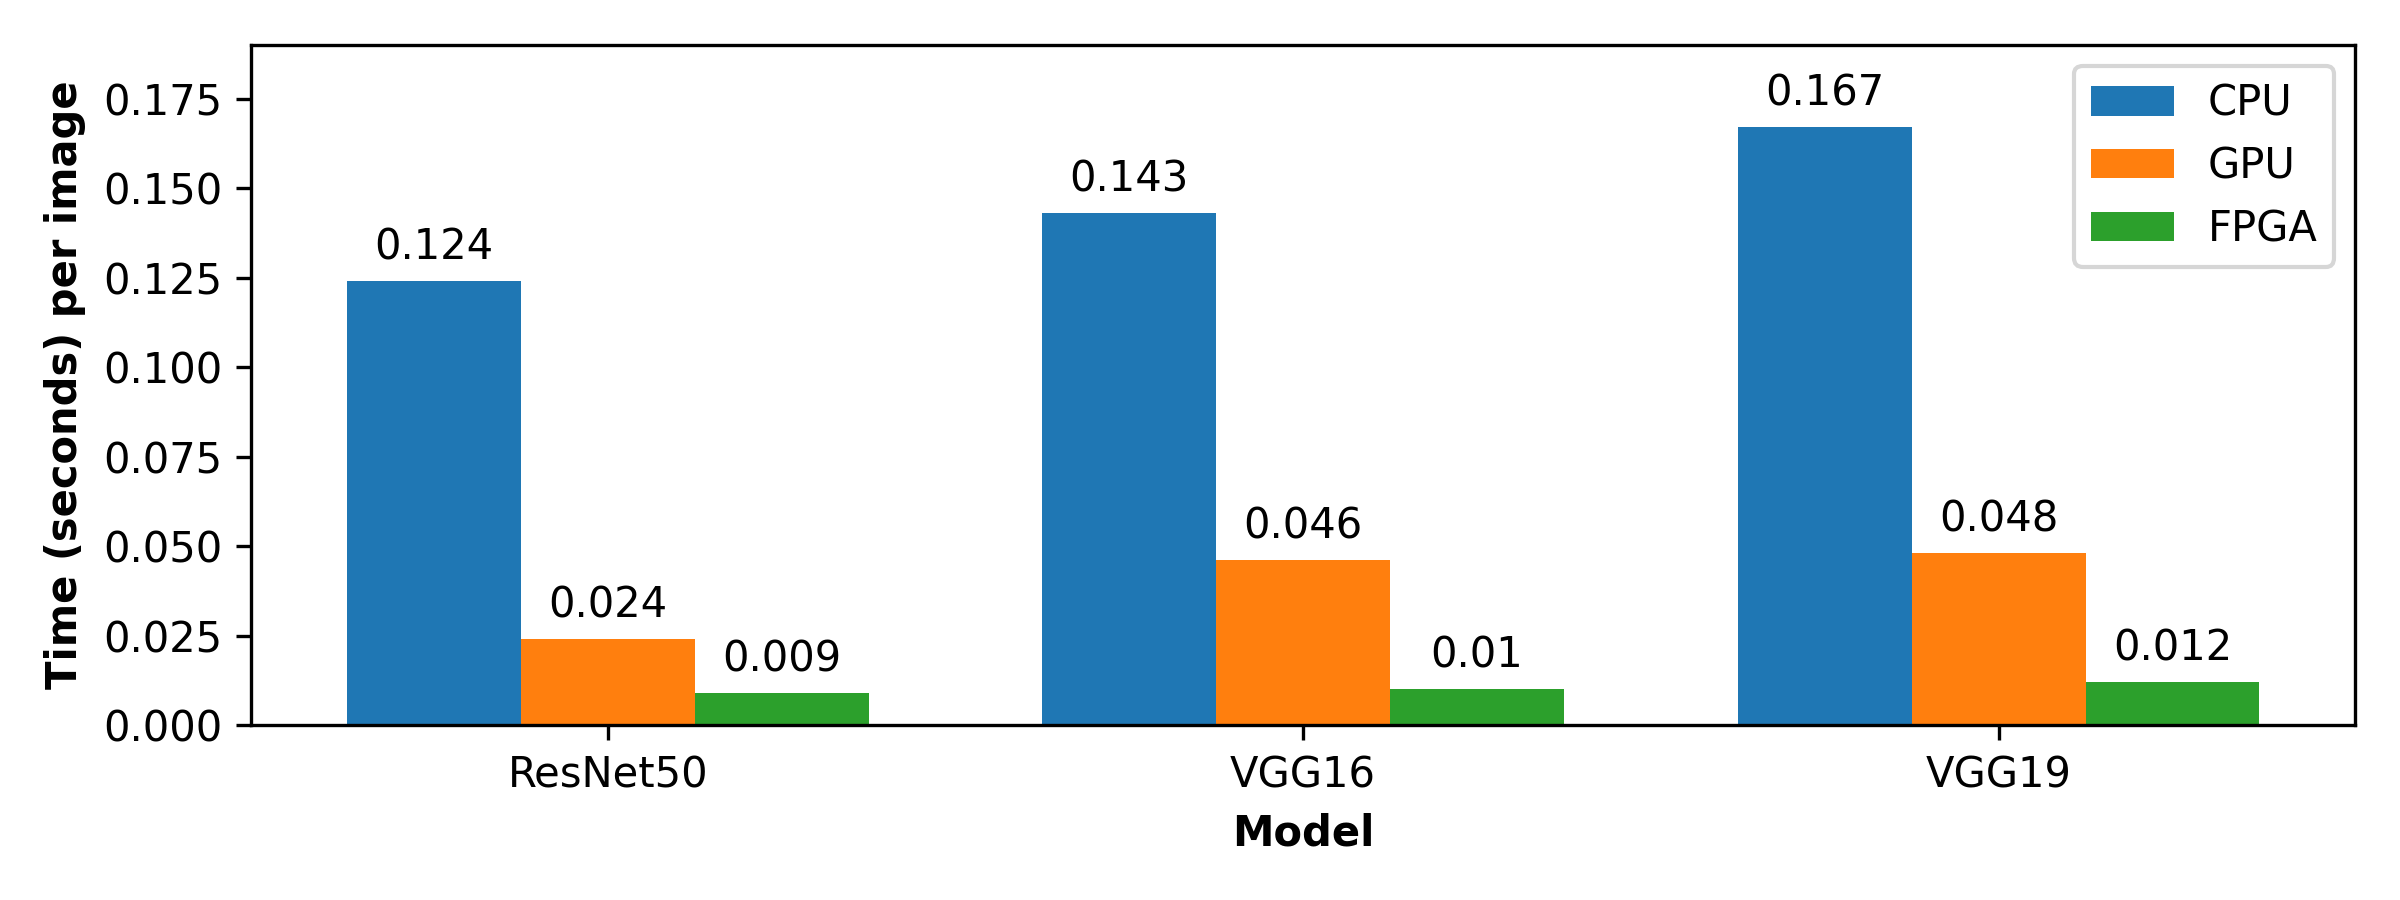
\includegraphics[width=0.7\columnwidth]{4_Chapitre4/figures/characterization/time_of_inference_1_image.png}
    \caption{Temps de l'inférence pour une image avec ResNet50, VGG16 et VGG19.}
    \label{figure:herofake-time-inference}
\end{figure}

La carte d'accélération \gls{FPGA} étant censée être plus efficace qu'un \gls{CPU} ou un \gls{GPU}~\cite{5272532}, la comparaison du temps d'inférence avec ces trois technologies est une première condition pour permettre la comparaison du coût énergétique par image. L'évaluation des performances en termes de temps d'exécution a été réalisée avec les mêmes 10000 images pour les trois modèles différents. Nous avons construit un jeu de données à deux classes : d'une part, de vraies images provenant du jeu de données CelebA~\cite{https://doi.org/10.48550/arxiv.1411.7766}, et d'autres part des images synthétiques générées à l'aide d'un \textit{Generative Adversarial Network} (GAN)~\cite{jimaging7080128}. La quantification et la compilation du modèle ont été effectuées avec Vitis-AI afin de l'exécuter sur le \gls{FPGA}. En ne considérant que le temps d'inférence, il s'est avéré que sur les trois modèles testés (ResNet50, VGG16 et VGG19), le \gls{FPGA} est de 13,08 à 13,79 fois plus rapide que le \gls{CPU} mais aussi de 2,52 à 4,48 fois plus rapide que le \gls{GPU} (voir figure~\ref{figure:herofake-time-inference}).

\subsection{Mesures de consommation d'énergie}

\begin{figure}[!ht]
    \centering
    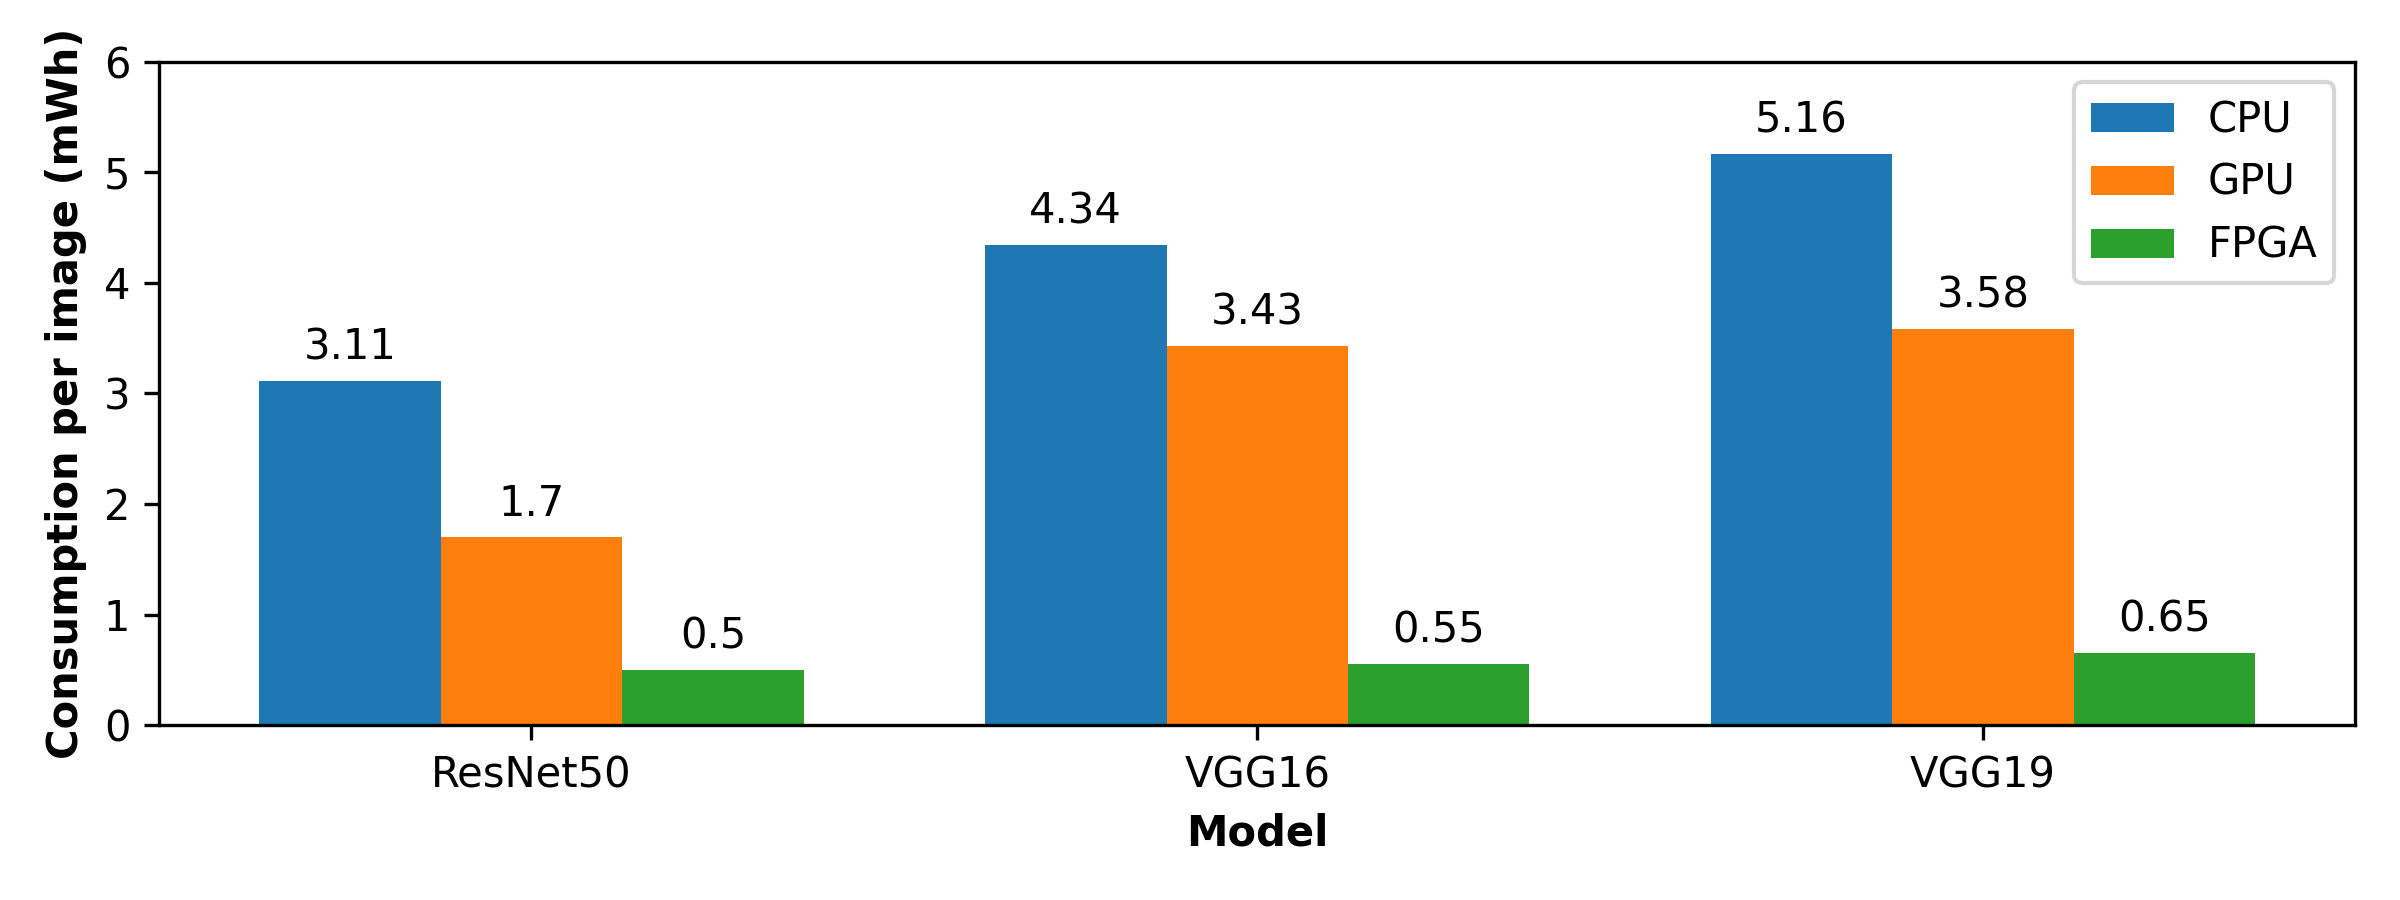
\includegraphics[width=0.7\columnwidth]{4_Chapitre4/figures/characterization/consumption_per_image.png}
    \caption{Consommation d'énergie pour l'inférence, par image (mWh).}
    \label{figure:herofake-consumption-per-image}
\end{figure}

La consommation d'énergie instantanée mesurée pendant l'inférence correspond à la consommation globale de la machine (y compris le \gls{CPU}, la mémoire, la carte mère et l'alimentation) pendant l'exécution de l'inférence.
Les mesures ont été effectuées à l'aide d'une alimentation spécifique (\gls{PDU}, pour \textit{Power Distribution Unit}), en l'occurrence une Raritan PX3-5190R, capable de surveiller la puissance instantanée et la consommation d'énergie du serveur (Dell Precision T5810). Les résultats montrent que l'inférence sur le \gls{CPU} produit la consommation d'énergie instantanée la plus faible. Ce résultat est assez attendu car l'inférence sur \gls{GPU} ou \gls{FPGA} induit également une consommation d'énergie par le \gls{CPU}.

Cependant, la seule consommation d'énergie instantanée ne reflète pas correctement le coût total de chaque plateforme. Le temps d'exécution nécessaire pour traiter toutes les images doit être pris en compte. La mesure pertinente est le coût énergétique par image. La consommation d'énergie a été mesurée en kilowattheures (kWh) pour les 10000 images, puis convertie en milliwattheures (mWh) par image. De ce point de vue, il est clair que le \gls{FPGA} est le plus économe en énergie étant donné le temps d'exécution : sa consommation est de 6,2 à 6,9 fois moindre que pour le \gls{CPU}, et de 3,3 à 6,2 fois moindre que pour le \gls{GPU} (voir figure~\ref{figure:herofake-consumption-per-image}).

\subsection{Discussion}

\begin{figure}[!ht]
    \centering
    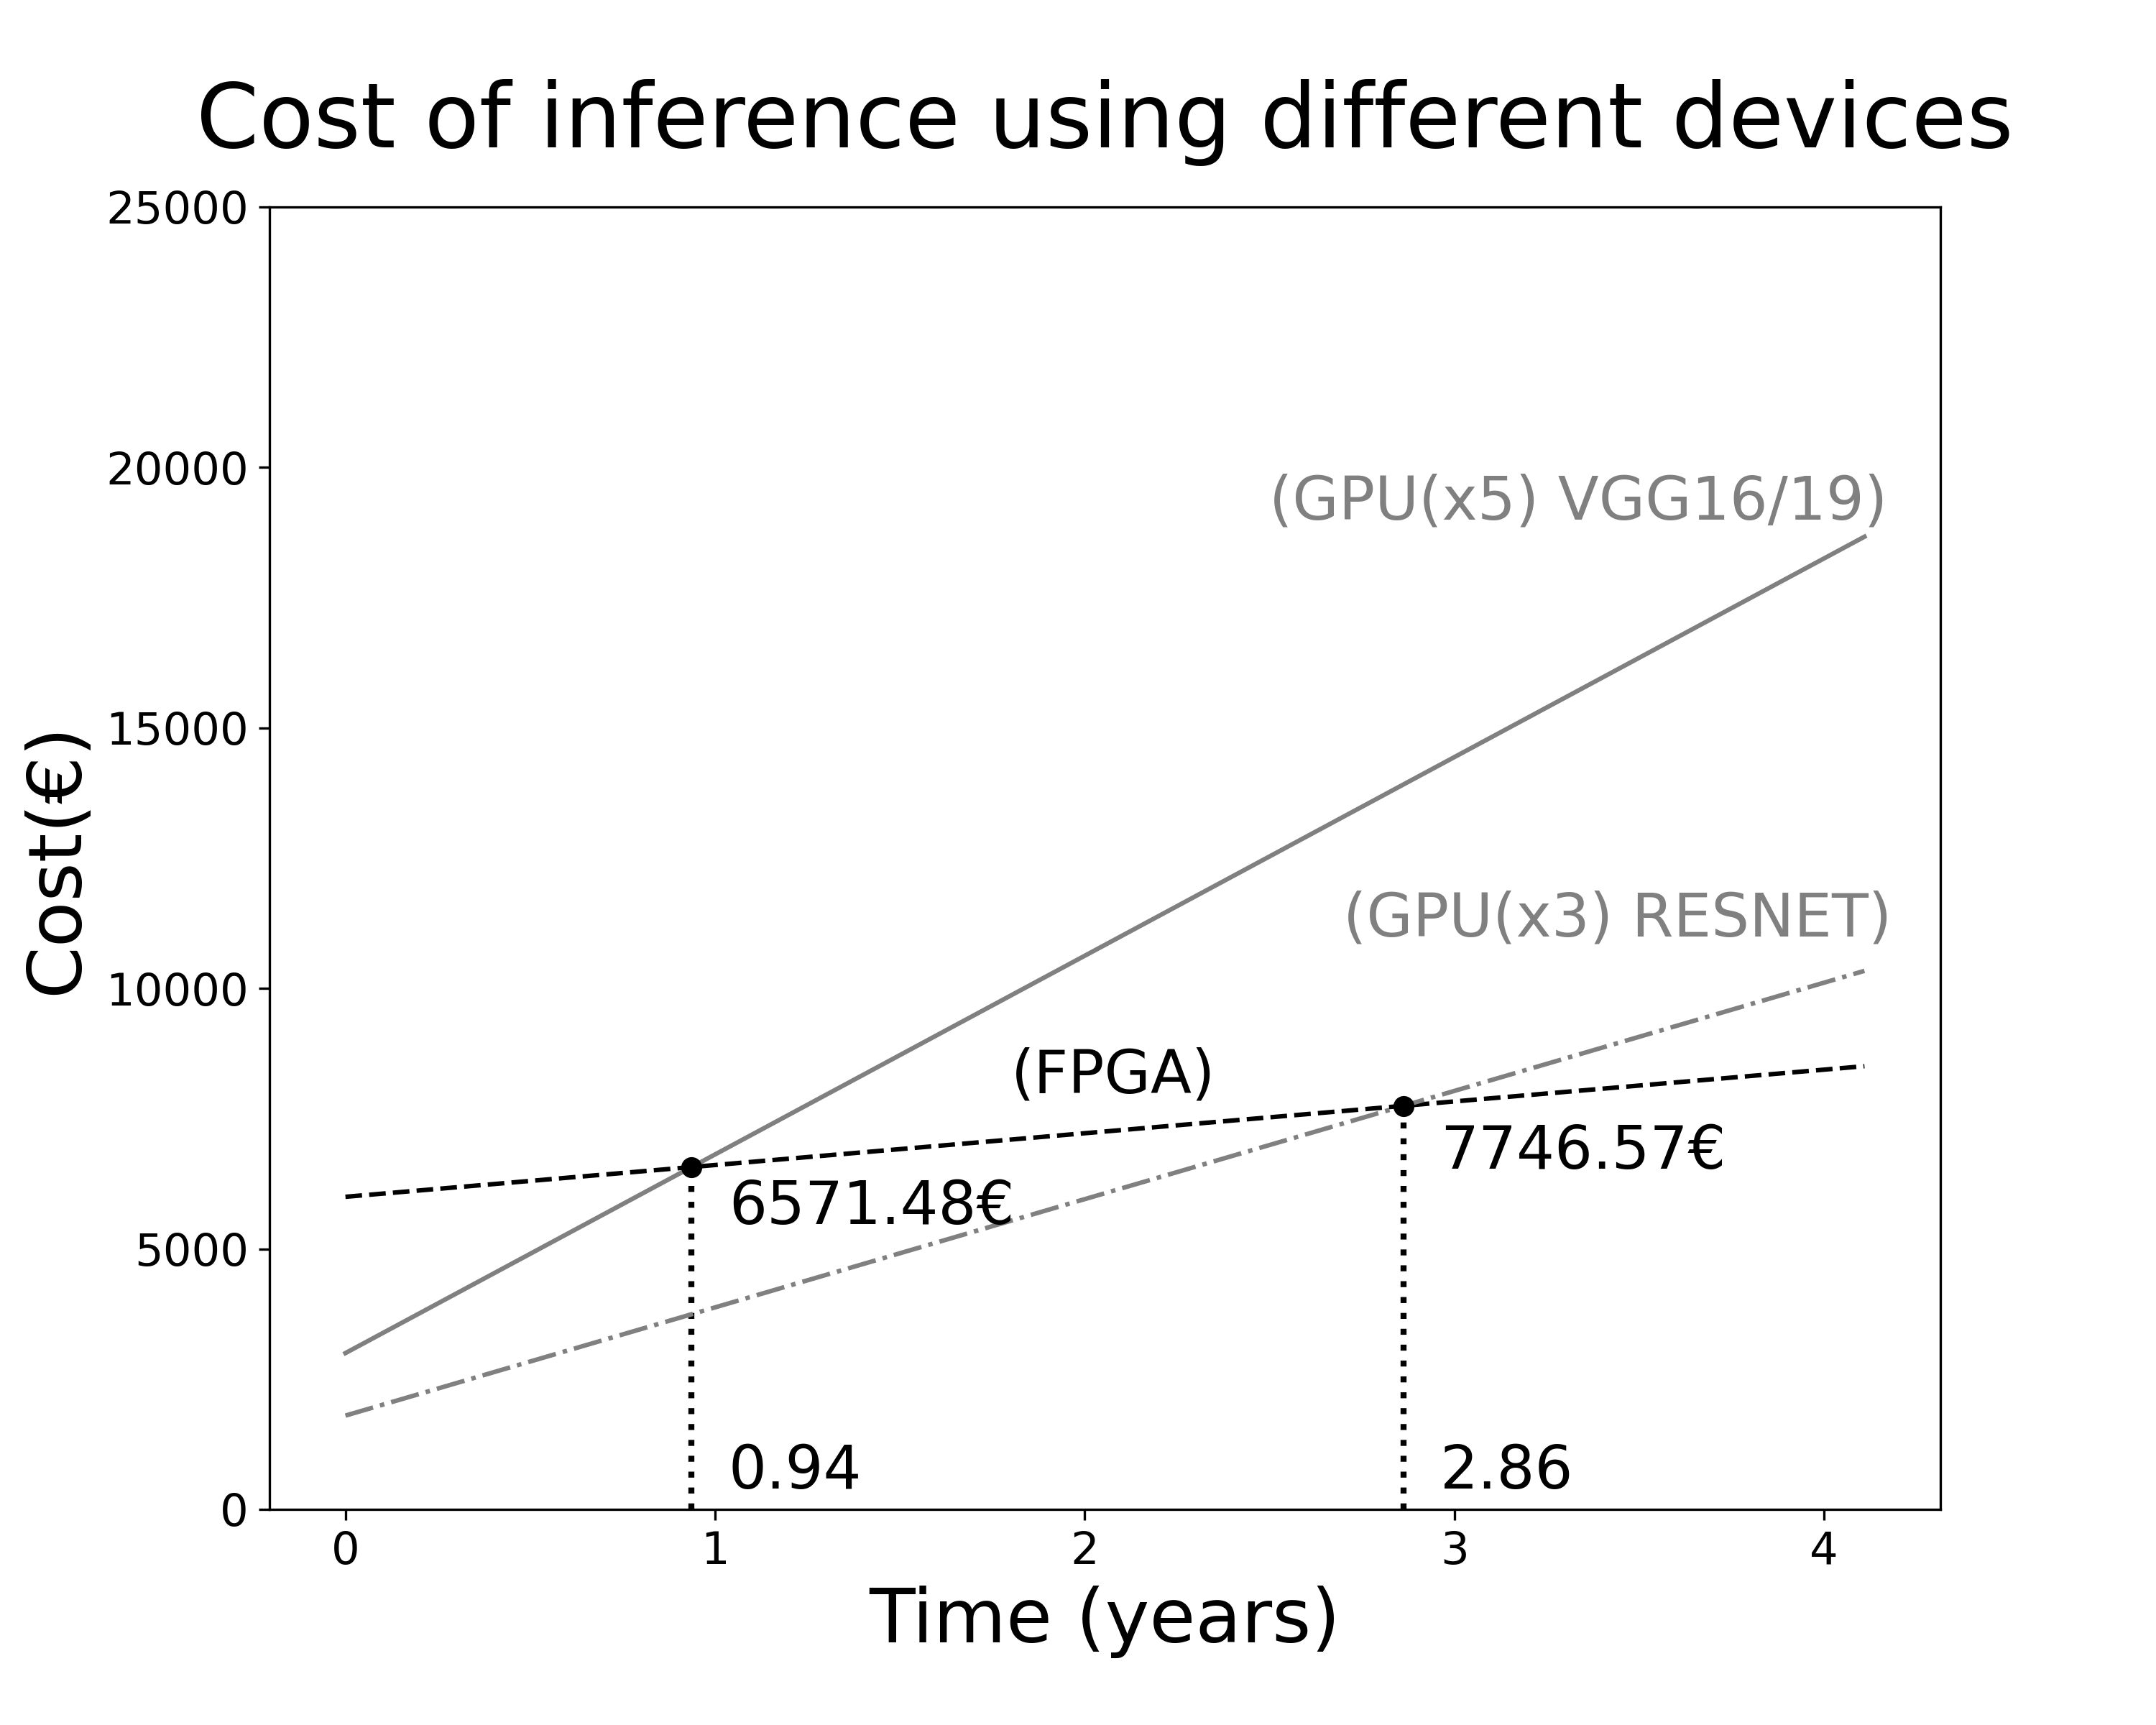
\includegraphics[width=0.6\textwidth]{4_Chapitre4/figures/characterization/cost_devices_time.png}
    \caption{Coût total de l'inférence dans le temps pour les plateformes considérées.}
    \label{figure:herofake-cost-over-time}
\end{figure}

Les résultats de ce banc d'essai montrent un net avantage en faveur du \gls{FPGA} pour l'inférence en termes de performance et d'efficacité énergétique. Les gains de performance sont significatifs, en particulier avec les réseaux d'apprentissage profond plus complexes~\cite{8782524}.

Cependant, la consommation d'énergie brute du dispositif ne reflète pas le coût total de la solution. En effet, il faut également inclure le coût de l'équipement lui-même. C'est un point important dans la comparaison entre \gls{GPU} et \gls{FPGA}, car il existe un écart de prix important entre les deux technologies : le \gls{GPU} (RTX 2070 Super) utilisé pour ce banc d'essai a été lancé aux alentours de 600€, alors que le \gls{FPGA} (Alveo U250) est vendu aux alentours de 6000€. En Europe, le coût de l'électricité pour effectuer l'inférence est très faible (nous avons utilisé la moyenne européenne de 0,1833€ par kWh au moment de cette étude~\cite{energy-price}), comparé au coût initial du dispositif : la durée d'exécution nécessaire pour bénéficier de l'avantage-coût du \gls{FPGA} est de l'ordre de plusieurs mois de fonctionnement continu. La figure~\ref{figure:herofake-cost-over-time} représente le coût cumulé (en euros) de l'utilisation d'un serveur avec accélération \gls{GPU} ou \gls{FPGA} en fonction du temps (en années). Notre estimation du coût comprend le nombre de \gls{GPU} nécessaires et leur coût pour rivaliser avec les performances des \gls{FPGA}, et est pondérée d'un facteur 2x~\cite{shehabiUnitedStatesData2016} pour tenir compte de la consommation d'énergie totale de l'infrastructure (principalement le refroidissement et les équipements réseau). Le \gls{FPGA} peut devenir une solution rentable après quelques mois pour les \gls{CNN} complexes. Pour les réseaux moins complexes, l'avantage financier du \gls{FPGA} est atteint après plus de deux ans.

\begin{figure}[!ht]
    \centering
    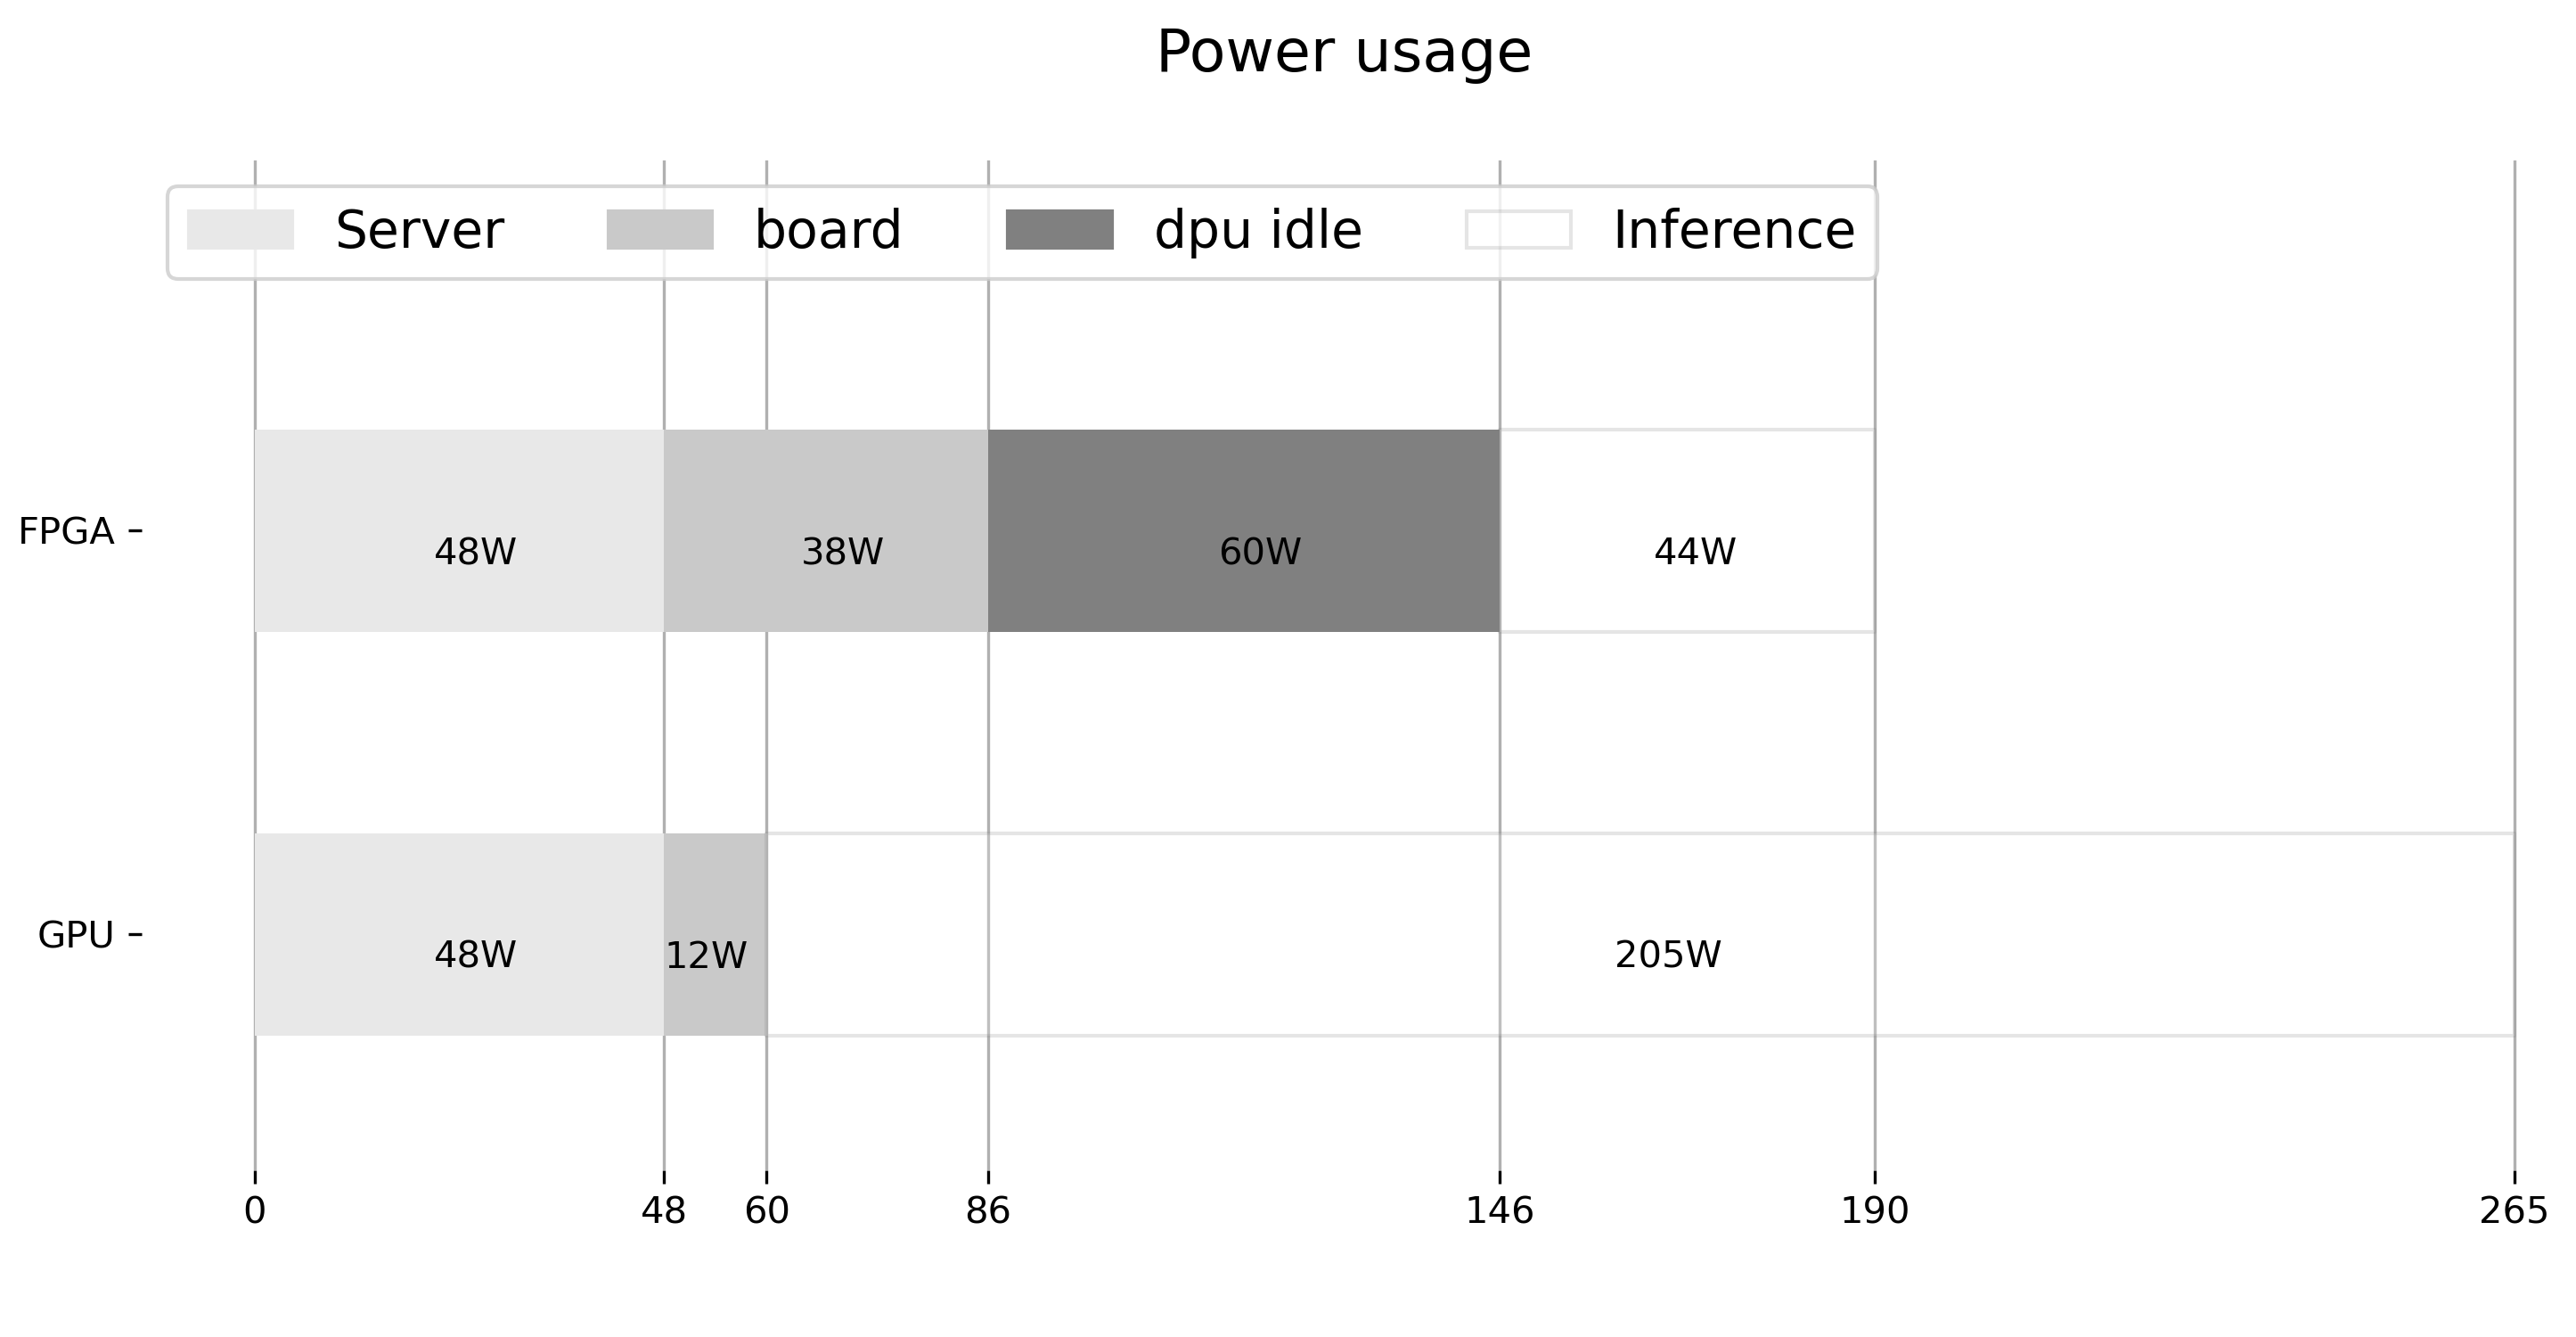
\includegraphics[width=\columnwidth]{4_Chapitre4/figures/characterization/power_usage.png}
    \caption{Détail de l'énergie consommée par le \gls{FPGA} et le \gls{GPU}.}
    \label{figure:herofake-power-usage}
\end{figure}

L'analyse précédente est valable dans le cas où l'inférence est toujours effectuée à pleine charge. En effet, lorsque l'on décompose la consommation d'énergie du \gls{GPU} entre sa consommation au repos et sa consommation lors de l'inférence, il est clair que le \gls{GPU} est capable d'adapter dynamiquement sa consommation d'énergie en fonction de l'intensité du traitement. Le \gls{FPGA}, quant à lui, semble avoir une gestion de l'énergie très limitée. Une fois le modèle (\textit{DPU}, pour \textit{Deep Learning Processor Unit}) chargé dans le \gls{FPGA}, la consommation d'énergie au repos est mesurée à un niveau élevé (figure~\ref{figure:herofake-power-usage}). Toutefois, ce n'est pas le cas pour tous les \gls{FPGA} : certains modèles proposent une gestion plus fine de la consommation d'énergie, avec un mode au repos et un mode suspendu qui permettent un réveil plus ou moins rapide, à des niveaux de consommation plus faibles~\cite{shahzadInvestigatingEnergyConsumption}.
En plus des 38W consommés au repos par la carte \gls{FPGA}, on observe une consommation résiduelle de 60W, même lorsque le dispositif est inactif. Si des évolutions en matière d'implantation du DPU sur le \gls{FPGA} peuvent limiter l'impact de ce problème (par exemple en réduisant la fréquence d'horloge lorsqu'il est inactif), son influence sur le coût total doit être pris en compte si le dispositif n'est pas toujours utilisé à pleine charge. Avec seulement 12W d'énergie au repos, le \gls{GPU} est un meilleur candidat lorsque l'utilisation à pleine charge du dispositif n'est pas garantie.

Comme la tendance vers des \gls{CNN} plus complexes se poursuit~\cite{8807741}, l'utilisation de dispositifs les plus efficaces possibles devient un défi majeur. La solution \gls{FPGA} offre une nouvelle option pour effectuer l'inférence. Cependant, les \gls{FPGA} ne remplacent pas encore les \gls{GPU} : le flot de compilation reste complexe et coûteux en temps. Il est nécessaire de trouver un compromis entre la flexibilité des \gls{GPU} et l'efficacité des \gls{FPGA}. La section suivante traite d'un premier orchestrateur qui prend en compte la caractérisation mentionnée ci-dessus pour l'allocation et l'ordonnancement de ressources hétérogènes.

\section{Phase en ligne : allocation des ressources et placement des tâches}
\label{section:herofake-online}

Dans cette section, nous formulons le problème que notre contribution cible, puis nous donnons une description détaillée de notre modèle. Enfin, nous présentons une description formelle de notre stratégie pour la mise à l'échelle automatique des ressources et l'ordonnancement des tâches.

\subsection{Défis pour l'orchestration dynamique}

L'ordonnancement des charges de travail dans le paradigme serverless est un problème à deux volets : les fournisseurs doivent gérer dynamiquement l'allocation des ressources (c'est-à-dire dimensionner les ressources matérielles allouées lors de la mise à l'échelle du nombre de répliques pour une fonction) et le placement des tâches (c'est-à-dire l'ordonnancement des requêtes utilisateur sur les répliques existantes).

L'augmentation du nombre de répliques pose un problème de performances : lorsqu'une nouvelle réplique est créée, que ce soit sous la forme d'un conteneur ou d'une machine virtuelle, l'environnement d'exécution doit passer par sa phase d'initialisation. C'est ce que l'on appelle un "démarrage à froid".

Les solutions commerciales telles que \gls{AWS} Lambda évitent souvent le problème du démarrage à froid en maintenant des réserves d'environnements d'exécution "chauds"~\cite{vahidiniaColdStartServerless2020}, c'est-à-dire déjà initialisés, et en attente de nouvelles requêtes. Ces environnements peuvent aussi être démarrés par anticipation et mis en pause dans un état post-initialisation. Lorsque l'activité reprend, les requêtes entrantes peuvent être servies sans souffrir d'un délai de démarrage à froid, au détriment du multiplexage des ressources du côté du fournisseur. Bien que cette solution permette de réduire, voire d'éliminer les délais de démarrage à froid, elle pèse sur la capacité du fournisseur à maximiser l'utilisation des ressources, et augmente le coût total de possession (\gls{TCO}, pour \textit{Total Cost of Ownership}).

En outre, les applications de \textit{Machine Learning as a Service} (\gls{MLaaS}) présentent des motifs d'utilisation très fluctuants~\cite{gujaratiSwayamDistributedAutoscaling2017}, ce qui renforce l'argument selon lequel une stratégie d'allocation réactive des ressources est nécessaire pour dimensionner efficacement l'infrastructure. Cependant, comme le temps d'exécution des tâches d'inférence est de l'ordre du centième ou du dixième de seconde, tandis que le temps d'initialisation des environnements d'exécution est plutôt de l'ordre de quelques secondes~\cite{mancoMyVMLighter2017}, nous avons besoin d'un mécanisme pour éviter de souffrir d'énormes coûts en latence pour l'exécution des fonctions.

Les tâches critiques nécessitent des garanties de niveau de service de la part du fournisseur. Les accords de niveau de service dans le cloud consistent généralement à convenir d'un taux de disponibilité des ressources dans le temps ; si le fournisseur ne respecte pas cet accord, une remise est proposée au client. Bien que cela puisse fonctionner pour des ressources réservées, nous pouvons voir que cela n'a pas de sens dans le paradigme serverless. La possibilité de garantir le temps de réponse des fonctions permettrait à un fournisseur serverless de proposer des accords de niveau de service par requête~\cite{zhangMArkExploitingCloud}.

L'utilisation d'accélérateurs matériels est une possibilité pour améliorer les rapports performance-coût. Bien qu'il s'agisse d'un investissement important (voir figure~\ref{figure:herofake-cost-over-time}), ces dispositifs permettent d'accélérer considérablement les tâches parallèles (voir figure~\ref{figure:herofake-time-inference}), améliorant ainsi le temps de réponse des fonctions, avec un coût énergétique réduit (voir figure~\ref{figure:herofake-consumption-per-image}).

\subsection{Modèle de tâche} \label{model:tasks}

\begin{table}[!ht]
    \caption{Dictionnaire des notations.}
    \begin{center}
    \scalebox{0.85}{
        \begin{tabularx}{\linewidth}{|c|Z|}
            \hline \textbf{Notation} & \textbf{Description} \\ \hline
            $f_{N, P}$ & Une fonction $f$ déployée pour exécution sur une plateforme $P$ disponible sur un nœud $N$ \\ \hline
            $QP$ & Pénalité sur qualité de service \\ \hline
            $QD$ & Facteur de ralentissement autorisé par niveau de qualité de service \\ \hline
            $WCET$ & Pire temps d'exécution \\ \hline
            $TT$ & Temps total pour une tâche \\ \hline
            $WT$ & Temps d'attente \\ \hline
            $CST$ & Temps de démarrage à froid \\ \hline
            $ET$ & Temps d'exécution nominal d'une fonction \\ \hline
            $EC$ & Consommation d'énergie \\ \hline
            $HP$ & Prix du matériel \\ \hline
            $TC$ & Consolidation des tâches \\ \hline
            $Q$ & File d'attente des requêtes dans une réplique \\ \hline
            $replicaCount_{f}$ & Nombre de répliques dans le système pour une fonction $f$ \\ \hline
            $concurrency_{f}$ & Nombre moyen de requêtes en attente pour une fonction $f$ \\ \hline
            $threshold$ & Seuil de concurrence pour les répliques d'une fonction sous Knative \\ \hline
            $replicaCount_{f, h}$ & Nombre de répliques dans le système pour une fonction $f$ sur un type de matériel $h$ \\ \hline
            $concurrency_{f, h}$ & Nombre moyen de requêtes en attente pour une fonction $f$ sur un type de matériel $h$ \\ \hline
            $x_{f, h}$ & Seuil de concurrence pour les répliques d'une fonction $f$ sur un type de matériel $h$ \\ \hline
            $scaleCost_{{f}_{N, P}}$ & Coût de la création d'une nouvelle réplique pour une fonction $f$ sur une plateforme $P$ disponible sur un nœud $N$ \\ \hline
            $schedCost_{{f}_{N, P}}$ & Coût de l'ordonnancement d'une tâche pour une fonction $f$ sur une plateforme $P$ disponible sur un nœud $N$ \\ \hline
        \end{tabularx}
    }
    \label{table:herofake-notation}
    \end{center}
\end{table}

Les applications sont composées de fonctions. L'exécution d'une fonction pour répondre à une requête utilisateur est appelée \textit{tâche}. Dans notre contribution, il n'y a pas de dépendances entre ces tâches : l'application est composée de fonctions pures et sans état. Les évènements qui déclenchent l'exécution d'une tâche arrivent dans le système à un intervalle aléatoire et borné. Nous formulons l'hypothèse qu'une requête aboutit toujours et conduit à l'exécution d'une \textit{tâche} (une instanciation d'une \textit{fonction}). Lorsqu'une tâche a commencé son exécution sur la plateforme qui lui a été attribuée, elle s'exécute pendant la totalité de son temps d'exécution. Nous ne prenons pas en compte la préemption ou les défaillances dans cette contribution : une tâche termine toujours son exécution avec succès, même si son temps de réponse peut dépasser son \textit{échéance}, c'est-à-dire son temps de réponse total attendu étant donné le niveau de qualité de service qui lui est associé. Nous ne tenons pas compte des interférences possibles entre les charges de travail sur le même nœud~\cite{dartoisInvestigatingMachineLearning2021}. 

Nous considérons des tâches qui peuvent être exécutées sans distinction sur des plateformes d'exécution hétérogènes. Dans le contexte de notre étude de cas, la mise en œuvre des différentes fonctions a été réalisée au cas par cas pour chaque plateforme ; cependant, des travaux existent qui permettent une compilation croisée automatique pour des architectures hétérogènes~\cite{hortaXartrekRuntimeExecution2021, 10.1145/3445814.3446699}. Les métadonnées suivantes ont été mesurées pour chaque fonction, sur chaque plateforme d'exécution :

\begin{itemize}
    \item \textit{Besoins mémoire en pic} -- la quantité maximum de mémoire allouée par le système d'exploitation et mesurée pendant l'exécution de la fonction (en Go) ;
    \item \textit{Durée de démarrage à froid} -- la durée de l'initialisation de l'environnement lors de l'exécution de la tâche sur une plateforme qui n'a pas la fonction en cache en mémoire principale ;
    \item \textit{Temps d'exécution} -- la durée prévue pour l'exécution effective de la tâche durant la phase de calcul (on n'y inclut pas la phase d'initialisation) ;
    \item \textit{Consommation d'énergie} -- la différence entre l'énergie statique (au repos) et l'énergie dynamique (en charge) consommée par la plateforme d'exécution lorsqu'elle exécute la tâche.
\end{itemize}

L'équation~\ref{eq:herofake-HRO-total-time} décompose le temps de réponse attendu pour l'exécution d'une fonction $f$ sur une plateforme $P$ sur un nœud $N$.

\begin{equation}
    {TT}_{{f}_{N, P}} = {WT}_{{f}_{N, P}} + {CST}_{{f}_{N, P}} + {ET}_{{f}_{N, P}}
\label{eq:herofake-HRO-total-time}
\end{equation}

Où :

\begin{itemize}
    \item ${WT}_{{f}_{N, P}}$ correspond à la durée de la décision d'ordonnancement, y compris le temps passé par la requête en file d'attente ;
    \item ${CST}_{{f}_{N, P}}$ est la durée d'initialisation de la fonction, y compris son temps potentiel de démarrage à froid ;
    \item ${ET}_{{f}_{N, P}}$ est le temps d'exécution de la fonction sur la plateforme.
\end{itemize}

Nous proposons différents niveaux de qualité de service en fonction des besoins des utilisateurs en matière de garanties sur le temps de réponse. Chaque niveau de qualité de service présente un \textit{facteur de ralentissement} différent (noté $QD$ dans l'équation~\ref{eq:herofake-task-penalty}) -- un facteur par lequel le pire temps d'exécution d'une fonction est multiplié pour donner une limite haute au temps de réponse de cette fonction pour ce niveau de qualité de service.

Le temps d'exécution prédit pour une fonction est toujours basé sur le pire temps d'exécution (noté $WCET_{f}$), c'est-à-dire le temps d'exécution d'une tâche lorsqu'elle est programmée sur la plateforme d'exécution présentant le niveau de performances le plus faible pour cette fonction :

\begin{equation}
    \forall \, (N, P), \, WCET_{f} = \max ET_{N, P}
\label{eq:herofake-task-wcet}
\end{equation}

Une fois qu'une tâche est programmée sur une plateforme d'exécution, elle passe par sa durée totale d'exécution décrite dans l'équation~\ref{eq:herofake-HRO-total-time}. L'échéance de la tâche est calculée en multipliant le pire temps de réponse de la fonction (tel qu'exprimé dans l'équation~\ref{eq:herofake-task-wcet}) par le facteur de ralentissement associé au niveau de qualité de service de la requête de l'utilisateur. L'équation~\ref{eq:herofake-task-penalty} montre que nous fixons une valeur booléenne $QP_{f_{N, P}}$ pour chaque invocation de fonction si la tâche dépasse son échéance : on dit alors que la tâche est en \textit{pénalité}.

\begin{equation}
    QP_{f_{N, P}} =
    \begin{cases}
    1 & \text{if} \quad TT_{f_{N, P}} \cdot QD_{f_{N, P}} > WCET_{f} \\
    0 & \text{if} \quad TT_{f_{N, P}} \cdot QD_{f_{N, P}} \leq WCET_{f}
    \end{cases}
\label{eq:herofake-task-penalty}
\end{equation}

\subsection{Stratégie d'allocation de ressources} \label{section:herofake-autoscaling-strategy}

Dans une plateforme serverless, l'\textit{autoscaler} a la responsabilité d'allouer des ressources matérielles pour les exécutions de fonctions. Pour toute fonction, un autoscaler peut allouer $n$ \textit{répliques}. Le nombre de répliques pour une fonction donnée à un moment donné détermine son niveau de concurrence.

Dans Knative, le nombre de répliques pour une fonction donnée (équation~\ref{eq:herofake-kn-replica-count}) dépend de la charge moyenne glissante pour une fonction, c'est-à-dire le nombre moyen de requêtes en attente pour la fonction sur une fenêtre de 60 secondes (concurrence dans le système par fonction). Il est borné par un seuil de concurrence par réplique, c'est-à-dire le nombre maximum de requêtes en file d'attente dans la réplique à tout moment. La valeur par défaut dans Knative est de 100 requêtes en attente dans chaque réplique~\footnote{\href{https://knative.dev/docs/serving/autoscaling/}{https://knative.dev/docs/serving/autoscaling/}}.

\begin{equation}
    replicaCount_{f} = \frac{concurrency_{f}}{threshold}
\label{eq:herofake-kn-replica-count}
\end{equation}

Ce mécanisme de dimensionnement permet d'allouer des \gls{CPU} sous Knative, en réaction aux changements du niveau concurrence dans le système. La principale contribution que nous proposons pour l'autoscaler de notre plateforme serverless est d'améliorer Knative afin de prendre en compte l'hétérogénéité des plateformes d'exécution.

Le mécanisme simple de Knative ne fonctionne pas lorsque l'infrastructure est constituée d'une variété de plateformes d'exécution. En effet, ces plateformes présentent différents niveaux de performance, de consommation d'énergie et de coût. Cela a une conséquence sur le nombre de répliques que le fournisseur doit déployer sur ces plateformes : pour un niveau de charge donné, des répliques hétérogènes seront capables de traiter un nombre différent de tâches dans le même délai. Pour que notre plateforme puisse gérer l'hétérogénéité de l'infrastructure sous-jacente, nous proposons d'associer le niveau de charge à un nombre de répliques \textbf{par fonction} et \textbf{par type de matériel}, comme montré dans l'équation~\ref{eq:herofake-HRO-replica-count}.

La figure~\ref{figure:herofake-orchestration-scaling} illustre ce mécanisme de dimensionnement. Le nombre de répliques pour une fonction donnée, pour un type de matériel donné (équation~\ref{eq:herofake-HRO-replica-count}) dépend du \textbf{niveau de concurrence moyen} par plateforme matérielle observé dans le système (\textit{i.e.} la moyenne du nombre de requêtes en file d'attente pour une fonction, pour un type de matériel), rapporté au \textbf{seuil de concurrence} déterminé par type de matériel (équation~\ref{eq:herofake-HRO-concurrency-target}, \textit{i.e.} la taille de la file d'attente dans la réplique ; correspond à la zone mauve hachurée dans la figure).

\begin{figure}[!ht]
    \centering
    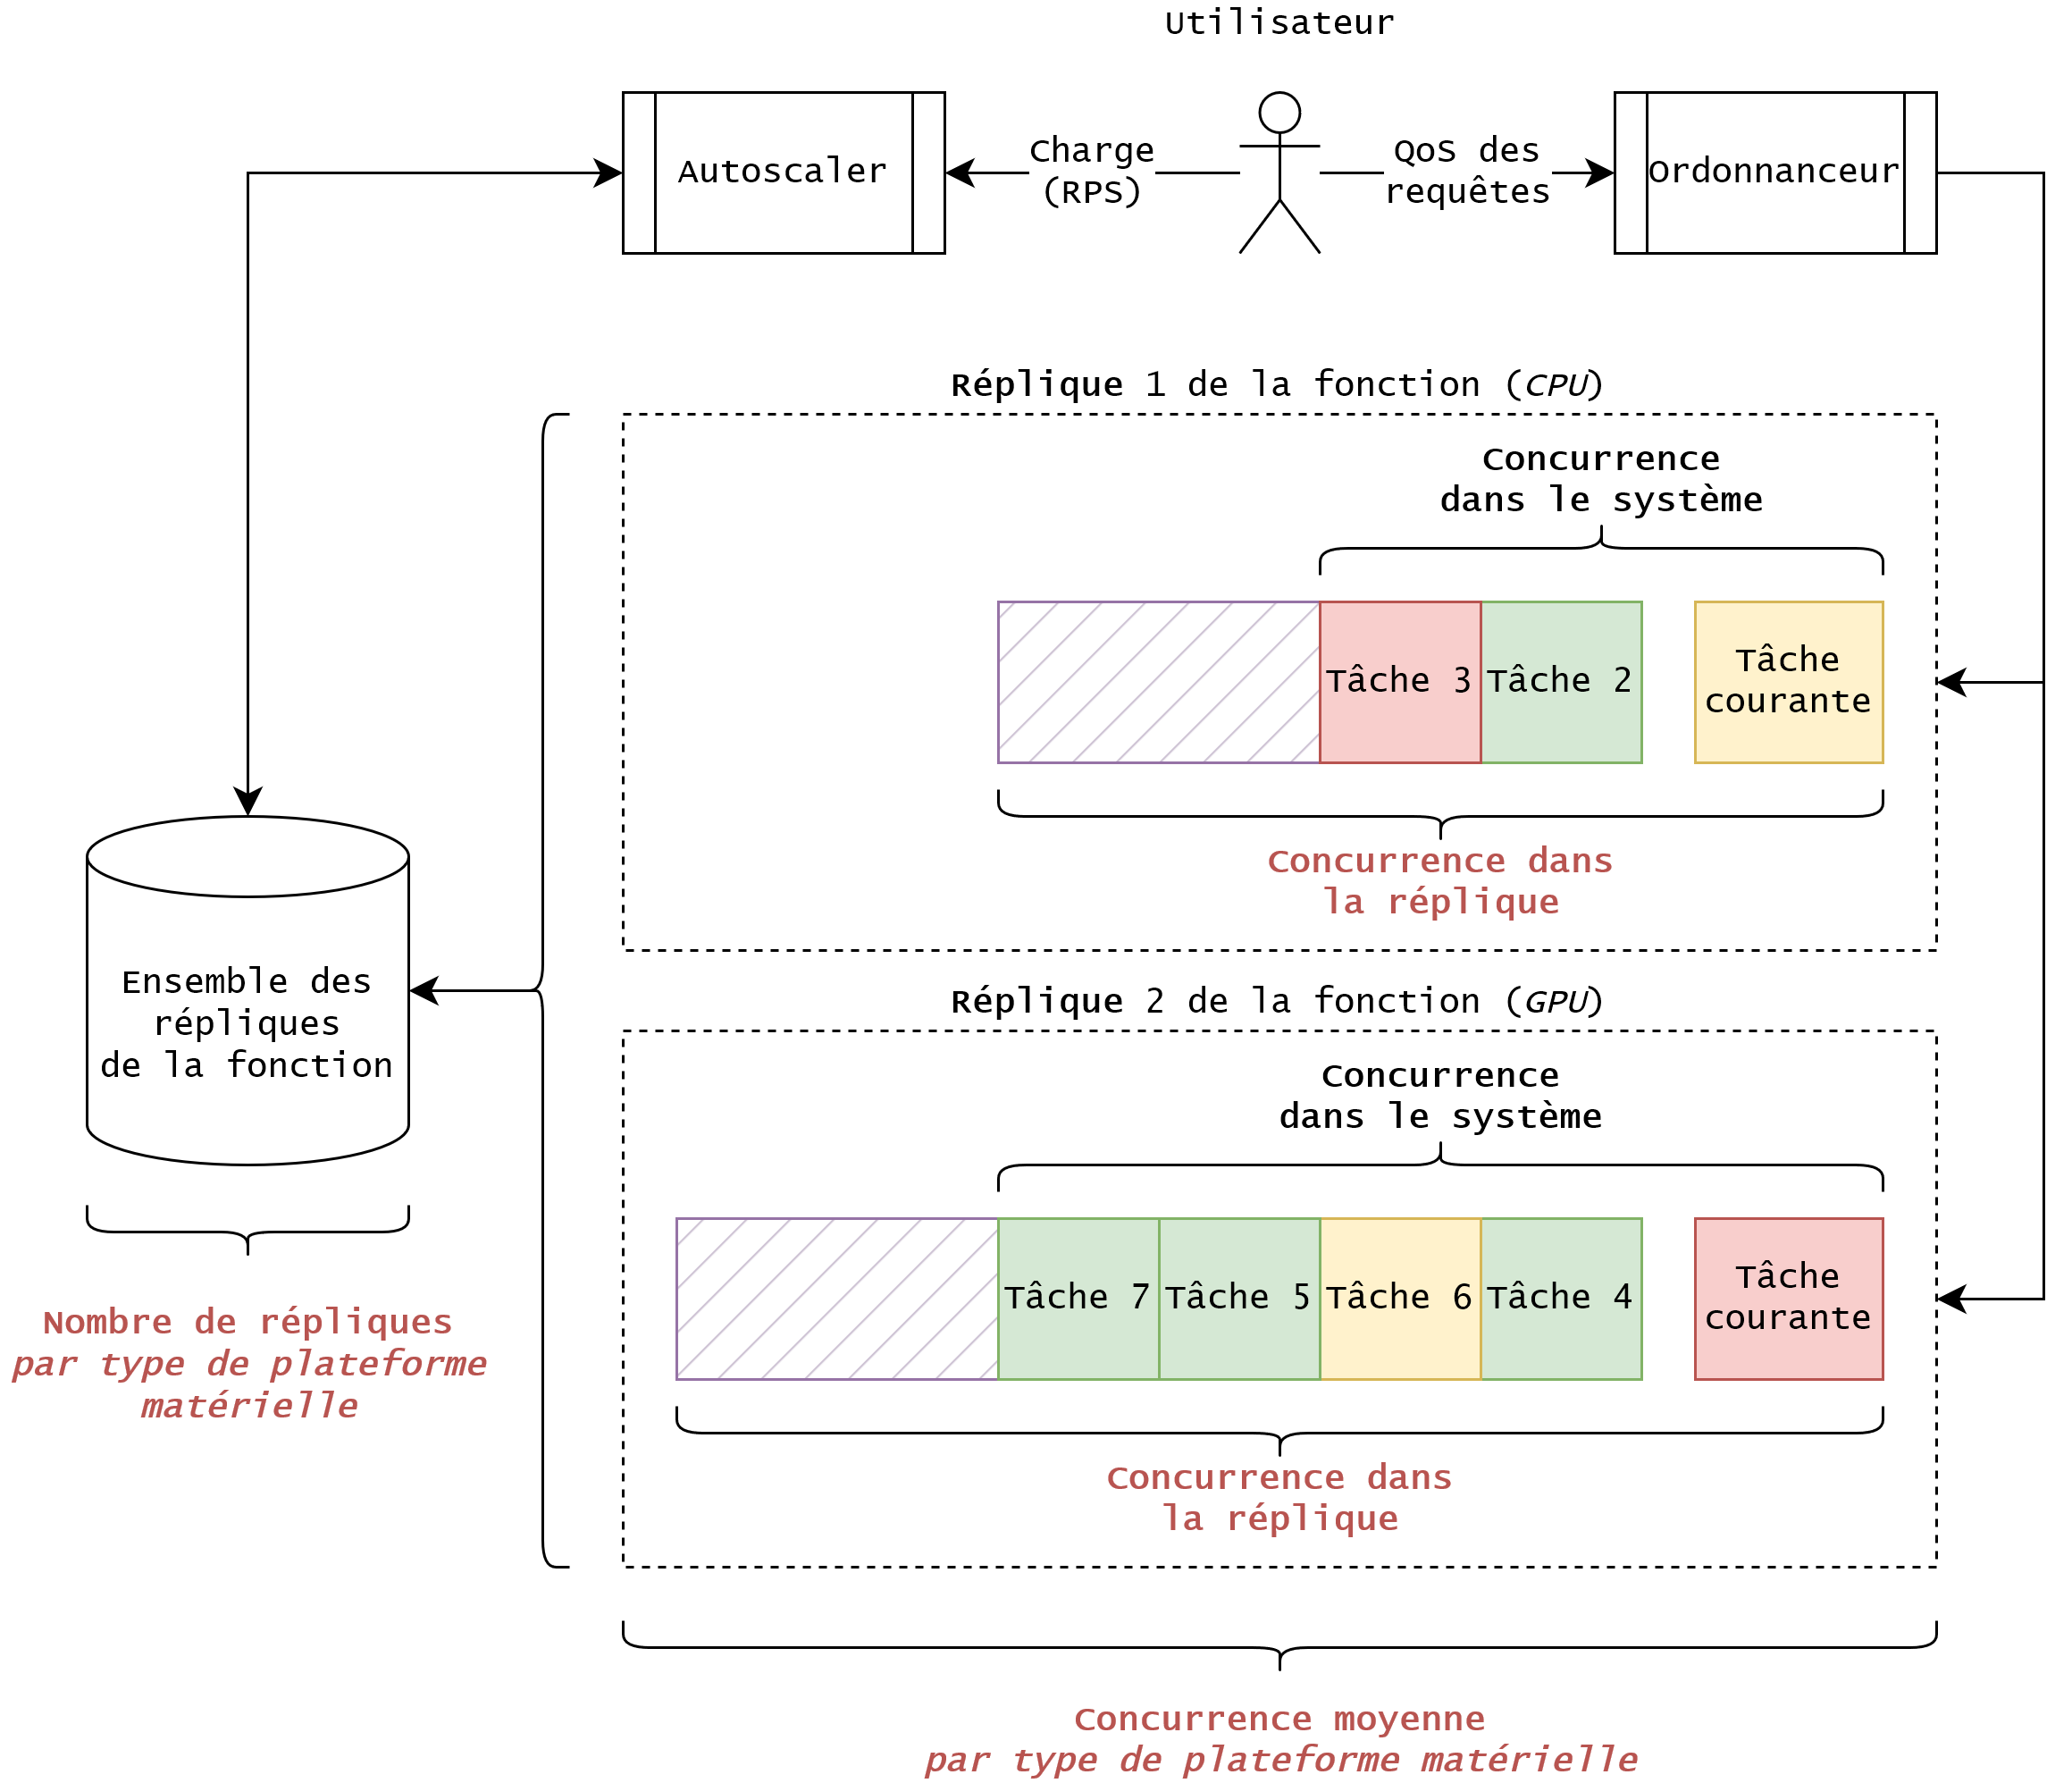
\includegraphics[width=0.9\textwidth]{4_Chapitre4/figures/orchestration-scaling.png}
    \caption{Détermination par l'autoscaler du nombre de répliques pour une fonction donnée, en prenant en compte l'hétérogénéité matérielle.}
    \label{figure:herofake-orchestration-scaling}
\end{figure}

\begin{equation}
    replicaCount_{f, h} = \frac{concurrency_{f, h}}{x_{f, h}}
\label{eq:herofake-HRO-replica-count}
\end{equation}

Une décision d'autoscaling peut introduire des coûts d'opportunité dans le système : les accélérateurs matériels sont peu disponibles par rapport aux \gls{CPU}, et le fait de les allouer à une fonction donnée à un moment donné les rendra indisponibles pour d'autres tâches. Pour que l'autoscaler puisse décider quand il est pertinent d'allouer de tels accélérateurs, il doit être \textbf{conscient des coûts}.

Afin de déterminer le seuil de concurrence par réplique, noté $x_{f, h}$ pour une fonction $f$ sur un type de matériel $h$ (par exemple, \gls{GPU} et \gls{FPGA}), nous avons fixé le seuil de concurrence par réplique sur les \gls{CPU} à $x_{f, c} = 100$, en accord avec la valeur par défaut dans Knative~\footnote{\href{https://knative.dev/docs/serving/autoscaling/concurrency/}{https://knative.dev/docs/serving/autoscaling/concurrency/}}. Ensuite, nous avons utilisé les mesures de la phase hors-ligne (tableau~\ref{table:herofake-tasks}) pour établir un ratio composite (incluant les performances, l'énergie, le prix de la plateforme) entre \gls{CPU} et accélérateurs, comme décrit dans l'équation~\ref{eq:herofake-HRO-concurrency-target}. Dans notre politique, nous avons choisi de favoriser le temps de réponse en fixant $k_{ET} = \frac{2}{3}$, $k_{EC} = \frac{1,5}{6}$ et $k_{HP} = \frac{0,5}{6}$. Par exemple, pour la fonction ResNet50 (décrite dans le tableau~\ref{model:tasks}), les files d'attente dans les répliques sont dimensionnées à 100 requêtes pour les \gls{CPU}, 489 pour les \gls{GPU} et 1292 pour les \gls{FPGA}.

\begin{equation}
    x_{f, h} = x_{f, c} \cdot (k_{ET} \cdot \frac{ET_{{f}_{c}}}{ET_{{f}_{h}}} + k_{EC} \cdot \frac{EC_{{f}_{c}}}{EC_{{f}_{h}}} + k_{HP} \cdot \frac{HP_{{f}_{c}}}{HP_{{f}_{h}}})
\label{eq:herofake-HRO-concurrency-target}
\end{equation}

Lorsque le seuil de concurrence d'une fonction est dépassé dans les files d'attente des répliques sur un type de matériel donné, l'autoscaler procède à la \textit{mise à l'échelle} (\textit{scale out}) de la fonction : une nouvelle réplique est initialisée pour traiter les nouvelles requêtes utilisateur.

L'autoscaler commence par considérer la liste complète des nœuds disponibles dans l'infrastructure. Nous commençons par constituer un sous-ensemble de \textit{nœuds appropriés} dans l'infrastructure : compte tenu des besoins en mémoire que nous avons mesurés pour chaque fonction, nous éliminons les nœuds qui ne disposent pas actuellement de suffisamment de mémoire pour héberger une réplique de la fonction. Chaque réplique déployée sur la plateforme d'exécution d'un nœud consomme la quantité totale de mémoire requise par le type de fonction. Si le nœud n'a plus de mémoire, ses plateformes d'exécution ne peuvent plus être utilisées pour déployer d'autres répliques.

Afin de sélectionner le type de ressource matérielle à allouer à cette réplique, l'autoscaler minimise la fonction de coût donnée dans l'équation~\ref{eq:herofake-HRO-allocation-cost-function}. Dans notre politique d'ordonnancement, comme pour l'autoscaling, nous avons choisi de favoriser le temps total d'exécution des tâches en fixant $k_{TT} = \frac{2}{3}$, $k_{EC} = \frac{1.5}{6}$ et $k_{HP} = \frac{0.5}{6}$.
En fonction du matériel disponible au moment de la mise à l'échelle, l'autoscaler favorisera la création d'une nouvelle réplique de fonction sur la plateforme qui exécutera la tâche dans le temps total le plus court, incluant le démarrage à froid, avec la consommation d'énergie la plus faible et le prix le plus bas.

\begin{equation}
\begin{split}
    scaleCost_{{f}_{N, P}} = \, &k_{TT} \cdot {TT}_{{f}_{N, P}} \\
    + &k_{EC} \cdot {EC}_{{f}_{N, P}} \\
    + &k_{HP} \cdot {HP}_{{f}_{N, P}}
\end{split}
\label{eq:herofake-HRO-allocation-cost-function}
\end{equation}

Au contraire, lorsque la concurrence pour une fonction tombe en dessous du seuil de concurrence sur un type de matériel donné, l'autoscaler emploiera une politique de meilleur effort et essaiera de libérer toute réplique dont la file d'attente est vide sur ce type de matériel (\textit{scale in}). Si une réplique a une file d'attente vide, sa plateforme d'exécution sera remise dans le stock de plateformes disponibles et la mémoire qui avait été allouée à la réplique sur le nœud sera libérée.

Les différents poids ($k$) utilisés dans les équations~\ref{eq:herofake-HRO-concurrency-target} et~\ref{eq:herofake-HRO-allocation-cost-function} peuvent être modifiés par le fournisseur afin de personnaliser la politique d'allocation en fonction de ses contraintes et priorités.

\subsection{Stratégie d'ordonnancement} \label{section:herofake-scheduling-strategy}

La caractérisation de la charge de travail est essentielle à la prédiction des performances. Cette prédiction guide des décisions d'ordonnancement qui pourront conduire à la satisfaction des exigences de qualité de service~\cite{mampageHolisticViewResource2022}. Notre stratégie d'ordonnancement s'appuie sur les métadonnées des tâches décrites dans la section~\ref{model:tasks}. L'acquisition de connaissances sur les tâches serverless est réalisée au cours d'une phase hors-ligne sur notre plateforme : cela est possible car le code des fonctions est poussé par les développeurs vers un magasin de fonctions en amont de leur exécution~\cite{shahradServerlessWildCharacterizing}.

Dans Knative, l'ordonnanceur gère les requêtes entrantes de manière \gls{FIFO} (pour \textit{First In, First Out}, c'est-à-dire dans leur ordre d'arrivée). Pour gérer les différents niveaux d'exigences en matière de qualité de service, nous proposons que notre ordonnanceur retire les tâches de la file d'attente de l'orchestrateur par \textbf{échéance la plus proche} (ou \gls{EDF}, pour \textit{Earliest Deadline First}). Nous calculons l'échéance de la tâche en utilisant son pire temps d'exécution à l'aide de l'équation~\ref{eq:herofake-task-wcet}, et en la multipliant par le facteur de ralentissement fixé par le niveau de qualité de service. Après l'exécution de la tâche, nous vérifierons si nous avons dépassé son échéance et fixerons la pénalité associée en conséquence, comme décrit dans l'équation~\ref{eq:herofake-task-penalty}. 

Nous itérons sur les répliques de la fonction pour calculer les métriques suivantes en s'appuyant sur ses métadonnées :

\begin{itemize}
    \item \textbf{pénalité potentielle} : on récupère la longueur de la file d'attente de la plateforme et on vérifie si l'échéance de la tâche sera dépassée, comme décrit dans l'équation~\ref{eq:herofake-task-penalty} ;
    \item \textbf{consommation d'énergie} : on récupère les mesures hors-ligne pour établir la consommation d'énergie dynamique de cette tâche sur la plateforme ;
    \item \textbf{consolidation des tâches} : on récupère la longueur $Q$ de la file d'attente de la plateforme en additionnant les durées totales de toutes les tâches en file d'attente, comme décrit dans les équations~\ref{eq:herofake-HRO-scheduling-platform-queue} (longueur de la file d'attente) et~\ref{eq:herofake-HRO-total-time} (durée totale de la tâche).
\end{itemize}

\begin{equation}
    len \, Q_{N, P} = \sum TT_{f_{N, P}}
\label{eq:herofake-HRO-scheduling-platform-queue}
\end{equation}

Ces valeurs sont normalisées pour les adapter à la fonction de coût pondérée décrite dans l'équation~\ref{eq:herofake-HRO-scheduling-cost-function}.

Pour la pondération, nous avons utilisé $k_{QP} = \frac{2}{3}$, $k_{EC} = \frac{0.5}{6}$ et $k_{TC} = \frac{1.5}{6}$ (comme pour l'autoscaler). L'ordonnanceur minimise ensuite cette fonction de coût pour toutes les répliques $(N, P)$ (c'est-à-dire l'ensemble des couples possibles de nœud $N$ et de plateforme d'exécution $P$).

\begin{equation}
\begin{split}
    schedCost_{{f}_{N, P}} = \, &k_{QP} \cdot QP_{{f}_{N, P}} \\
    + &k_{EC} \cdot {EC}_{{f}_{N, P}} \\
    + &k_{TC} \cdot TC_{{f}_{N, P}}
\end{split}
\label{eq:herofake-HRO-scheduling-cost-function}
\end{equation}

Si l'ordonnanceur ne trouve pas de réplique disponible pour exécuter la tâche, celle-ci sera remise en file d'attente au niveau de l'orchestrateur. Cela augmentera la concurrence dans le système pour la fonction, poussant l'autoscaler à allouer une autre réplique sur le matériel approprié.

\section{Évaluation}
\label{section:herofake-evaluation}

Dans cette section, nous détaillons notre méthodologie pour l'évaluation de notre politique d'orchestration dans un environnement de simulation. Nous la comparons à des politiques de référence et de l'état de l'art, et nous montrons l'impact de ses composants individuels sur la performance globale.

\subsection{Protocole expérimental}

Nous avons utilisé des mesures provenant de l'évaluation de trois modèles d'apprentissage différents (voir tableau~\ref{table:herofake-tasks}). Ces modèles ont été mis en œuvre sur trois plateformes d'exécution différentes (voir tableau~\ref{table:herofake-platforms}) comme expliqué dans la section~\ref{section:herofake-offline}.

Ces données ont servi en entrée à un simulateur à évènements discrets que nous avons développé et publié sous licence libre. Le simulateur suit le modèle décrit dans les sections~\ref{model:nodes}, \ref{model:platforms}, et \ref{model:tasks}. De plus amples détails sont donnés dans le voir chapitre~\ref{chapter:herosim}.

Nous avons mesuré les délais de démarrage à froid pour les applications de notre étude de cas (tableau~\ref{table:herofake-tasks}). Il apparaît que les temps d'exécution pour les fonctions considérées sont dominés par les délais de démarrage à froid, ce qui fait de l'allocation adéquate des ressources une exigence stricte pour respecter les accords de niveau de service.

Dans la partie consacrée à l'évaluation des performances, nous comparons deux autoscalers :

\begin{itemize}
    \item HeROfake (HRO) -- Notre allocateur de ressources basé sur les métadonnées et conscient de l'hétérogénéité matérielle ;
    \item Knative (KN) -- Nous avons modélisé le comportement de l'autoscaler de Knative du mieux que nous avons pu, en nous appuyant sur la documentation disponible au moment de cette étude~\footnote{\href{https://knative.dev/docs/serving/autoscaling/}{https://knative.dev/docs/serving/autoscaling/}}.
\end{itemize}

Notre évaluation comporte quatre ordonnanceurs :

\begin{itemize}
    \item HeROfake (HRO) -- Notre ordonnanceur conscient des coûts qui minimise les violations de \gls{SLA}, la consommation d'énergie et la quantité totale de ressources engagées ;
    \item Knative (KN) -- Knative sélectionne une réplique sur le nœud le plus disponible~\cite{sureshENSUREEfficientScheduling2020}. Les répliques sont triées en fonction du nombre de requêtes en cours de traitement. La réplique avec la file d'attente la plus courte est sélectionnée ;
    \item Random Placement (RP) -- Les tâches sont assignées à une réplique aléatoire sur un nœud aléatoire ;
    \item Bin Packing First-Fit (\gls{BPFF}) -- Les tâches sont consolidées sur un nombre minimum de répliques. L'ordonnanceur place les requêtes sur une première réplique jusqu'à ce que celle-ci atteigne son seuil de concurrence. \gls{BPFF} est la politique d'ordonnancement mise en œuvre pour \gls{AWS} Lambda~\cite{wangPeekingCurtainsServerlessb}.
\end{itemize}

Nous avons conçu une évaluation des performances en deux étapes basée sur des simulations :

\begin{itemize}
    \item \textbf{Comparaison aux politiques de référence} (figure~\ref{figure:herofake-evaluation-hro-full}) : dans cette partie, nous avons comparé notre combinaison d'autoscaler et d'ordonnanceur, HeROfake (HRO-HRO), à : (1) l'autoscaler et l'ordonnanceur Knative complet (KN-KN), (2) l'autoscaler Knative avec l'ordonnanceur \gls{BPFF} (KN-BPFF), (3) l'autoscaler Knative avec l'ordonnanceur RP (KN-RP) ;
    \item \textbf{Impact des composants sur la performance globale} (figure~\ref{figure:herofake-evaluation-hro-mixed}) : nous discutons ici de l'impact individuel de chacun des autoscalers et ordonnanceurs. Pour ce faire, nous avons conçu différentes stratégies : (1) en utilisant l'autoscaler HeROfake avec l'ordonnanceur Knative (HRO-KN), et (2) en utilisant l'autoscaler Knative avec l'ordonnanceur HeROfake (KN-HRO), puis nous avons comparé ces stratégies avec les versions complètes de HeROfake (HRO-HRO) et Knative (KN-KN).
\end{itemize}

La dénomination de chaque scénario dans ces figures se compose de deux parties séparées par un délimiteur. La première partie correspond à la politique d'allocation, la seconde à la politique d'ordonnancement (par exemple, HRO-KN signifie que nous avons utilisé l'autoscaler HeROfake en conjonction avec l'ordonnanceur Knative).

Pour chacune des combinaisons de politiques d'autoscaler et d'ordonnanceur, nous avons réalisé l'expérience sur la base d'un scénario à charge de travail synthétique, composée de 50000 tâches (requêtes utilisateur). Les tâches se voient attribuer un type aléatoire (ResNet50, VGG16 ou VGG19) et un niveau de \gls{QoS} aléatoire (élevé, moyen, faible) suivant une distribution uniforme, avec des facteurs de ralentissement pour la \gls{QoS} respectivement fixés à 2, 3 et 4. L'infrastructure du scénario se compose de 10 nœuds sur lesquels sont réparties 18 plateformes d'exécution (10 \gls{CPU}, 6 \gls{GPU}, 2 \gls{FPGA}).

Les pondérations pour le niveau de concurrence (équation~\ref{eq:herofake-HRO-concurrency-target}) ont été fixées à $k_{ET} = \frac{2}{3}$, $k_{EC} = \frac{1,5}{6}$ et $k_{HP} = \frac{0,5}{6}$. Les pondérations pour la décision de mise à l'échelle (équation~\ref{eq:herofake-HRO-allocation-cost-function}) ont été fixées à $k_{TT} = \frac{2}{3}$, $k_{EC} = \frac{1,5}{6}$ et $k_{HP} = \frac{0,5}{6}$. Les pondérations pour la décision d'ordonnancement (équation~\ref{eq:herofake-HRO-scheduling-cost-function}) ont été fixées à $k_{QP} = \frac{2}{3}$, $k_{EC} = \frac{0,5}{6}$ et $k_{TC} = \frac{1,5}{6}$.

\subsection{Analyse des résultats}

\subsubsection{Comparaison aux politiques de référence}

\begin{figure*}[!ht]
    \centering
    \subfloat[Consolidation (nombre de nœuds inutilisés)\label{figure:herofake-evaluation-full-nodes}]{
        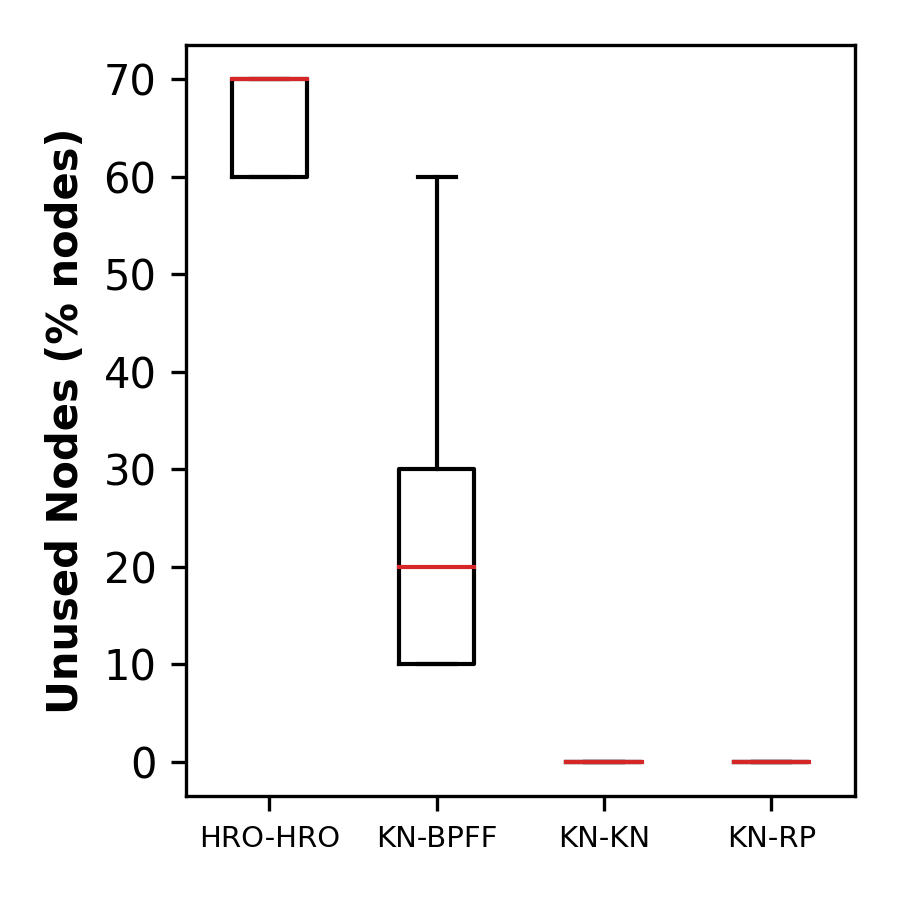
\includegraphics[width=0.28\linewidth]{4_Chapitre4/figures/evaluation/z-nodes-20221212-232143-169224.png}
    }\qquad
    \subfloat[Pénalités sur \gls{QoS} (tâches dont on rate l'échéance)\label{figure:herofake-evaluation-full-penalty}]{
        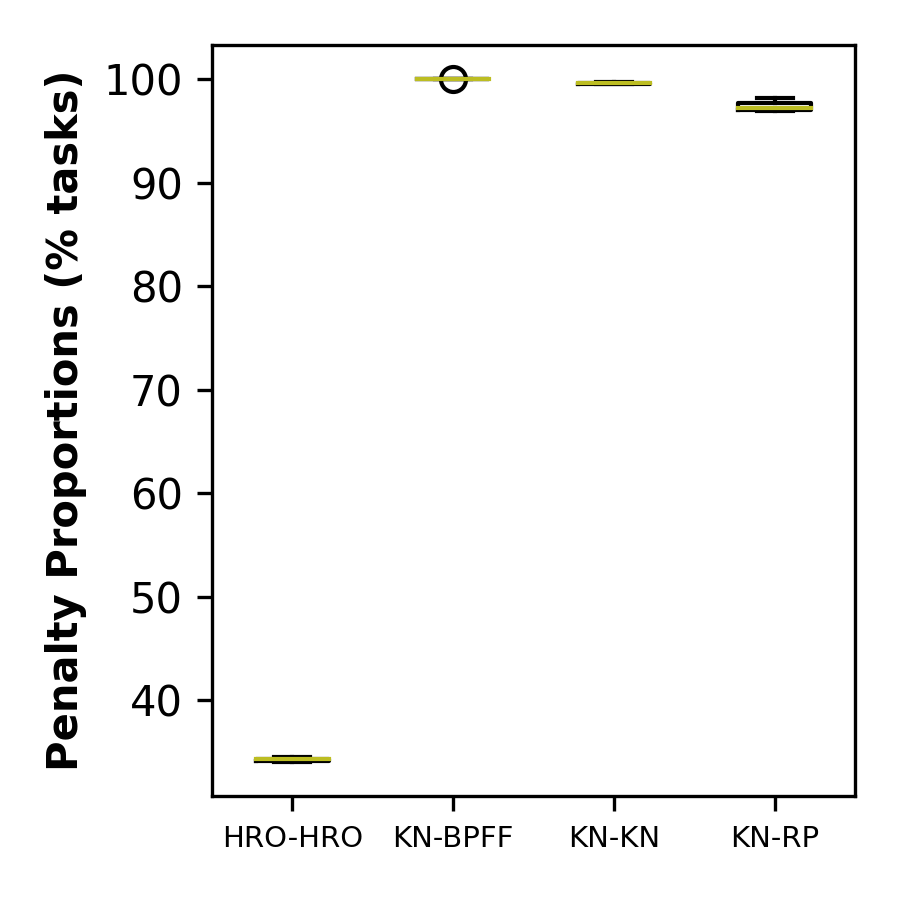
\includegraphics[width=0.28\linewidth]{4_Chapitre4/figures/evaluation/z-penalty-20221212-232143-169224.png}
    }\qquad
    \subfloat[Consommation d'énergie dynamique (exécution des tâches)\label{figure:herofake-evaluation-full-energy}]{
        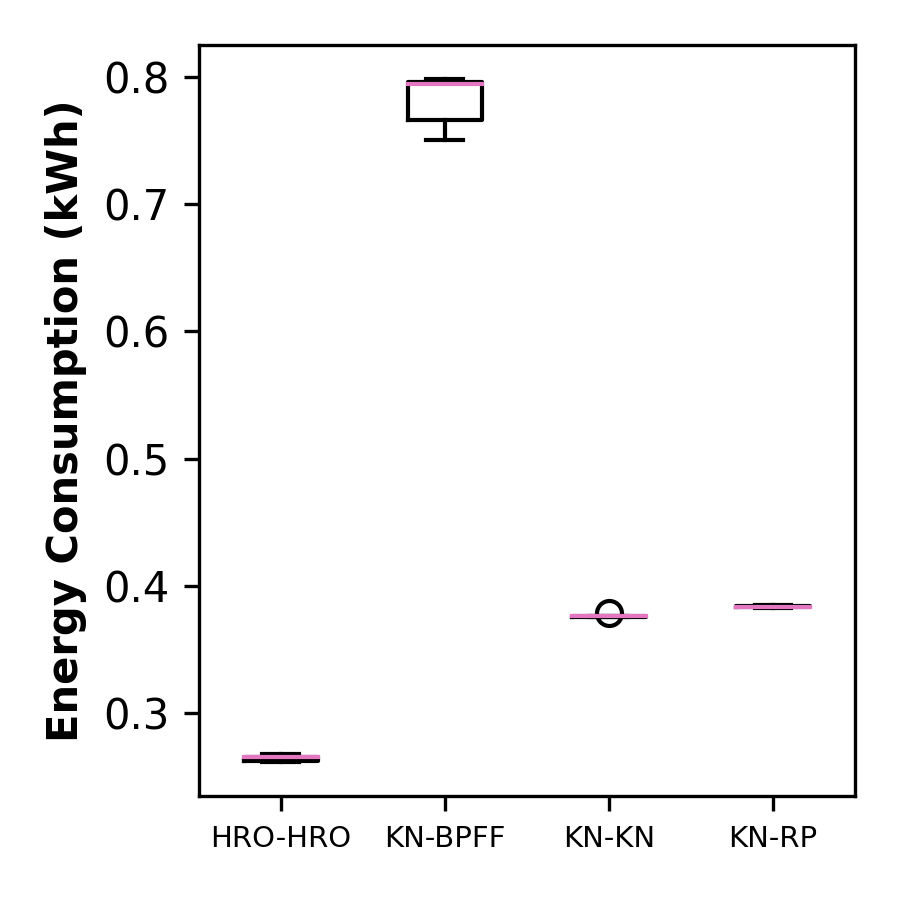
\includegraphics[width=0.28\linewidth]{4_Chapitre4/figures/evaluation/z-energy-20221212-232143-169224.png}
    }
    \caption{Évaluation 1 -- Comparaison des performances de HeROfake avec les méthodes de référence.}
    \label{figure:herofake-evaluation-hro-full}
\end{figure*}

\textbf{Consolidation des tâches}. La figure~\ref{figure:herofake-evaluation-full-nodes} montre que notre combinaison d'autoscaler et d'ordonnanceur permet d'obtenir le plus grand nombre de nœuds inutilisés. Avec l'autoscaler de Knative, l'ordonnanceur \gls{BPFF} assure la meilleure consolidation, mais cette politique nécessite toujours plus de trois fois le nombre de nœuds que nous allouons avec notre politique.

\textbf{Accords de niveau de service}. La figure~\ref{figure:herofake-evaluation-full-penalty} montre que HRO-HRO est le plus performant en termes de violations de la \gls{QoS}, avec 35\% de tâches qui ne respectent pas les délais. Il s'agit d'une amélioration considérable par rapport aux résultats de Knative, où les tâches ne respectent pas leur échéance dans plus de 99\% des cas : le retard introduit par l'allocation réactive des ressources ne peut pas être compensé à temps en utilisant uniquement des \gls{CPU}.

\textbf{Consommation d'énergie}. La figure~\ref{figure:herofake-evaluation-full-energy} montre que notre politique, avec l'autoscaler et l'ordonnanceur HRO fonctionnant conjointement, est toujours la plus performante en termes de consommation d'énergie dynamique. Cela s'explique évidemment par le fait que nous allouons des accélérateurs matériels ; cependant, au cours de notre évaluation, la durée d'exécution de notre scénario est similaire avec les politiques Knative et HRO (environ 13,5 minutes). La politique d'ordonnancement \gls{BPFF} est également la moins performante en termes de temps d'exécution, car elle maximise la taille des files d'attente dans les répliques, ce qui donne les pires résultats en termes de consommation d'énergie.

\subsubsection{Impact des composants individuels}

\begin{figure*}[!ht]
    \centering
    \subfloat[Consolidation (nombre de nœuds inutilisés)\label{figure:herofake-evaluation-mixed-nodes}]{
        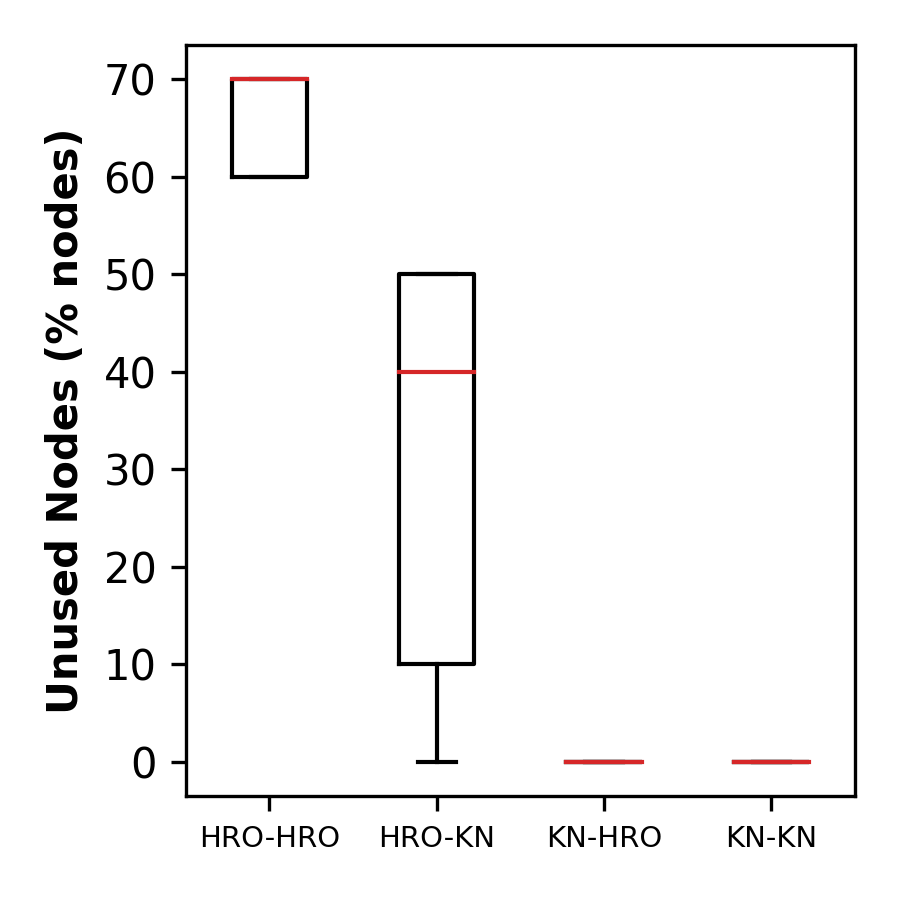
\includegraphics[width=0.28\linewidth]{4_Chapitre4/figures/evaluation/x-nodes-20221212-185844-053283.png}
    }\qquad
    \subfloat[Pénalités sur \gls{QoS} (tâches dont on rate l'échéance)\label{figure:herofake-evaluation-mixed-penalty}]{
        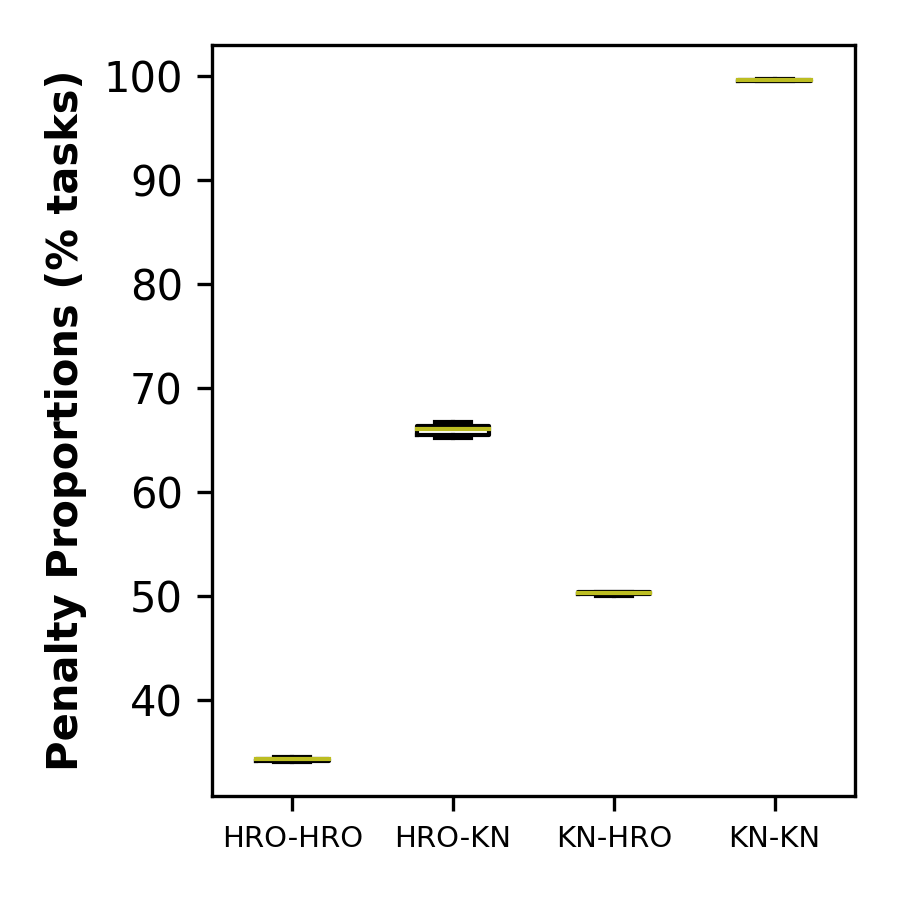
\includegraphics[width=0.28\linewidth]{4_Chapitre4/figures/evaluation/x-penalty-20221212-185844-053283.png}
    }\qquad
    \subfloat[Consommation d'énergie dynamique (exécution des tâches)\label{figure:herofake-evaluation-mixed-energy}]{
        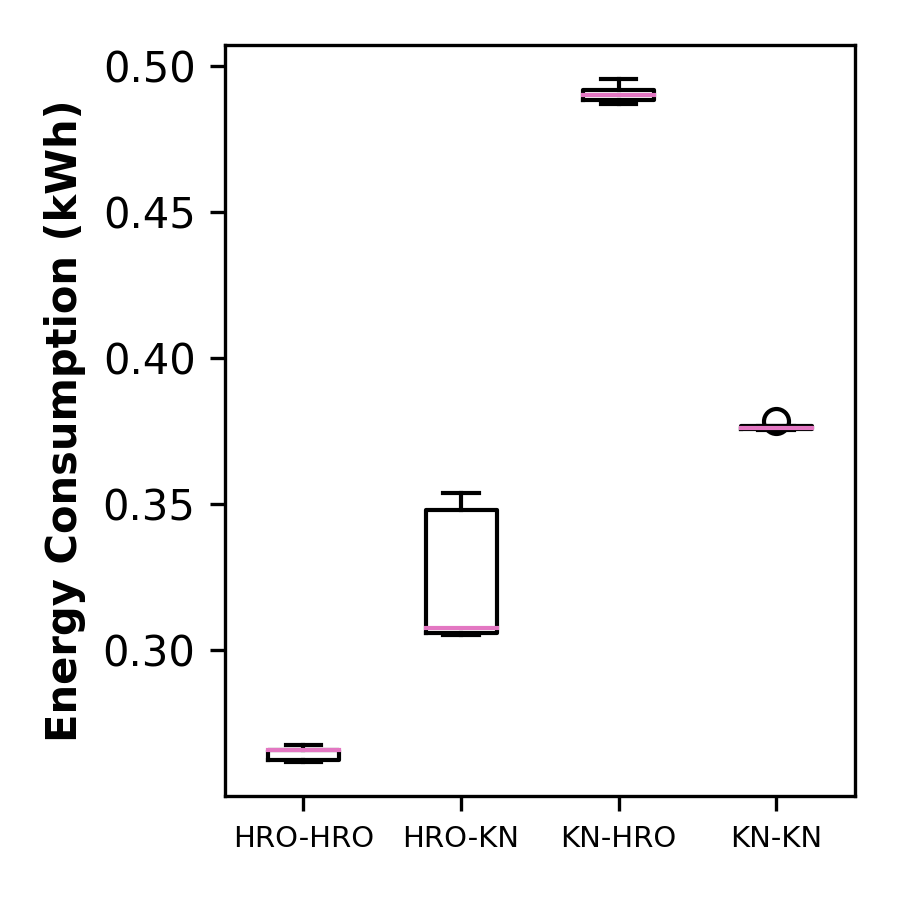
\includegraphics[width=0.28\linewidth]{4_Chapitre4/figures/evaluation/x-energy-20221212-185844-053283.png}
    }
    \caption{Évaluation 2 -- Impact des composants individuels de HeROfake sur la performance globale.}
    \label{figure:herofake-evaluation-hro-mixed}
\end{figure*}

\textbf{Consolidation des tâches}. La figure~\ref{figure:herofake-evaluation-mixed-nodes} montre que HRO-HRO est le plus performant en matière de consolidation des tâches, laissant un peu moins de 70\% des nœuds disponibles inutilisés, alors que l'ordonnanceur de Knative, dans le cadre de notre politique d'autoscaling, n'atteint que 40\% de nœuds inutilisés. Ce résultat est attendu, car l'ordonnanceur de Knative utilise une politique de répartition de charge. Les résultats de consolidation de KN-HRO sont médiocres, mais pour une raison différente : notre ordonnanceur tente de minimiser les violations de la qualité de service en répartissant la charge sur tous les processeurs alloués.

\textbf{Accords de niveau de service}. La figure~\ref{figure:herofake-evaluation-mixed-penalty} montre que notre ordonnanceur ne fonctionne pas bien en conjonction avec l'autoscaler de Knative. En effet, notre ordonnanceur tente de minimiser les pénalités : lorsqu'il ne dispose que de \gls{CPU}, il se comporte de la même manière que l'ordonnanceur de Knative et répartit les tâches sur ces \gls{CPU} afin de limiter les violations de qualité de service. Cependant, notre ordonnanceur sous l'autoscaler Knative parvient toujours à maintenir les violations de la qualité de service à environ 50\% des tâches, ce qui montre qu'il y a une marge d'amélioration même lorsque les tâches d'inférence sont déployées sur des \gls{CPU} uniquement, en jouant sur la politique de sélection des requêtes. On note que lors de notre évaluation, l'autoscaler Knative a donné les pires résultats en ce qui concerne la fréquence des démarrages à froid (6,5 fois plus fréquents avec KN-HRO qu'avec HRO-KN).

\textbf{Consommation d'énergie}. La figure~\ref{figure:herofake-evaluation-mixed-energy} montre que la consommation d'énergie est toujours plus faible lorsque l'on utilise notre autoscaler, qui peut allouer des accélérateurs matériels. En revanche, notre ordonnanceur utilisé avec l'autoscaler de Knative donne les pires résultats en termes de consommation d'énergie. Cela s'explique à nouveau par le fait que l'ordonnanceur tente de minimiser les pénalités en répartissant les tâches sur un grand nombre de \gls{CPU}, la plateforme d'exécution la plus consommatrice en énergie dans notre cas d'étude.

\section{Conclusion et perspectives}
\label{section:herofake-conclusion}

Dans ce chapitre, nous avons présenté HeROfake, notre politique pour le déploiement de tâches de détection de deepfake, basées sur des fonctions interactives et de courte durée, sur un cloud privé hétérogène dans le modèle serverless.

Nous avons présenté les deux phases qui composent le cadre de notre politique : une phase hors-ligne au cours de laquelle nous caractérisons les performances des plateformes d'exécution et les exigences des fonctions ; et une phase en ligne au cours de laquelle nous allouons dynamiquement les ressources et ordonnançons les tâches à exécuter sur ces plateformes.

Avec notre politique d'allocation et d'ordonnancement, la plateforme est en mesure de traiter \num{50000} tâches dans le même laps de temps que Knative, avec moins de 36\% de pénalités de \gls{QoS}. Notre stratégie réduit la consommation d'énergie dynamique pour l'exécution des tâches de près de 35\%, et permettrait au fournisseur de réduire davantage la consommation d'énergie statique en consolidant les tâches sur moins de 29\% des nœuds disponibles.

L'inclusion du traitement vidéo dans la plateforme est un défi intéressant, car il introduirait des dépendances entre les tâches. Les exécutions de fonctions ne seraient plus \textit{sans état}, ce qui entraînerait la nécessité de s'intéresser au problème du stockage des données intermédiaires dans une infrastructure serverless.

C'est l'objet du chapitre suivant, dans lequel nous traitons un nouveau cas d'étude qui concerne le déploiement d'applications complexes, composées de tâches interdépendantes.


\clearemptydoublepage
\chapter{HeROcache : Applications serverless et coûts associés aux systèmes de stockage}
\label{chapter:herocache}

\section{Introduction}
\label{section:herocache-introduction}

Dans le chapitre précédent, nous avons vu comment allouer dynamiquement des ressources matérielles et ordonnancer les requêtes utilisateur dans une plateforme serverless pour des applications simples, composées d'une unique fonction, sous contrainte de qualité de service. Un défi important dans le paradigme serverless, lorsque l'on souhaite garantir la qualité de service pour les utilisateurs, survient lors de la composition des fonctions~\cite{burckhardtNetheriteEfficientExecution}. Ce mécanisme consiste à chaîner des appels de fonctions pour réaliser des tâches complexes, qui induisent des dépendances temporelles et de données. Une chaîne de fonctions est appelée \textit{application} (parfois \textit{workflow}~\footnote{\href{https://cloud.google.com/workflows}{https://cloud.google.com/workflows}}). Au cours de l'exécution d'une telle application, les fonctions qui la composent peuvent être instanciées sur tout nœud de l'infrastructure par la plateforme serverless. Leur initialisation provoque des temps de démarrage à froid, et leur dispersion sur les nœuds génère des délais de communication qui s'additionnent tout au long de la chaîne, dégradant ainsi la qualité de service requise par les différents utilisateurs.

\boitemagique{Question 2 (\textbf{QR2})}{
    Comment déployer des applications complexes, composées de chaînes de fonctions de courte durée, et comment tirer parti de l'hétérogénéité des nœuds disponibles à l'edge, pour respecter la qualité de service requise par les utilisateurs tout en contenant la consommation d'énergie de l'infrastructure ?
}

Le problème que nous abordons dans ce chapitre est celui de la prise en compte par une plateforme serverless des délais d'initialisation et de communication dans des chaînes de fonctions de courte durée de vie.
Dans le contexte serverless, ces délais peuvent dominer le temps d'exécution total d'une application si elle se compose de fonctions de courte durée~\cite{yanHermesEfficientCache2020}, qui représentent une part non négligeable des charges de travail serverless (voir section~\ref{section:herocache-background}).

Le cadre applicatif présenté dans ce chapitre est lié à un projet \gls{AID}~\footnote{\href{https://www.defense.gouv.fr/aid}{https://www.defense.gouv.fr/aid}} (Agence de l'Innovation de Défense) visant à optimiser le déploiement de systèmes de détection d'intrusion (\gls{IDS}, pour \textit{Intrusion Detection Systems}) sur des plateformes embarquées~\cite{SLIMANI2024}. L'application considérée est critique et composée de plusieurs briques logicielles, dont les durées d'exécution sont courtes, et qui communiquent entre elles ; la plateforme matérielle envisagée est hétérogène, et présente des limites en termes de capacité et de performances qui rendent saillants les problèmes soulevés.

Pour déployer des applications sensibles au temps composées de fonctions à courte durée de vie dans un contexte edge, hétérogène et serverless, trois défis doivent être relevés : (1) réduire les délais d'initialisation, (2) éviter des délais de communication élevés et (3) exploiter des ressources hétérogènes pour satisfaire une \gls{QoS} variable :

\begin{enumerate}
    \item \textbf{Délais d'initialisation.} Le serverless s'appuyant sur des ressources non réservées, l'initialisations des fonctions, nécessitant de récupérer leur image depuis un support distant vers les nœuds edge, peut dégrader la latence des requêtes~\cite{yanHermesEfficientCache2020}, surtout dans le cas de fonctions de courte durée comme dans l'\gls{IDS} -- d'autant plus que les dispositifs edge exposent des supports de stockage de faible capacité et de faible performance, derrière des liaisons réseau limitées en termes de fiabilité et de vitesse.
    \item \textbf{Délais de communication.} Dans une infrastructure distribuée telle que le serverless à l'edge, les fonctions d'une même application peuvent être déployées sur plusieurs nœuds éloignés les uns des autres. Cela implique l'utilisation du réseau, pour exploiter un support de stockage distant lorsque ces fonctions ont besoin de communiquer des résultats intermédiaires. Ces communications par un stockage lent entraînent des retards qui peuvent conduire à des violations de la qualité de service~\cite{wawrzoniakBoxerDataAnalytics2021a}.
    \item \textbf{Hétérogénéité matérielle}. La plateforme serverless ne peut pas considérer tous les placements de tâches comme égaux, car ils produiront différents niveaux de performance : certaines plateformes matérielles sont plus adaptées à certaines tâches. Cependant, l'affinité d'une fonction avec une plateforme d'exécution spécifique ne peut pas guider à elle seule les décisions d'ordonnancement, car ces fonctions peuvent appartenir à différentes chaînes en fonction de l'application demandée. Un placement qui ne prend pas en considération la chaîne de fonctions dans laquelle la requête s'inscrit risque d'entraîner des violations de \gls{QoS}.
\end{enumerate}

\begin{table*}[!ht]
    \centering
        \caption{État de l'art des plateformes d'orchestration prenant en compte les données.}
        \resizebox{\textwidth}{!}{
            \begin{tabular}{lYYYYYYY}
                \toprule
                & Chaînes de fonctions & \gls{QoS} par requête & Hétérogénéité matérielle & Contrainte de programmation & Énergie & Cache de fonctions & {Com- \newline munications} \\
                \cmidrule(lr){2-2}\cmidrule(lr){3-3}\cmidrule(lr){4-4}\cmidrule(lr){5-5}\cmidrule(lr){6-6}\cmidrule(lr){7-7}\cmidrule(lr){8-8}
                Cypress~\cite{bhasiCypressInputSizesensitive2022} & \cmark & \cmark & \xmark & \cmark & \cmark & \xmark & \cmark \\
                FaDO~\cite{smithFaDOFaaSFunctions2022} & \xmark & \xmark & \xmark & \cmark & \xmark & \xmark & \cmark \\
                FaasFlow~\cite{zijunFassflowEfficient2022} & \cmark & \xmark& \xmark & \xmark & \xmark & \xmark & \xmark \\
                FIRST~\cite{zhangFIRSTExploitingMultiDimensional2023} & \xmark & \xmark & \xmark & \cmark & \cmark & \xmark & \xmark \\
                HeROfake~\cite{herofake} & \xmark & \cmark & \cmark & \cmark & \cmark & \xmark & \xmark \\
                Netherite~\cite{burckhardtNetheriteEfficientExecution} & \cmark & \xmark & \xmark & \cmark & \xmark & \xmark & \cmark \\
                Palette~\cite{abdiPaletteLoadBalancing2023} & \cmark & \xmark & \xmark & \xmark & \xmark & \cmark & \cmark \\
                Solution cible & \cmark & \cmark & \cmark & \cmark & \cmark & \cmark & \cmark \\
                \bottomrule
            \end{tabular}
        }
    \label{table:herocache-sota}
\end{table*}

Des études antérieures ont exploré le besoin de plateformes d'orchestration qui prennent en charge l'ordonnancement de chaînes de fonctions sur des ressources non réservées. Le tableau~\ref{table:herocache-sota} résume dans quelle mesure ces solutions ne sont pas applicables à notre étude de cas ; le chapitre~\ref{chapter:sota} donne plus de détails en section~\ref{section:sota-herocache}. Ces contributions visent généralement les déploiements dans le cloud, où l'enjeu est de traiter autant de tâches que possible dans une infrastructure homogène de nœuds toujours en service, afin de maximiser l'utilisation des ressources. L'objectif de notre étude est de montrer qu'avec des politiques d'allocation et d'ordonnancement adéquates, nous pouvons déployer des applications bien définies sur un nombre limité de nœuds hétérogènes et réduire ainsi la consommation d'énergie globale de l'infrastructure en consolidant les tâches connexes.

Dans ce chapitre, nous présentons une solution qui s'appuie sur trois axes pour répondre aux trois défis mentionnés plus haut. HeROcache (1) exploite un mécanisme de mise en cache sur les nœuds edge qui réduit \textbf{les délais d'initialisation} sans saturer leur capacité de stockage ; (2) consolide les tâches sur la base d'une application afin de limiter la durée des \textbf{délais de communication} entre les fonctions ; (3) gère le respect des exigences de qualité de service pour les tâches critiques en utilisant des métadonnées collectées auprès des applications et des plateformes hétérogènes utilisées pour le déploiement. Ces données comprennent des mesures de performance et d'énergie qui guident l'orchestrateur dans ses prises de décision, lors de l'allocation de ressources et de l'ordonnancement de requêtes toutes \textbf{hétérogènes}.

Le chapitre est organisé comme suit : la section~\ref{section:herocache-background} détaille les défis pour le déploiement de l'\gls{IDS} sur une plateforme serverless ; la section~\ref{section:herocache-before-contrib} présente le projet et son architecture globale ; la section~\ref{section:herocache-workload} détaille notre approche de collecte de métadonnées hors-ligne ; la section~\ref{section:herocache-contribution} décrit notre stratégie d'orchestration en ligne ; la section~\ref{section:herocache-evaluation} discute des résultats de l'évaluation ; enfin, la section~\ref{section:herocache-conclusion} conclut le chapitre en donnant des limites à cette contribution et des perspectives pour de futurs travaux.

\section{Contexte et motivation}
\label{section:herocache-background}

Dans cette section, nous motivons le déploiement d'applications d'\gls{IDS} sur des dispositifs \textit{edge}, en particulier sur une plateforme serverless. Nous détaillons ensuite les défis à relever pour optimiser un tel déploiement pour la \gls{QoS} sous contrainte d'énergie. Nous montrons que les délais d'initialisation et de communication entre les fonctions sont particulièrement critiques dans le cas de nos applications.

\subsection{Détection d'intrusion à l'edge}

Un large éventail de systèmes embarqués fonctionnant dans des environnements statiques et contrôlés (capteurs dans une usine) ou dynamiques et non contrôlés (essaims de drones en mouvement) peuvent être temporairement ou constamment exposés à des attaques critiques par l'intermédiaire de liaisons réseau. Comme ces attaques peuvent compromettre leur exécution et endommager gravement les infrastructures connexes, il est essentiel de les prendre en compte. Pour atténuer ces menaces, les systèmes de détection d'intrusion sont utilisés pour analyser le trafic réseau et détecter des motifs d'activités potentiellement malveillantes. Les modèles d'apprentissage machine sont particulièrement utiles pour classifier ce trafic, mais ils sont très gourmands en ressources de calcul, en mémoire et en stockage. Par conséquent, les exécuter directement sur la plateforme embarquée n'est pas une solution sûre, car cela peut affecter leur durée de vie s'ils fonctionnent sur batterie~\cite{slimani:hal-04159551}, interférer avec d'autres tâches critiques, ou même être totalement impossible en raison d'un manque de ressources.

Pour décharger les systèmes embarqués de l'exécution de ces algorithmes gourmands en ressources, tout en maintenant le système réactif aux attaques, une solution consiste à exécuter les \gls{IDS} dans le cloud, et en particulier sur les dispositifs \textit{edge}~\cite{eskandari2020}. Les \gls{IDS} doivent répondre à des exigences variables en matière de qualité de service et peuvent n'être nécessaires que pendant des périodes critiques, identifiées à l'avance. En outre, différents types d'attaques peuvent présenter des risques différents sur l'infrastructure sous-jacente, et le risque d'attaque peut varier dans le temps et dans l'espace (en fonction du domaine d'application). Par conséquent, il pourrait être inutilement coûteux de déployer des systèmes de détection d'intrusion sur des dispositifs edge réservés. Nous soutenons que le déploiement d'\gls{IDS} sur des ressources non réservées à faible consommation d'énergie à l'edge pourrait offrir l'avantage d'une solution rentable pour l'exécution de telles applications, tout en offrant une latence plus faible que lorsque l'on s'appuie sur le cloud.

\subsection{Orchestration dynamique d'applications critiques à l'edge}

L'un des principaux paradigmes du cloud qui permet d'exécuter des applications interactives sur des ressources non réservées, avec une granularité fine d'allocation des ressources, est le serverless~\cite{Lannurien2023}. Le déploiement serverless à l'edge pour l'\gls{IDS}, et plus généralement pour les applications critiques et sensibles au temps, peut être intéressant du point de vue des coûts car il ouvre des possibilités d'optimisation pour le fournisseur de services, grâce à la mise à l'échelle dynamique des ressources suite à des pics de charge dans les applications interactives, ainsi qu'à la granularité d'allocation fine et mesurée pour les ressources limitées à l'edge.

Lorsqu'un événement déclenche leur exécution, les fonctions sont déployées sur des nœuds de l'infrastructure, dans des environnements d'exécution appelés \textbf{répliques}. Comme les fonctions sont sans état, les requêtes peuvent être attribuées à n'importe quelle réplique disponible. La mise à l'échelle d'une application serverless, \textit{i.e.} pour maintenir un niveau de performance constant, consiste à faire croître ou décroître le nombre de répliques des fonctions en suivant les pics de charge. Les plateformes serverless basées sur Kubernetes, telles que Knative~\footnote{\href{https://knative.dev/}{https://knative.dev/}} ou OpenWhisk~\footnote{\href{https://openwhisk.apache.org/}{https://openwhisk.apache.org/}}, ont proposé un modèle basé sur un seuil de concurrence pour le dimensionnement du nombre de répliques. Pour toute fonction, un \textbf{autoscaler} peut déployer plusieurs \textit{répliques} pour absorber la charge. Chaque réplique est allouée à une plateforme d'exécution (\textit{i.e.} un cœur de \gls{CPU}, un \gls{GPU}, etc.) et dispose d'une file d'attente pour les requêtes entrantes. Le nombre de répliques pour une fonction donnée à un instant donné détermine son niveau de concurrence. Un \textbf{ordonnanceur} place les requêtes utilisateur dans la file d'attente d'une réplique de la fonction.

Une étude récente a montré que 50\% des applications serverless déployées sur Microsoft Azure Durable Functions~\footnote{\href{https://learn.microsoft.com/en-US/azure/azure-functions/durable/durable-functions-overview}{https://learn.microsoft.com/en-US/azure/azure-functions/durable/durable-functions-overview}} sont constituées de 3 fonctions ou moins, 65\% des applications présentant un graphe acyclique dirigé (\gls{DAG}, pour \textit{Directed Acyclic Graph}) de fonctions agencées sous forme de chaînes linéaires~\cite{mahgoubORIONThreeRights}. Notre application d'\gls{IDS} se compose de différentes chaînes de deux fonctions, comme décrit dans la section~\ref{section:herocache-characterization-workloads}. Des travaux de caractérisation des charges de travail serverless ont montré que 25\% des fonctions déployées sur Microsoft Azure Functions~\footnote{\href{https://azure.microsoft.com/en-us/products/functions/}{https://azure.microsoft.com/en-us/products/functions/}} s'exécutent en 100 ms ou moins~\cite{shahradServerlessWildCharacterizing}. Les fonctions qui composent notre application d'\gls{IDS} s'exécutent pendant quelques centièmes ou dixièmes de seconde, ce qui les rend particulièrement sujettes à des ralentissements critiques dans le contexte de l'allocation dynamique des ressources.

\subsection{Initialisation des fonctions et démarrage à froid}
\label{section:herocache-background-cache}

\begin{figure}[!ht]
    \centering
    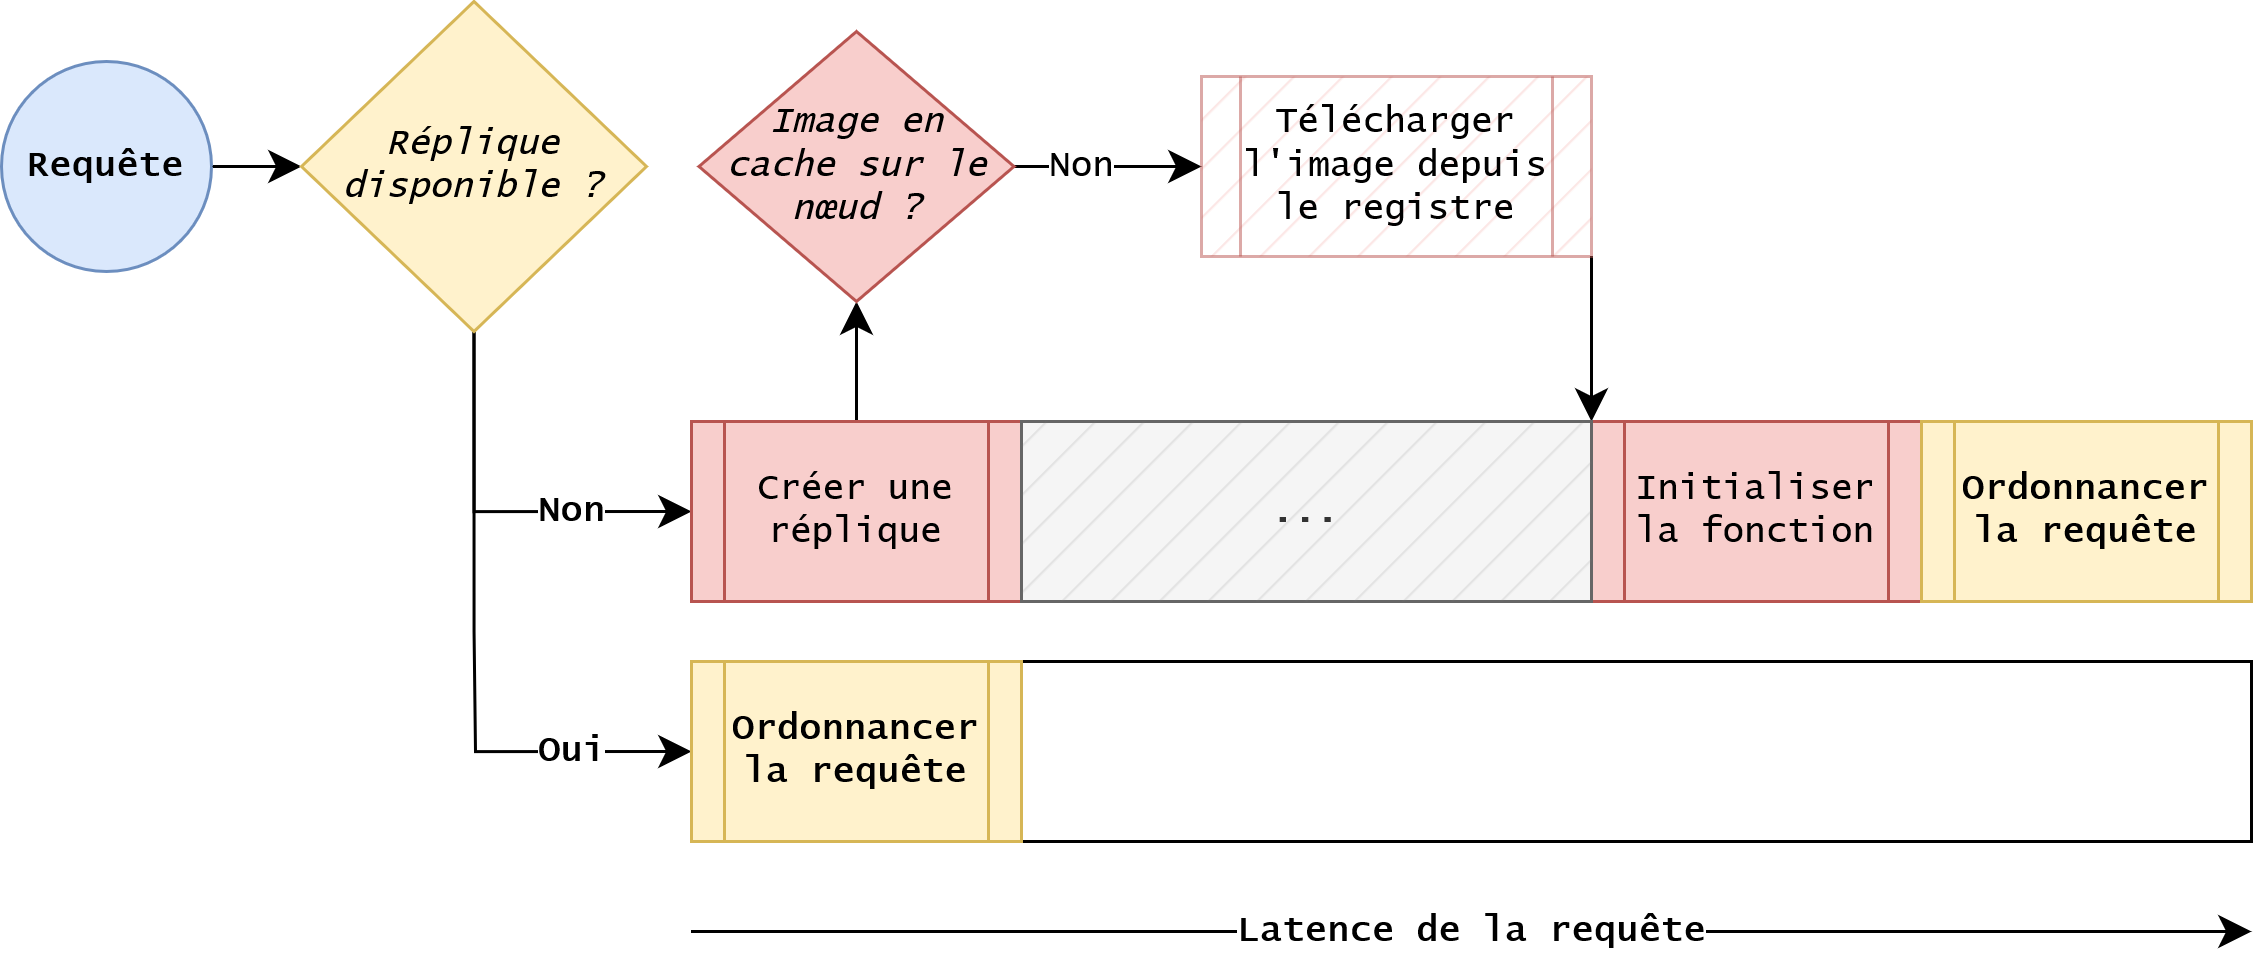
\includegraphics[width=0.8\columnwidth]{5_Chapitre5/figures/function-cache.png}
    \caption{Cycle de vie d'une requête utilisateur dans une plateforme serverless. L'arrivée d'une requête dans le système provoque des décisions de mise à l'échelle (en rouge) et d'ordonnancement (en jaune).}
    \label{figure:herocache-function-cache}
\end{figure}

Afin de répondre aux requêtes des utilisateurs sans dégrader les performances, l'autoscaler ajuste périodiquement le nombre de répliques pour chaque fonction déployée : le nombre de répliques croît et décroît en fonction des variations sur la charge des fonctions d'une application. Lorsque la charge sur une fonction augmente au-delà du seuil de concurrence de la plateforme, l'autoscaler crée une nouvelle réplique qui traitera les requêtes supplémentaires des utilisateurs. Lorsque la charge diminue, les répliques inactives sont supprimées. S'il n'y a plus de requêtes pour une fonction donnée, celle-ci peut être \textit{mise à l'échelle jusqu'à zéro}, ce qui permet de réattribuer des ressources matérielles à des tâches plus pressantes. Les répliques de cette fonction peuvent alors être détruites. Lorsqu'une fonction est demandée alors qu'aucune réplique n'existe, elle passe par un \textbf{démarrage à froid} qui entraîne un délai d'initialisation qui s'ajoute au temps de réponse de la fonction.

Ce démarrage à froid présente un risque d'augmentation du temps de réponse d'une application, car la plateforme doit allouer des ressources matérielles pour instancier chacune des fonctions qui la composent avant de répondre à la requête. Plus l'application est complexe, plus le risque de retards cumulés est élevé~\cite{mohanAgileColdStartsa}.

Les répliques de fonctions sont initialisées à partir d'\textbf{images de fonctions} (\textit{e.g.} une image Docker ou de machine virtuelle). Celles-ci sont stockées dans un registre d'images. Ces registres peuvent être accessibles à distance par Internet, ou déployés dans l'infrastructure du fournisseur. Toutefois, de nombreuses études antérieures~\cite{bhasiCypressInputSizesensitive2022, zijunFassflowEfficient2022, smithFaDOFaaSFunctions2022, zhangFIRSTExploitingMultiDimensional2023} n'envisagent que des scénarios favorables, dans lesquels les images de fonctions sont déjà disponibles sur les nœuds edge. Cela ne reflète pas la réalité, puisque les images de fonctions sont stockées dans des registres, sur des nœuds dédiés, et téléchargées sur les nœuds edge lors du déploiement des fonctions (figure~\ref{figure:herocache-function-cache}). En fonction de la taille de l'image, cela peut avoir des conséquences négatives sur la latence des requêtes avec des déploiements où les démarrages à froid dominent le temps de réponse total d'une fonction~\cite{yanHermesEfficientCache2020}.

Ce processus d'initialisation des répliques à partir d'images sur les nœuds edge peut représenter jusqu'à 80\% du temps de réponse d'une fonction~\cite{yanHermesEfficientCache2020} dans les cas où la latence introduite par le démarrage à froid domine le temps de réponse total de la fonction. Cette situation n'est pas acceptable lorsque la plateforme doit répondre à des exigences strictes en matière de qualité de service, comme c'est le cas pour les tâches critiques telles que l'\gls{IDS}.

\subsection{Communications entre les fonctions}
\label{section:herocache-background-communications}

\begin{figure}[!ht]
    \centering
    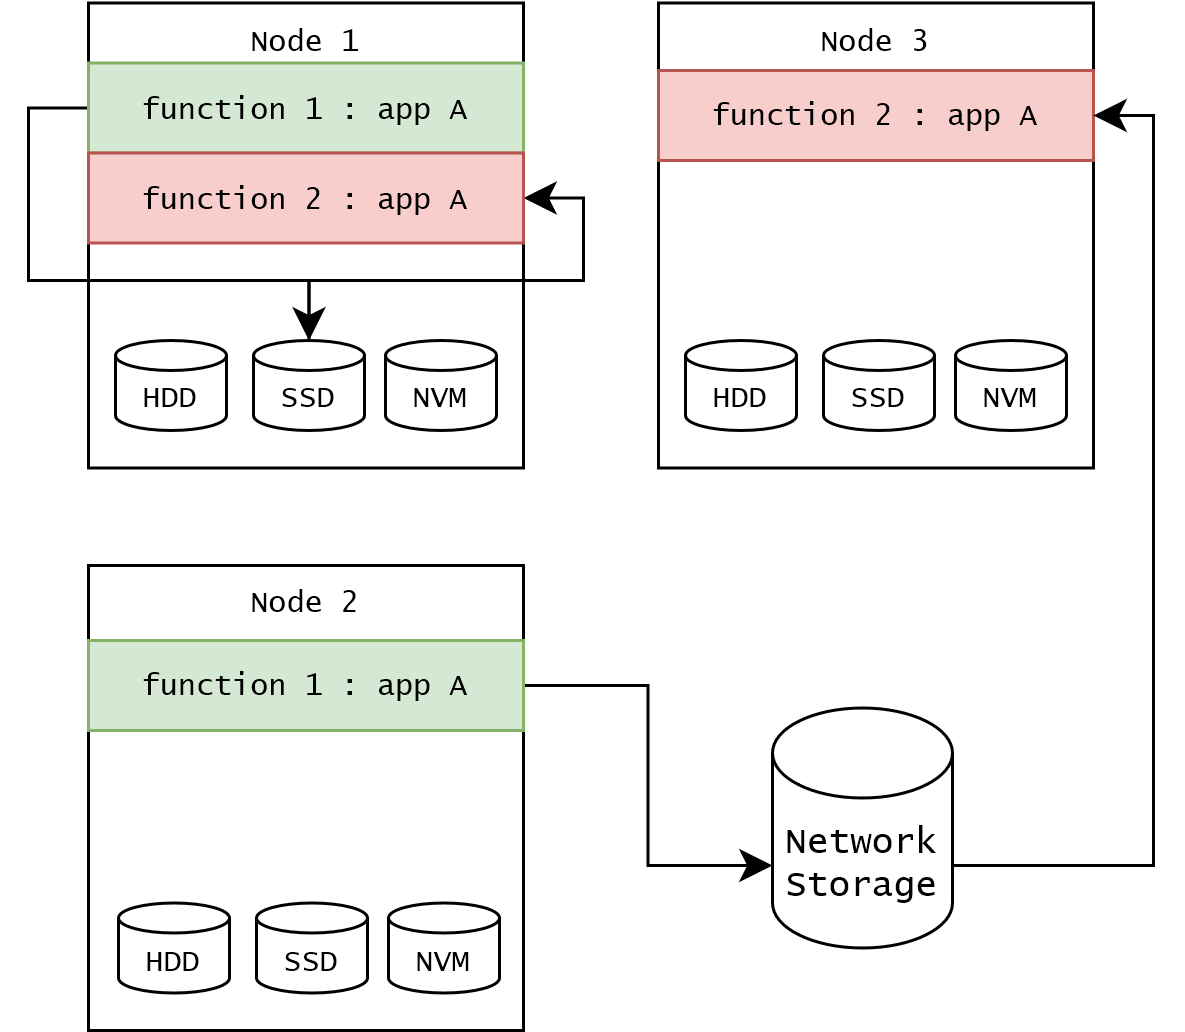
\includegraphics[width=0.8\columnwidth]{5_Chapitre5/figures/function-communications.png}
    \caption{Les fonctions serverless communiquent des résultats intermédiaires à travers un stockage persistant, qui peut être local aux nœuds et rapide (cas du premier nœud de la figure), ou accédé par le réseau et lent (cas des nœuds 2 et 3).}
    \label{figure:herocache-function-communications}
\end{figure}

Pour rendre possible la mise à l'échelle dynamique des fonctions, il est nécessaire que chaque invocation d'une fonction serverless soit indépendante, c'est-à-dire qu'elle ne porte pas les données ou le contexte des invocations précédentes. Cela permet aux répliques de mettre en file d'attente les requêtes utilisateur et de les traiter de manière séquentielle sans avoir besoin de procéder à un démarrage à froid entre les requêtes. Cela introduit une contrainte sur la plateforme serverless : si une application est composée de plusieurs fonctions qui forment une chaîne de traitement, la sortie de chaque fonction doit être sauvegardée dans un stockage persistant pour être passée en entrée de la fonction suivante dans la chaîne~\cite{mullerLambadaInteractiveData2020} (figure~\ref{figure:herocache-function-communications}).

Les travaux de l'état de l'art ont montré que les fonctions serverless qui communiquent, \textit{via} le réseau, par le biais d'un stockage distant, peuvent subir un ralentissement jusqu'à 11x supérieur par rapport aux fonctions utilisant des communications directes~\cite{wawrzoniakBoxerDataAnalytics2021a} (\textit{e.g.} au travers de mémoire partagée au sein d'un même nœud). Les fonctions de notre application d'\gls{IDS} doivent communiquer des résultats intermédiaires à chaque étape du DAG de l'application. Lorsque les fonctions sont déployées sur différents nœuds edge, les communications inter-fonctions devront être réalisées par l'utilisation d'un stockage à distance. Cela introduit des ralentissements qui peuvent faire boule de neige tout au long de l'exécution des fonctions et détériorer la qualité de service de l'ensemble de l'application.

\section{Proposition d'une plateforme pour la détection d'intrusion à l'edge dans le modèle serverless}
\label{section:herocache-before-contrib}

\begin{figure*}[!ht]
    \centering
    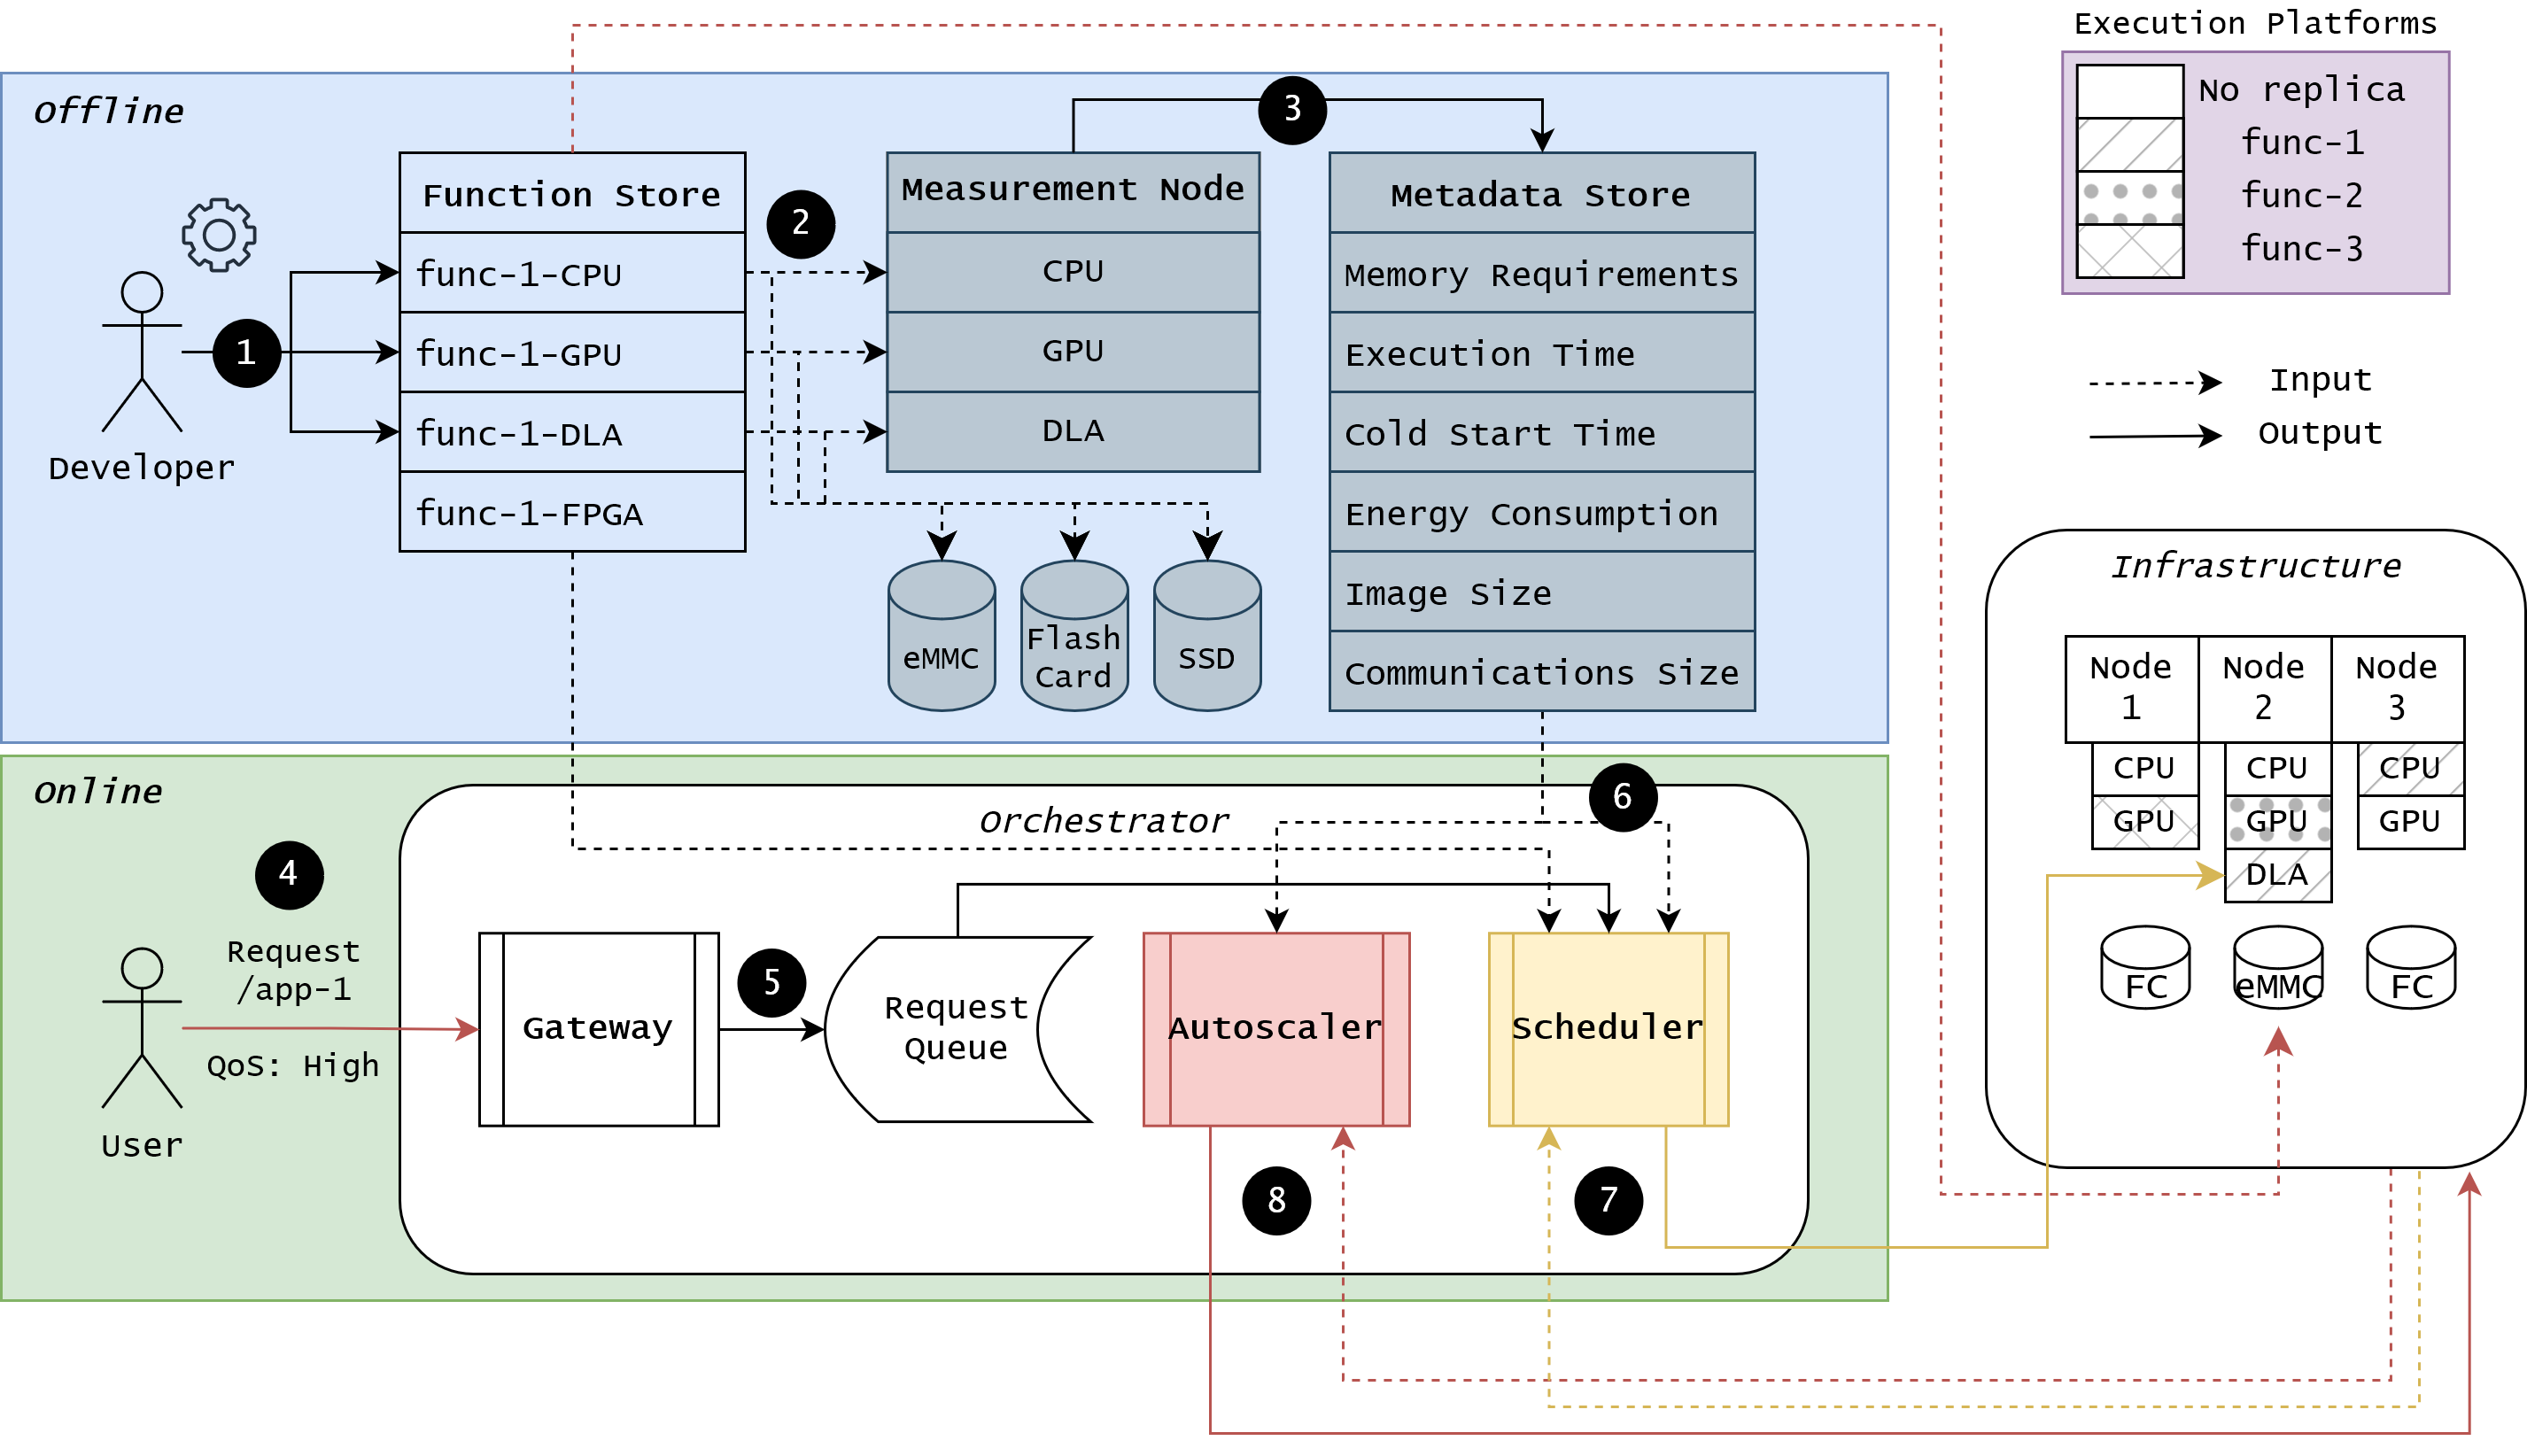
\includegraphics[width=0.8\textwidth]{5_Chapitre5/figures/serverless-platform-storage.png}
    \caption{Plateforme serverless pour le déploiement d'une application d'\gls{IDS}.}
    \label{figure:herocache-serverless-platform}
\end{figure*}

Orchestrer des applications tout en respectant les accords de niveau de service (\gls{SLA}, pour \textit{Service Level Agreement}) nécessite de modéliser précisément les caractéristiques de l'application et d'en tenir compte lors de l'allocation des ressources et de l'ordonnancement des requêtes utilisateur sur la plateforme serverless. La figure~\ref{figure:herocache-serverless-platform} donne un aperçu du cycle de vie d'une application sur notre plateforme. Il est divisé en deux phases ; une \textbf{phase hors-ligne} qui consiste à caractériser les applications déployées par les développeurs sur les plateformes edge, et une \textbf{phase en ligne} où les requêtes des utilisateurs vers ces applications sont ordonnancées sur la plateforme.

\textbf{Phase hors-ligne}. Dans notre plateforme, le cycle de vie de l'application commence par une phase hors-ligne, au cours de laquelle le développeur fournit le code de ses fonctions pour différentes architectures matérielles (\gls{GPU}, \gls{CPU}, \gls{DLA}, etc.)~\Circled{1}. Ce code est stocké par le fournisseur de services dans un registre de fonctions. Les fonctions sont ensuite déployées sur un nœud de mesure~\Circled{2} où elles sont exécutées afin de produire des métadonnées relatives à leur exécution sur des nœuds hétérogènes. Les besoins en mémoire, le temps d'exécution, le temps de démarrage à froid, la consommation d'énergie, la taille de la fonction et la taille des données communiquées pour chaque fonction sont enregistrés dans un registre de métadonnées~\Circled{3}. L'exécution de la phase hors-ligne est nécessaire une fois pour une fonction donnée sur une plateforme donnée, comme décrit dans la section~\ref{section:herocache-workload}.

\textbf{Phase en ligne}. Les requêtes utilisateur envoyées aux applications d'\gls{IDS} comportent un extrait de trafic réseau (sous forme de paquets \gls{TCP}, pour \textit{Transmission Control Protocol}, sérialisés) à analyser~\Circled{4}, et sont associées à un niveau de qualité de service souhaité pour le temps de réponse de la requête. La requête est ajoutée à une file d'attente~\Circled{5} au niveau de l'orchestrateur. Lorsque l'ordonnanceur extrait la requête de la file d'attente, il interroge le registre pour récupérer les métadonnées de fonction appropriées~\Circled{6}.

L'ordonnanceur tente alors de trouver une réplique disponible de la première fonction de l'application pour traiter la requête~\Circled{7}. Si une telle réplique n'existe pas encore, il sera demandé à l'autoscaler d'initialiser une nouvelle instance de la fonction~\Circled{8}. Au cours du cycle de vie de l'application, l'autoscaler vérifie périodiquement la charge moyenne de chaque fonction pour ajuster le nombre de répliques déployées sur la plateforme, en fonction du seuil de concurrence fixé par le fournisseur de services.

Lorsque l'application termine son exécution, elle retourne à l'utilisateur un vecteur de classification qui indique les probabilités que le trafic soit malveillant, c'est-à-dire qu'il présente les caractéristiques d'une attaque potentielle.

\section{Phase hors-ligne : caractérisation} 
\label{section:herocache-workload}

Dans cette section, nous détaillons notre méthodologie et donnons les résultats de la campagne de mesures menée dans le but de caractériser les plateformes d'exécution ainsi que les tâches considérées dans cette contribution.

Ces travaux ont été menés conjointement avec Camélia Slimani, co-autrice de la publication associée à ce chapitre~\cite{herocache}.

\begin{figure}[!ht]
    \centering
    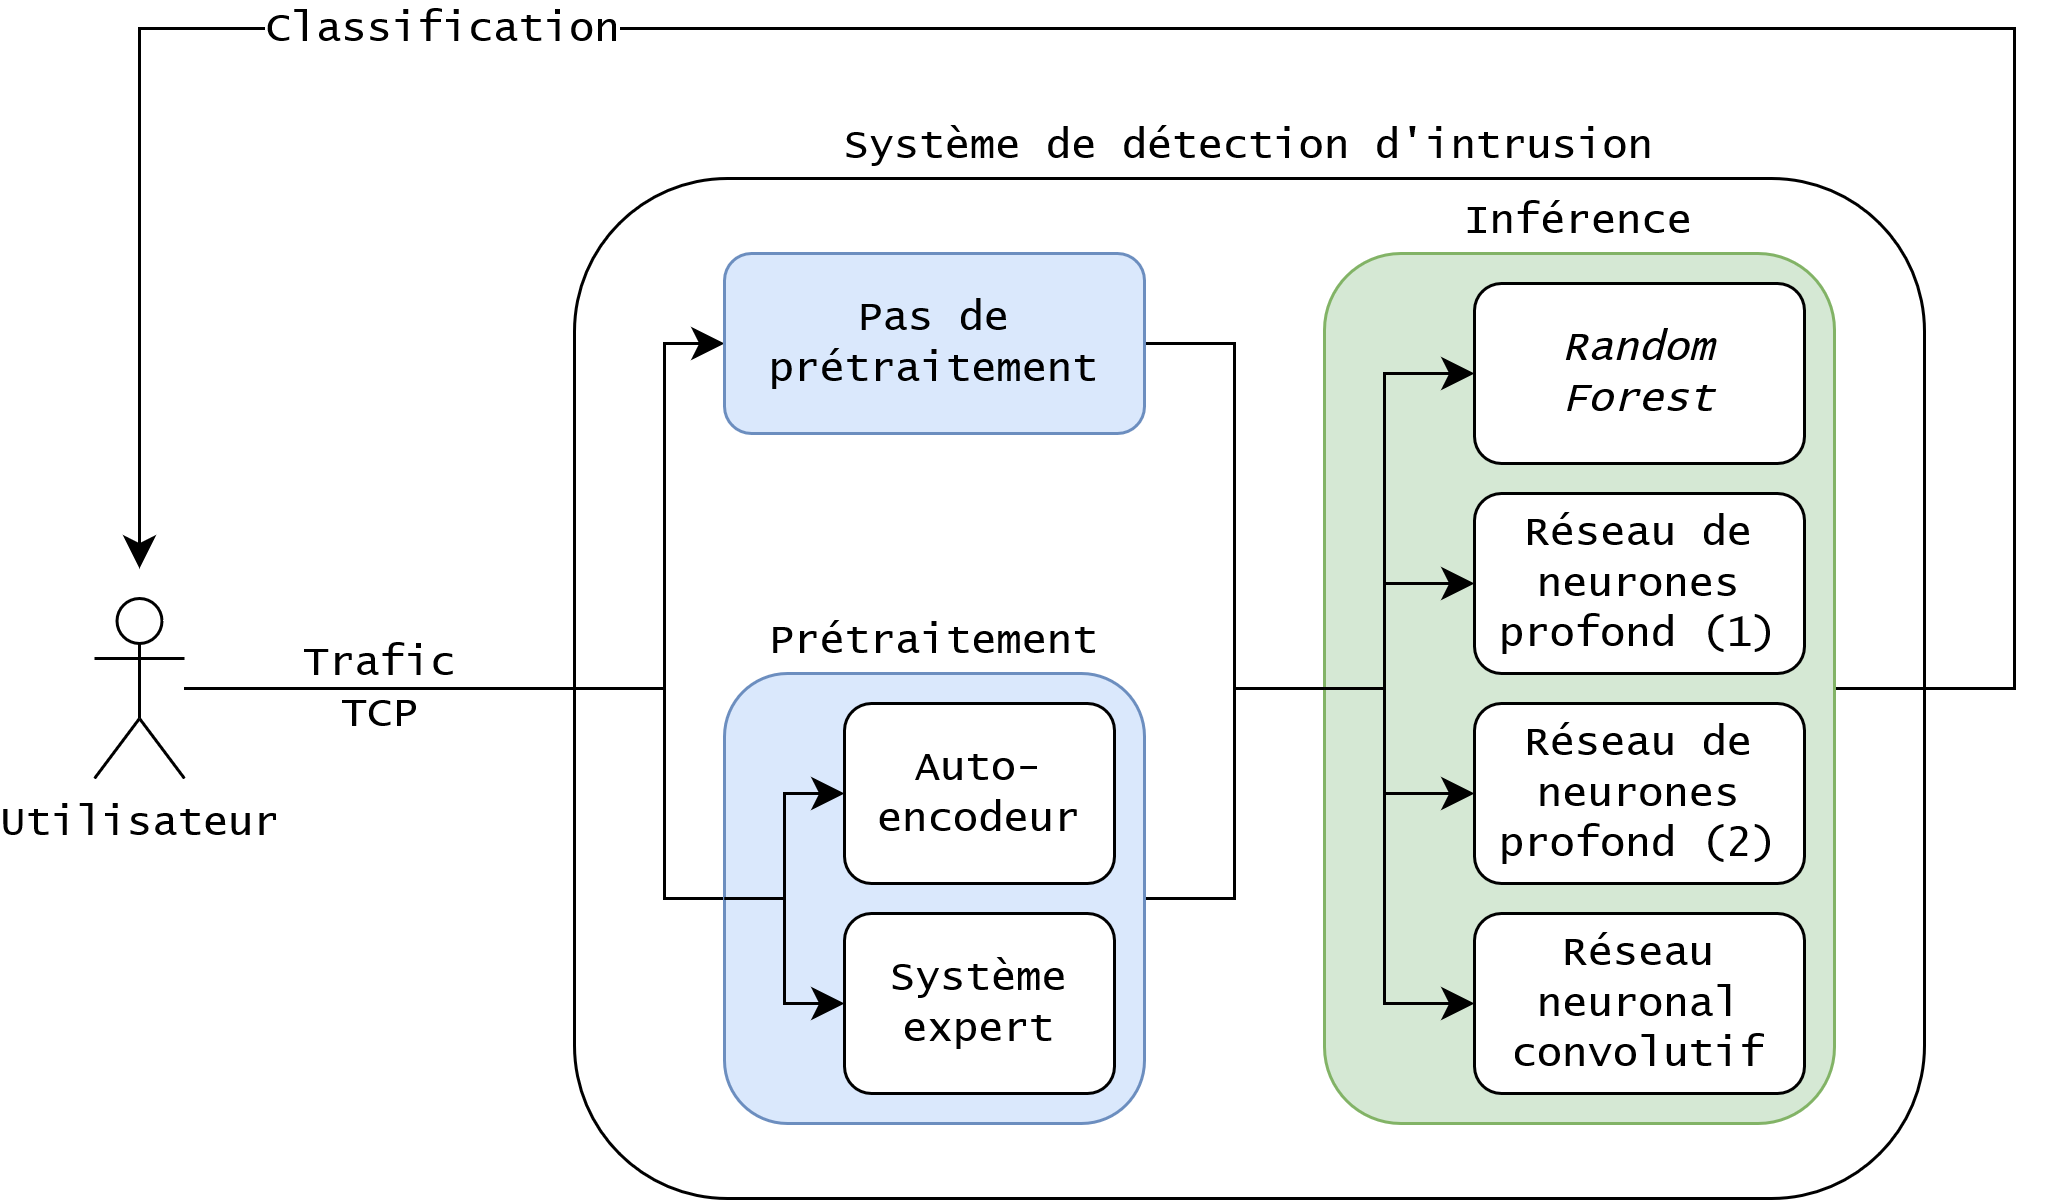
\includegraphics[width=0.8\columnwidth]{5_Chapitre5/figures/ids-application.png}
    \caption{Architecture de l'application d'\gls{IDS} considérée. Elle peut éventuellement exploiter différentes fonctions de prétraitement, et différentes fonctions d'inférence pour fournir une classification du trafic \gls{TCP} à l'utilisateur.}
    \label{figure:herocache-ids-application}
\end{figure}

Pour parvenir à une allocation des ressources et à un placement des tâches adéquats lors de l'exécution des applications d'\gls{IDS}, il est nécessaire de caractériser les plateformes d'exécution ainsi que les fonctions logicielles qui seront mobilisées~\cite{mampageHolisticViewResource2022}. À cette fin, nous avons évalué plusieurs modèles de détection d'intrusion en termes de performance et de consommation d'énergie sur des plateformes hétérogènes représentatives de dispositifs edge~\cite{kljucaric2020}. Cette section décrit notre méthodologie et nos résultats.

\subsection{Caractérisation des plateformes d'exécution} \label{section:herocache-characterization-platforms}

Nous avons utilisé des plateformes représentatives de ce que l'on peut trouver à l'edge~\cite{slimani:hal-04159551, kljucaric2020} :
\textbf{(1) Raspberry Pi 4B}, équipée d'un \gls{CPU} quadricœur ARM Cortex-A72, de 4 GB LPDDR4 en mémoire principale et d'une carte SD de 16 GB. La carte fonctionne sous Linux 5.4, avec la distribution Raspbian.
\textbf{(2) Nvidia Jetson Xavier AGX}, composée de trois éléments de traitement : un \gls{CPU} NVIDIA ARM Carmel à 8 cœurs, un \gls{GPU} NVIDIA Volta avec 512 cœurs CUDA et un accélérateur d'apprentissage profond (\gls{DLA}, pour \textit{Deep Learning Accelerator}), qui est un accélérateur matériel à fonction fixe conçu pour les réseaux neuronaux convolutifs (\gls{CNN}, pour \textit{Convolutional Neural Network}). Il est supposé être plus économe en énergie que le \gls{GPU}. La carte Xavier AGX est équipée de 16 GB de mémoire LPDDR4 et de 32 GB de mémoire flash eMMC 5.1. Elle fonctionne sous Linux Tegra 4.9.10. Le mode d'alimentation \textit{15 Watts Desktop} a été utilisé.
\textbf{(3) PYNQ-Z2 Development Board}, une carte basée sur le système sur puce (\gls{SoC}, pour \textit{System on Chip}) Xilinx Zynq XC7Z020. Elle est équipée d'un \gls{FPGA} Artix-7, d'une mémoire DDR3 de 512 MB et d'une carte SD de 16 GB.

\subsection{Caractérisation des applications}
\label{section:herocache-characterization-workloads}

Notre application, schématisée en figure~\ref{figure:herocache-ids-application}, se compose de différents préprocesseurs et classifieurs. Le préprocesseur sélectionne un sous-ensemble de caractéristiques pertinentes des paquets \gls{TCP} fournis par l'utilisateur. Trois approches de prétraitement différentes ont été retenues : (1) utilisation de toutes les caractéristiques des paquets sans aucune sélection (\textit{NoFS}, pour \textit{No Feature Selection}) ; (2) utilisation d'un auto-encodeur {\gls{DNN} (pour \textit{Deep Neural Network}) pour projeter les caractéristiques dans un espace latent plus petit (\gls{AE}, pour \textit{Autoencoder}) ; et (3) sélection experte d'un sous-ensemble de caractéristiques (\gls{ES}, pour \textit{Expert Selection}). Pour la partie classification, nous avons utilisé un algorithme de \textit{Random Forest} (\gls{RF}), deux architectures différentes de réseaux neuronaux denses (\gls{DNN}) et un \gls{CNN}.

\begin{table}[t]
\caption{Architecture et taille des modèles d'\gls{IDS} considérés.}
\resizebox{\textwidth}{!}{
\begin{tabular}{|c|c|cc|}
\hline
Modèle     & Architecture                                                                                                                                         & \multicolumn{1}{c|}{Taille du modèle sur \gls{CPU} (Mo)} & Taille du modèle sur \gls{GPU} (Mo) \\ \hline
NoFS-RF   & \begin{tabular}[c]{@{}c@{}}5 arbres de \\ profondeur maximale 100 \end{tabular}                                                                               & \multicolumn{1}{c|}{28}                      & 15,4                   \\ \hline
AE-RF     & \begin{tabular}[c]{@{}c@{}}5 arbres de \\ profondeur maximale 50 \end{tabular}                                                                               & \multicolumn{1}{c|}{-}                       & 32,9                   \\ \hline
ES-RF     & \begin{tabular}[c]{@{}c@{}}10 arbres de \\ profondeur maximale 10 \end{tabular}                                                                              & \multicolumn{1}{c|}{9,1}                     & 5,5                    \\ \hline
NoFS-DNN1 & \multirow{3}{*}{\begin{tabular}[c]{@{}c@{}}4 couches denses \\ (128x64x32x10)\end{tabular}}                                                            & \multicolumn{2}{c|}{0,144}                                            \\ \cline{1-1} \cline{3-4} 
AE-DNN1   &                                                                                                                                                      & \multicolumn{2}{c|}{0,321}                                            \\ \cline{1-1} \cline{3-4} 
ES-DNN1   &                                                                                                                                                      & \multicolumn{2}{c|}{0,053}                                            \\ \hline
NoFS-DNN2 & \multirow{3}{*}{\begin{tabular}[c]{@{}c@{}}5 couches denses \\ (7024x704x288x64x10)\end{tabular}}                                                      & \multicolumn{2}{c|}{3,33}                                             \\ \cline{1-1} \cline{3-4} 
AE-DNN2   &                                                                                                                                                      & \multicolumn{2}{c|}{2,96}                                             \\ \cline{1-1} \cline{3-4} 
ES-DNN2   &                                                                                                                                                      & \multicolumn{2}{c|}{2,61}                                             \\ \hline
NoFS-CNN  & \multirow{3}{*}{\begin{tabular}[c]{@{}c@{}}2 Conv1D (x64) - MaxPool \\ 3 Conv1D (x256) - MaxPool\\ 3 couches denses (100x20x10)\end{tabular}} & \multicolumn{2}{c|}{4,77}                                             \\ \cline{1-1} \cline{3-4} 
AE-CNN    &                                                                                                                                                      & \multicolumn{2}{c|}{2,9}                                              \\ \cline{1-1} \cline{3-4} 
ES-CNN    &                                                                                                                                                      & \multicolumn{2}{c|}{2,6}                                              \\ \hline
\end{tabular}
}
\label{table:herocache-workload}
\end{table}

Le tableau~\ref{table:herocache-workload} présente les modèles d'\gls{IDS} pris en compte dans cette étude et certaines de leurs caractéristiques. Ces modèles ont été entraînés et caractérisés sur un jeu de données de l'état de l'art représentant des intrusions sur le réseau, UNSW-NB15\footnote{\href{https://research.unsw.edu.au/projects/unsw-nb15-dataset}{https://research.unsw.edu.au/projects/unsw-nb15-dataset}}. Dans ce jeu de données, chaque observation représente des caractéristiques statistiques, de contenu et de temps sur le trafic au cours d'une fenêtre temporelle, et est étiquetée comme "normale" ou "attaque". Le jeu de données comprend neuf catégories d'attaques. Les modèles de réseaux neuronaux ont été exportés et optimisés à l'aide de TensorFlow Lite et TensorRT lorsqu'ils étaient destinés à des plateformes \gls{CPU} et \gls{GPU}/\gls{DLA}, respectivement. En ce qui concerne Random Forest, les modèles ont été exportés en utilisant les frameworks Emlearn et HummingBird.ml lorsqu'ils étaient destinés aux plateformes \gls{CPU} et \gls{GPU}, respectivement. hls4ml a été utilisé pour exporter les modèles de réseaux neuronaux pour la cible \gls{FPGA} par un procédé de synthèse de haut niveau (\textit{HLS}, pour \textit{High-Level Synthesis}), qui transforme le code source C++ en une représentation intermédiaire (\gls{RTL}, pour \textit{Register Transfer Level}) adaptée à la cible.

\subsection{Mesures de performances}

Pour mesurer leur latence lors de l'inférence, chacun des modèles d'\gls{IDS} a été déployé sur les plateformes cibles pour être évalué sur un ensemble de $80 000$ paquets provenant du jeu de données \textit{UNSW-NB15}. Les résultats sont présentés dans la figure~\ref{figure:herocache-performance}. Seul un modèle (ES-DNN1) a été caractérisé sur la plateforme \gls{FPGA} car les représentations RTL des autres modèles après synthèse n'ont pas pu être acceptées par la cible. La conclusion qui a été tirée de ces résultats est que pour les réseaux neuronaux, le \gls{CPU} Xavier atteint la meilleure performance dans la majorité des cas, à l'exception de NoFS-CNN qui profite des capacités du \gls{GPU} en raison de son nombre élevé de paramètres et de l'efficacité du \gls{GPU} pour les opérations de convolution. Pour les modèles Random Forest, l'élément de traitement le plus rapide est le \gls{GPU}. En termes de coût et de disponibilité, la Xavier AGX est respectivement environ 20x et 10x plus chère que les plateformes RBPI4 et Pynq-Z2. Nous dimensionnons notre infrastructure en conséquence, en intégrant plus de plateformes RBPI4 que de Xavier AGX pour être représentatifs de déploiements réels.

\begin{figure}
    \centering
    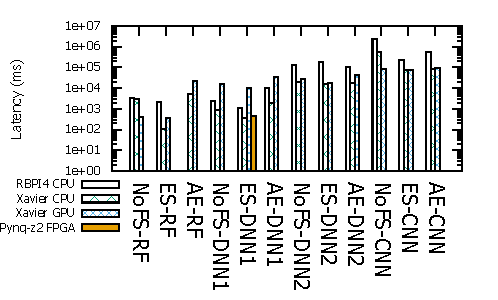
\includegraphics[width=0.6\columnwidth]{5_Chapitre5/figures/latency_bar.pdf}
    \caption{Mesures de la latence des modèles d'\gls{IDS} considérés.}
    \label{figure:herocache-performance}
\end{figure}

\subsection{Mesures de consommation d'énergie}

Nous avons exécuté des inférences sur les modèles d'\gls{IDS} sur chaque élément de traitement et mesuré la consommation d'énergie de la plateforme à l'aide de l'analyseur de puissance N6705A DC. Les résultats sont présentés dans la figure~\ref{figure:herocache-energy}. Pour les mêmes raisons que mentionné ci-dessus, seul ES-DNN1 a été caractérisé sur \gls{FPGA}. Nous observons que les plateformes \gls{CPU} affichent une consommation d'énergie inférieure à celle du \gls{GPU} dans la majorité des cas~\cite{slimani:hal-04159551, SLIMANI2024}. Le seul cas où le \gls{GPU} obtient de meilleurs résultats est lorsque la vitesse qu'il atteint par rapport aux \gls{CPU} est élevée. C'est par exemple le cas pour NoFS-CNN, où le \gls{CPU} RBPI4 est plus de 30 fois plus lent que le \gls{GPU}. Même si la carte Pynq-Z2 présente la meilleure efficacité énergétique avec le modèle ES-DNN1, étant donné qu'elle est plus chère et présente une généricité limitée en matière de conception, nous supposons qu'elle est moins disponible que le RBPI4.

\begin{figure}
    \centering
    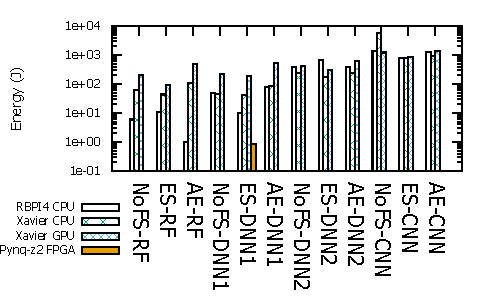
\includegraphics[width=0.6\columnwidth]{5_Chapitre5/figures/energy_bar.pdf}
    \caption{Mesures de la consommation d'énergie des modèles d'\gls{IDS} considérés.}
    \label{figure:herocache-energy}
\end{figure}

\section{Phase en ligne : orchestration avec HeROcache} \label{section:herocache-contribution}

Dans cette section, nous formulons le problème que notre contribution cible, puis nous donnons une description détaillée de notre modèle. Enfin, nous présentons une description formelle de notre stratégie pour la mise à l'échelle automatique des ressources et l'ordonnancement des tâches.

\subsection{Présentation générale}

L'orchestrateur HeROcache est principalement composé de deux modules, un \textbf{autoscaler} et un \textbf{ordonnanceur} (voir figure~\ref{figure:herocache-serverless-platform}). L'autoscaler est chargé de l'allocation dynamique des ressources : il affecte les plateformes d'exécution aux répliques de fonctions. L'ordonnanceur s'occupe du placement des requêtes utilisateur sur les répliques.

HeROcache relève les trois défis susmentionnés en proposant des stratégies complémentaires de minimisation des coûts au niveau de l'autoscaler et de l'ordonnanceur. HeROcache minimise \textbf{les délais d'initialisation} en tenant compte des temps de latence induits par la récupération des images de fonctions au niveau de l'autoscaler. Une stratégie de \textit{prefetching} (ou \textit{préchargement}) est également mise en œuvre, qui consiste à essayer de mettre en cache des images de fonctions pertinentes en avance de phase. Les coûts de \textbf{communications inter-fonction} sont pris en compte principalement dans l'ordonnanceur, qui tend naturellement à consolider les fonctions d'une même application. L'autoscaler participe indirectement à cette consolidation par le \textit{prefetching}, en mettant en cache les fonctions suivantes du DAG de l'application sur le même nœud. Enfin, l'\textbf{hétérogénéité matérielle} est prise en compte car les différents facteurs de coût d'exécution extraits pendant la phase hors-ligne (voir section~\ref{section:herocache-workload}) sont exploités tout au long du processus d'autoscaling et d'ordonnancement. Les sections suivantes décrivent les stratégies de mise à l'échelle automatique et d'ordonnancement.

\subsection{Stratégie de minimisation des coûts d'allocation des ressources}

\begin{table}[!ht]
    \caption{Dictionnaire des notations.}
    \begin{center}
    \scalebox{0.85}{
        \begin{tabularx}{\linewidth}{|c|Z|}
            \hline \textbf{Notation} & \textbf{Description} \\ \hline
            $x_a$ & Allocation des ressources pour une application $a$ \\ \hline
            $y_a$ & Invocation d'une application $a$ \\ \hline
            $z_i$ & Placement d'une tâche pour la fonction $i$ \\ \hline
            $f_{N, P}$ & Une fonction $f$ déployée pour exécution sur une plateforme $P$ disponible sur un nœud $N$ \\ \hline
            $f_{a}$ & Une fonction $f$ appartenant à une application $a$ \\ \hline
            $A$ & Nombre total d'applications disponibles pour déploiement sur la plateforme \\ \hline
            $F_{a}$ & Nombre total de fonctions appartenant à une application $a$ \\ \hline
            $RT_{{f}_{N, P}}$ & Temps de récupération de l'image de la fonction $f$ pour un déploiement sur une plateforme $P$ disponible sur un nœud $N$ \\ \hline
            $NB_{N}$ & Bande passante réseau disponible entre un nœud $N$ et l'infrastructure \\ \hline
            $SMT_{N}$ & Débit du support de stockage disponible sur un nœud $N$ \\ \hline
            $SML_{N}$ & Latence du support de stockage disponible sur un nœud $N$ \\ \hline
            $QP$ & Pénalité sur violation de qualité de service \\ \hline
            $QD$ & Facteur de ralentissement par niveau de qualité de service \\ \hline
            $WCET$ & Pire temps d'exécution \\ \hline
            $TT$ & Temps total pour une tâche \\ \hline
            $CST$ & Temps de démarrage à froid \\ \hline
            $ST$ & Temps des opérations de stockage \\ \hline
            $ET$ & Temps d'exécution nominal d'une fonction \\ \hline
            $EC$ & Consommation d'énergie \\ \hline
            $IS$ & Taille de l'image d'une fonction \\ \hline
            $HP$ & Prix du matériel \\ \hline
            $TC$ & Consolidation des tâches \\ \hline
            $Q$ & File d'attente des requêtes dans une réplique \\ \hline
            $CP$ & Proportion de fonctions mises en cache sur un nœud pour une application donnée \\ \hline
            $SIS^{f}_{a}$, $SOS^{f}_{a}$ & Respectivement les tailles des données d'entrée et de sortie d'une fonction $f$ appartenant à une application $a$ \\ \hline
            $threshold_{f, h}$ & Seuil de concurrence pour une fonction $f$ sur un type de matériel $h$ \\ \hline
            $scaleCost^{{f}_{{i}_{N, P}}}_a$ & Coût de la création d'une nouvelle réplique pour une fonction $f_i$ d'une application $a$ sur une plateforme $P$ disponible sur un nœud $N$ \\ \hline
            $schedCost^{{f}_{{i}_{N, P}}}_a$ & Coût de l'ordonnancement d'une tâche pour une fonction $f_i$ d'une application $a$ sur une plateforme $P$ disponible sur un nœud $N$ \\ \hline
        \end{tabularx}
    }
    \label{table:herocache-notation}
    \end{center}
\end{table}

Nous formulons l'allocation des ressources comme un problème d'optimisation et nous le résolvons à l'aide d'un algorithme glouton simple. L'objectif de l'autoscaler est de minimiser la somme des coûts des allocations $scaleCost_{a}$ pour $y_a$ invocations de l'application $a$ (équation~\ref{eq:herocache-objective-allocation}), pour toutes les applications dans $A$, sous contrainte d'une infrastructure finie avec $x_a$ l'allocation de ressources pour l'application $a$ (équation~\ref{eq:herocache-constraint-allocation}).

\begin{equation}
    \forall A, \, \min \sum_{a = 0}^{A} y_a \cdot scaleCost_{a}
\label{eq:herocache-objective-allocation}
\end{equation}

\begin{equation}
    \text{s. t.} \, \sum_{a = 0}^{A} x_a \leq Total Resources
\label{eq:herocache-constraint-allocation}
\end{equation}

Le coût de l'allocation des ressources pour une application $a$ est la somme des coûts d'allocation pour les fonctions qui la composent (équation~\ref{eq:herocache-scale-cost-app}). Une réplique est allouée à une plateforme d'exécution.

\begin{equation}
    scaleCost_{a} = \, \sum_{i = 0}^{F_{a}} scaleCost^{{f}_{{i}_{N, P}}}_a
\label{eq:herocache-scale-cost-app}
\end{equation}

Chaque réplique de fonction a un coût d'allocation associé, car l'allocation dynamique des ressources matérielles introduit un temps de latence lors du traitement des requêtes utilisateur.

Nous avons conçu un modèle de coût (équation~\ref{eq:herocache-scale-cost-function}) pour l'allocation des ressources nécessaires au déploiement d'une fonction d'une application donnée. Il est composé de quatre éléments, dont nous devons minimiser la somme :

\begin{itemize}
    \item La \textit{proportion de cache} $CP$ traduit la dispersion des fonctions sur les différents nœuds edge. Plus le score est élevé, plus les fonctions sont dispersées sur les nœuds. La minimisation de ce terme permet de consolider les fonctions ;
    \item Le \textit{temps total} $TT$ représente le temps d'exécution total de la fonction. Il tient compte de la qualité de service de l'application, de l'hétérogénéité de la plateforme et du coût de déploiement (si l'image est mise en cache sur le nœud ou distante). Plus ce coût est élevé, plus la qualité de service est faible ;
    \item La \textit{consommation d'énergie} $EC$ traduit la consommation d'énergie du déploiement de la fonction. Plus $EC$ est élevé, plus le coût est important ;
    \item Le \textit{prix du matériel} $HP$ décrit le coût total de possession (\textit{TCO}, pour \textit{Total Cost of Ownership}) supporté par les fournisseurs de services en fonction du temps d'exécution. Il traduit le coût de déploiement sur une plateforme matérielle donnée. Plus $HP$ est élevé, plus le coût de la solution est important.
\end{itemize}

L'objectif global du modèle de coût est de déployer une fonction au coût le plus bas possible, c'est-à-dire avec une consolidation accrue, une réduction du \textit{makespan} (le temps total d'exécution), une réduction de la consommation d'énergie et une réduction du coût de possession. Nous détaillerons chaque partie de l'équation~\ref{eq:herocache-scale-cost-function} dans les paragraphes suivants. Chaque composante de l'équation est pondérée pour permettre un réglage souple ; les valeurs que nous avons choisies pour le déploiement de l'application d'\gls{IDS} sont spécifiées dans la partie consacrée à l'évaluation (section~\ref{section:herocache-evaluation}).

\begin{equation}
    \begin{split}
     \forall N, \forall P \in N, scaleCost^{{f}_{{i}_{N, P}}}_{a} = \,   &k_{CP} \cdot {CP}_{{a}_{N}}    \\
        + &k_{TT} \cdot {TT}_{{f}_{N, P}} \\
        + &k_{EC} \cdot {EC}_{{f}_{N, P}} \\
        + &k_{HP} \cdot {HP}_{{f}_{N, P}}
    \end{split}
    \label{eq:herocache-scale-cost-function}
\end{equation}

\textbf{Consolidation des tâches}. Comme nous l'avons vu précédemment, la mise en œuvre de la consolidation des tâches (donc des exécutions de fonctions) au sein des applications devrait permettre de minimiser les délais de communication qui pourraient s'accumuler au sein des chaînes de fonctions. HeROcache favorise le déploiement de répliques d'une fonction sur des nœuds où d'autres fonctions appartenant à la même application sont déjà déployées.

Pour ce faire, HeROcache surveille pour chaque application $a$ la proportion d'images des fonctions ${f}_{i}$ qui la composent déjà disponibles en cache, c'est-à-dire sur le stockage local du nœud. Cette proportion est notée $CF_{a}^{{f}_{i_{N, P}}}$ et calculée pour un nœud $N$ donné, pour une plateforme d'exécution $P$ donnée (équation~\ref{eq:herocache-cached-functions}).

Cette proportion est calculée pour chaque application, puis la moyenne est calculée sur toutes les applications s'exécutant sur un nœud donné.

\begin{equation}
    \forall a \in A, \, \forall f \in a, \, CF_{a}^{{f}_{i_{N, P}}} = \frac{\sum_{i = 0}^{Fa} isCached(f_{i}, N, P)}{F_{a}}
\label{eq:herocache-cached-functions}
\end{equation}

En prenant l'inverse de la proportion de fonctions en cache sur chaque nœud pour une application donnée, on obtient une valeur élevée pour les applications peu consolidées (l'objectif étant de minimiser cette proportion), voir équation~\ref{eq:herocache-cache-proportion-app}.

\begin{equation}
    \forall N, \forall P \in N, \, {CP}_{{a}_{N}} = \, \frac{A}{\sum_{i = 0}^{F_{a}} CF_{a}^{{f}_{i_{N, P}}}}
\label{eq:herocache-cache-proportion-app}
\end{equation}

En plus de la minimisation des coûts, afin de réduire les délais de déploiement, l'autoscaler essaie de mettre en cache les images des chaînes de fonctions en avance de phase, lors du déploiement d'une nouvelle réplique sur un nœud. Il inspecte les chaînes de fonctions et télécharge séquentiellement les images de fonctions manquantes du registre distant vers le stockage local du nœud, de manière asynchrone. Cette technique permet de réduire la latence des requêtes futures~\cite{leeSPESOptimizingPerformanceResource2024a}.

\textbf{Temps total d'exécution}. La deuxième composante du coût de mise à l'échelle est le \textit{temps total d'exécution}. La minimisation du temps total d'exécution devrait empêcher les retards d'initialisation de faire boule de neige dans les chaînes de fonctions, évitant ainsi les violations des accords de niveau de service (\gls{SLA}).

Grâce aux métadonnées collectées sur chaque fonction pendant la phase hors-ligne, l'autoscaler est en mesure de prédire le temps total ${TT}_{{f}_{N, P}}$ de la première requête qui sera ordonnancée sur une nouvelle réplique de fonction (équation~\ref{eq:herocache-total-time-function}).

\begin{equation}
    {TT}_{{f}_{N, P}} = \, {RT}_{{f}_{N, P}} + {WT}_{{f}_{N, P}} + {CST}_{{f}_{N, P}} + {ET}_{{f}_{N, P}}
\label{eq:herocache-total-time-function}
\end{equation}

\begin{itemize}
    \item ${RT}_{{f}_{N, P}}$ est la durée de récupération de l'image de la fonction. Si l'image de la fonction est déjà mise en cache sur le nœud de calcul, cette durée est nulle ; sinon, elle dépend de la taille de l'image $IS$ et est influencée par la bande passante $NB$ du lien réseau, car l'image sera lue à partir d'un registre d'images distant, et par le débit du support de stockage du nœud $SMT$ ainsi que sa latence $SML$, car l'image sera écrite et stockée localement en vue d'une utilisation ultérieure (équation~\ref{eq:herocache-retrieval-time}) ;

    \begin{equation}
        {RT}_{{f}_{N, P}} = \, \frac{IS_{{f}_{N, P}}}{\min (NB_{N}, SMT_{N})} + SML_{N}
        \label{eq:herocache-retrieval-time}
    \end{equation}

    \item ${WT}_{{f}_{N, P}}$ est le temps que la tâche passera à attendre dans la file d'attente de la plateforme. Au moment de la création de la réplique, ce temps sera égal à zéro car nous ne prévoyons que la latence encourue par la première requête sur la réplique ;
    \item ${CST}_{{f}_{N, P}}$ est le temps de démarrage à froid nécessaire pour initialiser l'instance de la fonction (\textit{i.e.} décompresser l'image, préparer le conteneur, initialiser les bibliothèques, etc.). Il est mesuré en fonction des métadonnées extraites lors de la phase hors-ligne ;
    \item ${ET}_{{f}_{N, P}}$ est la durée d'exécution de la fonction, y compris le temps de communication avec ses prédécesseurs et successeurs potentiels dans le DAG. Cette durée tient compte des métadonnées extraites pour la plateforme de déploiement (équation~\ref{eq:herocache-execution-time}).
\end{itemize}

\begin{equation}
    {ET}_{{f}_{N, P}} = \, {CT}_{{f}_{N, P}} + {ST}_{{f}_{N, P}}
\label{eq:herocache-execution-time}
\end{equation}

${CT}_{{f}_{N, P}}$ est le \textit{temps de calcul} de la fonction -- le temps attendu pour que la fonction termine son exécution une fois entièrement initialisée. Cette valeur dépend des performances et de la disponibilité de la plateforme d'exécution. ${ST}_{{f}_{N, P}}$ est le \textit{temps de stockage} de la fonction -- le temps attendu pour que la fonction récupère ses données d'entrée et stocke ses données de sortie. Cette valeur dépend des performances du lien réseau et des dispositifs de stockage, comme montré dans l'équation~\ref{eq:herocache-storage-time} : c'est le débit le plus faible, entre celui du réseau et celui du disque, qui borne le temps de stockage pour la fonction.

\begin{equation}
    {ST}_{{f}_{N, P}} = \, \frac{SIS_{a}^{f_{i_{N, P}}} + SOS_{a}^{f_{i_{N, P}}}}{\min (NB_{N}, SMT_{N})} + SML_{N}
\label{eq:herocache-storage-time}
\end{equation}

\textbf{Consommation d'énergie et prix du matériel}. Enfin, la prise en compte de la consommation d'énergie et du prix du matériel devrait permettre de départager les alternatives lorsque plusieurs allocations possibles semblent produire le même coût (en fournissant le même niveau de qualité de service).

${EC}_{{f}_{N, P}}$ et ${HP}_{{f}_{N, P}}$ correspondent respectivement (a) à la consommation d'énergie dynamique générée par cette allocation, obtenue grâce à la phase de caractérisation hors-ligne de la charge de travail et de la plateforme et (b) au prix catalogue suggéré par le fabricant (\gls{MSRP}, pour \textit{Manufacturer's Suggested Retail Price}) $Hardware Price_{P}$ du matériel mobilisé pour déployer la fonction sur ledit nœud et ladite plateforme, au regard du temps d'exécution de la fonction $ET_{{f}_{N, P}}$ (équation~\ref{eq:herocache-hardware-price}).

\begin{equation}
    {HP}_{{f}_{N, P}} = \frac{Hardware Price_{P}}{ET_{{f}_{N, P}}}
\label{eq:herocache-hardware-price}
\end{equation}

\subsection{Stratégie de minimisation des coûts d'ordonnancement et de placement des données}

Comme pour l'autoscaling, nous formulons un problème d'optimisation pour trouver la configuration d'ordonnancement optimale pour chaque requête utilisateur (puisque la qualité de service doit être garantie sur la base d'une requête utilisateur) et nous le résolvons à l'aide d'un simple algorithme glouton. L'objectif de l'ordonnanceur est de minimiser le coût du placement de $z_i$ tâches sur $R_i$ répliques de la fonction $i$ pour $y_a$ invocations de l'application $a$ (équation~\ref{eq:herocache-objective-scheduling}), sous contrainte d'un ensemble fini de répliques de fonction $R_{i}$ (équation~\ref{eq:herocache-constraint-scheduling}) précédemment déployée par l'autoscaler. Nous supposons que les applications sont toujours exécutées jusqu'au bout et que les nœuds ne tombent pas en panne ; il n'y a donc pas de coût associé aux migrations de tâches ou aux nouvelles tentatives.

\begin{equation}
    \min \sum_{a = 0}^{A} y_a \cdot schedCost_{a}
\label{eq:herocache-objective-scheduling}
\end{equation}

\begin{equation}
    \text{s. t.} \, \forall a \sum_{i = 0}^{F_a} z_i \leq \sum_{i = 0}^{F_a} R_{i}
\label{eq:herocache-constraint-scheduling}
\end{equation}

Comme la plateforme fonctionne à la granularité des fonctions, le coût d'ordonnancement d'une application $a$ est la somme du coût d'ordonnancement de sa chaîne de fonctions (équation~\ref{eq:herocache-scheduling-cost-app}).

\begin{equation}
    schedCost_{a} = \, \sum_{i = 0}^{A} schedCost^{{{f}_{i}}}_{a}
\label{eq:herocache-scheduling-cost-app}
\end{equation}

Chaque fonction ordonnancée dans la chaîne a un coût associé, calculé pour chaque placement possible sur une réplique existante. Nous avons conçu un modèle de coût (équation~\ref{eq:herocache-scheduling-cost-function}) pour le placement des tâches nécessaires au traitement d'une requête utilisateur pour une application.

\begin{equation}
    schedCost_{{f}_{{i}_{N, P}}} = \, k_{QP} \cdot QP_{{f}_{N, P}} + k_{EC} \cdot {EC}_{{f}_{N, P}} + k_{TC} \cdot TC_{{f}_{N, P}}
\label{eq:herocache-scheduling-cost-function}
\end{equation}

Ce modèle est composé de trois éléments, dont nous devons minimiser la somme :

\begin{itemize}
    \item La \textit{pénalité sur qualité de service} $QP$ est encourue par le fournisseur de services lorsqu'une requête utilisateur n'est pas traitée en temps voulu. Il s'agit d'une valeur booléenne qui détermine si, en raison d'un placement donné, l'application ne respectera pas son échéance ;
    \item La \textit{consommation d'énergie} $EC$ traduit la consommation d'énergie dynamique induite par l'exécution de la fonction. Plus $EC$ est élevée, plus le coût est important ;
    \item La \textit{consolidation des tâches} $TC$ décrit l'utilisation des ressources pour un placement donné. Plus $TC$ est faible, plus la file d'attente de la réplique est proche de son seuil de concurrence, ce qui maximise l'utilisation du matériel.
\end{itemize}

L'objectif global du modèle de coût est de placer les requêtes utilisateur dans les répliques de fonctions au coût le plus bas possible, c'est-à-dire en évitant les pénalités subies par le fournisseur de services en cas de dépassement de l'échéance de l'application au regard des besoins définis par l'utilisateur ; en utilisant les plateformes d'exécution les moins gourmandes en énergie possible ; et en appliquant un ratio d'utilisation élevé pour les ressources allouées à chaque fonction. Nous décrivons chaque partie de l'équation~\ref{eq:herocache-scale-cost-function} dans les paragraphes suivants. Chaque composante de l'équation est pondérée pour permettre un réglage flexible ; les valeurs que nous avons choisies pour le déploiement de l'application d'\gls{IDS} sont spécifiées dans la partie consacrée à l'évaluation (section~\ref{section:herocache-evaluation}).

\textbf{Pénalité de qualité de service}. L'ordonnanceur sélectionne les tâches entrantes en fonction de leur \textbf{échéance la plus proche} (\textit{EDF}, pour \textit{Earliest Deadline First}), en s'appuyant sur les métadonnées de la fonction pour calculer un temps d'exécution dans le pire cas noté $WCET$ (équation~\ref{eq:herocache-task-wcet}). La requête utilisateur est associée à un niveau de qualité de service qui définit un facteur de ralentissement variable $QD$ appliqué au temps d'exécution de l'application. Ces deux éléments permettent d'identifier l'échéance pour la requête.

\begin{equation}
    \forall \, (N, P), \, WCET_{f} = \, \max ET_{f_{N, P}}
\label{eq:herocache-task-wcet}
\end{equation}

Nous pouvons prédire la pénalité de l'application en additionnant le temps total prévu pour ses tâches et en le comparant à l'échéance de l'application (somme des échéances des fonctions), comme montré dans l'équation~\ref{eq:herocache-scheduling-penalty}. Nous réutilisons l'équation~\ref{eq:herocache-total-time-function} pour calculer le temps total d'exécution d'une fonction ; cependant, ici, les composantes $RT$ et $CST$ seront nulles car la réplique a déjà été initialisée par l'autoscaler lors de l'allocation. $WT$ sera égal à la somme des temps d'exécution des tâches de priorité supérieure actuellement en file d'attente sur la réplique.

\begin{equation}
   QP_{a} = \, \sum_{i = 0}^{F_a} TT_{{f}_{{i}_{N, P}}} > \sum_{i = 0}^{F_a} WCET_{f_{i}} \cdot QD_{a}
\label{eq:herocache-scheduling-penalty}
\end{equation}

En prenant en compte le temps de stockage dans le coût d'ordonnancement, nous cherchons à inciter l'ordonnanceur à placer les tâches aussi près que possible des données sur lesquelles elles opèrent. Pour éviter de saturer le stockage local des nœuds, la plateforme procède au nettoyage des données intermédiaires dès que l'application a terminé son exécution, \textit{i.e.} lorsque la dernière fonction de la chaîne retourne sa valeur.

\textbf{Consommation d'énergie}. ${EC}_{{f}_{N, P}}$ correspond à la consommation d'énergie dynamique générée par cette configuration d'ordonnancement. Elle est liée au temps d'exécution de la fonction. Les résultats des mesures hors-ligne sont utilisés pour déterminer ce terme.

\textbf{Consolidation des tâches}. Nous voulons que les files d'attente des répliques de fonctions atteignent leur seuil de concurrence : le pire cas est d'avoir une file d'attente vide, ce qui signifie que des ressources matérielles auraient été inutilement allouées. Nous voulons également empêcher les files d'attente de répliques de croître trop rapidement au-delà de ce seuil, car cela pourrait entraîner des violations de la qualité de service en raison de longs temps d'attente.

Nous commençons par établir le ratio d'\textit{utilisation de la plateforme} $PU$ de chaque réplique pour la fonction que nous essayons d'ordonnancer (équation~\ref{eq:herocache-platform-usage}) : plus la longueur de la file d'attente de la réplique $Q$ est proche de son seuil de concurrence ($threshold$ dans l'équation), plus le score est faible.

\begin{equation}
    PU_{f_{N, P}} = \frac{Q_{N, P}}{threshold_{f, P}}
\label{eq:herocache-platform-usage}
\end{equation}

Ensuite, nous calculons un score de consolidation des tâches $TC$ en appliquant une fonction exponentielle à $PU$ (équation~\ref{eq:herocache-task-consolidation}). Ainsi, $TC$ est le plus faible pour les placements dans les répliques inactives, et ce coût augmente fortement au fur et à mesure que les files d'attente se remplissent, ce qui conduit l'ordonnanceur à donner la priorité aux placements sur les répliques vides et à éviter les répliques où la file d'attente des requêtes est saturée.

\begin{equation}
    TC_{{f}_{N, P}} = \, exp(PU_{f_{N, P}})
\label{eq:herocache-task-consolidation}
\end{equation}

\section{Évaluation}
\label{section:herocache-evaluation}

Cette section présente notre méthodologie d'évaluation et les résultats obtenus dans un scénario de déploiement d'\gls{IDS} sur des dispositifs edge. L'évaluation se fait en deux phases : nous comparons HeROcache à plusieurs stratégies de référence, puis nous évaluons l'impact de chacun de ses composants (autoscaler et ordonnanceur) pris séparément.

\subsection{Protocole expérimental}

\textbf{Métadonnées de caractérisation hors-ligne}. Pour évaluer notre contribution, nous avons effectué des mesures pour trois applications d'\gls{IDS} (voir section~\ref{section:herocache-characterization-workloads}). Ces applications consistent en différentes combinaisons de fonctions de prétraitement et d'inférence, mises en œuvre sur du matériel hétérogène (voir section~\ref{section:herocache-characterization-platforms}). Ces métadonnées ont servi d'entrée à un simulateur à évènements discrets, HeROsim (voir chapitre~\ref{chapter:herosim}), utilisé pour estimer la pertinence de nos stratégies.

\textbf{Orchestration en ligne}. Nous avons généré des scénarios synthétiques en modélisant les requêtes utilisateur comme un processus de Poisson, suivant une distribution uniforme entre les invocations d'applications, comme couramment pratiqué dans l'état de l'art~\cite{9928755}. En modifiant le paramètre $\lambda$ du processus de Poisson, nous pouvons générer diverses traces avec différents taux de requêtes par seconde (\textit{RPS}). Nous avons envisagé un scénario avec 10 nœuds edge communiquant via un lien 4G (LTE). La bande passante pour la 4G LTE dépend de divers facteurs allant de la couverture de l'antenne à la qualité de service du fournisseur, en passant par la qualité du récepteur. Nous avons choisi d'utiliser une valeur représentative à 100 Mbps (12,5~MB/s). Les paquets \gls{TCP} à analyser ont une taille de 1,5~Ko et sont envoyés par lots de 100 aux applications d'\gls{IDS}. Cela donne un taux de 83~RPS dans notre scénario, pour 10 minutes de requêtes utilisateur.

Les pondérations pour les décisions de mise à l'échelle automatique (équation~\ref{eq:herocache-scale-cost-function}) ont été fixées à $k_{CP} = \frac{3}{8}$, $k_{TT} = \frac{3}{8}$, $k_{EC} = \frac{1}{8}$ et $k_{HP} = \frac{1}{8}$ dans le but de privilégier une latence faible à basse consommation d'énergie. Les pondérations pour les décisions d'ordonnancement (équation~\ref{eq:herocache-scheduling-cost-function}) ont été fixées à $k_{QP} = \frac{2}{3}$, $k_{EC} = \frac{0.5}{6}$ et $k_{TC} = \frac{1.5}{6}$ pour favoriser un faible nombre d'échéances manquées. Nous utilisons des valeurs inspirées de~\cite{herofake} afin d'être comparables.

Pour éviter une forme d'"emballement" (on parle de \textit{thrashing}) dans lequel les répliques sont créées et détruites en boucle lorsque la concurrence dans le système est très proche du seuil de concurrence, l'autoscaler applique un temps de maintien en vie (\textit{keep-alive delay}) faible qui empêche la destruction d'une réplique récemment allouée. Nous avons fixé ce temps de maintien en vie à 30 secondes, ce qui est la valeur par défaut dans Knative.

Dans nos expériences, nous nous autorisons à évaluer autoscalers et ordonnanceurs séparément afin de mieux comprendre leur comportement. Nous avons évalué différentes combinaisons pour montrer quelle composante de chaque politique est pertinente pour relever les différents défis de notre problème. Nous avons mis en œuvre trois autoscalers dans notre simulateur :

\begin{itemize}
    \item HeROcache (HRC) -- Notre politique de mise à l'échelle automatique repose sur la mise en cache d'images de fonctions sur les nœuds edge et tente d'anticiper la mise en cache des images de fonctions pour satisfaire les dépendances du DAG localement lors du déploiement d'applications ;
    \item HeROfake (HRO)~\cite{herofake} -- Voir chapitre~\ref{chapter:herofake}. Applique une politique similaire à HRC, mais ne tient pas compte des coûts de stockage : l'ordonnanceur n'utilise pas le cache d'image local du nœud lors de l'instanciation des répliques de fonctions, et n'effectue pas non plus la recherche préalable des images de fonctions en fonction du DAG de leur application ;
    \item Knative (KN) -- Nous avons modélisé le comportement de l'autoscaler de Knative du mieux que nous avons pu, en nous appuyant sur la documentation disponible au moment de cette étude~\footnote{\href{https://knative.dev/docs/serving/autoscaling/}{https://knative.dev/docs/serving/autoscaling/}}. Il déploie les répliques de fonctions sur le nœud le plus disponible, \textit{i.e.} il effectue un équilibrage de charge.
\end{itemize}

En plus de ces autoscalers, nous avons utilisé quatre ordonnanceurs :

\begin{itemize}
    \item HeROcache (HRC) -- Notre politique d'ordonnancement sélectionne les requêtes utilisateur entrantes en fonction de leur échéance la plus proche afin de maximiser la qualité de service. Notre ordonnanceur tient compte de la latence de communication prévue et sélectionne une réplique en fonction des exigences de temps de réponse dictées par la requête ;
    \item HeROfake (HRO)~\cite{herofake} -- Voir chapitre~\ref{chapter:herofake}. Applique une politique similaire à HRC, mais ne tient pas compte des coûts de stockage : l'ordonnanceur ne prédit pas la latence des communications dans le DAG de l'application ;
    \item Knative (KN) -- Knative considère les plateformes d'exécution comme homogènes et ne tient pas compte de la \gls{QoS} requise par les utilisateurs. Les répliques sont triées en fonction du nombre de requêtes en attente ; la réplique ayant la file d'attente la plus courte est sélectionnée~\cite{sureshENSUREEfficientScheduling2020} ;
    \item Bin-Packing First Fit (\gls{BPFF}) -- Les tâches sont consolidées sur un nombre minimum de répliques. L'ordonnanceur place les requêtes sur une première réplique jusqu'à ce que celle-ci atteigne son seuil de concurrence. \gls{BPFF} est la politique d'ordonnancement mise en œuvre pour AWS Lambda~\cite{wangPeekingCurtainsServerlessb} ;
    \item Random Placement (RP) -- Les tâches sont ordonnancées sur une réplique sélectionnée de manière aléatoire.
\end{itemize}

Le nom de chaque scénario se compose de deux parties séparées par un tiret. La première partie correspond à la politique d'autoscaler ; la deuxième partie correspond à la politique d'ordonnancement (par exemple, HRC-KN signifie que nous avons utilisé l'autoscaler HeROcache avec l'ordonnanceur Knative).

Nous avons conçu une évaluation des performances en deux étapes :

\begin{enumerate}
    \item \textbf{Comparaison avec les politiques de référence} : nous comparons HeROcache complet (HRC-HRC) à :
    \begin{enumerate}
        \item Knative complet (KN-KN) ;
        \item HeROfake complet (HRO-HRO) ;
        \item l'autoscaler Knative avec l'ordonnanceur \gls{BPFF} (KN-BPFF) ;
        \item l'autoscaler Knative avec l'ordonnanceur RP (KN-RP) ;
    \end{enumerate}
    \item \textbf{Impact des composants individuels sur les performances globales} : nous discutons de l'impact respectif de l'autoscaler et de l'ordonnanceur dans différentes stratégies, en comparant les versions complètes de HeROcache et HeROfake à :
    \begin{enumerate}
        \item l'autoscaler HeROcache avec l'ordonnanceur HeROfake (HRC-HRO) ;
        \item l'autoscaler HeROfake avec l'ordonnanceur HeROcache (HRO-HRC).
    \end{enumerate}
\end{enumerate}

Nous évaluons HeROcache sur la base de trois mesures : (1) le nombre de nœuds inutilisés dans l'infrastructure, qui mesure le niveau de consolidation atteint ; (2) les pénalités sur qualité de service, qui expriment la capacité de notre stratégie à répondre aux exigences des utilisateurs ; (3) la consommation d'énergie, qui est un défi important à l'edge avec des ressources limitées.

\subsection{Analyse des résultats}

\subsubsection{Comparaison aux politiques de base}

\begin{figure*}[!ht]
    \center
    \subfloat[Consolidation (nombre de nœuds inutilisés)\label{figure:herocache-evaluation-full-unused-nodes}]{
        \includegraphics[width=0.28\linewidth]{5_Chapitre5/figures/eval/2-unused-nodes.png}
    }\qquad
    \subfloat[Pénalités sur \gls{QoS} (tâches dont on rate l'échéance)\label{figure:herocache-evaluation-full-penalty}]{
        \includegraphics[width=0.28\linewidth]{5_Chapitre5/figures/eval/3-penalty-proportions.png}
    }\qquad
    \subfloat[Consommation d'énergie dynamique (exécution des tâches)\label{figure:herocache-evaluation-full-energy-consumption}]{
        \includegraphics[width=0.28\linewidth]{5_Chapitre5/figures/eval/6-energy-consumption.png}
    }
    \caption{Évaluation 1 -- Comparaison des performances de HeROcache avec les politiques de référence.}
    \label{figure:herocache-evaluation-full}
\end{figure*}

\textbf{Consolidation des tâches}. La figure~\ref{figure:herocache-evaluation-full-unused-nodes} montre que notre combinaison d'autoscaler et d'ordonnanceur réalise la meilleure consolidation des tâches, en utilisant seulement 20\% de l'infrastructure edge pour l'exécution du scénario. Knative se comporte comme prévu, en répartissant la charge sur l'ensemble de l'infrastructure. On note que \gls{BPFF} sous Knative produit des résultats légèrement différents : comme les files d'attente des tâches sont maximisées, l'autoscaler n'a pas besoin d'allouer autant de répliques. Dans ce scénario, si les nœuds edge inutilisés étaient mis hors tension au lieu de rester inactifs, notre stratégie permettrait au fournisseur de services d'économiser près de 100 Wh (soit 80\% de l'énergie statique et plus de 83\% de l'énergie totale) en mettant hors tension 80\% de l'infrastructure, tout en garantissant le temps de réponse des applications pour 72\% des requêtes utilisateur.

\textbf{Qualité de service}. La figure~\ref{figure:herocache-evaluation-full-penalty} illustre la pertinence de la prise en compte de l'hétérogénéité des ressources. En effet, notre politique parvient à maintenir les violations de la qualité de service à 27,5\% des requêtes tout en laissant 80\% de l'infrastructure inutilisée. Knative viole un peu plus de 30\% de la \gls{QoS} des requêtes utilisateur tout en répartissant la charge sur tous les nœuds edge disponibles, ce qui est contre-intuitif. Cela s'explique par les dépendances entre les tâches que Knative ne prend pas en compte. En conséquence, les tâches ont tendance à communiquer \textit{via} le réseau, sur un support de stockage lent. Ainsi, bien que les tâches dans Knative passent en moyenne moins de temps en file d'attente, elles présentent toujours une latence plus élevée que dans HeROcache. Lors de l'utilisation de la politique \gls{BPFF}, les violations atteignent presque 70\% : dans cette situation, les files d'attente des répliques sont trop longues pour que les requêtes puissent être traitées dans les délais impartis. À titre de comparaison, Knative utilisant l'ordonnanceur RP maintient les violations de la \gls{QoS} autour de 50\%. HeROfake génère 39\% de violations de la qualité de service.

Notre politique maintient la proportion de démarrages à froid en dessous de 0,011\% des requêtes utilisateur, alors que Knative souffre de quatre fois plus de démarrages à froid. Dans HeROcache, le cache d'images local au nœud est utilisé dans 33\% des initialisations de fonctions, ce qui réduit les délais d'initialisation de 17,6\%.
Avec HeROcache, 30\% des tâches parviennent à communiquer par le biais du stockage local au niveau du nœud, ce qui accélère l'exécution de l'application en réduisant la latence des communications de 88,4\%.

\textbf{Consommation d'énergie}. La figure~\ref{figure:herocache-evaluation-full-energy-consumption} montre que HeROcache parvient à réduire la consommation d'énergie dynamique d'un tiers : avec un \textit{makespan} de 1505 secondes pour le scénario, l'infrastructure consomme 8,8 Wh, contre 26,6 Wh pour 2193 secondes de temps d'exécution sous Knative. Non seulement la stratégie de consolidation de HeROcache permettrait d'appliquer des politiques de mise hors tension susceptibles de réduire considérablement les besoins en énergie statique pour l'exécution d'applications d'\gls{IDS} à l'edge, mais en sélectionnant des plateformes d'exécution adéquates, elle réduit également la consommation globale de l'infrastructure. HeROfake consomme le plus d'énergie (0,31 kWh) en raison d'un temps d'exécution beaucoup plus long pour le scénario.

\subsubsection{Impact des composants individuels}

\begin{figure*}[!ht]
    \center
    \subfloat[Consolidation (nombre de nœuds inutilisés)\label{figure:herocache-evaluation-components-unused-nodes}]{
        \includegraphics[width=0.28\linewidth]{5_Chapitre5/figures/eval-components/2-unused-nodes.png}
    }\qquad
    \subfloat[Pénalités sur \gls{QoS} (tâches dont on rate l'échéance)\label{figure:herocache-evaluation-components-penalty}]{
        \includegraphics[width=0.28\linewidth]{5_Chapitre5/figures/eval-components/3-penalty-proportions.png}
    }\qquad
    \subfloat[Consommation d'énergie dynamique (exécution des tâches)\label{figure:herocache-evaluation-components-energy-consumption}]{
        \includegraphics[width=0.28\linewidth]{5_Chapitre5/figures/eval-components/6-energy-consumption.png}
    }
    \caption{Évaluation 2 -- Impact des composants individuels de HeROcache sur la performance globale.}
    \label{figure:herocache-evaluation-components}
\end{figure*}

\textbf{Consolidation des tâches}. La figure~\ref{figure:herocache-evaluation-components-unused-nodes} montre que les stratégies qui ne tiennent pas compte des coûts de stockage ne parviennent pas à consolider les tâches aussi bien que HeROcache : HRO-HRC et HRO-HRO utilisent respectivement 80\% et 70\% de l'infrastructure. Nous expliquons ces résultats de la manière suivante : les dépendances n'étant pas satisfaites à temps, la charge mesurée pour les différentes fonctions déployées continue d'augmenter, ce qui conduit l'autoscaler à incrémenter le nombre de répliques, enrôlant ainsi plus de nœuds pour la durée du scénario.

\textbf{Qualité de service}. La figure~\ref{figure:herocache-evaluation-components-penalty} illustre la conséquence du point précédent : les pénalités sur qualité de service sont plus élevées avec un autoscaler qui ne tient pas compte des délais introduits par la récupération des images de fonctions et les communications entre les fonctions. Bien que HRO-HRC soit conscient de l'hétérogénéité du matériel et des requêtes, il termine tout de même avec 37,9\% des applications qui ne respectent pas leur échéance.

\textbf{Consommation d'énergie}. La figure~\ref{figure:herocache-evaluation-components-energy-consumption} montre que, bien que HRO-HRC alloue 70\% de l'infrastructure, il parvient à maintenir une consommation d'énergie presque aussi faible que HRC-HRC. Cela s'explique par le fait qu'il a choisi les nœuds les moins gourmands en énergie, au prix de pénalités qu'il ne pouvait pas prévoir puisqu'il n'est pas conscient des enjeux liés au stockage.

\textbf{Note sur la complexité.} HeROcache utilise une technique d'optimisation gloutonne comparable à HeROfake. Dans HeROcache, la complexité est bornée par le nombre d'applications $A$, leur taille $f_{a}$ et la taille de l'infrastructure $N$ (équation~\ref{eq:herocache-complexity-autoscaler}) : dans le pire des cas, où toutes les ressources sont disponibles, l'autoscaler parcourt l'ensemble de l'infrastructure $N$ pour évaluer chaque nœud en vue de la création de répliques.

\begin{equation}
    \mathcal{O}_{autoscaling}(A \cdot f_{a} \cdot N)
\label{eq:herocache-complexity-autoscaler}
\end{equation}

Comme l'ordonnanceur travaille avec les répliques de fonctions déjà créées $R_{f}$, sa complexité est moindre (équation~\ref{eq:herocache-complexity-scheduler}).

\begin{equation}
    \mathcal{O}_{scheduling}(A \cdot f_{a} \cdot R_{f})
\label{eq:herocache-complexity-scheduler}
\end{equation}

Comme notre étude de cas actuelle implique un sous-ensemble limité de fonctions d'\gls{IDS} (deux fonctions de prétraitement et quatre fonctions d'inférence) dans une infrastructure constituée de dix nœuds edge, la complexité de l'algorithme n'a pas posé de problème. Toutefois, ce coût devrait être pris en compte pour des déploiements plus larges, pour différentes études de cas. Ce coût n'a pas été mesuré en simulation. Toutefois, comme l'autoscaler fonctionne de manière périodique, sa fréquence pourrait être ajustée en fonction des besoins et des contraintes du fournisseur de services. L'ordonnanceur est déployé sur un nœud de contrôle central, et appelé à l'arrivée des requêtes utilisateur. On pourrait imaginer une configuration dans laquelle cet ordonnanceur serait distribué sur plusieurs nœuds de contrôle, chacun de ces nœuds étant responsable d'un sous-ensemble des nœuds de calcul de l'infrastructure. Cela permettrait de répartir la charge sur plusieurs instances de l'ordonnanceur, au prix d'une vue d'ensemble de l'infrastructure : la pertinence des décisions d'ordonnancement serait limitée à ce sous-ensemble de nœuds de calcul.

\section{Conclusion et perspectives}
\label{section:herocache-conclusion}

Dans ce chapitre, nous avons présenté une politique d'allocation et d'ordonnancement pour le serverless à l'edge. Cette politique cherche à optimiser le déploiement d'applications sensibles au temps pour la qualité de service sur des dispositifs à énergie limitée.

En tirant parti de la caractérisation de la charge de travail, de l'hétérogénéité du matériel et des dispositifs de stockage locaux sur les nœuds edge, HeROcache consolide les applications et parvient à réduire les délais d'initialisation moyens de 17,6\% et les délais de communication de 88,4\%. Cela permet de réduire la consommation d'énergie statique de la plateforme de 80\% tout en maintenant moins de 28\% de violations de la qualité de service.

Nous prévoyons de généraliser l'approche HeROcache pour des études de cas incluant plusieurs types d'applications sur des infrastructures plus importantes, à l'edge ou dans le cloud. Dans ce cas, des stratégies d'apprentissage automatique ou des métaheuristiques pourraient être utilisées à des fins de passage à l'échelle.

Les contributions décrites dans ce chapitre ainsi que dans le chapitre précédent ont fait l'objet d'une évaluation en simulation. Un simulateur \textit{ad hoc} a été développé dans ce cadre ; il est présenté dans le chapitre suivant.


\clearemptydoublepage
\chapter{HeROsim : Élaborer et évaluer des politiques d'orchestration serverless pour le cloud privé}
\label{chapter:herosim}

TODO: nouvelles références à intégrer~\cite{bambrikSurveyCloudComputing2020, byrneReviewCloudComputing2017}

TODO: màj bibtex (références raccourcies pour IEEE IC)

\section{Introduction}
\label{section:herosim-introduction}

Le modèle de service serverless permet une élasticité rapide et un service mesuré à la granularité la plus fine dans le cloud. Il libère le potentiel d'optimisation fine de l'utilisation des ressources. Dans un tel modèle, les développeurs conçoivent leurs applications comme une composition de fonctions sans état dont l'exécution est dirigée par des événements~\cite{SchleierSmith2021WhatSC}. 
Les clients sont facturés en fonction de leur utilisation réelle des ressources, et les fournisseurs sont chargés de déployer une gestion intelligente des ressources afin d'optimiser les mesures de qualité de service (QoS) telles que le temps de réponse, la consommation d'énergie et l'utilisation des ressources.

Le serverless s'accompagne d'un ensemble de défis qui doivent être relevés par les fournisseurs de services. Par exemple, la surcharge de latence causée par l'allocation dynamique du matériel pour les nouvelles instances de fonction, appelée délai de démarrage à froid, est un problème clé~\cite{Lannurien2023}. Un autre problème récurrent est l'architecture dite "data-shipping", dans laquelle des gigaoctets de données stockées à distance sont téléchargés vers des kilooctets de code sur les nœuds de calcul~\cite{yuFollowingDataNot}, ce qui entraîne une dégradation considérable des performances.

Pour surmonter de tels défis, il faut concevoir des politiques d'orchestration qui guident les décisions d'autoscaling et d'ordonnancement.
L'orchestration est un processus dynamique : chaque décision crée un nouvel état pour le système, ce qui conduit à une explosion combinatoire. De plus, les plateformes serverless sont des logiciels génériques qui exposent de nombreux boutons que le fournisseur peut régler. Ces paramètres peuvent avoir un impact sur la latence des requêtes des utilisateurs, le débit de la plateforme, l'utilisation des ressources du centre de données et la consommation d'énergie. Comme il est coûteux d'expérimenter en production, nous soutenons que les outils de simulation sont essentiels pour les fournisseurs de cloud serverless privés qui cherchent à optimiser ces mesures de qualité de service en fonction de leurs propres objectifs.

Ces politiques doivent être évaluées en fonction de leur pertinence dans différents cas d'utilisation. Différentes mesures peuvent être utiles pour cette évaluation, par exemple la durée de vie pour un scénario donné, le temps de réponse des fonctions, la consommation d'énergie dynamique et statique, etc.

Il y a deux façons possibles d'évaluer si les politiques que nous concevons ont un impact positif sur ces mesures : la simulation (estimation) ou la mise en œuvre (mesure). Il y a un compromis entre le temps et la précision dans les deux approches ; choisir la simulation plutôt que la mise en œuvre permet une exploration rapide de l'espace du problème et l'itération sur les solutions possibles. En particulier, la modélisation à événements discrets nous permet d'explorer des solutions en représentant les différents composants de la plateforme avec des processus qui modélisent l'état du système et son évolution dans le temps.

Les outils de simulation des politiques d'orchestration dans le cloud serverless privé doivent permettre de tracer les événements d'allocation des ressources et de placement des tâches à la \textbf{granularité la plus fine}, afin de comprendre l'impact des politiques sur les métriques de performance. Pour représenter des cas d'utilisation réalistes, le logiciel doit offrir la possibilité de modéliser des applications qui présentent des dépendances \textbf{données et temporelles entre les exécutions de tâches}. En outre, le simulateur doit prendre en charge l'hétérogénéité globale dans le cloud : d'une part, les centres de données sont constitués de divers matériels présentant différents niveaux de coût et de performance ; d'autre part, il existe un large éventail de clients ayant des exigences différentes en matière de qualité de service. Enfin, le simulateur devrait pouvoir \textbf{rejouer les traces d'exécution} pour différentes politiques d'orchestration et \textbf{comparer les résultats} en termes de métriques de qualité de service pour chaque politique évaluée.

Des travaux antérieurs ont proposé différents outils de simulation intéressants pour le nuage, voir le tableau~\ref{table:herosim-sota}. Certains d'entre eux ne ciblent pas le paradigme serverless~\cite{calheiros_cloudsim_2011, wickremasinghe_cloudanalyst_2010, cai_elasticsim_2017, buyyaGridSimToolkitModeling2002, nunez_icancloud_2012, mahmudIFogSim2ExtendedIFogSim2021}. Parmi les simulateurs serverless, certains se concentrent sur les offres de cloud public~\cite{nunez_icancloud_2012, mahmoudiSimFaaSPerformanceSimulator2021}, principalement pour permettre de concevoir des stratégies hybrides où une partie des charges de travail est déchargée sur un cloud public moins cher. Pour les nuages privés, certains simulateurs ne prennent pas en compte la consommation d'énergie~\cite{jeonCloudSimExtensionSimulatingDistributed2019, cai_elasticsim_2017, buyyaGridSimToolkitModeling2002, nunez_icancloud_2012} ; d'autres ne prennent pas en compte l'hétérogénéité du matériel~\cite{jeonCloudSimExtensionSimulatingDistributed2019, nunez_icancloud_2012, mahmoudiSimFaaSPerformanceSimulator2021}. La plupart des simulateurs ne permettent pas de modéliser des applications composées de fonctions multiples avec des dépendances de données~\cite{calheiros_cloudsim_2011, mampage_cloudsimsc_2023, wickremasinghe_cloudanalyst_2010, jeonCloudSimExtensionSimulatingDistributed2019, buyyaGridSimToolkitModeling2002, nunez_icancloud_2012, mahmudIFogSim2ExtendedIFogSim2021}. Dans certaines études, la qualité de service ne peut pas être appliquée à la granularité d'une requête utilisateur~\cite{calheiros_cloudsim_2011, mampage_cloudsimsc_2023, wickremasinghe_cloudanalyst_2010, cai_elasticsim_2017, nunez_icancloud_2012, mahmudIFogSim2ExtendedIFogSim2021, mastenbroekOpenDCConvenientModeling2021, mahmoudiSimFaaSPerformanceSimulator2021}.

Pour remédier à ces limitations, nous proposons \textbf{HeROsim}~\footnote{\href{https://github.com/b-com/HeROsim}{https://github.com/b-com/HeROsim}}, un \textbf{He}stéréogène \textbf{R}ressources \textbf{O}rchestration \textbf{sim}ulateur libre et à source ouverte présentant les caractéristiques suivantes :

\begin{itemize}
    \item Description fine des applications serverless sur du matériel hétérogène : performances, flux de données, besoins en mémoire, consommation d'énergie ;
    \item Allocation dynamique des ressources matérielles et placement des requêtes utilisateur compatibles avec la qualité de service : HeROsim offre des points d'entrée aux utilisateurs pour mettre en œuvre leurs propres politiques de sélection des ressources ;
    \item Évaluation des politiques d'orchestration en fonction de paramètres de qualité de service tels que la latence et l'énergie : HeROsim permet de comparer les résultats de différentes stratégies par rapport à certains paramètres de qualité de service courants.
\end{itemize}

La conception du logiciel suit l'architecture de référence des orchestrateurs de l'état de l'art tels que Google Knative~\footnote{\href{https://knative.dev}{https://knative.dev}} ou Apache OpenWhisk~\footnote{\href{https://openwhisk.apache.org}{https://openwhisk.apache.org}}. Ces orchestrateurs se composent de deux modules principaux :

\begin{itemize}
    \item Le \textbf{autoscaler} détermine comment mettre à l'échelle automatiquement et de manière réactive les ressources matérielles dans un nuage en adéquation avec la charge des applications.
    \item Le \textbf{scheduler} détermine sur quelle réplique mettre en file d'attente les requêtes utilisateur pour une fonction donnée en fonction des exigences de qualité de service.
\end{itemize}

L'article est organisé comme suit : la première section donne un aperçu du fonctionnement d'une plateforme serverless ; la section suivante détaille la conception de HeROsim ; la section " Étude de cas " montre comment HeROsim peut être exploité à travers deux cas d'utilisation tirés de nos publications précédentes ; nous discutons ensuite des travaux de l'état de l'art ; et enfin, nous concluons l'article.

\section{Présentation générale de la plateforme simulée}
\label{section:herosim-overview}

\begin{figure*}[t]
    \centering
    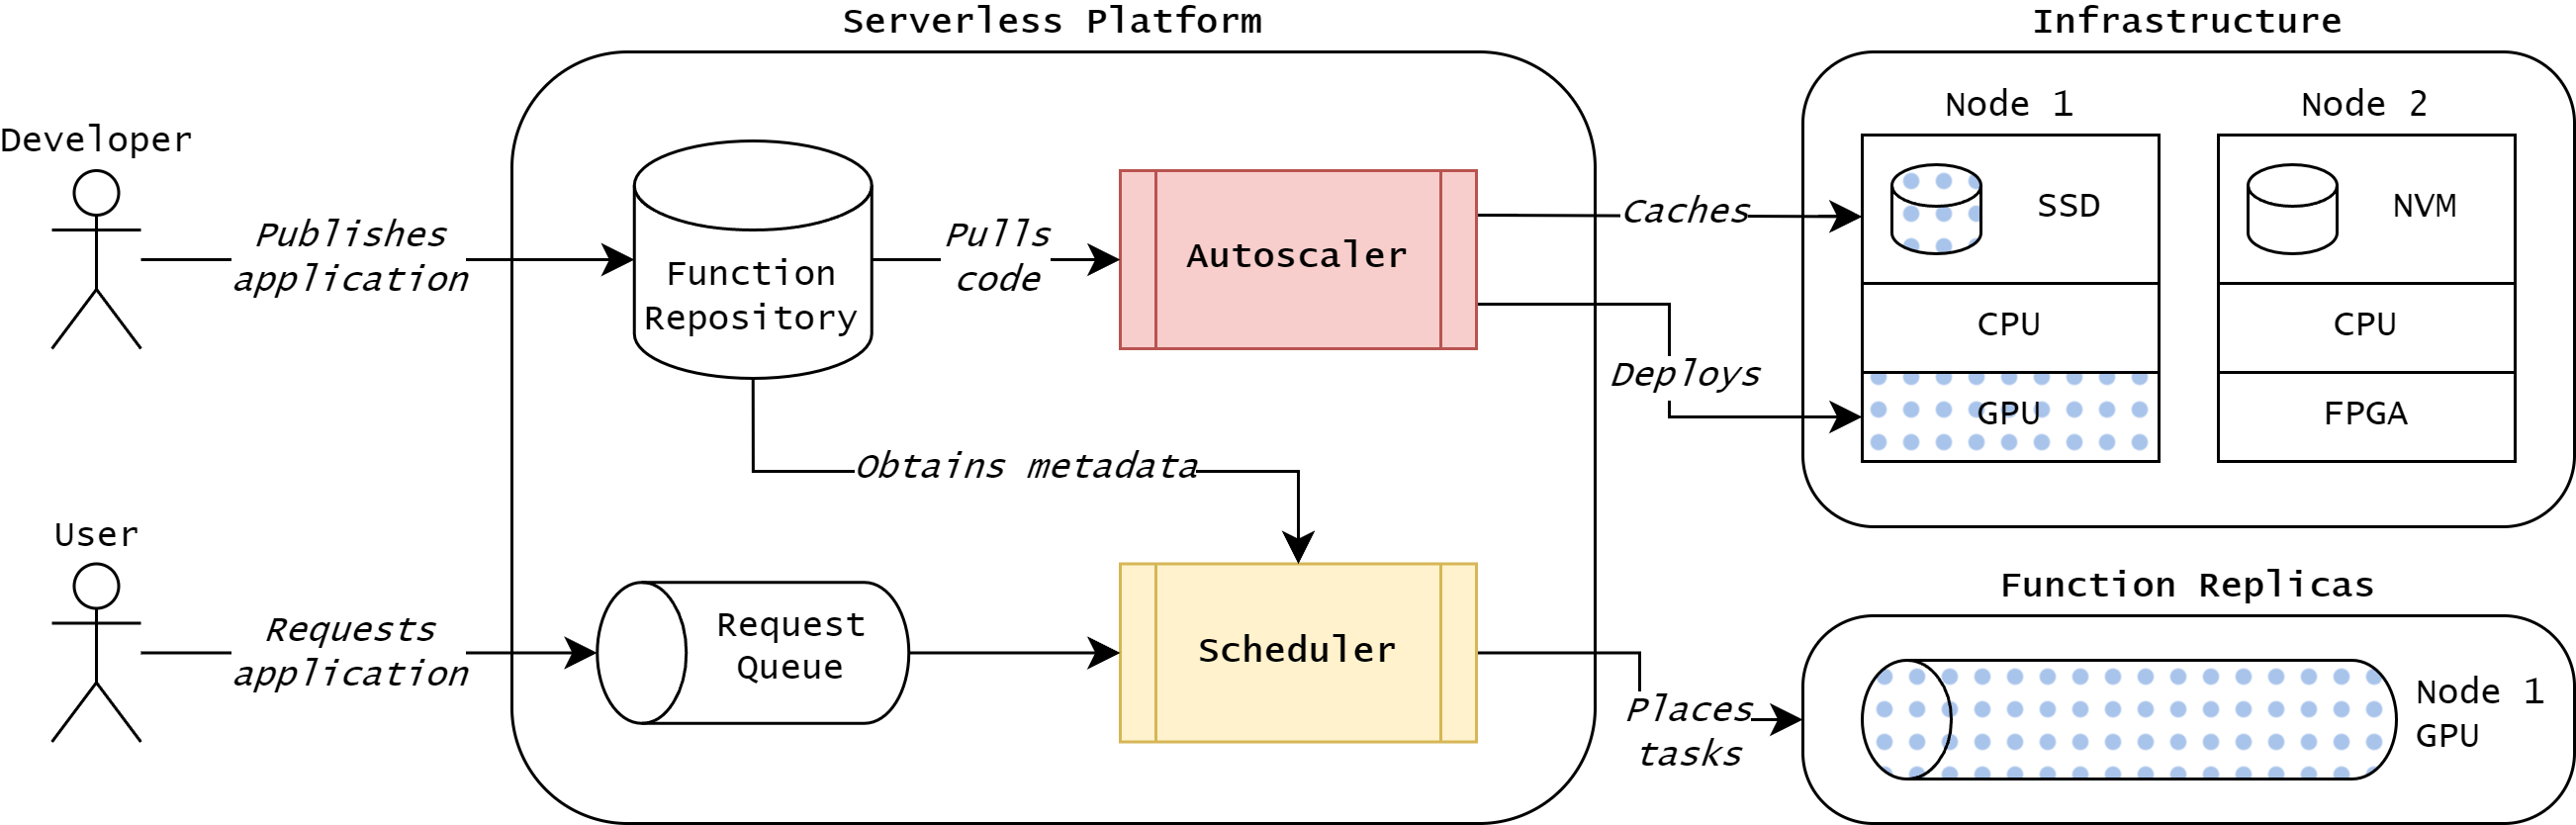
\includegraphics[width=0.9\textwidth]{6_Chapitre6/figures/platform.png}
    \caption{Vue de haut niveau d'une plateforme serverless, telle que modélisée dans HeROsim. L'autoscaler alloue des ressources matérielles pour les répliques de fonctions ; tandis que l'ordonnanceur place les requêtes utilisateur en file d'attente sur ces répliques}.
\label{figure:herosim-platform}
\end{figure*}

Dans le cloud, les clients réservent généralement des ressources. Il s'agit généralement d'un sous-ensemble virtualisé de ressources matérielles hétérogènes disponibles sur des serveurs appelés nœuds. Une fois la réservation effectuée, les fournisseurs de services offrent un accès à distance au client, qui est responsable du déploiement de ses applications et facturé en fonction de la quantité de ressources qu'il a réservées~\cite{Lannurien2023}.

Dans le paradigme serverless, les clients commencent par pousser leur code dans un référentiel du côté du fournisseur, voir la figure~\ref{figure:herosim-platform}. Le fournisseur alloue des ressources qui sont automatiquement mises à l'échelle en fonction de la charge. Pour que ce mécanisme fonctionne, les applications sont divisées en petites unités d'exécution sans état appelées \textbf{fonctions}. Ces fonctions sont sans état : si elles produisent des données de sortie, celles-ci doivent être conservées dans un stockage persistant~\cite{yuFollowingDataNot}.

Dans les modèles de service traditionnels, les ressources sont mises à l'échelle sur deux dimensions : horizontalement (nouvelles instances d'application créées sur d'autres nœuds) et verticalement (ressources supplémentaires allouées aux instances existantes). Dans les plateformes serverless, les ressources sont mises à l'échelle horizontalement : les variations de charge des applications sont absorbées par l'ajout de nouvelles instances des fonctions, appelées \textbf{replicas}, et leur suppression lorsqu'elles ne sont plus nécessaires. Une réplique peut être créée pour chaque requête utilisateur ou réutilisée pour plusieurs requêtes d'utilisateurs. Nous pouvons considérer les répliques de fonctions comme des files d'attente de requêtes ayant des capacités différentes.

Ces répliques sont créées par l'\textbf{autoscaler}. Pour gérer le nombre de répliques déployées pour chaque fonction, il existe trois stratégies principales : basée sur les requêtes, basée sur la concurrence et basée sur les métriques~\cite{mahmoudiSimFaaSPerformanceSimulator2021}. Dans le cadre de l'autoscaling basé sur les requêtes, les requêtes arrivant dans le système sont traitées par des répliques inactives. Si aucune réplique inactive n'est disponible, une nouvelle instance est créée. Dans l'autoscaling basé sur la concurrence, chaque réplique peut mettre en file d'attente plusieurs requêtes d'utilisateurs et les traiter séquentiellement en fonction d'un seuil de concurrence prédéfini~\cite{herofake}. Dans l'autoscaling basé sur les métriques, le nombre de répliques déployées dépend de divers objectifs, tels que le taux de requêtes par seconde (RPS) à atteindre. Pour ce faire, il faut surveiller les performances du système à l'usage de l'autoscaler.

Les répliques peuvent se trouver dans trois états différents : initialisation, exécution et inactivité~\cite{SchleierSmith2021WhatSC}. Lorsqu'une réplique de fonction vient d'être créée, elle est en état d'initialisation : la plateforme instancie son environnement d'exécution, extrait son code d'un registre distant et le met éventuellement en cache sur le nœud de déploiement, puis commence à exécuter la fonction. Lorsque la réplique traite les requêtes utilisateur, elle est en état d'exécution. Dans le cas contraire, la réplique est inactive et peut être supprimée. Lorsque les répliques sont supprimées, les ressources matérielles sont libérées. Toutefois, la création d'une nouvelle réplique pour traiter les requêtes utilisateur entraîne un surcoût appelé \textbf{démarrage à froid}. Les orchestrateurs adoptent diverses politiques pour atténuer ce problème, allant de l'application d'une période de maintien en vie sur les répliques de fonctions pour éviter de les détruire trop tôt, à l'allocation proactive de répliques.

Enfin, les requêtes utilisateur sont attribuées aux répliques de fonctions disponibles par l'\textbf{ordonnanceur} qui met en œuvre différentes stratégies : par exemple AWS Lambda\footnote{\href{https://aws.amazon.com/en/lambda/}{https://aws.amazon.com/en/lambda/}} utilise un algorithme de bin-packing, tandis qu'une plateforme open source telle que Knative met en œuvre une politique d'équilibrage de la charge~\cite{Lannurien2023}. Ces stratégies ont des résultats différents en ce qui concerne l'utilisation des ressources et la qualité de service, mais il peut être difficile de prédire dans quelle mesure elles auront un impact sur les charges de travail avant le déploiement.

\section{Choix de conception}
\label{section:herosim-herosim}

Cette section présente les choix de conception et les hypothèses formulées pour le développement de HeROsim.

\begin{figure}[t]
    \centering
    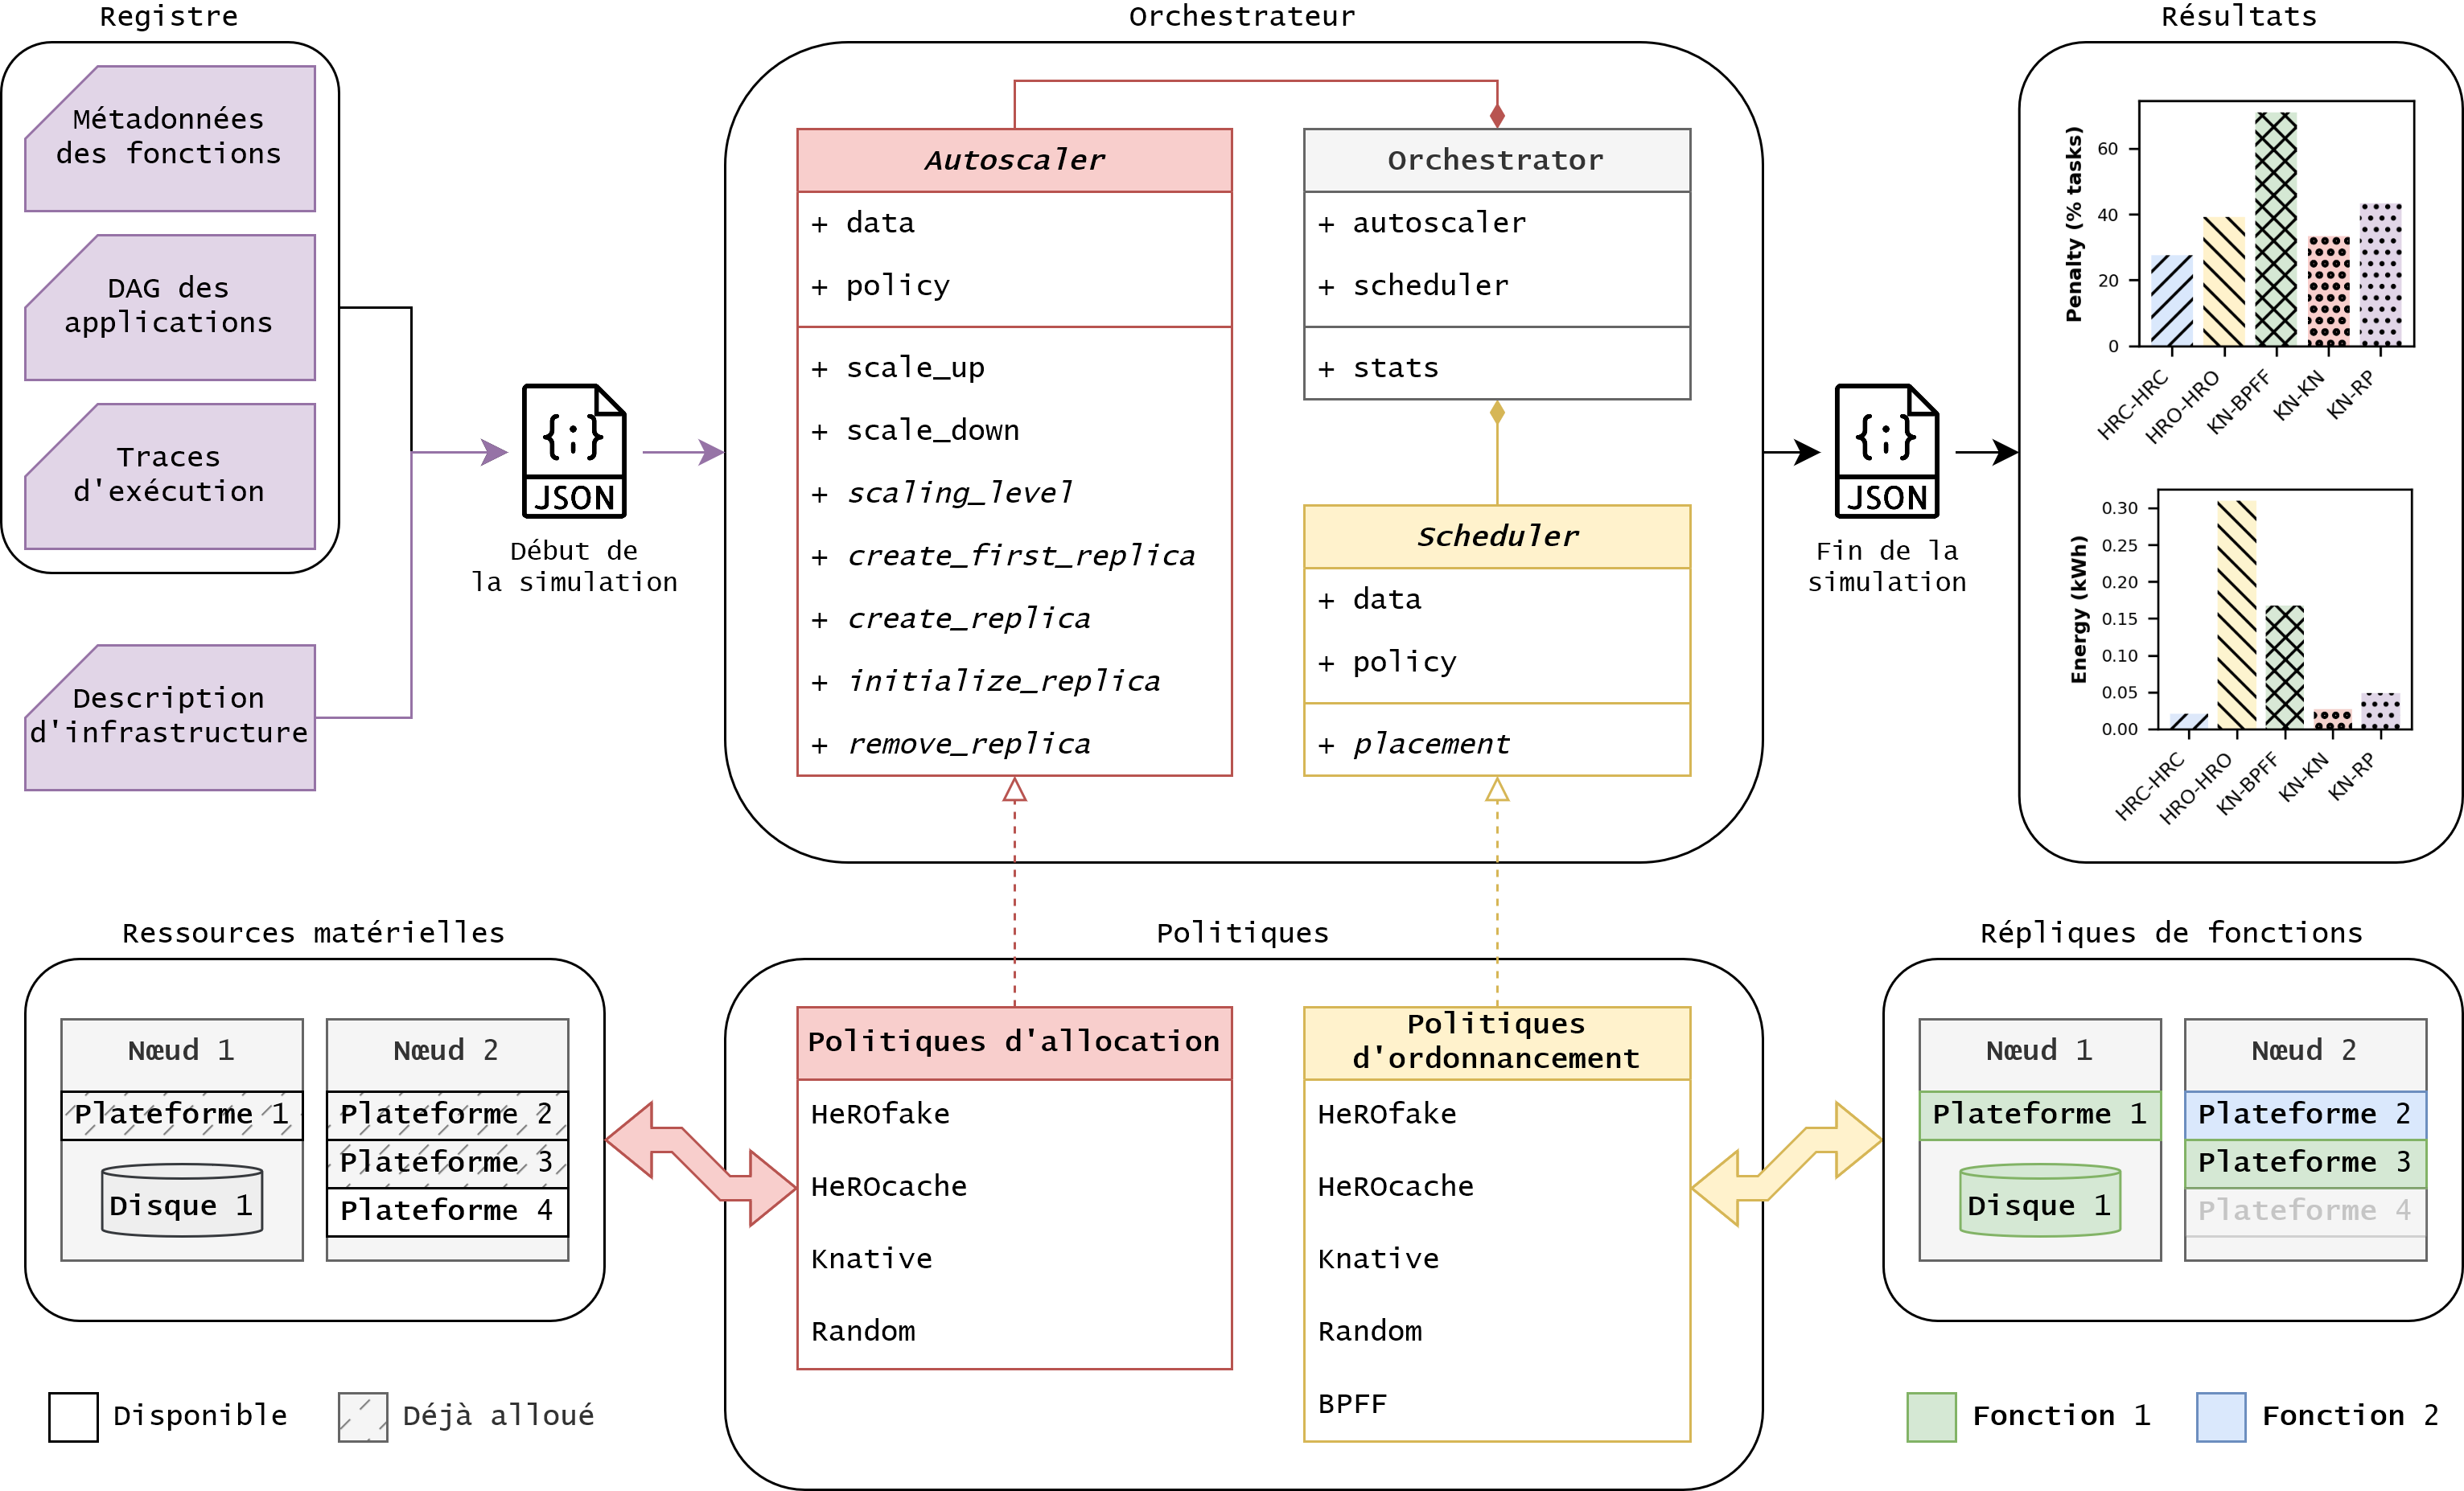
\includegraphics[width=\columnwidth]{6_Chapitre6/figures/software-architecture.png}
    \caption{Vue de haut niveau de l'architecture du simulateur.}
\label{figure:herosim-software-architecture}
\end{figure}

HeROsim utilise la bibliothèque SimPy~\footnote{\href{https://simpy.readthedocs.io}{https://simpy.readthedocs.io}} comme moteur de simulation à événements discrets. Il fournit trois classes de base - \texttt{Orchestrator}, \texttt{Autoscaler} et \texttt{Scheduler} - qui devraient être sous-classées par les utilisateurs désireux d'implémenter leurs propres algorithmes. Comme l'essentiel du comportement de la plateforme est hérité des classes de base, le coût de mise en œuvre d'une nouvelle politique est minime : le couple le plus simple d'autoscaler et d'ordonnanceur (politique de placement aléatoire) est mis en œuvre en moins de 20 lignes de code.

\subsection{Données d'entrée}

HeROsim expose une interface déclarative permettant aux utilisateurs de définir leur environnement cloud, leurs charges de travail et leurs contraintes de qualité de service. Le simulateur reproduit un scénario d'allocation et de placement selon différentes politiques d'orchestration. Une exécution du simulateur nécessite les entrées JSON suivantes pour définir un tel scénario :

\begin{enumerate}
    \item Une \textbf{description des applications} comportant les mesures des des \textbf{caractéristiques des fonctions} invoquées au cours du scénario, \textit{i.e.} leurs temps d'exécution et de démarrage à froid, leurs besoins mémoire, leur consommation d'énergie, la taille de l'image des fonctions, la taille des entrées/sorties lors des phases de communication. Ces métadonnées peuvent être définies en \textbf{mesurant} et \textbf{analysant} le comportement des applications sur une configuration de banc d'essai (voir figure~\ref{figure:herosim-characterization}) ;
    \item Une \textbf{description de l'infrastructure} listant les différents \textbf{nœuds disponibles} et les plateformes d'exécution qu'ils comportent, leurs supports de stockage et la bande passante disponible sur le réseau. Les plateformes d'exécution sont définies en termes de consommation d'énergie au repos et de prix de détail ; les dispositifs de stockage sont caractérisés par leur capacité, leur bande passante et leur latence. Ces données sont spécifiques à une plateforme cible et peuvent être \textbf{mesurées} ou obtenues auprès des fabricants ;
    \item Une \textbf{trace d'exécution} faisant état des temps d'arrivée pour toutes les \textbf{requêtes utilisateur} vers les applications déployées, associées au niveau de qualité de service demandé par l'utilisateur, dans l'ordre chronologique. Ces données peuvent être extraites par \textbf{observations} réelles des applications en production (voir figure~\ref{figure:herosim-characterization}), ou estimées statistiquement.
\end{enumerate}

Les données de nos études précédentes~\cite{herofake, herocache} sont disponibles dans le référentiel pour référence. Alors que (1) et (2) peuvent être rédigés à la main en fonction des exigences du cas d'utilisation, HeROsim fournit un générateur synthétique pour créer diverses traces pour (3) en utilisant des processus de Poisson, avec une durée variable et un taux requêtes par seconde, comme cela est couramment fait dans la littérature~\cite{herocache}. 

\subsection{Flot d'une simulation}

L'utilisateur peut choisir les politiques d'orchestration souhaitées et exécuter le programme principal. Le simulateur :

\begin{itemize}
    \item Initialise l'infrastructure comme décrit : le scénario commence avec tous les nœuds inactifs, en attente de nouvelles requêtes ;
    \item Initialise l'orchestrateur avec l'autoscaler et l'ordonnanceur choisis ;
    \item Suit les temps d'arrivée des événements à partir de la trace d'exécution et transmet les requêtes utilisateur à l'orchestrateur ;
    \item Laisse l'ordonnanceur essayer de placer ces requêtes sur des répliques de fonctions ;
    \item Laisse l'autoscaler allouer et désallouer les ressources matérielles qui hébergent ces répliques pour traiter les requêtes utilisateur.
\end{itemize}

La simulation progresse dans le traitement des requêtes utilisateur. Le simulateur connaît le temps de réponse des fonctions sur la base des métadonnées d'entrée mesurées au préalable. Ces métadonnées concernent le matériel et les charges de travail spécifiques que l'utilisateur souhaite ordonnancer. Elles peuvent être obtenues de différentes manières ; la figure~\ref{figure:herosim-characterization} donne un aperçu de la méthodologie que nous avons utilisée pour caractériser les différentes charges de travail et plates-formes d'exécution tout au long de nos expériences ; voir~\cite{herofake, herocache} pour plus de détails.

\begin{figure}[t]
    \centering
    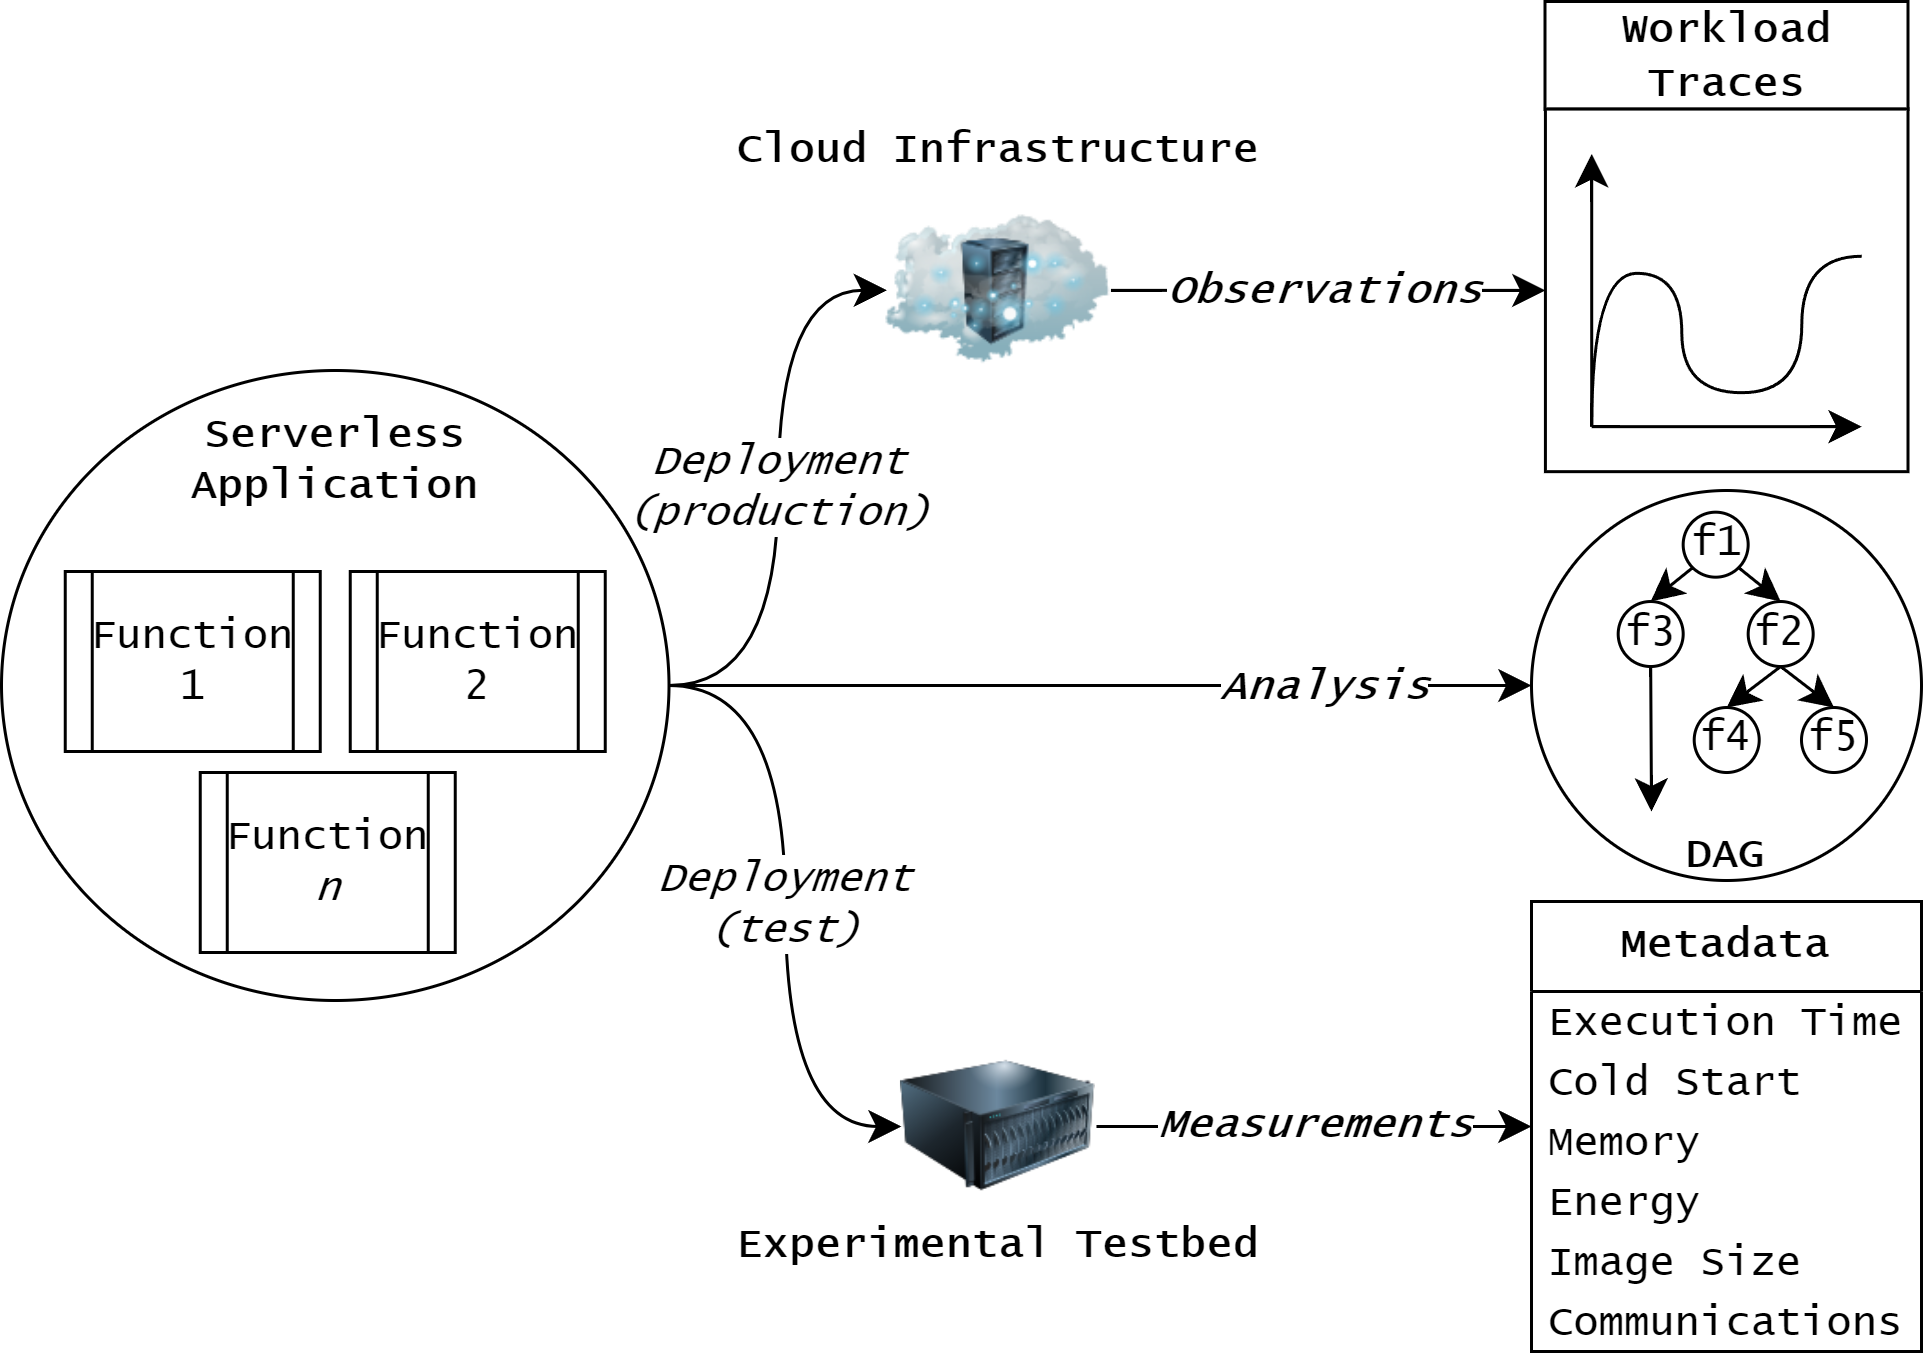
\includegraphics[width=\columnwidth]{6_Chapitre6/figures/characterization.png}
    \caption{Une vue d'ensemble de notre méthodologie de caractérisation.}
\label{figure:herosim-characterization}
\end{figure}

Pendant la simulation, les journaux sont écrits sur le disque. Lorsque toutes les requêtes utilisateur ont été traitées, la simulation s'arrête et renvoie les résultats et les graphiques résumant la simulation, respectivement dans les répertoires \texttt{result} et \texttt{chart}.

Le simulateur est monotâche, ce qui signifie que chaque politique sera évaluée de manière séquentielle. Cependant, plusieurs instances de HeROsim peuvent être exécutées en parallèle avec différentes configurations sur plusieurs cœurs de CPU, ou distribuées sur plusieurs nœuds. Chaque instance de HeROsim exécutant une politique d'orchestration différente et toutes les instances utilisant un répertoire de sortie commun, cela peut accélérer la durée totale du scénario de simulation lors de l'évaluation de nombreuses politiques d'orchestration. Lorsque toutes les exécutions du simulateur sont terminées, les résultats peuvent être consolidés dans un seul tableau de sortie.

\subsection{Orchestrateur}

La classe de base \textbf{\texttt{Orchestrator}} fournit des méthodes d'initialisation abstraites qui doivent être surchargées pour gérer différentes structures de l'état du système. Par exemple, un ordonnanceur Round Robin devra savoir combien de fois chaque réplique de fonction a été sélectionnée pour le placement des tâches, tandis qu'un ordonnanceur Least Connected devra connaître la concurrence moyenne dans chaque réplique pour équilibrer la charge. Cette classe est le point d'entrée permettant aux utilisateurs de définir leurs propres structures de données qui représenteront au mieux l'état du système à gérer par l'autoscaler et l'ordonnanceur.

Les utilisateurs peuvent mettre en œuvre le processus de gestion de l'état du système dont ils ont besoin pour soutenir leurs politiques d'orchestration. L'orchestrateur de base est doté d'un système simple qui peut fonctionner tel quel ou être étendu. Dans notre implémentation, un processus de surveillance est appelé périodiquement pour garder une trace de la concurrence moyenne dans chaque réplique de fonction. Ceci est utile pour les politiques basées sur des seuils.

La méthode du point d'entrée de l'orchestrateur est appelée chaque fois qu'une requête utilisateur arrive sur la plateforme. Elle prend en entrée l'état du système et la requête utilisateur. Elle peut être surchargée dans chaque implémentation de politique d'orchestration pour permettre une mise à l'échelle automatique et une ordonnanceur à grain fin selon les besoins.

Enfin, cette classe est responsable de l'instanciation des implémentations sélectionnées pour \texttt{Autoscaler} et \texttt{Scheduler}. Toute combinaison de ces deux modules peut être instanciée.

\subsection{Allocateur}

La classe de base \textbf{\texttt{Autoscaler}} fournit le comportement commun de la plateforme d'autoscaling, y compris la création et la suppression des répliques de fonctions. Plusieurs méthodes abstraites doivent être remplacées pour mettre en œuvre une nouvelle politique : sélection des ressources pour la création de répliques, processus d'initialisation des répliques, sélection des répliques pour la suppression, etc. Ces méthodes opèrent à la granularité d'une seule fonction, en prenant l'état du système et la liste des ressources matérielles disponibles comme données d'entrée. Les utilisateurs sont libres de mettre en œuvre les algorithmes qu'ils souhaitent évaluer pour la gestion des ressources.

L'autoscaler de HeROsim a été principalement conçu pour une mise à l'échelle horizontale. Les répliques de fonctions sont créées en allouant une plateforme d'exécution et la quantité requise de mémoire de crête sur un nœud. Une plateforme d'exécution ne peut pas héberger plus d'une réplique de fonction à la fois. Pour faire face à l'augmentation de la charge d'une application sans dégradation de la qualité de service, de nouvelles répliques de fonctions doivent être allouées par l'autoscaler, à condition qu'il y ait suffisamment de ressources matérielles disponibles. Les répliques nouvellement allouées passent par une phase d'initialisation au cours de laquelle les images des fonctions doivent être récupérées via le réseau. L'autoscaler peut gérer un cache d'images dans la mémoire du nœud et sur le stockage local du nœud afin d'accélérer les démarrages à froid.

La suppression des répliques inactives se fait au mieux : l'autoscaler tente de supprimer les répliques dont les files d'attente de tâches sont vides. Par défaut, une réplique avec des tâches en attente ne peut pas être supprimée.

L'autoscaler garde une trace de chaque événement d'allocation pour calculer l'utilisation des ressources à la fin de la simulation. HeROsim permet à l'utilisateur de savoir quels nœuds et quelles plates-formes d'exécution ont été enrôlés pendant le scénario, à quel moment et pour quelle durée, et pour quel déploiement de fonction ils ont été choisis. Cela permet également à HeROsim de calculer la consommation d'énergie à différentes granularités : la puissance statique nécessaire au matériel alloué et la puissance dynamique utilisée par les applications pendant leur exécution.

HeROsim est livré avec les politiques de mise à l'échelle automatique suivantes, basées sur des seuils de concurrence et prêtes à l'emploi :

\begin{itemize}
    \item Random -- Sélectionne un nœud aléatoire et une plateforme d'exécution pour les nouvelles répliques ;
    \item Knative -- Sélectionne le nœud le moins chargé pour allouer de nouvelles répliques, \textit{i.e} équilibre les charges de travail sur un grand nombre de nœuds ;
    \item HeROfake -- Exploite l'hétérogénéité du matériel pour minimiser les pénalités de qualité de service, la consommation d'énergie et le coût total de possession. Plus de détails sont donnés dans la section "Étude de cas" ;
    \item HeROcache -- Optimise les allocations pour les chaînes de fonctions ; maximise les fonctions de consolidation de chaque application. Plus de détails sont donnés dans la section "Étude de cas".
\end{itemize}

\subsection{Ordonnanceur}

La classe de base \textbf{\texttt{Scheduler}} met en œuvre la sélection des tâches dans la file d'attente de la passerelle. Une méthode abstraite doit être surchargée pour mettre en œuvre une nouvelle politique : la sélection d'une réplique parmi le pool pour placer chaque requête utilisateur dans la file d'attente. Cette méthode opère à la granularité d'une requête utilisateur et prend en entrée l'état du système et la liste des répliques de fonctions disponibles.

Les requêtes utilisateur arrivent dans une file d'attente au niveau de l'ordonnanceur. Les utilisateurs peuvent mettre en œuvre leur propre politique de priorité pour la sélection des tâches ou choisir une politique déjà disponible dans le simulateur, \textit{e.} FIFO ou Earliest Deadline First~\cite{herofake}.

L'ordonnanceur de HeROsim a été conçu sans tenir compte des défaillances ou des migrations de tâches : le comportement par défaut considère les tâches qui s'exécutent toujours jusqu'à leur terme sur leur réplique. Cependant, les tâches seront marquées comme "en pénalité" si l'ordonnanceur manque son échéance. Les utilisateurs peuvent utiliser cette valeur booléenne pour évaluer la qualité de leurs politiques en ce qui concerne la latence des requêtes : elle indique la proportion de requêtes qui sont traitées en temps voulu. 

S'il n'y a pas de réplique disponible au moment de l'ordonnancement d'une requête utilisateur, l'ordonnanceur fera un appel à l'autoscaler pour forcer la création d'une première réplique pour la fonction. Dans l'intervalle, la requête est remise dans la file d'attente et reportée. Les tâches reportées sont signalées comme telles, de sorte que, par exemple, elles peuvent avoir une priorité plus élevée si l'utilisateur souhaite appliquer une telle politique~\cite{herocache}.

HeROsim est livré avec les politiques d'ordonnanceur suivantes implémentées et prêtes à l'emploi :

\begin{itemize}
    \item Random -- Sélectionne une réplique aléatoire pour le placement des tâches ;
    \item Knative -- Sélectionne la réplique avec la file d'attente la plus courte pour le placement des tâches ;
    \item BPFF -- Sélectionne la réplique avec la plus longue file d'attente de requêtes en vol pour le placement des tâches ;
    \item HeROfake -- Sélectionne la réplique qui minimise un score composé en fonction de l'échéance de la tâche, de la consommation d'énergie de la fonction et de la dispersion des tâches sur les nœuds. Plus de détails sont donnés dans la section "Étude de cas" ;
    \item HeROcache -- Sélectionne la réplique similaire à HeROfake, mais prend en compte les opérations de stockage et de communication pour calculer la latence de bout en bout de la requête, et prend en compte les chaînes de fonctions lors de l'évaluation des répliques en ce qui concerne la consolidation des tâches. De plus amples détails sont donnés dans la section "Étude de cas".
\end{itemize}


\subsection{Interface utilisateur}

HeROsim s'appuie sur la journalisation pour fournir un aperçu du déroulement de la simulation, ce qui aide l'utilisateur à déboguer ses politiques. À la fin de la simulation, les fichiers de résultats sont enregistrés sur le disque. Ces fichiers contiennent des informations sommaires sur les résultats de la simulation, y compris les performances de la politique en ce qui concerne les mesures d'évaluation. Ces résultats sont représentés sur différents graphiques qui peuvent être utilisés dans des publications ultérieures (voir figure~\ref{figure:herosim-evaluation}).

HeROsim peut également générer des graphiques supplémentaires qui peuvent être utiles lors du débogage du comportement d'une politique d'orchestration. Les utilisateurs peuvent visualiser la proportion de démarrages à froid et d'accès au cache parmi les invocations de fonctions. HeROsim peut tracer la latence de la queue pour toutes les requêtes des utilisateurs, aidant ainsi l'utilisateur à dimensionner son infrastructure. Le générateur de traces d'exécution trace les temps d'arrivée des requêtes sur un graphique afin de fournir des indications visuelles sur les caractéristiques de la charge de travail.

\begin{figure}[t]
    \centering
    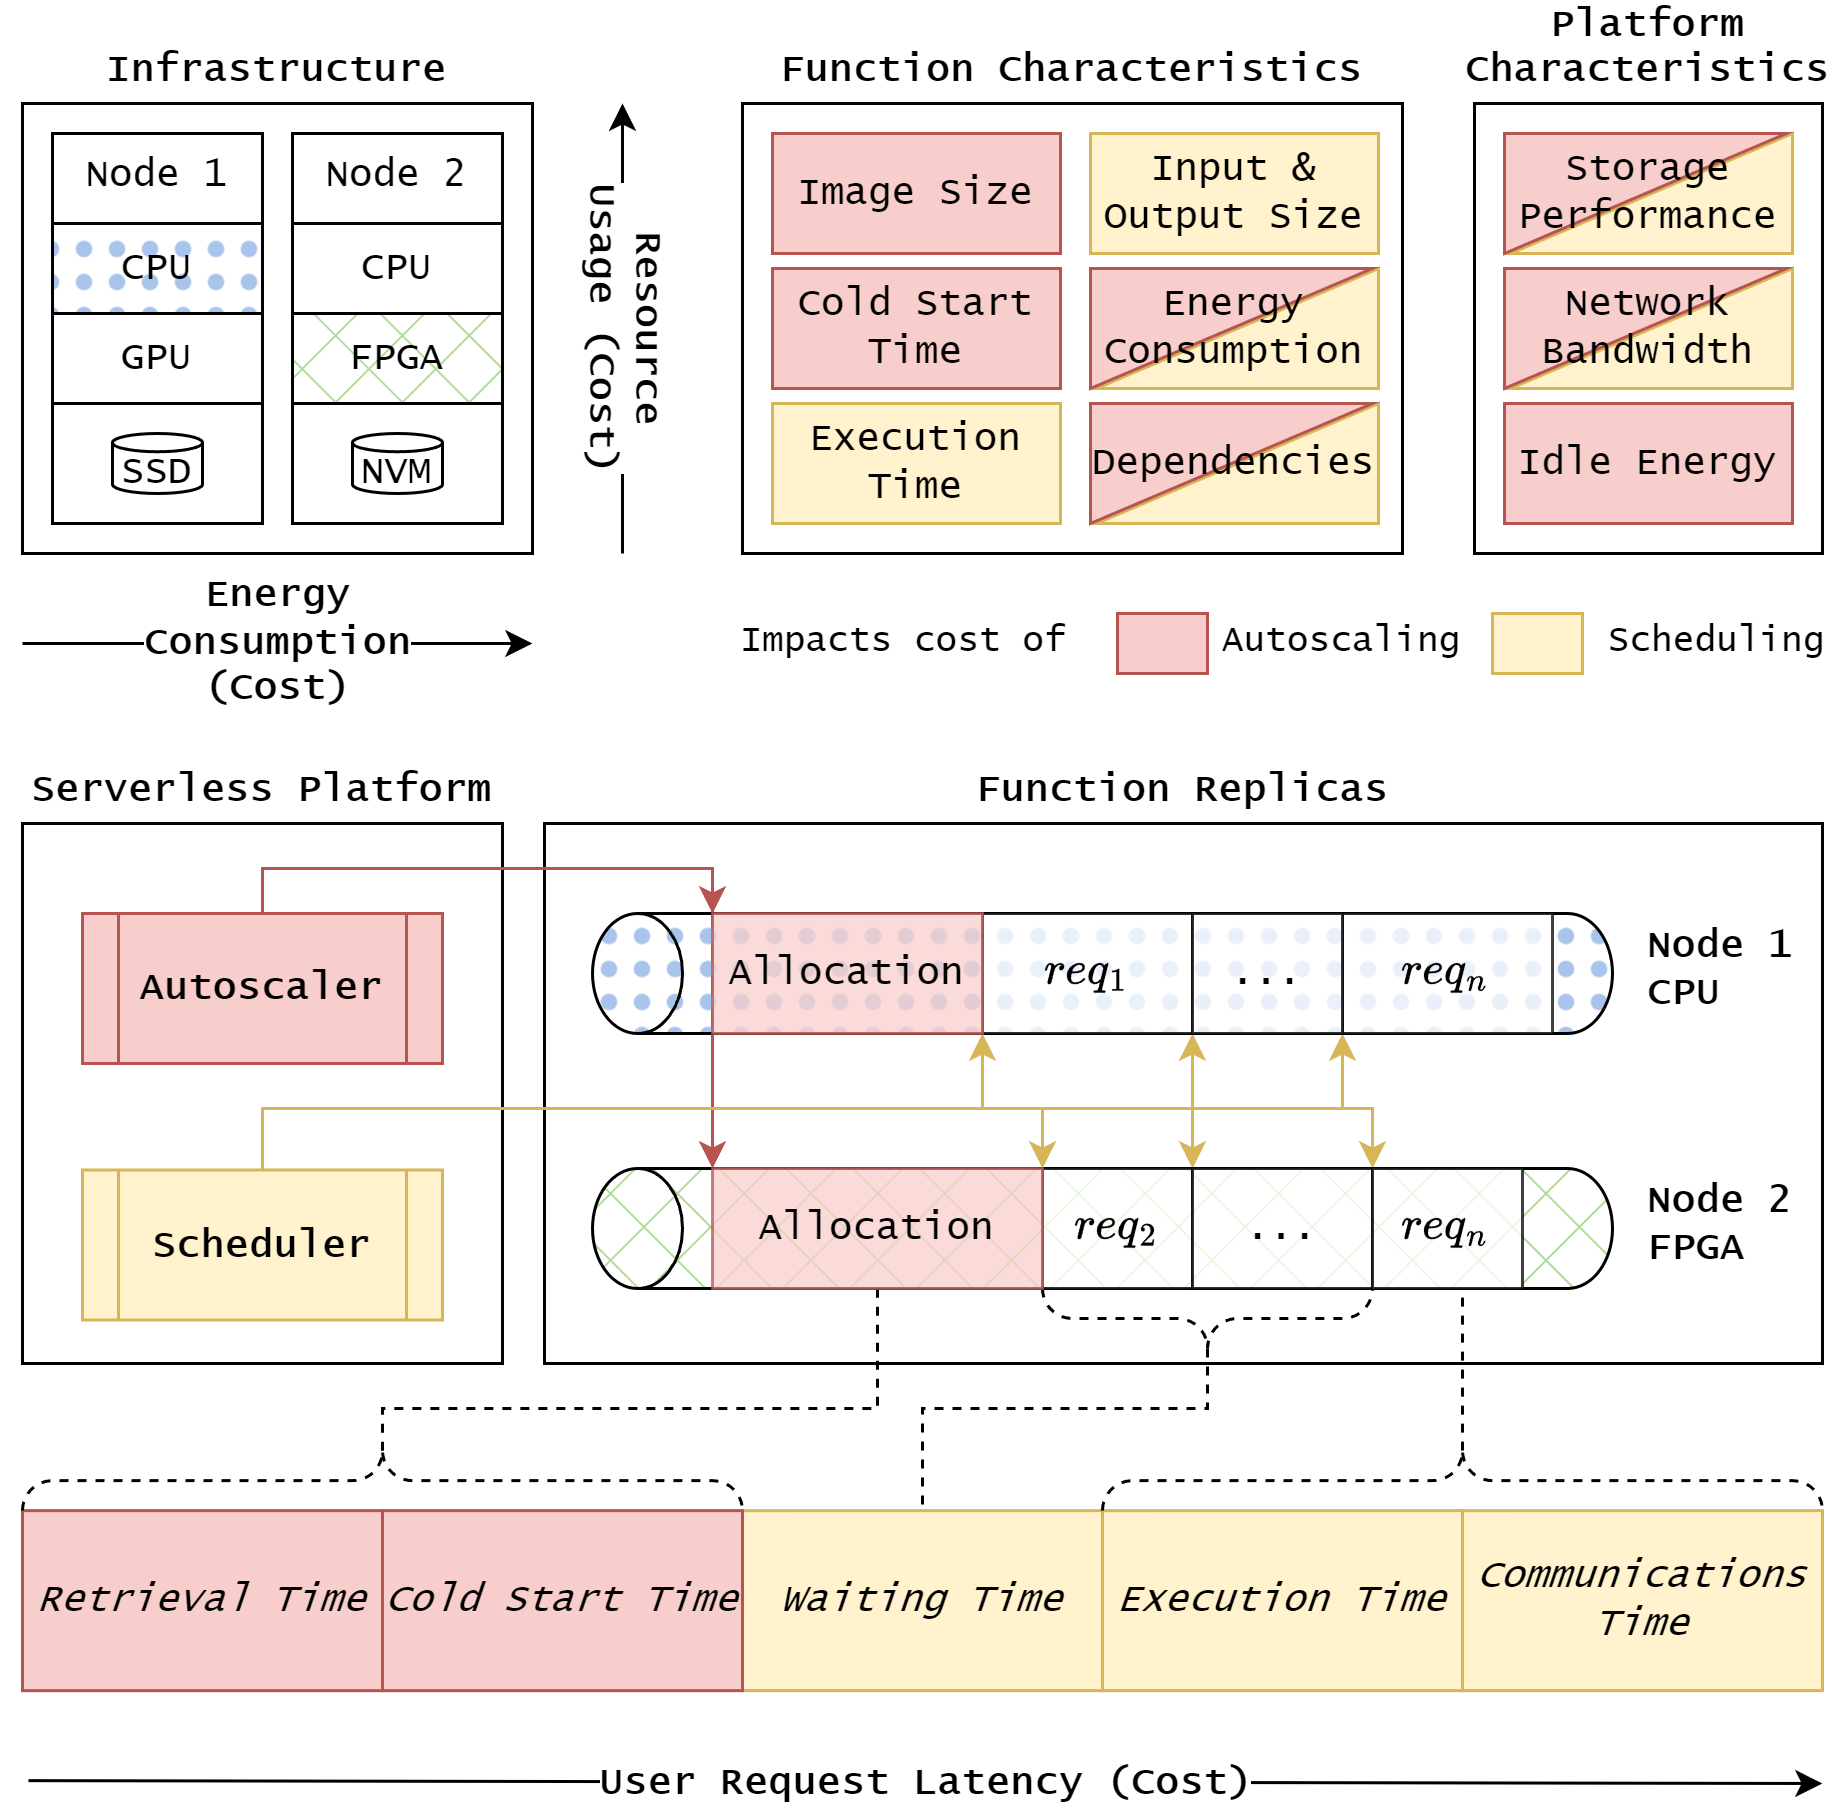
\includegraphics[width=\columnwidth]{6_Chapitre6/figures/serverless-cost.png}
    \caption{Répartition du coût de latence de bout en bout induit par les décisions d'autoscaling et d'ordonnancement.}
\label{figure:herosim-cost}
\end{figure}

\section{Étude de cas}
\label{section:herosim-case-study}

\begin{figure*}[t]
    \center
    \subfloat[Consolidation\label{figure:herosim-evaluation-full-unused-nodes}]{
        \includegraphics[width=0.155\linewidth]{6_Chapitre6/figures/eval/2-unused-nodes.png}
    }
    \subfloat[QoS\label{figure:herosim-evaluation-full-penalty}]{
        \includegraphics[width=0.155\linewidth]{6_Chapitre6/figures/eval/3-penalty-proportions.png}
    }
    \subfloat[Energy\label{figure:herosim-evaluation-full-energy-consumption}]{
        \includegraphics[width=0.155\linewidth]{6_Chapitre6/figures/eval/6-energy-consumption.png}
    }
    \subfloat[Consolidation\label{figure:herosim-evaluation-components-unused-nodes}]{
        \includegraphics[width=0.155\linewidth]{6_Chapitre6/figures/eval-components/2-unused-nodes.png}
    }
    \subfloat[QoS\label{figure:herosim-evaluation-components-penalty}]{
        \includegraphics[width=0.155\linewidth]{6_Chapitre6/figures/eval-components/3-penalty-proportions.png}
    }
    \subfloat[Energy\label{figure:herosim-evaluation-components-energy-consumption}]{
        \includegraphics[width=0.155\linewidth]{6_Chapitre6/figures/eval-components/6-energy-consumption.png}
    }
    \caption{Charts generated by HeROsim for the evaluation of HeROcache -- Comparison against baselines (a-c) and impact of individual components (d-f). HRC-HRO means HeROcache autoscaler coupled with HeROfake scheduler.}
    \label{figure:herosim-evaluation}
\end{figure*}

Nous présentons deux études de cas qui ont utilisé HeROsim pour évaluer les politiques d'orchestration.
Nous avons conçu des stratégies qui reposent sur la caractérisation des plateformes hétérogènes et des charges de travail (voir figure~\ref{figure:herosim-characterization}). Nous avons mesuré plusieurs métriques liées à nos applications sur diverses plateformes matérielles et proposé un modèle de coût qui intègre ces valeurs pour estimer les performances de l'autoscaling et de l'ordonnanceur sous différentes politiques (figure~\ref{figure:herosim-cost}).

\subsection{Stratégie d'orchestration de fonctions sans état sur ressources hétérogènes}

Dans cette première étude de cas, \textbf{He}terogeneous \textbf{R}esources \textbf{O}rchestration for deep\textbf{fake} detection~\cite{herofake}, nous avons étudié le déploiement d'une application de détection de deepfake sur une plateforme serverless dans un cloud privé. En particulier, nous nous sommes intéressés à l'exploitation de ressources hétérogènes pour l'orchestration serverless lors de l'optimisation de la plateforme pour la QoS et la consommation d'énergie.

L'application exécute des tâches d'inférence pour détecter les deepfakes dans des images potentiellement trafiquées, soumises par des utilisateurs avec diverses exigences de niveau de QoS. Son objectif est de détecter les images potentiellement falsifiées, c'est-à-dire les images susceptibles d'avoir été manipulées par ordinateur pour tromper les spectateurs. Il se compose de trois tâches de réseau neuronal indépendantes et sans état qui ont été mises en œuvre sur du matériel hétérogène : CPU, GPU et FPGA. Ces implémentations ont été utilisées pour les mesures, mais il aurait été difficile d'exécuter réellement des scénarios du monde réel sur une plateforme serverless incluant ces architectures matérielles.

Dans HeROfake, chaque exécution de tâche a un coût associé mesuré en \textbf{latence}. L'allocation de nouvelles répliques sur des ressources matérielles inactives introduit un \textbf{délai de démarrage à froid} ; le traitement des requêtes utilisateur sur différents matériels a divers \textbf{temps d'exécution de la fonction}. La latence de chaque requête utilisateur est finalement comparée à la \textbf{exigence de qualité de service} de la requête : si l'échéance de la requête n'a pas été respectée, la tâche est en \textbf{pénalité}. Ces éléments constituent la base de notre modèle de coût, voir la figure~\ref{figure:herosim-cost}.

Les différentes architectures matérielles ont également des coûts monétaires et énergétiques différents qui ont été pris en compte dans le modèle de coût. Nous avons mis en œuvre un autoscaler et un ordonnanceur qui cherchent à estimer et à minimiser ce coût composite à la granularité de chaque requête utilisateur. L'autoscaler cherche à allouer des plateformes qui minimisent le coût global, y compris l'utilisation des ressources, la consommation d'énergie et le coût total de possession. L'ordonnanceur cherche à sélectionner les répliques qui traitent les requêtes avec le moins de pénalités et la plus faible consommation d'énergie.

HeROfake a été évalué à l'aide d'un scénario synthétique avec une distribution uniforme des temps d'arrivée des requêtes, des appels de fonction et des niveaux de qualité de service. HeROfake s'est avéré performant (en termes de pénalités de QoS, de consolidation et d'énergie) par rapport à Knative (l'orchestrateur serverless de Google) et Bin-Packing First Fit (la politique d'Amazon dans Lambda)~cite{herofake}. 

Notre objectif principal était d'étudier la pertinence de la prise en compte de l'hétérogénéité matérielle lors de l'allocation des ressources et de l'ordonnancement des requêtes utilisateur en ce qui concerne diverses mesures de qualité de service, \textit{i.e.} la latence de bout en bout et la consommation d'énergie. Les résultats expérimentaux ont montré que si le temps total d'exécution des tâches dans HeROfake est similaire à celui de la version vanille de Knative, nous obtenons une réduction de plus de 60\% des pénalités de qualité de service ; les tâches sont consolidées sur moins de 40\% des nœuds de l'infrastructure, 77\% des plates-formes d'exécution restant inutilisées ; et la consommation d'énergie dynamique est réduite de 35\% par rapport à Knative.

HeROsim nous a également permis d'évaluer l'impact des différents composants de notre cadre. Les résultats ont montré que, même en allouant uniquement des CPU, l'ordonnanceur des tâches d'inférence avec notre politique consciente de la qualité de service pouvait maintenir les violations des accords de niveau de service en dessous de 50\%. 

\subsection{Stratégie d'orchestration d'applications avec prise en compte du cache et des communications}

Ici, une stratégie d'orchestration consciente des contraintes temporelles et de données a été proposée. Nous avons exploré le déploiement d'un système de détection d'intrusion (IDS) sur une plateforme serverless. En particulier, nous avons étudié les avantages de l'orchestration consciente des données lors de l'exploitation de matériel hétérogène pour déployer des applications sensibles au temps sur des dispositifs périphériques à ressources limitées, du point de vue du fournisseur de services.

L'objectif de l'application est de détecter le trafic TCP potentiellement malveillant dans les journaux de réseau soumis par les utilisateurs. Comme cette application IDS est spécifiquement destinée aux missions de drones, son schéma d'accès est étroitement lié aux schémas saisonniers, ce qui en fait une bonne adaptation au paradigme serverless.

L'application se compose de deux couches : deux fonctions de prétraitement qui opèrent sur les journaux du trafic réseau, et quatre fonctions d'inférence qui détectent des modèles d'activité malveillante dans les journaux. Ces fonctions ont été mises en œuvre sur différentes architectures matérielles (CPU, FPGA, GPU). 

Il existe des dépendances de données entre les deux couches de l'application. Nous les avons modélisées sous forme de graphes acycliques dirigés (DAG) d'appels de fonctions. Nous avons utilisé le module Python \texttt{TopologicalSorter} du module \texttt{graphlib} pour la représentation JSON des graphes et pour les parcourir pendant l'exécution.

Au niveau de l'orchestrateur, nous avons dû modifier la granularité des requêtes utilisateur : une requête concerne une application, qui peut être composée d'une ou plusieurs fonctions, appelées dans l'ordre défini par le DAG de l'application. Chaque fonction peut prendre des données en entrée et produire des données en sortie. Ces données sont définies par leur taille en octets.

Alors que HeROfake ne prend pas en compte les opérations de stockage, HeROcache met en œuvre la \textbf{récupération des images de fonctions}, \textbf{la mise en cache des images de fonctions} et les \textbf{communications entre fonctions} dans l'orchestrateur de base. Ces opérations augmentent la latence de la requête utilisateur d'une quantité de temps calculée sur la base de la caractérisation de la plateforme et de la fonction, voir figure~\ref{figure:herosim-cost} : par exemple, HeROsim estime le temps de récupération de l'image de la fonction sur la base de la largeur de bande du réseau spécifiée par l'utilisateur dans la description de l'infrastructure, la taille de l'image de la fonction spécifiée par le type de charge de travail, et la performance du stockage local du nœud spécifiée par le type de stockage.

L'introduction d'opérations de stockage au niveau du nœud individuel nous a permis d'évaluer une stratégie de préchargement d'images de fonctions afin d'accélérer les démarrages à froid dans les invocations futures.

Dans HeROcache, l'autoscaler cherche à accroître la consolidation des fonctions entre les applications, à réduire le makespan global, la consommation d'énergie et le coût total de possession. L'ordonnanceur cherche à éviter le non-respect des délais des requêtes, à consommer moins d'énergie et à assurer une utilisation élevée des ressources.

Nous avons utilisé le générateur de traces d'exécution inclus dans HeROsim pour générer un scénario de 30 minutes de requêtes utilisateur suivant un processus de Poisson à un taux moyen de 83 requêtes par seconde. Cela correspond au taux de communication que la connectivité 4G LTE permettrait dans notre environnement périphérique, compte tenu de la taille des données d'entrée et de sortie de l'application. 

HeROfake exploite déjà l'hétérogénéité matérielle, mais est conçu comme une politique sans stockage, ce qui en fait une solution comparable. Cette comparaison nous a permis de montrer l'importance des coûts de stockage dans le respect de la qualité de service : avec une politique d'orchestration tenant compte des données, HeROcache consolide les applications et parvient à réduire les délais d'initialisation moyens de 17,6 % et les délais de communication de 88,4 %. Cela permet de réduire la consommation d'énergie statique de la plateforme de 80 % tout en maintenant moins de 28 % de violations de la qualité de service.

HeROcache (mis en œuvre au-dessus de HeROsim) a été soumis à l'évaluation des artefacts et a reçu les trois badges de reproductibilité de l'IEEE~\footnote{\href{https://www.niso.org/standards-committees/reproducibility-badging}{https://www.niso.org/standards-committees/reproducibility-badging}} : Open Research Objects (ORO), Reusable/Research Objects Reviewed (ROR), et Results Reproduced (ROR-R).

\section{Travaux connexes}
\label{section:herosim-sota}

\begin{table*}[t]
    \centering
    \caption{Overview of simulation tools for cloud computing}
    \resizebox{\linewidth}{!}{
        \begin{tabular}{lSSSSSSSSS}
        \toprule
        & Serverless & Deployment models & Functions chains & Hardware heterogeneity & Per-request QoS & Resource usage & Energy consumption & Visualization \\
        \cmidrule(lr){2-2}\cmidrule(lr){3-3}\cmidrule(lr){4-4}\cmidrule(lr){5-5}\cmidrule(lr){6-6}\cmidrule(lr){7-7}\cmidrule(lr){8-8}\cmidrule(lr){9-9}
        CloudSim~\cite{calheiros_cloudsim_2011} & \xmark & Public, private, hybrid & \xmark & \cmark & \xmark & \cmark & \cmark & \xmark \\
        CloudSimSC~\cite{mampage_cloudsimsc_2023} & \cmark & Public, private, hybrid & \xmark & \cmark & \xmark & \cmark & \cmark & \xmark \\
        CloudAnalyst~\cite{wickremasinghe_cloudanalyst_2010} & \xmark & Public, private, hybrid & \xmark & \cmark & \xmark & \cmark & \cmark & \cmark \\        DFaaSCloud~\cite{jeonCloudSimExtensionSimulatingDistributed2019} & \cmark & Multi-tier hybrid cloud & \xmark & \xmark & \cmark & \cmark & \xmark & \cmark \\
        ElasticSim~\cite{cai_elasticsim_2017} & \xmark & Public & \cmark & \xmark & \xmark & \cmark & \xmark & \cmark \\
        GridSim~\cite{buyyaGridSimToolkitModeling2002} & \xmark & Grid & \xmark & \cmark & \cmark & \cmark & \xmark & \cmark \\
        iCanCloud~\cite{nunez_icancloud_2012} & \xmark & Public & \xmark & \xmark & \xmark & \cmark & \xmark & \cmark \\
        iFogSim2~\cite{mahmudIFogSim2ExtendedIFogSim2021} & \xmark & Edge, Fog & \xmark & \cmark & \xmark & \cmark & \cmark & \xmark \\
        OpenDC 2.0~\cite{mastenbroekOpenDCConvenientModeling2021} & \cmark & Public, private, hybrid & \cmark & \cmark & \xmark & \cmark & \cmark & \cmark \\
        SimFaaS~\cite{mahmoudiSimFaaSPerformanceSimulator2021} & \cmark & Public & \xmark & \xmark & \xmark & \cmark & \cmark & \cmark \\
        \textbf{HeROsim} & \cmark & Private & \cmark & \cmark & \cmark & \cmark & \cmark & \cmark \\
        \bottomrule
        \end{tabular}
    }
    \label{table:herosim-sota}
\end{table*}

Nous présentons un aperçu des travaux de l'état de l'art et de leurs caractéristiques dans le Tableau~\ref{table:herosim-sota}.

CloudSim~\cite{calheiros_cloudsim_2011} est l'outil omniprésent pour les expériences de déploiement de nuages à grande échelle. Il cible les différents modèles de service traditionnels dans le cloud.
CloudSim, et ses extensions~\cite{calheiros_cloudsim_2011, mampage_cloudsimsc_2023, wickremasinghe_cloudanalyst_2010, jeonCloudSimExtensionSimulatingDistributed2019} ne prennent pas en compte les applications serverless, \textit{i. e.} la composition de fonctions pour obtenir un comportement complexe qui introduit des défis spécifiques (délais de démarrage à froid, frais généraux liés aux communications inter-fonctions, etc.~\cite{wawrzoniakBoxerDataAnalytics2021a}). Pour résoudre ces problèmes particuliers, il est nécessaire d'introduire la gestion du stockage, ainsi que le traitement des chaînes de fonctions, comme le fait HeROsim.

% DFaaSCloud~\cite{jeonCloudSimExtensionSimulatingDistributed2019} est un autre simulateur basé sur CloudSim pour le serverless distribué. Ce travail se concentre sur la distribution géographique des instances de fonction à travers une infrastructure cloud, edge et fog. Il permet d'estimer les retards induits par la localité des fonctions. Les utilisateurs définissent leurs fonctions en termes de contraintes de latence et DFaaSCloud fournit une politique de placement qui minimise les violations et les coûts. En tant que tel, le postulat de DFaaSCloud est spécifique au traitement du problème du placement géographique des tâches dans un environnement Function as a Service à plusieurs niveaux, et ne concerne pas les défis généraux du serverless.

% ElasticSim~\cite{cai_elasticsim_2017} étend également CloudSim pour fournir une allocation dynamique des ressources pour les flux de travail dans le cloud, \textit{i.e.} des chaînes de tâches connectées qui ne sont pas différentes des applications serverless. Cependant, il ne prend pas en compte l'hétérogénéité sous-jacente des ressources matérielles et ne permet pas non plus d'appliquer des objectifs de qualité de service par requête. OpenDC 2.0~\cite{mastenbroekOpenDCConvenientModeling2021} permet également à l'utilisateur de modéliser de telles chaînes de fonctions, et bien que cet outil permette de modéliser un centre de données hétérogène et d'estimer sa consommation d'énergie, il ne prend pas non plus en compte la variété des exigences des utilisateurs en termes de latence.

GridSim~\cite{buyyaGridSimToolkitModeling2002} présente des caractéristiques intéressantes, allant de la modélisation d'infrastructures hautement hétérogènes à l'application de contraintes de qualité de service par requête. iFogSim2~\cite{mahmudIFogSim2ExtendedIFogSim2021} considère également des allocations statiques qui ne peuvent pas caractériser fidèlement l'espace de problème serverless. HeROsim a été conçu pour l'espace de problème serverless et permet aux utilisateurs de tracer les événements d'allocation dynamique et d'ordonnanceur à la granularité d'une requête utilisateur.

De nombreuses contributions~\cite{jeonCloudSimExtensionSimulatingDistributed2019, cai_elasticsim_2017, buyyaGridSimToolkitModeling2002, nunez_icancloud_2012} ne permettent pas d'estimer la consommation d'énergie de la plateforme. La consommation d'énergie est une mesure cruciale lorsqu'il s'agit de relever le défi de l'ordonnancement de calculs gourmands en énergie tels que l'apprentissage automatique (ML), qui détiennent une proportion croissante des charges de travail cloud déployées~\cite{masanetRecalibratingGlobalData2020}. 
HeROsim estime à la fois la consommation d'énergie statique et la consommation d'énergie dynamique.

En outre, l'hétérogénéité du matériel est une caractéristique déterminante du cloud. Les accélérateurs tels que les GPU ou les TPU sont utilisés par les fournisseurs de services pour améliorer les performances. Nous avons soutenu que ce matériel pourrait permettre aux fournisseurs de services d'appliquer les contraintes de qualité de service tout en réduisant la consommation d'énergie d'une plateforme serverless~\cite{herofake}.
Parmi les outils de simulation de nuage disponibles, plusieurs contributions~\cite{jeonCloudSimExtensionSimulatingDistributed2019, cai_elasticsim_2017, nunez_icancloud_2012, mahmoudiSimFaaSPerformanceSimulator2021} ne prennent pas en compte l'hétérogénéité à une granularité fine. HeROsim permet aux utilisateurs de définir des infrastructures hautement hétérogènes pour le calcul et le stockage.

Enfin, certaines contributions~\cite{nunez_icancloud_2012, mahmoudiSimFaaSPerformanceSimulator2021} visent à simuler des infrastructures de cloud public qui se concentrent sur le courtage de ressources virtualisées considérées comme illimitées. Nos travaux~\cite{herofake, herocache} se sont concentrés sur la perspective des fournisseurs de services optimisant les plateformes serverless pour la qualité de service, d'où l'orientation cloud privé de HeROsim.


\section{Conclusion et perspectives}
\label{section:herosim-conclusion}

Dans cet article, nous avons présenté HeROsim, un outil de simulation qui vise à permettre aux chercheurs de modéliser des infrastructures cloud hétérogènes, de décrire les charges de travail à une granularité fine, de mettre en œuvre diverses politiques de gestion des ressources et d'ordonnancement des tâches, et d'évaluer leur efficacité au regard de métriques telles que l'utilisation des ressources, la consommation d'énergie, les violations de la QoS par requête, ou la latence de queue. HeROsim peut générer des graphiques qui aident à visualiser ces résultats pendant la phase de mise en œuvre et peuvent être utilisés dans des publications.

Des travaux sont en cours pour étendre HeROsim et proposer une interface web permettant de visualiser l'état de la simulation en temps réel. Nous travaillons également sur un agent d'apprentissage par renforcement qui pourrait être inclus dans une prochaine version.

\part{Conclusion et perspectives}
\label{part:three}

\clearemptydoublepage
\backmatter
\chapter{Conclusion et perspectives}
\label{chapter:conclusion}
%\addcontentsline{toc}{chapter}{Conclusion et perspectives}
%\chaptermark{Conclusion et perspectives}

\section{Résumé des contributions}
%\addcontentsline{toc}{section}{Résumé des contributions}

\section{Limites des contributions}
%\addcontentsline{toc}{section}{Limites des contributions}

Contention : \cite{vanbeekCPUContentionPredictor2019} \cite{jacquetSweetspotVMOversubscribingCPU}

Interférences : \cite{kohAnalysisPerformanceInterference2007} \cite{vardasImprovedParallelApplication}

Pannes : \cite{javadiFailureTraceArchive2013, galletModelSpaceCorrelatedFailures2010}

Modèle de coût étendu : exemple, coût pour la société (carbone, eau) \cite{rickeCountrylevelSocialCost2018}

Complexité, passage à l'échelle : les noeuds remontent leur niveau de charge et leurs décisions de scaling à l'orchestrateur \cite{straesserPowerApplicationsVision2023}

Traces d'exécution : Poisson vs bursty

\section{Travaux futurs}
%\addcontentsline{toc}{section}{Travaux futurs}

% Our next contribution will leverage Q-Learning to explore the design of an autonomous agent which efficiently rightsizes resources allocations on the serverless platform. It will make use of time series prediction to allow timely, proactive autoscaling. This agent will be evaluated in the simulator, showcasing the variety of policies that can be implemented with our tool.

Prédiction sur séries temporelles : \cite{bauerTimeSeriesForecasting2020}

Allocation proactive : \cite{parkGraphNeuralNetworkBased2024}

\section{Remarques finales}
%\addcontentsline{toc}{section}{Remarques finales}


% Chapitre pour la bibliographie
% Bibliography chapter
\clearemptydoublepage
\phantomsection % To have a correct link in the table of contents
\addcontentsline{toc}{chapter}{Bibliographie}

% nocite: Pour citer la totalit\'{e} des r\'{e}f\'{e}rences contenues dans le fichier biblio
% nocite: In order to cite all the references included biblio
\nocite{*}
\printbibliography
% \newpage
% \nocite{*}
% \printbibliography[heading=secondary,keyword=secondary]

\clearemptydoublepage
% Pour avoir la quatrième de couverture sur une page paire
% To have the back cover on an even page
\cleartoevenpage[\thispagestyle{empty}]
\markboth{}{}
% Plus petite marge du bas pour la quatrième de couverture
% Shorter bottom margin for the back cover
\newgeometry{inner=30mm,outer=20mm,top=40mm,bottom=20mm}

%insertion de l'image de fond du dos (resume)
%background image for resume (back)
\backcoverheader

% Switch font style to back cover style
\selectfontbackcover{ % Font style change is limited to this page using braces, just in case
    \titleFR{Ordonnancement sur ressources hétérogènes pour le cloud}
    \keywordsFR{cloud, serverless, orchestration, hétérogénéité, optimisation, simulation}
    \abstractFR{
        Le modèle serverless est un paradigme pour le cloud dans lequel les ressources matérielles ne sont pas réservées, mais allouées à la demande, lors de la réception de requêtes utilisateur. La facturation des clients s'effectue sur la base de l'utilisation réelle des ressources. En contrepartie, la responsabilité de l'allocation des ressources et du placement des tâches incombe au fournisseur. Ce mécanisme d'orchestration peut induire un surcoût en latence et dégrader la qualité de service pour les utilisateurs.
        Nous nous sommes intéressés à la capacité pour le fournisseur à garantir la qualité de service étant donnée une infrastructure dotée de matériel hétérogène (CPU, GPU, FPGA, DLA), dans le cadre de deux déploiements : une application de détection de deepfake, basée sur des fonctions sans état, et une application de détection d'intrusions, reposant sur des chaînes de fonctions communiquant des résultats intermédiaires.
        Nous avons proposé une politique d’orchestration qui optimise le déploiement d'applications composées d'une unique fonction, en minimisant les pénalités sur qualité de service. Nous avons également modélisé des applications complexes, en prenant en compte les dépendances entre fonctions qui les composent, pour chercher à réduire la consommation énergétique et la désagrégation des tâches sur les nœuds de calcul.
        Enfin, nous avons développé un simulateur permettant de représenter de tels environnements, et d'évaluer et de comparer différentes stratégies d'orchestration pour le cloud.
    }

    \titleEN{Scheduling on heterogeneous resources in the cloud}
    \keywordsEN{cloud, serverless, orchestration, heterogeneity, optimization, simulation}
    \abstractEN{
        The serverless model is a cloud paradigm in which hardware resources are not reserved but allocated on demand, triggered by incoming user requests. Clients are billed based on their actual resource usage. In return, the responsibility for resource allocation and task placement lies with the provider. This orchestration mechanism can lead to latency overhead and degrade the quality of service for users.
        We focused on the provider’s ability to guarantee quality of service given an infrastructure comprising heterogeneous hardware resources (CPU, GPU, FPGA, DLA), in the context of two deployments: a deepfake detection application, based on stateless functions, and an intrusion detection application, relying on chains of functions that communicate intermediate results.
        We proposed an orchestration policy that optimizes the deployment of applications composed of a single function, minimizing penalties on quality of service. We also modeled complex applications, taking into account the dependencies between the functions they comprise, aiming to reduce energy consumption and task disaggregation across compute nodes.
        Finally, we developed a simulator to represent such environments and to evaluate and compare different cloud orchestration strategies.
    }
}

% Rétablit les marges d'origines
% Restore original margin settings
\restoregeometry


\end{document}
